\documentclass[twoside]{book}

% Packages required by doxygen
\usepackage{fixltx2e}
\usepackage{calc}
\usepackage{doxygen}
\usepackage[export]{adjustbox} % also loads graphicx
\usepackage{graphicx}
\usepackage[utf8]{inputenc}
\usepackage{makeidx}
\usepackage{multicol}
\usepackage{multirow}
\PassOptionsToPackage{warn}{textcomp}
\usepackage{textcomp}
\usepackage[nointegrals]{wasysym}
\usepackage[table]{xcolor}

% Font selection
\usepackage[T1]{fontenc}
\usepackage[scaled=.90]{helvet}
\usepackage{courier}
\usepackage{amssymb}
\usepackage{sectsty}
\renewcommand{\familydefault}{\sfdefault}
\allsectionsfont{%
  \fontseries{bc}\selectfont%
  \color{darkgray}%
}
\renewcommand{\DoxyLabelFont}{%
  \fontseries{bc}\selectfont%
  \color{darkgray}%
}
\newcommand{\+}{\discretionary{\mbox{\scriptsize$\hookleftarrow$}}{}{}}

% Page & text layout
\usepackage{geometry}
\geometry{%
  a4paper,%
  top=2.5cm,%
  bottom=2.5cm,%
  left=2.5cm,%
  right=2.5cm%
}
\tolerance=750
\hfuzz=15pt
\hbadness=750
\setlength{\emergencystretch}{15pt}
\setlength{\parindent}{0cm}
\setlength{\parskip}{3ex plus 2ex minus 2ex}
\makeatletter
\renewcommand{\paragraph}{%
  \@startsection{paragraph}{4}{0ex}{-1.0ex}{1.0ex}{%
    \normalfont\normalsize\bfseries\SS@parafont%
  }%
}
\renewcommand{\subparagraph}{%
  \@startsection{subparagraph}{5}{0ex}{-1.0ex}{1.0ex}{%
    \normalfont\normalsize\bfseries\SS@subparafont%
  }%
}
\makeatother

% Headers & footers
\usepackage{fancyhdr}
\pagestyle{fancyplain}
\fancyhead[LE]{\fancyplain{}{\bfseries\thepage}}
\fancyhead[CE]{\fancyplain{}{}}
\fancyhead[RE]{\fancyplain{}{\bfseries\leftmark}}
\fancyhead[LO]{\fancyplain{}{\bfseries\rightmark}}
\fancyhead[CO]{\fancyplain{}{}}
\fancyhead[RO]{\fancyplain{}{\bfseries\thepage}}
\fancyfoot[LE]{\fancyplain{}{}}
\fancyfoot[CE]{\fancyplain{}{}}
\fancyfoot[RE]{\fancyplain{}{\bfseries\scriptsize Generated by Doxygen }}
\fancyfoot[LO]{\fancyplain{}{\bfseries\scriptsize Generated by Doxygen }}
\fancyfoot[CO]{\fancyplain{}{}}
\fancyfoot[RO]{\fancyplain{}{}}
\renewcommand{\footrulewidth}{0.4pt}
\renewcommand{\chaptermark}[1]{%
  \markboth{#1}{}%
}
\renewcommand{\sectionmark}[1]{%
  \markright{\thesection\ #1}%
}

% Indices & bibliography
\usepackage{natbib}
\usepackage[titles]{tocloft}
\setcounter{tocdepth}{3}
\setcounter{secnumdepth}{5}
\makeindex

% Hyperlinks (required, but should be loaded last)
\usepackage{ifpdf}
\ifpdf
  \usepackage[pdftex,pagebackref=true]{hyperref}
\else
  \usepackage[ps2pdf,pagebackref=true]{hyperref}
\fi
\hypersetup{%
  colorlinks=true,%
  linkcolor=blue,%
  citecolor=blue,%
  unicode%
}

% Custom commands
\newcommand{\clearemptydoublepage}{%
  \newpage{\pagestyle{empty}\cleardoublepage}%
}

\usepackage{caption}
\captionsetup{labelsep=space,justification=centering,font={bf},singlelinecheck=off,skip=4pt,position=top}

%===== C O N T E N T S =====

\begin{document}

% Titlepage & ToC
\hypersetup{pageanchor=false,
             bookmarksnumbered=true,
             pdfencoding=unicode
            }
\pagenumbering{alph}
\begin{titlepage}
\vspace*{7cm}
\begin{center}%
{\Large In\+Study\+Asp }\\
\vspace*{1cm}
{\large Generated by Doxygen 1.8.13}\\
\end{center}
\end{titlepage}
\clearemptydoublepage
\pagenumbering{roman}
\tableofcontents
\clearemptydoublepage
\pagenumbering{arabic}
\hypersetup{pageanchor=true}

%--- Begin generated contents ---
\chapter{L\+I\+C\+E\+N\+SE}
\label{md__d_1___w_o_r_k___s_t_e_p__in_study_asp_packages__newtonsoft_8_json_810_80_83__l_i_c_e_n_s_e}
\Hypertarget{md__d_1___w_o_r_k___s_t_e_p__in_study_asp_packages__newtonsoft_8_json_810_80_83__l_i_c_e_n_s_e}
The M\+IT License (M\+IT)

Copyright (c) 2007 James Newton-\/\+King

Permission is hereby granted, free of charge, to any person obtaining a copy of this software and associated documentation files (the \char`\"{}\+Software\char`\"{}), to deal in the Software without restriction, including without limitation the rights to use, copy, modify, merge, publish, distribute, sublicense, and/or sell copies of the Software, and to permit persons to whom the Software is furnished to do so, subject to the following conditions\+:

The above copyright notice and this permission notice shall be included in all copies or substantial portions of the Software.

T\+HE S\+O\+F\+T\+W\+A\+RE IS P\+R\+O\+V\+I\+D\+ED \char`\"{}\+A\+S I\+S\char`\"{}, W\+I\+T\+H\+O\+UT W\+A\+R\+R\+A\+N\+TY OF A\+NY K\+I\+ND, E\+X\+P\+R\+E\+SS OR I\+M\+P\+L\+I\+ED, I\+N\+C\+L\+U\+D\+I\+NG B\+UT N\+OT L\+I\+M\+I\+T\+ED TO T\+HE W\+A\+R\+R\+A\+N\+T\+I\+ES OF M\+E\+R\+C\+H\+A\+N\+T\+A\+B\+I\+L\+I\+TY, F\+I\+T\+N\+E\+SS F\+OR A P\+A\+R\+T\+I\+C\+U\+L\+AR P\+U\+R\+P\+O\+SE A\+ND N\+O\+N\+I\+N\+F\+R\+I\+N\+G\+E\+M\+E\+NT. IN NO E\+V\+E\+NT S\+H\+A\+LL T\+HE A\+U\+T\+H\+O\+RS OR C\+O\+P\+Y\+R\+I\+G\+HT H\+O\+L\+D\+E\+RS BE L\+I\+A\+B\+LE F\+OR A\+NY C\+L\+A\+IM, D\+A\+M\+A\+G\+ES OR O\+T\+H\+ER L\+I\+A\+B\+I\+L\+I\+TY, W\+H\+E\+T\+H\+ER IN AN A\+C\+T\+I\+ON OF C\+O\+N\+T\+R\+A\+CT, T\+O\+RT OR O\+T\+H\+E\+R\+W\+I\+SE, A\+R\+I\+S\+I\+NG F\+R\+OM, O\+UT OF OR IN C\+O\+N\+N\+E\+C\+T\+I\+ON W\+I\+TH T\+HE S\+O\+F\+T\+W\+A\+RE OR T\+HE U\+SE OR O\+T\+H\+ER D\+E\+A\+L\+I\+N\+GS IN T\+HE S\+O\+F\+T\+W\+A\+RE. 
\chapter{Namespace Index}
\section{Packages}
Here are the packages with brief descriptions (if available)\+:\begin{DoxyCompactList}
\item\contentsline{section}{\hyperlink{namespace_e_f_oracle}{E\+F\+Oracle} }{\pageref{namespace_e_f_oracle}}{}
\item\contentsline{section}{\hyperlink{namespace_e_f_oracle_1_1_model}{E\+F\+Oracle.\+Model} }{\pageref{namespace_e_f_oracle_1_1_model}}{}
\item\contentsline{section}{\hyperlink{namespace_in_study_asp}{In\+Study\+Asp} }{\pageref{namespace_in_study_asp}}{}
\item\contentsline{section}{\hyperlink{namespace_in_study_asp_1_1_app___start}{In\+Study\+Asp.\+App\+\_\+\+Start} }{\pageref{namespace_in_study_asp_1_1_app___start}}{}
\item\contentsline{section}{\hyperlink{namespace_in_study_asp_1_1_controllers}{In\+Study\+Asp.\+Controllers} }{\pageref{namespace_in_study_asp_1_1_controllers}}{}
\item\contentsline{section}{\hyperlink{namespace_in_study_asp_1_1_controllers_1_1_user}{In\+Study\+Asp.\+Controllers.\+User} }{\pageref{namespace_in_study_asp_1_1_controllers_1_1_user}}{}
\item\contentsline{section}{\hyperlink{namespace_in_study_asp_1_1_controllers_1_1_user_1_1_student}{In\+Study\+Asp.\+Controllers.\+User.\+Student} }{\pageref{namespace_in_study_asp_1_1_controllers_1_1_user_1_1_student}}{}
\item\contentsline{section}{\hyperlink{namespace_in_study_asp_1_1_controllers_1_1_user_1_1_teacher}{In\+Study\+Asp.\+Controllers.\+User.\+Teacher} }{\pageref{namespace_in_study_asp_1_1_controllers_1_1_user_1_1_teacher}}{}
\item\contentsline{section}{\hyperlink{namespace_in_study_asp_1_1_models}{In\+Study\+Asp.\+Models} }{\pageref{namespace_in_study_asp_1_1_models}}{}
\item\contentsline{section}{\hyperlink{namespace_in_study_asp_1_1_models_1_1_user}{In\+Study\+Asp.\+Models.\+User} }{\pageref{namespace_in_study_asp_1_1_models_1_1_user}}{}
\item\contentsline{section}{\hyperlink{namespace_in_study_asp_1_1_models_1_1_user_1_1_teacher}{In\+Study\+Asp.\+Models.\+User.\+Teacher} }{\pageref{namespace_in_study_asp_1_1_models_1_1_user_1_1_teacher}}{}
\item\contentsline{section}{\hyperlink{namespace_repo}{Repo} }{\pageref{namespace_repo}}{}
\item\contentsline{section}{\hyperlink{namespace_repo_1_1_common}{Repo.\+Common} }{\pageref{namespace_repo_1_1_common}}{}
\end{DoxyCompactList}

\chapter{Hierarchical Index}
\section{Class Hierarchy}
This inheritance list is sorted roughly, but not completely, alphabetically\+:\begin{DoxyCompactList}
\item Abstract\+Validator\begin{DoxyCompactList}
\item \contentsline{section}{In\+Study\+Asp.\+Models.\+User.\+Teacher.\+Teacher\+Login\+Validator}{\pageref{class_in_study_asp_1_1_models_1_1_user_1_1_teacher_1_1_teacher_login_validator}}{}
\item \contentsline{section}{Teacher\+Validator}{\pageref{class_teacher_validator}}{}
\end{DoxyCompactList}
\item Controller\begin{DoxyCompactList}
\item \contentsline{section}{In\+Study\+Asp.\+Controllers.\+Home\+Controller}{\pageref{class_in_study_asp_1_1_controllers_1_1_home_controller}}{}
\item \contentsline{section}{In\+Study\+Asp.\+Controllers.\+User.\+Student.\+Test\+Student\+Controller}{\pageref{class_in_study_asp_1_1_controllers_1_1_user_1_1_student_1_1_test_student_controller}}{}
\item \contentsline{section}{In\+Study\+Asp.\+Controllers.\+User.\+Teacher.\+Task\+Controller}{\pageref{class_in_study_asp_1_1_controllers_1_1_user_1_1_teacher_1_1_task_controller}}{}
\item \contentsline{section}{In\+Study\+Asp.\+Controllers.\+User.\+Teacher.\+Teacher\+Registration\+Controller}{\pageref{class_in_study_asp_1_1_controllers_1_1_user_1_1_teacher_1_1_teacher_registration_controller}}{}
\end{DoxyCompactList}
\item Db\+Context\begin{DoxyCompactList}
\item \contentsline{section}{E\+F\+Oracle.\+Model.\+db\+Context}{\pageref{class_e_f_oracle_1_1_model_1_1db_context}}{}
\end{DoxyCompactList}
\item \contentsline{section}{E\+F\+Oracle.\+Model.\+D\+I\+S\+C\+I\+P\+L\+I\+NE}{\pageref{class_e_f_oracle_1_1_model_1_1_d_i_s_c_i_p_l_i_n_e}}{}
\item \contentsline{section}{E\+F\+Oracle.\+Model.\+F\+AQ}{\pageref{class_e_f_oracle_1_1_model_1_1_f_a_q}}{}
\item \contentsline{section}{Repo.\+Common.\+Generic\+Repository$<$ D\+I\+S\+C\+I\+P\+L\+I\+NE $>$}{\pageref{class_repo_1_1_common_1_1_generic_repository}}{}
\begin{DoxyCompactList}
\item \contentsline{section}{Repo.\+Discipline\+Repository}{\pageref{class_repo_1_1_discipline_repository}}{}
\end{DoxyCompactList}
\item \contentsline{section}{Repo.\+Common.\+Generic\+Repository$<$ G\+R\+O\+UP $>$}{\pageref{class_repo_1_1_common_1_1_generic_repository}}{}
\begin{DoxyCompactList}
\item \contentsline{section}{Repo.\+Group\+Repository}{\pageref{class_repo_1_1_group_repository}}{}
\end{DoxyCompactList}
\item \contentsline{section}{Repo.\+Common.\+Generic\+Repository$<$ S\+C\+H\+E\+D\+U\+LE $>$}{\pageref{class_repo_1_1_common_1_1_generic_repository}}{}
\begin{DoxyCompactList}
\item \contentsline{section}{Repo.\+Schedule\+Repository}{\pageref{class_repo_1_1_schedule_repository}}{}
\end{DoxyCompactList}
\item \contentsline{section}{Repo.\+Common.\+Generic\+Repository$<$ T\+E\+A\+C\+H\+ER $>$}{\pageref{class_repo_1_1_common_1_1_generic_repository}}{}
\begin{DoxyCompactList}
\item \contentsline{section}{Repo.\+Teacher\+Repository}{\pageref{class_repo_1_1_teacher_repository}}{}
\end{DoxyCompactList}
\item \contentsline{section}{Repo.\+Common.\+Generic\+Repository$<$ U\+S\+ER $>$}{\pageref{class_repo_1_1_common_1_1_generic_repository}}{}
\begin{DoxyCompactList}
\item \contentsline{section}{Repo.\+User\+Repository}{\pageref{class_repo_1_1_user_repository}}{}
\end{DoxyCompactList}
\item \contentsline{section}{E\+F\+Oracle.\+Model.\+G\+R\+O\+UP}{\pageref{class_e_f_oracle_1_1_model_1_1_g_r_o_u_p}}{}
\item Http\+Application\begin{DoxyCompactList}
\item \contentsline{section}{In\+Study\+Asp.\+Mvc\+Application}{\pageref{class_in_study_asp_1_1_mvc_application}}{}
\end{DoxyCompactList}
\item \contentsline{section}{Repo.\+Common.\+I\+Generic\+Repository$<$ T $>$}{\pageref{interface_repo_1_1_common_1_1_i_generic_repository}}{}
\begin{DoxyCompactList}
\item \contentsline{section}{Repo.\+Common.\+Generic\+Repository$<$ T $>$}{\pageref{class_repo_1_1_common_1_1_generic_repository}}{}
\end{DoxyCompactList}
\item \contentsline{section}{Repo.\+Common.\+I\+Generic\+Repository$<$ D\+I\+S\+C\+I\+P\+L\+I\+NE $>$}{\pageref{interface_repo_1_1_common_1_1_i_generic_repository}}{}
\item \contentsline{section}{Repo.\+Common.\+I\+Generic\+Repository$<$ G\+R\+O\+UP $>$}{\pageref{interface_repo_1_1_common_1_1_i_generic_repository}}{}
\item \contentsline{section}{Repo.\+Common.\+I\+Generic\+Repository$<$ S\+C\+H\+E\+D\+U\+LE $>$}{\pageref{interface_repo_1_1_common_1_1_i_generic_repository}}{}
\item \contentsline{section}{Repo.\+Common.\+I\+Generic\+Repository$<$ T\+E\+A\+C\+H\+ER $>$}{\pageref{interface_repo_1_1_common_1_1_i_generic_repository}}{}
\item \contentsline{section}{In\+Study\+Asp.\+Route\+Config}{\pageref{class_in_study_asp_1_1_route_config}}{}
\item \contentsline{section}{E\+F\+Oracle.\+Model.\+S\+C\+H\+E\+D\+U\+LE}{\pageref{class_e_f_oracle_1_1_model_1_1_s_c_h_e_d_u_l_e}}{}
\begin{DoxyCompactList}
\item \contentsline{section}{In\+Study\+Asp.\+Models.\+User.\+Teacher.\+View\+Model\+Schedule}{\pageref{class_in_study_asp_1_1_models_1_1_user_1_1_teacher_1_1_view_model_schedule}}{}
\end{DoxyCompactList}
\item \contentsline{section}{E\+F\+Oracle.\+Model.\+Schedule\+Metadata}{\pageref{class_e_f_oracle_1_1_model_1_1_schedule_metadata}}{}
\item \contentsline{section}{E\+F\+Oracle.\+Model.\+S\+T\+U\+D\+E\+NT}{\pageref{class_e_f_oracle_1_1_model_1_1_s_t_u_d_e_n_t}}{}
\item \contentsline{section}{E\+F\+Oracle.\+Model.\+S\+T\+U\+D\+E\+N\+T\+W\+O\+RK}{\pageref{class_e_f_oracle_1_1_model_1_1_s_t_u_d_e_n_t_w_o_r_k}}{}
\item \contentsline{section}{E\+F\+Oracle.\+Model.\+T\+A\+SK}{\pageref{class_e_f_oracle_1_1_model_1_1_t_a_s_k}}{}
\item \contentsline{section}{E\+F\+Oracle.\+Model.\+T\+A\+S\+K\+T\+Y\+PE}{\pageref{class_e_f_oracle_1_1_model_1_1_t_a_s_k_t_y_p_e}}{}
\item \contentsline{section}{E\+F\+Oracle.\+Model.\+T\+E\+A\+C\+H\+ER}{\pageref{class_e_f_oracle_1_1_model_1_1_t_e_a_c_h_e_r}}{}
\item \contentsline{section}{In\+Study\+Asp.\+Models.\+User.\+Teacher.\+Teacher\+Login}{\pageref{class_in_study_asp_1_1_models_1_1_user_1_1_teacher_1_1_teacher_login}}{}
\item \contentsline{section}{In\+Study\+Asp.\+Models.\+User.\+Teacher.\+Teacher\+Metadata}{\pageref{class_in_study_asp_1_1_models_1_1_user_1_1_teacher_1_1_teacher_metadata}}{}
\item \contentsline{section}{In\+Study\+Asp.\+Models.\+User.\+Teacher.\+Teacher\+Registration}{\pageref{class_in_study_asp_1_1_models_1_1_user_1_1_teacher_1_1_teacher_registration}}{}
\item \contentsline{section}{E\+F\+Oracle.\+Model.\+U\+S\+ER}{\pageref{class_e_f_oracle_1_1_model_1_1_u_s_e_r}}{}
\item \contentsline{section}{E\+F\+Oracle.\+Model.\+U\+S\+E\+R\+\_\+\+S\+E\+S\+S\+I\+ON}{\pageref{class_e_f_oracle_1_1_model_1_1_u_s_e_r___s_e_s_s_i_o_n}}{}
\item \contentsline{section}{In\+Study\+Asp.\+Models.\+User.\+Teacher.\+Verification\+Mail\+Sender}{\pageref{class_in_study_asp_1_1_models_1_1_user_1_1_teacher_1_1_verification_mail_sender}}{}
\end{DoxyCompactList}

\chapter{Class Index}
\section{Class List}
Here are the classes, structs, unions and interfaces with brief descriptions\+:\begin{DoxyCompactList}
\item\contentsline{section}{\hyperlink{class_e_f_oracle_1_1_model_1_1db_context}{E\+F\+Oracle.\+Model.\+db\+Context} }{\pageref{class_e_f_oracle_1_1_model_1_1db_context}}{}
\item\contentsline{section}{\hyperlink{class_e_f_oracle_1_1_model_1_1_d_i_s_c_i_p_l_i_n_e}{E\+F\+Oracle.\+Model.\+D\+I\+S\+C\+I\+P\+L\+I\+NE} }{\pageref{class_e_f_oracle_1_1_model_1_1_d_i_s_c_i_p_l_i_n_e}}{}
\item\contentsline{section}{\hyperlink{class_repo_1_1_discipline_repository}{Repo.\+Discipline\+Repository} }{\pageref{class_repo_1_1_discipline_repository}}{}
\item\contentsline{section}{\hyperlink{class_e_f_oracle_1_1_model_1_1_f_a_q}{E\+F\+Oracle.\+Model.\+F\+AQ} }{\pageref{class_e_f_oracle_1_1_model_1_1_f_a_q}}{}
\item\contentsline{section}{\hyperlink{class_repo_1_1_common_1_1_generic_repository}{Repo.\+Common.\+Generic\+Repository$<$ T $>$} }{\pageref{class_repo_1_1_common_1_1_generic_repository}}{}
\item\contentsline{section}{\hyperlink{class_e_f_oracle_1_1_model_1_1_g_r_o_u_p}{E\+F\+Oracle.\+Model.\+G\+R\+O\+UP} }{\pageref{class_e_f_oracle_1_1_model_1_1_g_r_o_u_p}}{}
\item\contentsline{section}{\hyperlink{class_repo_1_1_group_repository}{Repo.\+Group\+Repository} }{\pageref{class_repo_1_1_group_repository}}{}
\item\contentsline{section}{\hyperlink{class_in_study_asp_1_1_controllers_1_1_home_controller}{In\+Study\+Asp.\+Controllers.\+Home\+Controller} }{\pageref{class_in_study_asp_1_1_controllers_1_1_home_controller}}{}
\item\contentsline{section}{\hyperlink{interface_repo_1_1_common_1_1_i_generic_repository}{Repo.\+Common.\+I\+Generic\+Repository$<$ T $>$} }{\pageref{interface_repo_1_1_common_1_1_i_generic_repository}}{}
\item\contentsline{section}{\hyperlink{class_in_study_asp_1_1_mvc_application}{In\+Study\+Asp.\+Mvc\+Application} }{\pageref{class_in_study_asp_1_1_mvc_application}}{}
\item\contentsline{section}{\hyperlink{class_in_study_asp_1_1_app___start_1_1_ninject_web_common}{In\+Study\+Asp.\+App\+\_\+\+Start.\+Ninject\+Web\+Common} }{\pageref{class_in_study_asp_1_1_app___start_1_1_ninject_web_common}}{}
\item\contentsline{section}{\hyperlink{class_in_study_asp_1_1_route_config}{In\+Study\+Asp.\+Route\+Config} }{\pageref{class_in_study_asp_1_1_route_config}}{}
\item\contentsline{section}{\hyperlink{class_e_f_oracle_1_1_model_1_1_s_c_h_e_d_u_l_e}{E\+F\+Oracle.\+Model.\+S\+C\+H\+E\+D\+U\+LE} \\*Specifying view metadata for \hyperlink{class_e_f_oracle_1_1_model_1_1_s_c_h_e_d_u_l_e}{S\+C\+H\+E\+D\+U\+LE} class }{\pageref{class_e_f_oracle_1_1_model_1_1_s_c_h_e_d_u_l_e}}{}
\item\contentsline{section}{\hyperlink{class_in_study_asp_1_1_controllers_1_1_user_1_1_teacher_1_1_schedule_controller}{In\+Study\+Asp.\+Controllers.\+User.\+Teacher.\+Schedule\+Controller} }{\pageref{class_in_study_asp_1_1_controllers_1_1_user_1_1_teacher_1_1_schedule_controller}}{}
\item\contentsline{section}{\hyperlink{class_e_f_oracle_1_1_model_1_1_schedule_metadata}{E\+F\+Oracle.\+Model.\+Schedule\+Metadata} }{\pageref{class_e_f_oracle_1_1_model_1_1_schedule_metadata}}{}
\item\contentsline{section}{\hyperlink{class_repo_1_1_schedule_repository}{Repo.\+Schedule\+Repository} }{\pageref{class_repo_1_1_schedule_repository}}{}
\item\contentsline{section}{\hyperlink{class_e_f_oracle_1_1_model_1_1_s_t_u_d_e_n_t}{E\+F\+Oracle.\+Model.\+S\+T\+U\+D\+E\+NT} }{\pageref{class_e_f_oracle_1_1_model_1_1_s_t_u_d_e_n_t}}{}
\item\contentsline{section}{\hyperlink{class_e_f_oracle_1_1_model_1_1_s_t_u_d_e_n_t_w_o_r_k}{E\+F\+Oracle.\+Model.\+S\+T\+U\+D\+E\+N\+T\+W\+O\+RK} }{\pageref{class_e_f_oracle_1_1_model_1_1_s_t_u_d_e_n_t_w_o_r_k}}{}
\item\contentsline{section}{\hyperlink{class_e_f_oracle_1_1_model_1_1_t_a_s_k}{E\+F\+Oracle.\+Model.\+T\+A\+SK} }{\pageref{class_e_f_oracle_1_1_model_1_1_t_a_s_k}}{}
\item\contentsline{section}{\hyperlink{class_e_f_oracle_1_1_model_1_1_t_a_s_k_t_y_p_e}{E\+F\+Oracle.\+Model.\+T\+A\+S\+K\+T\+Y\+PE} }{\pageref{class_e_f_oracle_1_1_model_1_1_t_a_s_k_t_y_p_e}}{}
\item\contentsline{section}{\hyperlink{class_e_f_oracle_1_1_model_1_1_t_e_a_c_h_e_r}{E\+F\+Oracle.\+Model.\+T\+E\+A\+C\+H\+ER} }{\pageref{class_e_f_oracle_1_1_model_1_1_t_e_a_c_h_e_r}}{}
\item\contentsline{section}{\hyperlink{class_in_study_asp_1_1_models_1_1_user_1_1_teacher_1_1_teacher_login}{In\+Study\+Asp.\+Models.\+User.\+Teacher.\+Teacher\+Login} \\*View\+Model for Login view }{\pageref{class_in_study_asp_1_1_models_1_1_user_1_1_teacher_1_1_teacher_login}}{}
\item\contentsline{section}{\hyperlink{class_in_study_asp_1_1_models_1_1_user_1_1_teacher_1_1_teacher_login_validator}{In\+Study\+Asp.\+Models.\+User.\+Teacher.\+Teacher\+Login\+Validator} \\*Login validator }{\pageref{class_in_study_asp_1_1_models_1_1_user_1_1_teacher_1_1_teacher_login_validator}}{}
\item\contentsline{section}{\hyperlink{class_in_study_asp_1_1_models_1_1_user_1_1_teacher_1_1_teacher_metadata}{In\+Study\+Asp.\+Models.\+User.\+Teacher.\+Teacher\+Metadata} \\*Methadata for \hyperlink{class_in_study_asp_1_1_models_1_1_user_1_1_teacher_1_1_teacher_registration}{Teacher\+Registration} }{\pageref{class_in_study_asp_1_1_models_1_1_user_1_1_teacher_1_1_teacher_metadata}}{}
\item\contentsline{section}{\hyperlink{class_in_study_asp_1_1_models_1_1_user_1_1_teacher_1_1_teacher_registration}{In\+Study\+Asp.\+Models.\+User.\+Teacher.\+Teacher\+Registration} \\*View\+Model for teacher\+Registration }{\pageref{class_in_study_asp_1_1_models_1_1_user_1_1_teacher_1_1_teacher_registration}}{}
\item\contentsline{section}{\hyperlink{class_in_study_asp_1_1_controllers_1_1_user_1_1_teacher_1_1_teacher_registration_controller}{In\+Study\+Asp.\+Controllers.\+User.\+Teacher.\+Teacher\+Registration\+Controller} }{\pageref{class_in_study_asp_1_1_controllers_1_1_user_1_1_teacher_1_1_teacher_registration_controller}}{}
\item\contentsline{section}{\hyperlink{class_repo_1_1_teacher_repository}{Repo.\+Teacher\+Repository} }{\pageref{class_repo_1_1_teacher_repository}}{}
\item\contentsline{section}{\hyperlink{class_teacher_validator}{Teacher\+Validator} \\*Teacher registration validator }{\pageref{class_teacher_validator}}{}
\item\contentsline{section}{\hyperlink{class_in_study_asp_1_1_controllers_1_1_user_1_1_student_1_1_test_student_controller}{In\+Study\+Asp.\+Controllers.\+User.\+Student.\+Test\+Student\+Controller} }{\pageref{class_in_study_asp_1_1_controllers_1_1_user_1_1_student_1_1_test_student_controller}}{}
\item\contentsline{section}{\hyperlink{class_e_f_oracle_1_1_model_1_1_u_s_e_r}{E\+F\+Oracle.\+Model.\+U\+S\+ER} }{\pageref{class_e_f_oracle_1_1_model_1_1_u_s_e_r}}{}
\item\contentsline{section}{\hyperlink{class_e_f_oracle_1_1_model_1_1_u_s_e_r___s_e_s_s_i_o_n}{E\+F\+Oracle.\+Model.\+U\+S\+E\+R\+\_\+\+S\+E\+S\+S\+I\+ON} }{\pageref{class_e_f_oracle_1_1_model_1_1_u_s_e_r___s_e_s_s_i_o_n}}{}
\item\contentsline{section}{\hyperlink{class_repo_1_1_user_repository}{Repo.\+User\+Repository} }{\pageref{class_repo_1_1_user_repository}}{}
\item\contentsline{section}{\hyperlink{class_in_study_asp_1_1_models_1_1_user_1_1_teacher_1_1_verification_mail_sender}{In\+Study\+Asp.\+Models.\+User.\+Teacher.\+Verification\+Mail\+Sender} \\*Mail sender }{\pageref{class_in_study_asp_1_1_models_1_1_user_1_1_teacher_1_1_verification_mail_sender}}{}
\item\contentsline{section}{\hyperlink{class_in_study_asp_1_1_models_1_1_user_1_1_teacher_1_1_view_model_schedule}{In\+Study\+Asp.\+Models.\+User.\+Teacher.\+View\+Model\+Schedule} \\*View\+Model for Schedule\+Controller }{\pageref{class_in_study_asp_1_1_models_1_1_user_1_1_teacher_1_1_view_model_schedule}}{}
\end{DoxyCompactList}

\chapter{File Index}
\section{File List}
Here is a list of all files with brief descriptions\+:\begin{DoxyCompactList}
\item\contentsline{section}{D\+:/\+\_\+\+W\+O\+R\+K/\+\_\+\+S\+T\+E\+P/\+In\+Study\+Asp/\+E\+F\+Oracle/\+Model/\hyperlink{db_context_8cs}{db\+Context.\+cs} }{\pageref{db_context_8cs}}{}
\item\contentsline{section}{D\+:/\+\_\+\+W\+O\+R\+K/\+\_\+\+S\+T\+E\+P/\+In\+Study\+Asp/\+E\+F\+Oracle/\+Model/\hyperlink{_d_i_s_c_i_p_l_i_n_e_8cs}{D\+I\+S\+C\+I\+P\+L\+I\+N\+E.\+cs} }{\pageref{_d_i_s_c_i_p_l_i_n_e_8cs}}{}
\item\contentsline{section}{D\+:/\+\_\+\+W\+O\+R\+K/\+\_\+\+S\+T\+E\+P/\+In\+Study\+Asp/\+E\+F\+Oracle/\+Model/\hyperlink{_f_a_q_8cs}{F\+A\+Q.\+cs} }{\pageref{_f_a_q_8cs}}{}
\item\contentsline{section}{D\+:/\+\_\+\+W\+O\+R\+K/\+\_\+\+S\+T\+E\+P/\+In\+Study\+Asp/\+E\+F\+Oracle/\+Model/\hyperlink{_g_r_o_u_p_8cs}{G\+R\+O\+U\+P.\+cs} }{\pageref{_g_r_o_u_p_8cs}}{}
\item\contentsline{section}{D\+:/\+\_\+\+W\+O\+R\+K/\+\_\+\+S\+T\+E\+P/\+In\+Study\+Asp/\+E\+F\+Oracle/\+Model/\hyperlink{_s_c_h_e_d_u_l_e_8cs}{S\+C\+H\+E\+D\+U\+L\+E.\+cs} }{\pageref{_s_c_h_e_d_u_l_e_8cs}}{}
\item\contentsline{section}{D\+:/\+\_\+\+W\+O\+R\+K/\+\_\+\+S\+T\+E\+P/\+In\+Study\+Asp/\+E\+F\+Oracle/\+Model/\hyperlink{_s_t_u_d_e_n_t_8cs}{S\+T\+U\+D\+E\+N\+T.\+cs} }{\pageref{_s_t_u_d_e_n_t_8cs}}{}
\item\contentsline{section}{D\+:/\+\_\+\+W\+O\+R\+K/\+\_\+\+S\+T\+E\+P/\+In\+Study\+Asp/\+E\+F\+Oracle/\+Model/\hyperlink{_s_t_u_d_e_n_t_w_o_r_k_8cs}{S\+T\+U\+D\+E\+N\+T\+W\+O\+R\+K.\+cs} }{\pageref{_s_t_u_d_e_n_t_w_o_r_k_8cs}}{}
\item\contentsline{section}{D\+:/\+\_\+\+W\+O\+R\+K/\+\_\+\+S\+T\+E\+P/\+In\+Study\+Asp/\+E\+F\+Oracle/\+Model/\hyperlink{_t_a_s_k_8cs}{T\+A\+S\+K.\+cs} }{\pageref{_t_a_s_k_8cs}}{}
\item\contentsline{section}{D\+:/\+\_\+\+W\+O\+R\+K/\+\_\+\+S\+T\+E\+P/\+In\+Study\+Asp/\+E\+F\+Oracle/\+Model/\hyperlink{_t_a_s_k_t_y_p_e_8cs}{T\+A\+S\+K\+T\+Y\+P\+E.\+cs} }{\pageref{_t_a_s_k_t_y_p_e_8cs}}{}
\item\contentsline{section}{D\+:/\+\_\+\+W\+O\+R\+K/\+\_\+\+S\+T\+E\+P/\+In\+Study\+Asp/\+E\+F\+Oracle/\+Model/\hyperlink{_t_e_a_c_h_e_r_8cs}{T\+E\+A\+C\+H\+E\+R.\+cs} }{\pageref{_t_e_a_c_h_e_r_8cs}}{}
\item\contentsline{section}{D\+:/\+\_\+\+W\+O\+R\+K/\+\_\+\+S\+T\+E\+P/\+In\+Study\+Asp/\+E\+F\+Oracle/\+Model/\hyperlink{_u_s_e_r_8cs}{U\+S\+E\+R.\+cs} }{\pageref{_u_s_e_r_8cs}}{}
\item\contentsline{section}{D\+:/\+\_\+\+W\+O\+R\+K/\+\_\+\+S\+T\+E\+P/\+In\+Study\+Asp/\+E\+F\+Oracle/\+Model/\hyperlink{_u_s_e_r___s_e_s_s_i_o_n_8cs}{U\+S\+E\+R\+\_\+\+S\+E\+S\+S\+I\+O\+N.\+cs} }{\pageref{_u_s_e_r___s_e_s_s_i_o_n_8cs}}{}
\item\contentsline{section}{D\+:/\+\_\+\+W\+O\+R\+K/\+\_\+\+S\+T\+E\+P/\+In\+Study\+Asp/\+E\+F\+Oracle/\+Model/\+Extended/\hyperlink{_extended_2_s_c_h_e_d_u_l_e_8cs}{S\+C\+H\+E\+D\+U\+L\+E.\+cs} }{\pageref{_extended_2_s_c_h_e_d_u_l_e_8cs}}{}
\item\contentsline{section}{D\+:/\+\_\+\+W\+O\+R\+K/\+\_\+\+S\+T\+E\+P/\+In\+Study\+Asp/\+E\+F\+Oracle/obj/\+Debug/\hyperlink{_e_f_oracle_2obj_2_debug_2_temporary_generated_file__036_c0_b5_b-1481-4323-8_d20-8_f5_a_d_c_b23_d92_8cs}{Temporary\+Generated\+File\+\_\+036\+C0\+B5\+B-\/1481-\/4323-\/8\+D20-\/8\+F5\+A\+D\+C\+B23\+D92.\+cs} }{\pageref{_e_f_oracle_2obj_2_debug_2_temporary_generated_file__036_c0_b5_b-1481-4323-8_d20-8_f5_a_d_c_b23_d92_8cs}}{}
\item\contentsline{section}{D\+:/\+\_\+\+W\+O\+R\+K/\+\_\+\+S\+T\+E\+P/\+In\+Study\+Asp/\+E\+F\+Oracle/obj/\+Debug/\hyperlink{_e_f_oracle_2obj_2_debug_2_temporary_generated_file__5937a670-0e60-4077-877b-f7221da3dda1_8cs}{Temporary\+Generated\+File\+\_\+5937a670-\/0e60-\/4077-\/877b-\/f7221da3dda1.\+cs} }{\pageref{_e_f_oracle_2obj_2_debug_2_temporary_generated_file__5937a670-0e60-4077-877b-f7221da3dda1_8cs}}{}
\item\contentsline{section}{D\+:/\+\_\+\+W\+O\+R\+K/\+\_\+\+S\+T\+E\+P/\+In\+Study\+Asp/\+E\+F\+Oracle/obj/\+Debug/\hyperlink{_e_f_oracle_2obj_2_debug_2_temporary_generated_file___e7_a71_f73-0_f8_d-4_b9_b-_b56_e-8_e70_b10_b_c5_d3_8cs}{Temporary\+Generated\+File\+\_\+\+E7\+A71\+F73-\/0\+F8\+D-\/4\+B9\+B-\/\+B56\+E-\/8\+E70\+B10\+B\+C5\+D3.\+cs} }{\pageref{_e_f_oracle_2obj_2_debug_2_temporary_generated_file___e7_a71_f73-0_f8_d-4_b9_b-_b56_e-8_e70_b10_b_c5_d3_8cs}}{}
\item\contentsline{section}{D\+:/\+\_\+\+W\+O\+R\+K/\+\_\+\+S\+T\+E\+P/\+In\+Study\+Asp/\+E\+F\+Oracle/\+Properties/\hyperlink{_e_f_oracle_2_properties_2_assembly_info_8cs}{Assembly\+Info.\+cs} }{\pageref{_e_f_oracle_2_properties_2_assembly_info_8cs}}{}
\item\contentsline{section}{D\+:/\+\_\+\+W\+O\+R\+K/\+\_\+\+S\+T\+E\+P/\+In\+Study\+Asp/\+In\+Study\+Asp/\hyperlink{_global_8asax_8cs}{Global.\+asax.\+cs} }{\pageref{_global_8asax_8cs}}{}
\item\contentsline{section}{D\+:/\+\_\+\+W\+O\+R\+K/\+\_\+\+S\+T\+E\+P/\+In\+Study\+Asp/\+In\+Study\+Asp/\+App\+\_\+\+Start/\hyperlink{_ninject_web_common_8cs}{Ninject\+Web\+Common.\+cs} }{\pageref{_ninject_web_common_8cs}}{}
\item\contentsline{section}{D\+:/\+\_\+\+W\+O\+R\+K/\+\_\+\+S\+T\+E\+P/\+In\+Study\+Asp/\+In\+Study\+Asp/\+App\+\_\+\+Start/\hyperlink{_route_config_8cs}{Route\+Config.\+cs} }{\pageref{_route_config_8cs}}{}
\item\contentsline{section}{D\+:/\+\_\+\+W\+O\+R\+K/\+\_\+\+S\+T\+E\+P/\+In\+Study\+Asp/\+In\+Study\+Asp/\+Controllers/\hyperlink{_home_controller_8cs}{Home\+Controller.\+cs} }{\pageref{_home_controller_8cs}}{}
\item\contentsline{section}{D\+:/\+\_\+\+W\+O\+R\+K/\+\_\+\+S\+T\+E\+P/\+In\+Study\+Asp/\+In\+Study\+Asp/\+Controllers/\+User/\+Student/\hyperlink{_test_student_controller_8cs}{Test\+Student\+Controller.\+cs} }{\pageref{_test_student_controller_8cs}}{}
\item\contentsline{section}{D\+:/\+\_\+\+W\+O\+R\+K/\+\_\+\+S\+T\+E\+P/\+In\+Study\+Asp/\+In\+Study\+Asp/\+Controllers/\+User/\+Teacher/\hyperlink{_schedule_controller_8cs}{Schedule\+Controller.\+cs} }{\pageref{_schedule_controller_8cs}}{}
\item\contentsline{section}{D\+:/\+\_\+\+W\+O\+R\+K/\+\_\+\+S\+T\+E\+P/\+In\+Study\+Asp/\+In\+Study\+Asp/\+Controllers/\+User/\+Teacher/\hyperlink{_teacher_registration_controller_8cs}{Teacher\+Registration\+Controller.\+cs} }{\pageref{_teacher_registration_controller_8cs}}{}
\item\contentsline{section}{D\+:/\+\_\+\+W\+O\+R\+K/\+\_\+\+S\+T\+E\+P/\+In\+Study\+Asp/\+In\+Study\+Asp/\+Models/\+User/\+Teacher/\hyperlink{_teacher_login_8cs}{Teacher\+Login.\+cs} }{\pageref{_teacher_login_8cs}}{}
\item\contentsline{section}{D\+:/\+\_\+\+W\+O\+R\+K/\+\_\+\+S\+T\+E\+P/\+In\+Study\+Asp/\+In\+Study\+Asp/\+Models/\+User/\+Teacher/\hyperlink{_teacher_registration_8cs}{Teacher\+Registration.\+cs} }{\pageref{_teacher_registration_8cs}}{}
\item\contentsline{section}{D\+:/\+\_\+\+W\+O\+R\+K/\+\_\+\+S\+T\+E\+P/\+In\+Study\+Asp/\+In\+Study\+Asp/\+Models/\+User/\+Teacher/\hyperlink{_verification_mail_sender_8cs}{Verification\+Mail\+Sender.\+cs} }{\pageref{_verification_mail_sender_8cs}}{}
\item\contentsline{section}{D\+:/\+\_\+\+W\+O\+R\+K/\+\_\+\+S\+T\+E\+P/\+In\+Study\+Asp/\+In\+Study\+Asp/\+Models/\+User/\+Teacher/\hyperlink{_view_model_schedule_8cs}{View\+Model\+Schedule.\+cs} }{\pageref{_view_model_schedule_8cs}}{}
\item\contentsline{section}{D\+:/\+\_\+\+W\+O\+R\+K/\+\_\+\+S\+T\+E\+P/\+In\+Study\+Asp/\+In\+Study\+Asp/obj/\+Debug/\hyperlink{_in_study_asp_2obj_2_debug_2_temporary_generated_file__036_c0_b5_b-1481-4323-8_d20-8_f5_a_d_c_b23_d92_8cs}{Temporary\+Generated\+File\+\_\+036\+C0\+B5\+B-\/1481-\/4323-\/8\+D20-\/8\+F5\+A\+D\+C\+B23\+D92.\+cs} }{\pageref{_in_study_asp_2obj_2_debug_2_temporary_generated_file__036_c0_b5_b-1481-4323-8_d20-8_f5_a_d_c_b23_d92_8cs}}{}
\item\contentsline{section}{D\+:/\+\_\+\+W\+O\+R\+K/\+\_\+\+S\+T\+E\+P/\+In\+Study\+Asp/\+In\+Study\+Asp/obj/\+Debug/\hyperlink{_in_study_asp_2obj_2_debug_2_temporary_generated_file__5937a670-0e60-4077-877b-f7221da3dda1_8cs}{Temporary\+Generated\+File\+\_\+5937a670-\/0e60-\/4077-\/877b-\/f7221da3dda1.\+cs} }{\pageref{_in_study_asp_2obj_2_debug_2_temporary_generated_file__5937a670-0e60-4077-877b-f7221da3dda1_8cs}}{}
\item\contentsline{section}{D\+:/\+\_\+\+W\+O\+R\+K/\+\_\+\+S\+T\+E\+P/\+In\+Study\+Asp/\+In\+Study\+Asp/obj/\+Debug/\hyperlink{_in_study_asp_2obj_2_debug_2_temporary_generated_file___e7_a71_f73-0_f8_d-4_b9_b-_b56_e-8_e70_b10_b_c5_d3_8cs}{Temporary\+Generated\+File\+\_\+\+E7\+A71\+F73-\/0\+F8\+D-\/4\+B9\+B-\/\+B56\+E-\/8\+E70\+B10\+B\+C5\+D3.\+cs} }{\pageref{_in_study_asp_2obj_2_debug_2_temporary_generated_file___e7_a71_f73-0_f8_d-4_b9_b-_b56_e-8_e70_b10_b_c5_d3_8cs}}{}
\item\contentsline{section}{D\+:/\+\_\+\+W\+O\+R\+K/\+\_\+\+S\+T\+E\+P/\+In\+Study\+Asp/\+In\+Study\+Asp/\+Properties/\hyperlink{_in_study_asp_2_properties_2_assembly_info_8cs}{Assembly\+Info.\+cs} }{\pageref{_in_study_asp_2_properties_2_assembly_info_8cs}}{}
\item\contentsline{section}{D\+:/\+\_\+\+W\+O\+R\+K/\+\_\+\+S\+T\+E\+P/\+In\+Study\+Asp/\+Repo/\hyperlink{_discipline_repository_8cs}{Discipline\+Repository.\+cs} }{\pageref{_discipline_repository_8cs}}{}
\item\contentsline{section}{D\+:/\+\_\+\+W\+O\+R\+K/\+\_\+\+S\+T\+E\+P/\+In\+Study\+Asp/\+Repo/\hyperlink{_group_repository_8cs}{Group\+Repository.\+cs} }{\pageref{_group_repository_8cs}}{}
\item\contentsline{section}{D\+:/\+\_\+\+W\+O\+R\+K/\+\_\+\+S\+T\+E\+P/\+In\+Study\+Asp/\+Repo/\hyperlink{_schedule_repository_8cs}{Schedule\+Repository.\+cs} }{\pageref{_schedule_repository_8cs}}{}
\item\contentsline{section}{D\+:/\+\_\+\+W\+O\+R\+K/\+\_\+\+S\+T\+E\+P/\+In\+Study\+Asp/\+Repo/\hyperlink{_teacher_repository_8cs}{Teacher\+Repository.\+cs} }{\pageref{_teacher_repository_8cs}}{}
\item\contentsline{section}{D\+:/\+\_\+\+W\+O\+R\+K/\+\_\+\+S\+T\+E\+P/\+In\+Study\+Asp/\+Repo/\hyperlink{_user_repository_8cs}{User\+Repository.\+cs} }{\pageref{_user_repository_8cs}}{}
\item\contentsline{section}{D\+:/\+\_\+\+W\+O\+R\+K/\+\_\+\+S\+T\+E\+P/\+In\+Study\+Asp/\+Repo/\+Common/\hyperlink{_generic_repository_8cs}{Generic\+Repository.\+cs} }{\pageref{_generic_repository_8cs}}{}
\item\contentsline{section}{D\+:/\+\_\+\+W\+O\+R\+K/\+\_\+\+S\+T\+E\+P/\+In\+Study\+Asp/\+Repo/\+Common/\hyperlink{_i_generic_repository_8cs}{I\+Generic\+Repository.\+cs} }{\pageref{_i_generic_repository_8cs}}{}
\item\contentsline{section}{D\+:/\+\_\+\+W\+O\+R\+K/\+\_\+\+S\+T\+E\+P/\+In\+Study\+Asp/\+Repo/obj/\+Debug/\hyperlink{_repo_2obj_2_debug_2_temporary_generated_file__036_c0_b5_b-1481-4323-8_d20-8_f5_a_d_c_b23_d92_8cs}{Temporary\+Generated\+File\+\_\+036\+C0\+B5\+B-\/1481-\/4323-\/8\+D20-\/8\+F5\+A\+D\+C\+B23\+D92.\+cs} }{\pageref{_repo_2obj_2_debug_2_temporary_generated_file__036_c0_b5_b-1481-4323-8_d20-8_f5_a_d_c_b23_d92_8cs}}{}
\item\contentsline{section}{D\+:/\+\_\+\+W\+O\+R\+K/\+\_\+\+S\+T\+E\+P/\+In\+Study\+Asp/\+Repo/obj/\+Debug/\hyperlink{_repo_2obj_2_debug_2_temporary_generated_file__5937a670-0e60-4077-877b-f7221da3dda1_8cs}{Temporary\+Generated\+File\+\_\+5937a670-\/0e60-\/4077-\/877b-\/f7221da3dda1.\+cs} }{\pageref{_repo_2obj_2_debug_2_temporary_generated_file__5937a670-0e60-4077-877b-f7221da3dda1_8cs}}{}
\item\contentsline{section}{D\+:/\+\_\+\+W\+O\+R\+K/\+\_\+\+S\+T\+E\+P/\+In\+Study\+Asp/\+Repo/obj/\+Debug/\hyperlink{_repo_2obj_2_debug_2_temporary_generated_file___e7_a71_f73-0_f8_d-4_b9_b-_b56_e-8_e70_b10_b_c5_d3_8cs}{Temporary\+Generated\+File\+\_\+\+E7\+A71\+F73-\/0\+F8\+D-\/4\+B9\+B-\/\+B56\+E-\/8\+E70\+B10\+B\+C5\+D3.\+cs} }{\pageref{_repo_2obj_2_debug_2_temporary_generated_file___e7_a71_f73-0_f8_d-4_b9_b-_b56_e-8_e70_b10_b_c5_d3_8cs}}{}
\item\contentsline{section}{D\+:/\+\_\+\+W\+O\+R\+K/\+\_\+\+S\+T\+E\+P/\+In\+Study\+Asp/\+Repo/\+Properties/\hyperlink{_repo_2_properties_2_assembly_info_8cs}{Assembly\+Info.\+cs} }{\pageref{_repo_2_properties_2_assembly_info_8cs}}{}
\end{DoxyCompactList}

\chapter{Namespace Documentation}
\hypertarget{namespace_e_f_oracle}{}\section{E\+F\+Oracle Namespace Reference}
\label{namespace_e_f_oracle}\index{E\+F\+Oracle@{E\+F\+Oracle}}
\subsection*{Namespaces}
\begin{DoxyCompactItemize}
\item 
namespace \hyperlink{namespace_e_f_oracle_1_1_model}{Model}
\end{DoxyCompactItemize}

\hypertarget{namespace_e_f_oracle_1_1_model}{}\section{E\+F\+Oracle.\+Model Namespace Reference}
\label{namespace_e_f_oracle_1_1_model}\index{E\+F\+Oracle.\+Model@{E\+F\+Oracle.\+Model}}
\subsection*{Classes}
\begin{DoxyCompactItemize}
\item 
class \hyperlink{class_e_f_oracle_1_1_model_1_1db_context}{db\+Context}
\item 
class \hyperlink{class_e_f_oracle_1_1_model_1_1_d_i_s_c_i_p_l_i_n_e}{D\+I\+S\+C\+I\+P\+L\+I\+NE}
\item 
class \hyperlink{class_e_f_oracle_1_1_model_1_1_f_a_q}{F\+AQ}
\item 
class \hyperlink{class_e_f_oracle_1_1_model_1_1_g_r_o_u_p}{G\+R\+O\+UP}
\item 
class \hyperlink{class_e_f_oracle_1_1_model_1_1_s_c_h_e_d_u_l_e}{S\+C\+H\+E\+D\+U\+LE}
\begin{DoxyCompactList}\small\item\em Specifying view metadata for \hyperlink{class_e_f_oracle_1_1_model_1_1_s_c_h_e_d_u_l_e}{S\+C\+H\+E\+D\+U\+LE} class. \end{DoxyCompactList}\item 
class \hyperlink{class_e_f_oracle_1_1_model_1_1_schedule_metadata}{Schedule\+Metadata}
\item 
class \hyperlink{class_e_f_oracle_1_1_model_1_1_s_t_u_d_e_n_t}{S\+T\+U\+D\+E\+NT}
\item 
class \hyperlink{class_e_f_oracle_1_1_model_1_1_s_t_u_d_e_n_t_w_o_r_k}{S\+T\+U\+D\+E\+N\+T\+W\+O\+RK}
\item 
class \hyperlink{class_e_f_oracle_1_1_model_1_1_t_a_s_k}{T\+A\+SK}
\item 
class \hyperlink{class_e_f_oracle_1_1_model_1_1_t_a_s_k_t_y_p_e}{T\+A\+S\+K\+T\+Y\+PE}
\item 
class \hyperlink{class_e_f_oracle_1_1_model_1_1_t_e_a_c_h_e_r}{T\+E\+A\+C\+H\+ER}
\item 
class \hyperlink{class_e_f_oracle_1_1_model_1_1_u_s_e_r}{U\+S\+ER}
\item 
class \hyperlink{class_e_f_oracle_1_1_model_1_1_u_s_e_r___s_e_s_s_i_o_n}{U\+S\+E\+R\+\_\+\+S\+E\+S\+S\+I\+ON}
\end{DoxyCompactItemize}

\hypertarget{namespace_in_study_asp}{}\section{In\+Study\+Asp Namespace Reference}
\label{namespace_in_study_asp}\index{In\+Study\+Asp@{In\+Study\+Asp}}
\subsection*{Namespaces}
\begin{DoxyCompactItemize}
\item 
namespace \hyperlink{namespace_in_study_asp_1_1_app___start}{App\+\_\+\+Start}
\item 
namespace \hyperlink{namespace_in_study_asp_1_1_controllers}{Controllers}
\item 
namespace \hyperlink{namespace_in_study_asp_1_1_models}{Models}
\end{DoxyCompactItemize}
\subsection*{Classes}
\begin{DoxyCompactItemize}
\item 
class \hyperlink{class_in_study_asp_1_1_mvc_application}{Mvc\+Application}
\item 
class \hyperlink{class_in_study_asp_1_1_route_config}{Route\+Config}
\end{DoxyCompactItemize}

\hypertarget{namespace_in_study_asp_1_1_app___start}{}\section{In\+Study\+Asp.\+App\+\_\+\+Start Namespace Reference}
\label{namespace_in_study_asp_1_1_app___start}\index{In\+Study\+Asp.\+App\+\_\+\+Start@{In\+Study\+Asp.\+App\+\_\+\+Start}}
\subsection*{Classes}
\begin{DoxyCompactItemize}
\item 
class {\bfseries Ninject\+Web\+Common}
\end{DoxyCompactItemize}

\hypertarget{namespace_in_study_asp_1_1_controllers}{}\section{In\+Study\+Asp.\+Controllers Namespace Reference}
\label{namespace_in_study_asp_1_1_controllers}\index{In\+Study\+Asp.\+Controllers@{In\+Study\+Asp.\+Controllers}}
\subsection*{Namespaces}
\begin{DoxyCompactItemize}
\item 
namespace \hyperlink{namespace_in_study_asp_1_1_controllers_1_1_user}{User}
\end{DoxyCompactItemize}
\subsection*{Classes}
\begin{DoxyCompactItemize}
\item 
class \hyperlink{class_in_study_asp_1_1_controllers_1_1_home_controller}{Home\+Controller}
\end{DoxyCompactItemize}

\hypertarget{namespace_in_study_asp_1_1_controllers_1_1_user}{}\section{In\+Study\+Asp.\+Controllers.\+User Namespace Reference}
\label{namespace_in_study_asp_1_1_controllers_1_1_user}\index{In\+Study\+Asp.\+Controllers.\+User@{In\+Study\+Asp.\+Controllers.\+User}}
\subsection*{Namespaces}
\begin{DoxyCompactItemize}
\item 
namespace \hyperlink{namespace_in_study_asp_1_1_controllers_1_1_user_1_1_student}{Student}
\item 
namespace \hyperlink{namespace_in_study_asp_1_1_controllers_1_1_user_1_1_teacher}{Teacher}
\end{DoxyCompactItemize}

\hypertarget{namespace_in_study_asp_1_1_controllers_1_1_user_1_1_student}{}\section{In\+Study\+Asp.\+Controllers.\+User.\+Student Namespace Reference}
\label{namespace_in_study_asp_1_1_controllers_1_1_user_1_1_student}\index{In\+Study\+Asp.\+Controllers.\+User.\+Student@{In\+Study\+Asp.\+Controllers.\+User.\+Student}}
\subsection*{Classes}
\begin{DoxyCompactItemize}
\item 
class \hyperlink{class_in_study_asp_1_1_controllers_1_1_user_1_1_student_1_1_test_student_controller}{Test\+Student\+Controller}
\end{DoxyCompactItemize}

\hypertarget{namespace_in_study_asp_1_1_controllers_1_1_user_1_1_teacher}{}\section{In\+Study\+Asp.\+Controllers.\+User.\+Teacher Namespace Reference}
\label{namespace_in_study_asp_1_1_controllers_1_1_user_1_1_teacher}\index{In\+Study\+Asp.\+Controllers.\+User.\+Teacher@{In\+Study\+Asp.\+Controllers.\+User.\+Teacher}}
\subsection*{Classes}
\begin{DoxyCompactItemize}
\item 
class \hyperlink{class_in_study_asp_1_1_controllers_1_1_user_1_1_teacher_1_1_task_controller}{Task\+Controller}
\item 
class \hyperlink{class_in_study_asp_1_1_controllers_1_1_user_1_1_teacher_1_1_teacher_registration_controller}{Teacher\+Registration\+Controller}
\end{DoxyCompactItemize}

\hypertarget{namespace_in_study_asp_1_1_models}{}\section{In\+Study\+Asp.\+Models Namespace Reference}
\label{namespace_in_study_asp_1_1_models}\index{In\+Study\+Asp.\+Models@{In\+Study\+Asp.\+Models}}
\subsection*{Namespaces}
\begin{DoxyCompactItemize}
\item 
namespace \hyperlink{namespace_in_study_asp_1_1_models_1_1_user}{User}
\end{DoxyCompactItemize}

\hypertarget{namespace_in_study_asp_1_1_models_1_1_user}{}\section{In\+Study\+Asp.\+Models.\+User Namespace Reference}
\label{namespace_in_study_asp_1_1_models_1_1_user}\index{In\+Study\+Asp.\+Models.\+User@{In\+Study\+Asp.\+Models.\+User}}
\subsection*{Namespaces}
\begin{DoxyCompactItemize}
\item 
namespace \hyperlink{namespace_in_study_asp_1_1_models_1_1_user_1_1_teacher}{Teacher}
\end{DoxyCompactItemize}

\hypertarget{namespace_in_study_asp_1_1_models_1_1_user_1_1_teacher}{}\section{In\+Study\+Asp.\+Models.\+User.\+Teacher Namespace Reference}
\label{namespace_in_study_asp_1_1_models_1_1_user_1_1_teacher}\index{In\+Study\+Asp.\+Models.\+User.\+Teacher@{In\+Study\+Asp.\+Models.\+User.\+Teacher}}
\subsection*{Classes}
\begin{DoxyCompactItemize}
\item 
class \hyperlink{class_in_study_asp_1_1_models_1_1_user_1_1_teacher_1_1_teacher_login}{Teacher\+Login}
\begin{DoxyCompactList}\small\item\em View\+Model for Login view. \end{DoxyCompactList}\item 
class \hyperlink{class_in_study_asp_1_1_models_1_1_user_1_1_teacher_1_1_teacher_login_validator}{Teacher\+Login\+Validator}
\begin{DoxyCompactList}\small\item\em Login validator. \end{DoxyCompactList}\item 
class \hyperlink{class_in_study_asp_1_1_models_1_1_user_1_1_teacher_1_1_teacher_metadata}{Teacher\+Metadata}
\begin{DoxyCompactList}\small\item\em Methadata for \hyperlink{class_in_study_asp_1_1_models_1_1_user_1_1_teacher_1_1_teacher_registration}{Teacher\+Registration}. \end{DoxyCompactList}\item 
class \hyperlink{class_in_study_asp_1_1_models_1_1_user_1_1_teacher_1_1_teacher_registration}{Teacher\+Registration}
\begin{DoxyCompactList}\small\item\em View\+Model for teacher\+Registration. \end{DoxyCompactList}\item 
class \hyperlink{class_in_study_asp_1_1_models_1_1_user_1_1_teacher_1_1_verification_mail_sender}{Verification\+Mail\+Sender}
\begin{DoxyCompactList}\small\item\em Mail sender. \end{DoxyCompactList}\item 
class \hyperlink{class_in_study_asp_1_1_models_1_1_user_1_1_teacher_1_1_view_model_schedule}{View\+Model\+Schedule}
\begin{DoxyCompactList}\small\item\em View\+Model for Task\+Controller. \end{DoxyCompactList}\end{DoxyCompactItemize}

\hypertarget{namespace_repo}{}\section{Repo Namespace Reference}
\label{namespace_repo}\index{Repo@{Repo}}
\subsection*{Namespaces}
\begin{DoxyCompactItemize}
\item 
namespace \hyperlink{namespace_repo_1_1_common}{Common}
\end{DoxyCompactItemize}
\subsection*{Classes}
\begin{DoxyCompactItemize}
\item 
class \hyperlink{class_repo_1_1_discipline_repository}{Discipline\+Repository}
\item 
class \hyperlink{class_repo_1_1_group_repository}{Group\+Repository}
\item 
class \hyperlink{class_repo_1_1_schedule_repository}{Schedule\+Repository}
\item 
class \hyperlink{class_repo_1_1_teacher_repository}{Teacher\+Repository}
\item 
class \hyperlink{class_repo_1_1_user_repository}{User\+Repository}
\end{DoxyCompactItemize}

\hypertarget{namespace_repo_1_1_common}{}\section{Repo.\+Common Namespace Reference}
\label{namespace_repo_1_1_common}\index{Repo.\+Common@{Repo.\+Common}}
\subsection*{Classes}
\begin{DoxyCompactItemize}
\item 
class \hyperlink{class_repo_1_1_common_1_1_generic_repository}{Generic\+Repository}
\item 
interface \hyperlink{interface_repo_1_1_common_1_1_i_generic_repository}{I\+Generic\+Repository}
\end{DoxyCompactItemize}

\chapter{Class Documentation}
\hypertarget{class_e_f_oracle_1_1_model_1_1db_context}{}\section{E\+F\+Oracle.\+Model.\+db\+Context Class Reference}
\label{class_e_f_oracle_1_1_model_1_1db_context}\index{E\+F\+Oracle.\+Model.\+db\+Context@{E\+F\+Oracle.\+Model.\+db\+Context}}
Inheritance diagram for E\+F\+Oracle.\+Model.\+db\+Context\+:\begin{figure}[H]
\begin{center}
\leavevmode
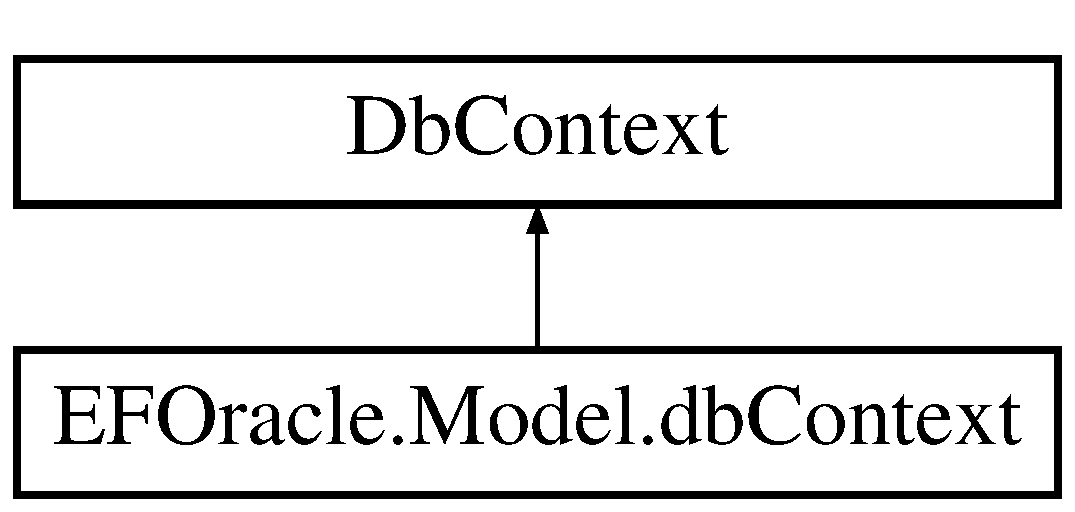
\includegraphics[height=2.000000cm]{class_e_f_oracle_1_1_model_1_1db_context}
\end{center}
\end{figure}
\subsection*{Public Member Functions}
\begin{DoxyCompactItemize}
\item 
\hyperlink{class_e_f_oracle_1_1_model_1_1db_context_a5583d9c5a470911b15527260b9974eb3}{db\+Context} ()
\end{DoxyCompactItemize}
\subsection*{Protected Member Functions}
\begin{DoxyCompactItemize}
\item 
override void \hyperlink{class_e_f_oracle_1_1_model_1_1db_context_ad16f374ba040f57b97167ea2decb2c85}{On\+Model\+Creating} (Db\+Model\+Builder model\+Builder)
\end{DoxyCompactItemize}
\subsection*{Properties}
\begin{DoxyCompactItemize}
\item 
virtual Db\+Set$<$ \hyperlink{class_e_f_oracle_1_1_model_1_1_d_i_s_c_i_p_l_i_n_e}{D\+I\+S\+C\+I\+P\+L\+I\+NE} $>$ \hyperlink{class_e_f_oracle_1_1_model_1_1db_context_a877177066e29d595f2dddfe607221014}{D\+I\+S\+C\+I\+P\+L\+I\+N\+Es}\hspace{0.3cm}{\ttfamily  \mbox{[}get, set\mbox{]}}
\item 
virtual Db\+Set$<$ \hyperlink{class_e_f_oracle_1_1_model_1_1_f_a_q}{F\+AQ} $>$ \hyperlink{class_e_f_oracle_1_1_model_1_1db_context_ae4d2109d575a8452d43c4a248b904ce9}{F\+A\+QS}\hspace{0.3cm}{\ttfamily  \mbox{[}get, set\mbox{]}}
\item 
virtual Db\+Set$<$ \hyperlink{class_e_f_oracle_1_1_model_1_1_g_r_o_u_p}{G\+R\+O\+UP} $>$ \hyperlink{class_e_f_oracle_1_1_model_1_1db_context_ac3341236bedc98c90e78823a2445ec77}{G\+R\+O\+U\+Ps}\hspace{0.3cm}{\ttfamily  \mbox{[}get, set\mbox{]}}
\item 
virtual Db\+Set$<$ \hyperlink{class_e_f_oracle_1_1_model_1_1_s_c_h_e_d_u_l_e}{S\+C\+H\+E\+D\+U\+LE} $>$ \hyperlink{class_e_f_oracle_1_1_model_1_1db_context_a8d28c1bcf1c322197797742fc19fb938}{S\+C\+H\+E\+D\+U\+L\+Es}\hspace{0.3cm}{\ttfamily  \mbox{[}get, set\mbox{]}}
\item 
virtual Db\+Set$<$ \hyperlink{class_e_f_oracle_1_1_model_1_1_s_t_u_d_e_n_t}{S\+T\+U\+D\+E\+NT} $>$ \hyperlink{class_e_f_oracle_1_1_model_1_1db_context_abc478c89d374a1536023b302d463999b}{S\+T\+U\+D\+E\+N\+Ts}\hspace{0.3cm}{\ttfamily  \mbox{[}get, set\mbox{]}}
\item 
virtual Db\+Set$<$ \hyperlink{class_e_f_oracle_1_1_model_1_1_s_t_u_d_e_n_t_w_o_r_k}{S\+T\+U\+D\+E\+N\+T\+W\+O\+RK} $>$ \hyperlink{class_e_f_oracle_1_1_model_1_1db_context_a20e83719134cb5ad1aacf084687d85f1}{S\+T\+U\+D\+E\+N\+T\+W\+O\+R\+Ks}\hspace{0.3cm}{\ttfamily  \mbox{[}get, set\mbox{]}}
\item 
virtual Db\+Set$<$ \hyperlink{class_e_f_oracle_1_1_model_1_1_t_a_s_k}{T\+A\+SK} $>$ \hyperlink{class_e_f_oracle_1_1_model_1_1db_context_aba64e3846cf54d7d09086057e8049442}{T\+A\+S\+Ks}\hspace{0.3cm}{\ttfamily  \mbox{[}get, set\mbox{]}}
\item 
virtual Db\+Set$<$ \hyperlink{class_e_f_oracle_1_1_model_1_1_t_a_s_k_t_y_p_e}{T\+A\+S\+K\+T\+Y\+PE} $>$ \hyperlink{class_e_f_oracle_1_1_model_1_1db_context_a943a716657ad3f7ccccbfa5a50e8cf0b}{T\+A\+S\+K\+T\+Y\+P\+ES}\hspace{0.3cm}{\ttfamily  \mbox{[}get, set\mbox{]}}
\item 
virtual Db\+Set$<$ \hyperlink{class_e_f_oracle_1_1_model_1_1_t_e_a_c_h_e_r}{T\+E\+A\+C\+H\+ER} $>$ \hyperlink{class_e_f_oracle_1_1_model_1_1db_context_ae314b6a52d4ba6dab7d47687f70ff1ae}{T\+E\+A\+C\+H\+E\+Rs}\hspace{0.3cm}{\ttfamily  \mbox{[}get, set\mbox{]}}
\item 
virtual Db\+Set$<$ \hyperlink{class_e_f_oracle_1_1_model_1_1_u_s_e_r}{U\+S\+ER} $>$ \hyperlink{class_e_f_oracle_1_1_model_1_1db_context_aa300c467cc435086d3610121fc2a6545}{U\+S\+E\+Rs}\hspace{0.3cm}{\ttfamily  \mbox{[}get, set\mbox{]}}
\item 
virtual Db\+Set$<$ \hyperlink{class_e_f_oracle_1_1_model_1_1_u_s_e_r___s_e_s_s_i_o_n}{U\+S\+E\+R\+\_\+\+S\+E\+S\+S\+I\+ON} $>$ \hyperlink{class_e_f_oracle_1_1_model_1_1db_context_a8b948de9dbd472af5e756d7f8aecd18f}{U\+S\+E\+R\+\_\+\+S\+E\+S\+S\+I\+ON}\hspace{0.3cm}{\ttfamily  \mbox{[}get, set\mbox{]}}
\end{DoxyCompactItemize}


\subsection{Constructor \& Destructor Documentation}
\mbox{\Hypertarget{class_e_f_oracle_1_1_model_1_1db_context_a5583d9c5a470911b15527260b9974eb3}\label{class_e_f_oracle_1_1_model_1_1db_context_a5583d9c5a470911b15527260b9974eb3}} 
\index{E\+F\+Oracle\+::\+Model\+::db\+Context@{E\+F\+Oracle\+::\+Model\+::db\+Context}!db\+Context@{db\+Context}}
\index{db\+Context@{db\+Context}!E\+F\+Oracle\+::\+Model\+::db\+Context@{E\+F\+Oracle\+::\+Model\+::db\+Context}}
\subsubsection{\texorpdfstring{db\+Context()}{dbContext()}}
{\footnotesize\ttfamily E\+F\+Oracle.\+Model.\+db\+Context.\+db\+Context (\begin{DoxyParamCaption}{ }\end{DoxyParamCaption})}



\subsection{Member Function Documentation}
\mbox{\Hypertarget{class_e_f_oracle_1_1_model_1_1db_context_ad16f374ba040f57b97167ea2decb2c85}\label{class_e_f_oracle_1_1_model_1_1db_context_ad16f374ba040f57b97167ea2decb2c85}} 
\index{E\+F\+Oracle\+::\+Model\+::db\+Context@{E\+F\+Oracle\+::\+Model\+::db\+Context}!On\+Model\+Creating@{On\+Model\+Creating}}
\index{On\+Model\+Creating@{On\+Model\+Creating}!E\+F\+Oracle\+::\+Model\+::db\+Context@{E\+F\+Oracle\+::\+Model\+::db\+Context}}
\subsubsection{\texorpdfstring{On\+Model\+Creating()}{OnModelCreating()}}
{\footnotesize\ttfamily override void E\+F\+Oracle.\+Model.\+db\+Context.\+On\+Model\+Creating (\begin{DoxyParamCaption}\item[{Db\+Model\+Builder}]{model\+Builder }\end{DoxyParamCaption})\hspace{0.3cm}{\ttfamily [protected]}}



\subsection{Property Documentation}
\mbox{\Hypertarget{class_e_f_oracle_1_1_model_1_1db_context_a877177066e29d595f2dddfe607221014}\label{class_e_f_oracle_1_1_model_1_1db_context_a877177066e29d595f2dddfe607221014}} 
\index{E\+F\+Oracle\+::\+Model\+::db\+Context@{E\+F\+Oracle\+::\+Model\+::db\+Context}!D\+I\+S\+C\+I\+P\+L\+I\+N\+Es@{D\+I\+S\+C\+I\+P\+L\+I\+N\+Es}}
\index{D\+I\+S\+C\+I\+P\+L\+I\+N\+Es@{D\+I\+S\+C\+I\+P\+L\+I\+N\+Es}!E\+F\+Oracle\+::\+Model\+::db\+Context@{E\+F\+Oracle\+::\+Model\+::db\+Context}}
\subsubsection{\texorpdfstring{D\+I\+S\+C\+I\+P\+L\+I\+N\+Es}{DISCIPLINEs}}
{\footnotesize\ttfamily virtual Db\+Set$<$\hyperlink{class_e_f_oracle_1_1_model_1_1_d_i_s_c_i_p_l_i_n_e}{D\+I\+S\+C\+I\+P\+L\+I\+NE}$>$ E\+F\+Oracle.\+Model.\+db\+Context.\+D\+I\+S\+C\+I\+P\+L\+I\+N\+Es\hspace{0.3cm}{\ttfamily [get]}, {\ttfamily [set]}}

\mbox{\Hypertarget{class_e_f_oracle_1_1_model_1_1db_context_ae4d2109d575a8452d43c4a248b904ce9}\label{class_e_f_oracle_1_1_model_1_1db_context_ae4d2109d575a8452d43c4a248b904ce9}} 
\index{E\+F\+Oracle\+::\+Model\+::db\+Context@{E\+F\+Oracle\+::\+Model\+::db\+Context}!F\+A\+QS@{F\+A\+QS}}
\index{F\+A\+QS@{F\+A\+QS}!E\+F\+Oracle\+::\+Model\+::db\+Context@{E\+F\+Oracle\+::\+Model\+::db\+Context}}
\subsubsection{\texorpdfstring{F\+A\+QS}{FAQS}}
{\footnotesize\ttfamily virtual Db\+Set$<$\hyperlink{class_e_f_oracle_1_1_model_1_1_f_a_q}{F\+AQ}$>$ E\+F\+Oracle.\+Model.\+db\+Context.\+F\+A\+QS\hspace{0.3cm}{\ttfamily [get]}, {\ttfamily [set]}}

\mbox{\Hypertarget{class_e_f_oracle_1_1_model_1_1db_context_ac3341236bedc98c90e78823a2445ec77}\label{class_e_f_oracle_1_1_model_1_1db_context_ac3341236bedc98c90e78823a2445ec77}} 
\index{E\+F\+Oracle\+::\+Model\+::db\+Context@{E\+F\+Oracle\+::\+Model\+::db\+Context}!G\+R\+O\+U\+Ps@{G\+R\+O\+U\+Ps}}
\index{G\+R\+O\+U\+Ps@{G\+R\+O\+U\+Ps}!E\+F\+Oracle\+::\+Model\+::db\+Context@{E\+F\+Oracle\+::\+Model\+::db\+Context}}
\subsubsection{\texorpdfstring{G\+R\+O\+U\+Ps}{GROUPs}}
{\footnotesize\ttfamily virtual Db\+Set$<$\hyperlink{class_e_f_oracle_1_1_model_1_1_g_r_o_u_p}{G\+R\+O\+UP}$>$ E\+F\+Oracle.\+Model.\+db\+Context.\+G\+R\+O\+U\+Ps\hspace{0.3cm}{\ttfamily [get]}, {\ttfamily [set]}}

\mbox{\Hypertarget{class_e_f_oracle_1_1_model_1_1db_context_a8d28c1bcf1c322197797742fc19fb938}\label{class_e_f_oracle_1_1_model_1_1db_context_a8d28c1bcf1c322197797742fc19fb938}} 
\index{E\+F\+Oracle\+::\+Model\+::db\+Context@{E\+F\+Oracle\+::\+Model\+::db\+Context}!S\+C\+H\+E\+D\+U\+L\+Es@{S\+C\+H\+E\+D\+U\+L\+Es}}
\index{S\+C\+H\+E\+D\+U\+L\+Es@{S\+C\+H\+E\+D\+U\+L\+Es}!E\+F\+Oracle\+::\+Model\+::db\+Context@{E\+F\+Oracle\+::\+Model\+::db\+Context}}
\subsubsection{\texorpdfstring{S\+C\+H\+E\+D\+U\+L\+Es}{SCHEDULEs}}
{\footnotesize\ttfamily virtual Db\+Set$<$\hyperlink{class_e_f_oracle_1_1_model_1_1_s_c_h_e_d_u_l_e}{S\+C\+H\+E\+D\+U\+LE}$>$ E\+F\+Oracle.\+Model.\+db\+Context.\+S\+C\+H\+E\+D\+U\+L\+Es\hspace{0.3cm}{\ttfamily [get]}, {\ttfamily [set]}}

\mbox{\Hypertarget{class_e_f_oracle_1_1_model_1_1db_context_abc478c89d374a1536023b302d463999b}\label{class_e_f_oracle_1_1_model_1_1db_context_abc478c89d374a1536023b302d463999b}} 
\index{E\+F\+Oracle\+::\+Model\+::db\+Context@{E\+F\+Oracle\+::\+Model\+::db\+Context}!S\+T\+U\+D\+E\+N\+Ts@{S\+T\+U\+D\+E\+N\+Ts}}
\index{S\+T\+U\+D\+E\+N\+Ts@{S\+T\+U\+D\+E\+N\+Ts}!E\+F\+Oracle\+::\+Model\+::db\+Context@{E\+F\+Oracle\+::\+Model\+::db\+Context}}
\subsubsection{\texorpdfstring{S\+T\+U\+D\+E\+N\+Ts}{STUDENTs}}
{\footnotesize\ttfamily virtual Db\+Set$<$\hyperlink{class_e_f_oracle_1_1_model_1_1_s_t_u_d_e_n_t}{S\+T\+U\+D\+E\+NT}$>$ E\+F\+Oracle.\+Model.\+db\+Context.\+S\+T\+U\+D\+E\+N\+Ts\hspace{0.3cm}{\ttfamily [get]}, {\ttfamily [set]}}

\mbox{\Hypertarget{class_e_f_oracle_1_1_model_1_1db_context_a20e83719134cb5ad1aacf084687d85f1}\label{class_e_f_oracle_1_1_model_1_1db_context_a20e83719134cb5ad1aacf084687d85f1}} 
\index{E\+F\+Oracle\+::\+Model\+::db\+Context@{E\+F\+Oracle\+::\+Model\+::db\+Context}!S\+T\+U\+D\+E\+N\+T\+W\+O\+R\+Ks@{S\+T\+U\+D\+E\+N\+T\+W\+O\+R\+Ks}}
\index{S\+T\+U\+D\+E\+N\+T\+W\+O\+R\+Ks@{S\+T\+U\+D\+E\+N\+T\+W\+O\+R\+Ks}!E\+F\+Oracle\+::\+Model\+::db\+Context@{E\+F\+Oracle\+::\+Model\+::db\+Context}}
\subsubsection{\texorpdfstring{S\+T\+U\+D\+E\+N\+T\+W\+O\+R\+Ks}{STUDENTWORKs}}
{\footnotesize\ttfamily virtual Db\+Set$<$\hyperlink{class_e_f_oracle_1_1_model_1_1_s_t_u_d_e_n_t_w_o_r_k}{S\+T\+U\+D\+E\+N\+T\+W\+O\+RK}$>$ E\+F\+Oracle.\+Model.\+db\+Context.\+S\+T\+U\+D\+E\+N\+T\+W\+O\+R\+Ks\hspace{0.3cm}{\ttfamily [get]}, {\ttfamily [set]}}

\mbox{\Hypertarget{class_e_f_oracle_1_1_model_1_1db_context_aba64e3846cf54d7d09086057e8049442}\label{class_e_f_oracle_1_1_model_1_1db_context_aba64e3846cf54d7d09086057e8049442}} 
\index{E\+F\+Oracle\+::\+Model\+::db\+Context@{E\+F\+Oracle\+::\+Model\+::db\+Context}!T\+A\+S\+Ks@{T\+A\+S\+Ks}}
\index{T\+A\+S\+Ks@{T\+A\+S\+Ks}!E\+F\+Oracle\+::\+Model\+::db\+Context@{E\+F\+Oracle\+::\+Model\+::db\+Context}}
\subsubsection{\texorpdfstring{T\+A\+S\+Ks}{TASKs}}
{\footnotesize\ttfamily virtual Db\+Set$<$\hyperlink{class_e_f_oracle_1_1_model_1_1_t_a_s_k}{T\+A\+SK}$>$ E\+F\+Oracle.\+Model.\+db\+Context.\+T\+A\+S\+Ks\hspace{0.3cm}{\ttfamily [get]}, {\ttfamily [set]}}

\mbox{\Hypertarget{class_e_f_oracle_1_1_model_1_1db_context_a943a716657ad3f7ccccbfa5a50e8cf0b}\label{class_e_f_oracle_1_1_model_1_1db_context_a943a716657ad3f7ccccbfa5a50e8cf0b}} 
\index{E\+F\+Oracle\+::\+Model\+::db\+Context@{E\+F\+Oracle\+::\+Model\+::db\+Context}!T\+A\+S\+K\+T\+Y\+P\+ES@{T\+A\+S\+K\+T\+Y\+P\+ES}}
\index{T\+A\+S\+K\+T\+Y\+P\+ES@{T\+A\+S\+K\+T\+Y\+P\+ES}!E\+F\+Oracle\+::\+Model\+::db\+Context@{E\+F\+Oracle\+::\+Model\+::db\+Context}}
\subsubsection{\texorpdfstring{T\+A\+S\+K\+T\+Y\+P\+ES}{TASKTYPES}}
{\footnotesize\ttfamily virtual Db\+Set$<$\hyperlink{class_e_f_oracle_1_1_model_1_1_t_a_s_k_t_y_p_e}{T\+A\+S\+K\+T\+Y\+PE}$>$ E\+F\+Oracle.\+Model.\+db\+Context.\+T\+A\+S\+K\+T\+Y\+P\+ES\hspace{0.3cm}{\ttfamily [get]}, {\ttfamily [set]}}

\mbox{\Hypertarget{class_e_f_oracle_1_1_model_1_1db_context_ae314b6a52d4ba6dab7d47687f70ff1ae}\label{class_e_f_oracle_1_1_model_1_1db_context_ae314b6a52d4ba6dab7d47687f70ff1ae}} 
\index{E\+F\+Oracle\+::\+Model\+::db\+Context@{E\+F\+Oracle\+::\+Model\+::db\+Context}!T\+E\+A\+C\+H\+E\+Rs@{T\+E\+A\+C\+H\+E\+Rs}}
\index{T\+E\+A\+C\+H\+E\+Rs@{T\+E\+A\+C\+H\+E\+Rs}!E\+F\+Oracle\+::\+Model\+::db\+Context@{E\+F\+Oracle\+::\+Model\+::db\+Context}}
\subsubsection{\texorpdfstring{T\+E\+A\+C\+H\+E\+Rs}{TEACHERs}}
{\footnotesize\ttfamily virtual Db\+Set$<$\hyperlink{class_e_f_oracle_1_1_model_1_1_t_e_a_c_h_e_r}{T\+E\+A\+C\+H\+ER}$>$ E\+F\+Oracle.\+Model.\+db\+Context.\+T\+E\+A\+C\+H\+E\+Rs\hspace{0.3cm}{\ttfamily [get]}, {\ttfamily [set]}}

\mbox{\Hypertarget{class_e_f_oracle_1_1_model_1_1db_context_a8b948de9dbd472af5e756d7f8aecd18f}\label{class_e_f_oracle_1_1_model_1_1db_context_a8b948de9dbd472af5e756d7f8aecd18f}} 
\index{E\+F\+Oracle\+::\+Model\+::db\+Context@{E\+F\+Oracle\+::\+Model\+::db\+Context}!U\+S\+E\+R\+\_\+\+S\+E\+S\+S\+I\+ON@{U\+S\+E\+R\+\_\+\+S\+E\+S\+S\+I\+ON}}
\index{U\+S\+E\+R\+\_\+\+S\+E\+S\+S\+I\+ON@{U\+S\+E\+R\+\_\+\+S\+E\+S\+S\+I\+ON}!E\+F\+Oracle\+::\+Model\+::db\+Context@{E\+F\+Oracle\+::\+Model\+::db\+Context}}
\subsubsection{\texorpdfstring{U\+S\+E\+R\+\_\+\+S\+E\+S\+S\+I\+ON}{USER\_SESSION}}
{\footnotesize\ttfamily virtual Db\+Set$<$\hyperlink{class_e_f_oracle_1_1_model_1_1_u_s_e_r___s_e_s_s_i_o_n}{U\+S\+E\+R\+\_\+\+S\+E\+S\+S\+I\+ON}$>$ E\+F\+Oracle.\+Model.\+db\+Context.\+U\+S\+E\+R\+\_\+\+S\+E\+S\+S\+I\+ON\hspace{0.3cm}{\ttfamily [get]}, {\ttfamily [set]}}

\mbox{\Hypertarget{class_e_f_oracle_1_1_model_1_1db_context_aa300c467cc435086d3610121fc2a6545}\label{class_e_f_oracle_1_1_model_1_1db_context_aa300c467cc435086d3610121fc2a6545}} 
\index{E\+F\+Oracle\+::\+Model\+::db\+Context@{E\+F\+Oracle\+::\+Model\+::db\+Context}!U\+S\+E\+Rs@{U\+S\+E\+Rs}}
\index{U\+S\+E\+Rs@{U\+S\+E\+Rs}!E\+F\+Oracle\+::\+Model\+::db\+Context@{E\+F\+Oracle\+::\+Model\+::db\+Context}}
\subsubsection{\texorpdfstring{U\+S\+E\+Rs}{USERs}}
{\footnotesize\ttfamily virtual Db\+Set$<$\hyperlink{class_e_f_oracle_1_1_model_1_1_u_s_e_r}{U\+S\+ER}$>$ E\+F\+Oracle.\+Model.\+db\+Context.\+U\+S\+E\+Rs\hspace{0.3cm}{\ttfamily [get]}, {\ttfamily [set]}}



The documentation for this class was generated from the following file\+:\begin{DoxyCompactItemize}
\item 
D\+:/\+\_\+\+W\+O\+R\+K/\+\_\+\+S\+T\+E\+P/\+In\+Study\+Asp/\+E\+F\+Oracle/\+Model/\hyperlink{db_context_8cs}{db\+Context.\+cs}\end{DoxyCompactItemize}

\hypertarget{class_e_f_oracle_1_1_model_1_1_d_i_s_c_i_p_l_i_n_e}{}\section{E\+F\+Oracle.\+Model.\+D\+I\+S\+C\+I\+P\+L\+I\+NE Class Reference}
\label{class_e_f_oracle_1_1_model_1_1_d_i_s_c_i_p_l_i_n_e}\index{E\+F\+Oracle.\+Model.\+D\+I\+S\+C\+I\+P\+L\+I\+NE@{E\+F\+Oracle.\+Model.\+D\+I\+S\+C\+I\+P\+L\+I\+NE}}
\subsection*{Public Member Functions}
\begin{DoxyCompactItemize}
\item 
\hyperlink{class_e_f_oracle_1_1_model_1_1_d_i_s_c_i_p_l_i_n_e_a7f1ccbe060471815839f602478f1d57b}{D\+I\+S\+C\+I\+P\+L\+I\+NE} ()
\end{DoxyCompactItemize}
\subsection*{Properties}
\begin{DoxyCompactItemize}
\item 
decimal \hyperlink{class_e_f_oracle_1_1_model_1_1_d_i_s_c_i_p_l_i_n_e_a567e03fdacbb6759c4c992661afebe35}{D\+I\+S\+C\+I\+P\+L\+I\+N\+E\+\_\+\+C\+O\+DE}\hspace{0.3cm}{\ttfamily  \mbox{[}get, set\mbox{]}}
\item 
string \hyperlink{class_e_f_oracle_1_1_model_1_1_d_i_s_c_i_p_l_i_n_e_a835096386d3c0f75cf242b1db2b6853b}{D\+I\+S\+C\+I\+P\+L\+I\+N\+E\+\_\+\+N\+A\+ME}\hspace{0.3cm}{\ttfamily  \mbox{[}get, set\mbox{]}}
\item 
virtual I\+Collection$<$ \hyperlink{class_e_f_oracle_1_1_model_1_1_s_c_h_e_d_u_l_e}{S\+C\+H\+E\+D\+U\+LE} $>$ \hyperlink{class_e_f_oracle_1_1_model_1_1_d_i_s_c_i_p_l_i_n_e_a88721dfdf505cfc7542013244720d12e}{S\+C\+H\+E\+D\+U\+L\+Es}\hspace{0.3cm}{\ttfamily  \mbox{[}get, set\mbox{]}}
\item 
virtual I\+Collection$<$ \hyperlink{class_e_f_oracle_1_1_model_1_1_t_a_s_k}{T\+A\+SK} $>$ \hyperlink{class_e_f_oracle_1_1_model_1_1_d_i_s_c_i_p_l_i_n_e_a729b4773e3441b7f9eb4cc65f74353ba}{T\+A\+S\+Ks}\hspace{0.3cm}{\ttfamily  \mbox{[}get, set\mbox{]}}
\end{DoxyCompactItemize}


\subsection{Constructor \& Destructor Documentation}
\mbox{\Hypertarget{class_e_f_oracle_1_1_model_1_1_d_i_s_c_i_p_l_i_n_e_a7f1ccbe060471815839f602478f1d57b}\label{class_e_f_oracle_1_1_model_1_1_d_i_s_c_i_p_l_i_n_e_a7f1ccbe060471815839f602478f1d57b}} 
\index{E\+F\+Oracle\+::\+Model\+::\+D\+I\+S\+C\+I\+P\+L\+I\+NE@{E\+F\+Oracle\+::\+Model\+::\+D\+I\+S\+C\+I\+P\+L\+I\+NE}!D\+I\+S\+C\+I\+P\+L\+I\+NE@{D\+I\+S\+C\+I\+P\+L\+I\+NE}}
\index{D\+I\+S\+C\+I\+P\+L\+I\+NE@{D\+I\+S\+C\+I\+P\+L\+I\+NE}!E\+F\+Oracle\+::\+Model\+::\+D\+I\+S\+C\+I\+P\+L\+I\+NE@{E\+F\+Oracle\+::\+Model\+::\+D\+I\+S\+C\+I\+P\+L\+I\+NE}}
\subsubsection{\texorpdfstring{D\+I\+S\+C\+I\+P\+L\+I\+N\+E()}{DISCIPLINE()}}
{\footnotesize\ttfamily E\+F\+Oracle.\+Model.\+D\+I\+S\+C\+I\+P\+L\+I\+N\+E.\+D\+I\+S\+C\+I\+P\+L\+I\+NE (\begin{DoxyParamCaption}{ }\end{DoxyParamCaption})}



\subsection{Property Documentation}
\mbox{\Hypertarget{class_e_f_oracle_1_1_model_1_1_d_i_s_c_i_p_l_i_n_e_a567e03fdacbb6759c4c992661afebe35}\label{class_e_f_oracle_1_1_model_1_1_d_i_s_c_i_p_l_i_n_e_a567e03fdacbb6759c4c992661afebe35}} 
\index{E\+F\+Oracle\+::\+Model\+::\+D\+I\+S\+C\+I\+P\+L\+I\+NE@{E\+F\+Oracle\+::\+Model\+::\+D\+I\+S\+C\+I\+P\+L\+I\+NE}!D\+I\+S\+C\+I\+P\+L\+I\+N\+E\+\_\+\+C\+O\+DE@{D\+I\+S\+C\+I\+P\+L\+I\+N\+E\+\_\+\+C\+O\+DE}}
\index{D\+I\+S\+C\+I\+P\+L\+I\+N\+E\+\_\+\+C\+O\+DE@{D\+I\+S\+C\+I\+P\+L\+I\+N\+E\+\_\+\+C\+O\+DE}!E\+F\+Oracle\+::\+Model\+::\+D\+I\+S\+C\+I\+P\+L\+I\+NE@{E\+F\+Oracle\+::\+Model\+::\+D\+I\+S\+C\+I\+P\+L\+I\+NE}}
\subsubsection{\texorpdfstring{D\+I\+S\+C\+I\+P\+L\+I\+N\+E\+\_\+\+C\+O\+DE}{DISCIPLINE\_CODE}}
{\footnotesize\ttfamily decimal E\+F\+Oracle.\+Model.\+D\+I\+S\+C\+I\+P\+L\+I\+N\+E.\+D\+I\+S\+C\+I\+P\+L\+I\+N\+E\+\_\+\+C\+O\+DE\hspace{0.3cm}{\ttfamily [get]}, {\ttfamily [set]}}

\mbox{\Hypertarget{class_e_f_oracle_1_1_model_1_1_d_i_s_c_i_p_l_i_n_e_a835096386d3c0f75cf242b1db2b6853b}\label{class_e_f_oracle_1_1_model_1_1_d_i_s_c_i_p_l_i_n_e_a835096386d3c0f75cf242b1db2b6853b}} 
\index{E\+F\+Oracle\+::\+Model\+::\+D\+I\+S\+C\+I\+P\+L\+I\+NE@{E\+F\+Oracle\+::\+Model\+::\+D\+I\+S\+C\+I\+P\+L\+I\+NE}!D\+I\+S\+C\+I\+P\+L\+I\+N\+E\+\_\+\+N\+A\+ME@{D\+I\+S\+C\+I\+P\+L\+I\+N\+E\+\_\+\+N\+A\+ME}}
\index{D\+I\+S\+C\+I\+P\+L\+I\+N\+E\+\_\+\+N\+A\+ME@{D\+I\+S\+C\+I\+P\+L\+I\+N\+E\+\_\+\+N\+A\+ME}!E\+F\+Oracle\+::\+Model\+::\+D\+I\+S\+C\+I\+P\+L\+I\+NE@{E\+F\+Oracle\+::\+Model\+::\+D\+I\+S\+C\+I\+P\+L\+I\+NE}}
\subsubsection{\texorpdfstring{D\+I\+S\+C\+I\+P\+L\+I\+N\+E\+\_\+\+N\+A\+ME}{DISCIPLINE\_NAME}}
{\footnotesize\ttfamily string E\+F\+Oracle.\+Model.\+D\+I\+S\+C\+I\+P\+L\+I\+N\+E.\+D\+I\+S\+C\+I\+P\+L\+I\+N\+E\+\_\+\+N\+A\+ME\hspace{0.3cm}{\ttfamily [get]}, {\ttfamily [set]}}

\mbox{\Hypertarget{class_e_f_oracle_1_1_model_1_1_d_i_s_c_i_p_l_i_n_e_a88721dfdf505cfc7542013244720d12e}\label{class_e_f_oracle_1_1_model_1_1_d_i_s_c_i_p_l_i_n_e_a88721dfdf505cfc7542013244720d12e}} 
\index{E\+F\+Oracle\+::\+Model\+::\+D\+I\+S\+C\+I\+P\+L\+I\+NE@{E\+F\+Oracle\+::\+Model\+::\+D\+I\+S\+C\+I\+P\+L\+I\+NE}!S\+C\+H\+E\+D\+U\+L\+Es@{S\+C\+H\+E\+D\+U\+L\+Es}}
\index{S\+C\+H\+E\+D\+U\+L\+Es@{S\+C\+H\+E\+D\+U\+L\+Es}!E\+F\+Oracle\+::\+Model\+::\+D\+I\+S\+C\+I\+P\+L\+I\+NE@{E\+F\+Oracle\+::\+Model\+::\+D\+I\+S\+C\+I\+P\+L\+I\+NE}}
\subsubsection{\texorpdfstring{S\+C\+H\+E\+D\+U\+L\+Es}{SCHEDULEs}}
{\footnotesize\ttfamily virtual I\+Collection$<$\hyperlink{class_e_f_oracle_1_1_model_1_1_s_c_h_e_d_u_l_e}{S\+C\+H\+E\+D\+U\+LE}$>$ E\+F\+Oracle.\+Model.\+D\+I\+S\+C\+I\+P\+L\+I\+N\+E.\+S\+C\+H\+E\+D\+U\+L\+Es\hspace{0.3cm}{\ttfamily [get]}, {\ttfamily [set]}}

\mbox{\Hypertarget{class_e_f_oracle_1_1_model_1_1_d_i_s_c_i_p_l_i_n_e_a729b4773e3441b7f9eb4cc65f74353ba}\label{class_e_f_oracle_1_1_model_1_1_d_i_s_c_i_p_l_i_n_e_a729b4773e3441b7f9eb4cc65f74353ba}} 
\index{E\+F\+Oracle\+::\+Model\+::\+D\+I\+S\+C\+I\+P\+L\+I\+NE@{E\+F\+Oracle\+::\+Model\+::\+D\+I\+S\+C\+I\+P\+L\+I\+NE}!T\+A\+S\+Ks@{T\+A\+S\+Ks}}
\index{T\+A\+S\+Ks@{T\+A\+S\+Ks}!E\+F\+Oracle\+::\+Model\+::\+D\+I\+S\+C\+I\+P\+L\+I\+NE@{E\+F\+Oracle\+::\+Model\+::\+D\+I\+S\+C\+I\+P\+L\+I\+NE}}
\subsubsection{\texorpdfstring{T\+A\+S\+Ks}{TASKs}}
{\footnotesize\ttfamily virtual I\+Collection$<$\hyperlink{class_e_f_oracle_1_1_model_1_1_t_a_s_k}{T\+A\+SK}$>$ E\+F\+Oracle.\+Model.\+D\+I\+S\+C\+I\+P\+L\+I\+N\+E.\+T\+A\+S\+Ks\hspace{0.3cm}{\ttfamily [get]}, {\ttfamily [set]}}



The documentation for this class was generated from the following file\+:\begin{DoxyCompactItemize}
\item 
D\+:/\+\_\+\+W\+O\+R\+K/\+\_\+\+S\+T\+E\+P/\+In\+Study\+Asp/\+E\+F\+Oracle/\+Model/\hyperlink{_d_i_s_c_i_p_l_i_n_e_8cs}{D\+I\+S\+C\+I\+P\+L\+I\+N\+E.\+cs}\end{DoxyCompactItemize}

\hypertarget{class_repo_1_1_discipline_repository}{}\section{Repo.\+Discipline\+Repository Class Reference}
\label{class_repo_1_1_discipline_repository}\index{Repo.\+Discipline\+Repository@{Repo.\+Discipline\+Repository}}
Inheritance diagram for Repo.\+Discipline\+Repository\+:\begin{figure}[H]
\begin{center}
\leavevmode
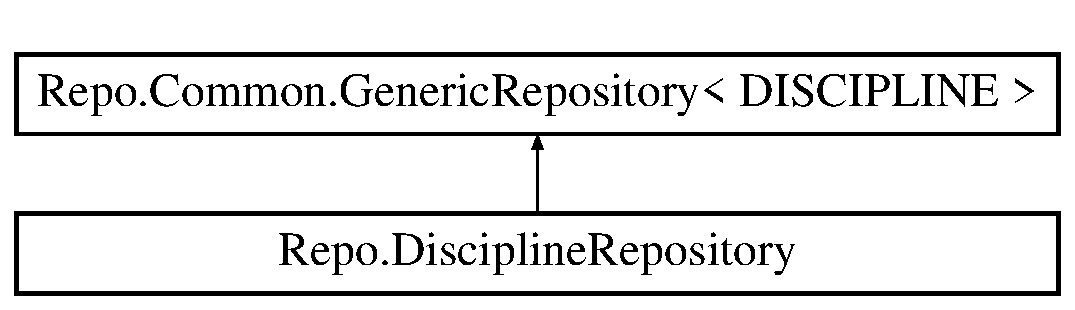
\includegraphics[height=2.000000cm]{class_repo_1_1_discipline_repository}
\end{center}
\end{figure}
\subsection*{Public Member Functions}
\begin{DoxyCompactItemize}
\item 
\hyperlink{class_repo_1_1_discipline_repository_afa2affb6e48433534bbba785fb6b29b8}{Discipline\+Repository} (\hyperlink{class_e_f_oracle_1_1_model_1_1db_context}{db\+Context} context)
\end{DoxyCompactItemize}
\subsection*{Additional Inherited Members}


\subsection{Constructor \& Destructor Documentation}
\mbox{\Hypertarget{class_repo_1_1_discipline_repository_afa2affb6e48433534bbba785fb6b29b8}\label{class_repo_1_1_discipline_repository_afa2affb6e48433534bbba785fb6b29b8}} 
\index{Repo\+::\+Discipline\+Repository@{Repo\+::\+Discipline\+Repository}!Discipline\+Repository@{Discipline\+Repository}}
\index{Discipline\+Repository@{Discipline\+Repository}!Repo\+::\+Discipline\+Repository@{Repo\+::\+Discipline\+Repository}}
\subsubsection{\texorpdfstring{Discipline\+Repository()}{DisciplineRepository()}}
{\footnotesize\ttfamily Repo.\+Discipline\+Repository.\+Discipline\+Repository (\begin{DoxyParamCaption}\item[{\hyperlink{class_e_f_oracle_1_1_model_1_1db_context}{db\+Context}}]{context }\end{DoxyParamCaption})}



The documentation for this class was generated from the following file\+:\begin{DoxyCompactItemize}
\item 
D\+:/\+\_\+\+W\+O\+R\+K/\+\_\+\+S\+T\+E\+P/\+In\+Study\+Asp/\+Repo/\hyperlink{_discipline_repository_8cs}{Discipline\+Repository.\+cs}\end{DoxyCompactItemize}

\hypertarget{class_e_f_oracle_1_1_model_1_1_f_a_q}{}\section{E\+F\+Oracle.\+Model.\+F\+AQ Class Reference}
\label{class_e_f_oracle_1_1_model_1_1_f_a_q}\index{E\+F\+Oracle.\+Model.\+F\+AQ@{E\+F\+Oracle.\+Model.\+F\+AQ}}
\subsection*{Properties}
\begin{DoxyCompactItemize}
\item 
decimal \hyperlink{class_e_f_oracle_1_1_model_1_1_f_a_q_a0bcf83da72276f02028f8acfaed304a7}{S\+T\+U\+D\+E\+N\+T\+\_\+\+ID}\hspace{0.3cm}{\ttfamily  \mbox{[}get, set\mbox{]}}
\item 
decimal \hyperlink{class_e_f_oracle_1_1_model_1_1_f_a_q_ac119f0ed74ccfd75000b6c3457b3b010}{T\+A\+S\+K\+\_\+\+ID}\hspace{0.3cm}{\ttfamily  \mbox{[}get, set\mbox{]}}
\item 
Date\+Time \hyperlink{class_e_f_oracle_1_1_model_1_1_f_a_q_acb0842a60775afbd015e10a437f3e236}{F\+A\+Q\+S\+\_\+\+Q\+U\+E\+S\+T\+I\+O\+N\+\_\+\+T\+I\+ME}\hspace{0.3cm}{\ttfamily  \mbox{[}get, set\mbox{]}}
\item 
string \hyperlink{class_e_f_oracle_1_1_model_1_1_f_a_q_a65d95d519d8fc525edc85497a0749e42}{F\+A\+Q\+S\+\_\+\+Q\+U\+E\+S\+T\+I\+ON}\hspace{0.3cm}{\ttfamily  \mbox{[}get, set\mbox{]}}
\item 
decimal \hyperlink{class_e_f_oracle_1_1_model_1_1_f_a_q_a3eac2b0318527689b32ef3d14ada8c8e}{T\+E\+A\+C\+H\+E\+R\+\_\+\+ID}\hspace{0.3cm}{\ttfamily  \mbox{[}get, set\mbox{]}}
\item 
Date\+Time \hyperlink{class_e_f_oracle_1_1_model_1_1_f_a_q_a3a5dbd4785eab45b01e3cae25ee9de44}{F\+A\+Q\+S\+\_\+\+A\+N\+S\+W\+E\+R\+\_\+\+T\+I\+ME}\hspace{0.3cm}{\ttfamily  \mbox{[}get, set\mbox{]}}
\item 
string \hyperlink{class_e_f_oracle_1_1_model_1_1_f_a_q_a1d272a26042ec0b0d0b75fa2d4a1efb6}{F\+A\+Q\+S\+\_\+\+A\+N\+S\+W\+ER}\hspace{0.3cm}{\ttfamily  \mbox{[}get, set\mbox{]}}
\item 
virtual \hyperlink{class_e_f_oracle_1_1_model_1_1_s_t_u_d_e_n_t}{S\+T\+U\+D\+E\+NT} \hyperlink{class_e_f_oracle_1_1_model_1_1_f_a_q_aedf902539902e76ef64411fd4dac62b2}{S\+T\+U\+D\+E\+NT}\hspace{0.3cm}{\ttfamily  \mbox{[}get, set\mbox{]}}
\item 
virtual \hyperlink{class_e_f_oracle_1_1_model_1_1_t_a_s_k}{T\+A\+SK} \hyperlink{class_e_f_oracle_1_1_model_1_1_f_a_q_a37d257d9c330a1fab7dfa6090e79628f}{T\+A\+SK}\hspace{0.3cm}{\ttfamily  \mbox{[}get, set\mbox{]}}
\item 
virtual \hyperlink{class_e_f_oracle_1_1_model_1_1_t_e_a_c_h_e_r}{T\+E\+A\+C\+H\+ER} \hyperlink{class_e_f_oracle_1_1_model_1_1_f_a_q_ab91ab3cc5c2ebf1a7053f2740ab47b3d}{T\+E\+A\+C\+H\+ER}\hspace{0.3cm}{\ttfamily  \mbox{[}get, set\mbox{]}}
\end{DoxyCompactItemize}


\subsection{Property Documentation}
\mbox{\Hypertarget{class_e_f_oracle_1_1_model_1_1_f_a_q_a1d272a26042ec0b0d0b75fa2d4a1efb6}\label{class_e_f_oracle_1_1_model_1_1_f_a_q_a1d272a26042ec0b0d0b75fa2d4a1efb6}} 
\index{E\+F\+Oracle\+::\+Model\+::\+F\+AQ@{E\+F\+Oracle\+::\+Model\+::\+F\+AQ}!F\+A\+Q\+S\+\_\+\+A\+N\+S\+W\+ER@{F\+A\+Q\+S\+\_\+\+A\+N\+S\+W\+ER}}
\index{F\+A\+Q\+S\+\_\+\+A\+N\+S\+W\+ER@{F\+A\+Q\+S\+\_\+\+A\+N\+S\+W\+ER}!E\+F\+Oracle\+::\+Model\+::\+F\+AQ@{E\+F\+Oracle\+::\+Model\+::\+F\+AQ}}
\subsubsection{\texorpdfstring{F\+A\+Q\+S\+\_\+\+A\+N\+S\+W\+ER}{FAQS\_ANSWER}}
{\footnotesize\ttfamily string E\+F\+Oracle.\+Model.\+F\+A\+Q.\+F\+A\+Q\+S\+\_\+\+A\+N\+S\+W\+ER\hspace{0.3cm}{\ttfamily [get]}, {\ttfamily [set]}}

\mbox{\Hypertarget{class_e_f_oracle_1_1_model_1_1_f_a_q_a3a5dbd4785eab45b01e3cae25ee9de44}\label{class_e_f_oracle_1_1_model_1_1_f_a_q_a3a5dbd4785eab45b01e3cae25ee9de44}} 
\index{E\+F\+Oracle\+::\+Model\+::\+F\+AQ@{E\+F\+Oracle\+::\+Model\+::\+F\+AQ}!F\+A\+Q\+S\+\_\+\+A\+N\+S\+W\+E\+R\+\_\+\+T\+I\+ME@{F\+A\+Q\+S\+\_\+\+A\+N\+S\+W\+E\+R\+\_\+\+T\+I\+ME}}
\index{F\+A\+Q\+S\+\_\+\+A\+N\+S\+W\+E\+R\+\_\+\+T\+I\+ME@{F\+A\+Q\+S\+\_\+\+A\+N\+S\+W\+E\+R\+\_\+\+T\+I\+ME}!E\+F\+Oracle\+::\+Model\+::\+F\+AQ@{E\+F\+Oracle\+::\+Model\+::\+F\+AQ}}
\subsubsection{\texorpdfstring{F\+A\+Q\+S\+\_\+\+A\+N\+S\+W\+E\+R\+\_\+\+T\+I\+ME}{FAQS\_ANSWER\_TIME}}
{\footnotesize\ttfamily Date\+Time E\+F\+Oracle.\+Model.\+F\+A\+Q.\+F\+A\+Q\+S\+\_\+\+A\+N\+S\+W\+E\+R\+\_\+\+T\+I\+ME\hspace{0.3cm}{\ttfamily [get]}, {\ttfamily [set]}}

\mbox{\Hypertarget{class_e_f_oracle_1_1_model_1_1_f_a_q_a65d95d519d8fc525edc85497a0749e42}\label{class_e_f_oracle_1_1_model_1_1_f_a_q_a65d95d519d8fc525edc85497a0749e42}} 
\index{E\+F\+Oracle\+::\+Model\+::\+F\+AQ@{E\+F\+Oracle\+::\+Model\+::\+F\+AQ}!F\+A\+Q\+S\+\_\+\+Q\+U\+E\+S\+T\+I\+ON@{F\+A\+Q\+S\+\_\+\+Q\+U\+E\+S\+T\+I\+ON}}
\index{F\+A\+Q\+S\+\_\+\+Q\+U\+E\+S\+T\+I\+ON@{F\+A\+Q\+S\+\_\+\+Q\+U\+E\+S\+T\+I\+ON}!E\+F\+Oracle\+::\+Model\+::\+F\+AQ@{E\+F\+Oracle\+::\+Model\+::\+F\+AQ}}
\subsubsection{\texorpdfstring{F\+A\+Q\+S\+\_\+\+Q\+U\+E\+S\+T\+I\+ON}{FAQS\_QUESTION}}
{\footnotesize\ttfamily string E\+F\+Oracle.\+Model.\+F\+A\+Q.\+F\+A\+Q\+S\+\_\+\+Q\+U\+E\+S\+T\+I\+ON\hspace{0.3cm}{\ttfamily [get]}, {\ttfamily [set]}}

\mbox{\Hypertarget{class_e_f_oracle_1_1_model_1_1_f_a_q_acb0842a60775afbd015e10a437f3e236}\label{class_e_f_oracle_1_1_model_1_1_f_a_q_acb0842a60775afbd015e10a437f3e236}} 
\index{E\+F\+Oracle\+::\+Model\+::\+F\+AQ@{E\+F\+Oracle\+::\+Model\+::\+F\+AQ}!F\+A\+Q\+S\+\_\+\+Q\+U\+E\+S\+T\+I\+O\+N\+\_\+\+T\+I\+ME@{F\+A\+Q\+S\+\_\+\+Q\+U\+E\+S\+T\+I\+O\+N\+\_\+\+T\+I\+ME}}
\index{F\+A\+Q\+S\+\_\+\+Q\+U\+E\+S\+T\+I\+O\+N\+\_\+\+T\+I\+ME@{F\+A\+Q\+S\+\_\+\+Q\+U\+E\+S\+T\+I\+O\+N\+\_\+\+T\+I\+ME}!E\+F\+Oracle\+::\+Model\+::\+F\+AQ@{E\+F\+Oracle\+::\+Model\+::\+F\+AQ}}
\subsubsection{\texorpdfstring{F\+A\+Q\+S\+\_\+\+Q\+U\+E\+S\+T\+I\+O\+N\+\_\+\+T\+I\+ME}{FAQS\_QUESTION\_TIME}}
{\footnotesize\ttfamily Date\+Time E\+F\+Oracle.\+Model.\+F\+A\+Q.\+F\+A\+Q\+S\+\_\+\+Q\+U\+E\+S\+T\+I\+O\+N\+\_\+\+T\+I\+ME\hspace{0.3cm}{\ttfamily [get]}, {\ttfamily [set]}}

\mbox{\Hypertarget{class_e_f_oracle_1_1_model_1_1_f_a_q_aedf902539902e76ef64411fd4dac62b2}\label{class_e_f_oracle_1_1_model_1_1_f_a_q_aedf902539902e76ef64411fd4dac62b2}} 
\index{E\+F\+Oracle\+::\+Model\+::\+F\+AQ@{E\+F\+Oracle\+::\+Model\+::\+F\+AQ}!S\+T\+U\+D\+E\+NT@{S\+T\+U\+D\+E\+NT}}
\index{S\+T\+U\+D\+E\+NT@{S\+T\+U\+D\+E\+NT}!E\+F\+Oracle\+::\+Model\+::\+F\+AQ@{E\+F\+Oracle\+::\+Model\+::\+F\+AQ}}
\subsubsection{\texorpdfstring{S\+T\+U\+D\+E\+NT}{STUDENT}}
{\footnotesize\ttfamily virtual \hyperlink{class_e_f_oracle_1_1_model_1_1_s_t_u_d_e_n_t}{S\+T\+U\+D\+E\+NT} E\+F\+Oracle.\+Model.\+F\+A\+Q.\+S\+T\+U\+D\+E\+NT\hspace{0.3cm}{\ttfamily [get]}, {\ttfamily [set]}}

\mbox{\Hypertarget{class_e_f_oracle_1_1_model_1_1_f_a_q_a0bcf83da72276f02028f8acfaed304a7}\label{class_e_f_oracle_1_1_model_1_1_f_a_q_a0bcf83da72276f02028f8acfaed304a7}} 
\index{E\+F\+Oracle\+::\+Model\+::\+F\+AQ@{E\+F\+Oracle\+::\+Model\+::\+F\+AQ}!S\+T\+U\+D\+E\+N\+T\+\_\+\+ID@{S\+T\+U\+D\+E\+N\+T\+\_\+\+ID}}
\index{S\+T\+U\+D\+E\+N\+T\+\_\+\+ID@{S\+T\+U\+D\+E\+N\+T\+\_\+\+ID}!E\+F\+Oracle\+::\+Model\+::\+F\+AQ@{E\+F\+Oracle\+::\+Model\+::\+F\+AQ}}
\subsubsection{\texorpdfstring{S\+T\+U\+D\+E\+N\+T\+\_\+\+ID}{STUDENT\_ID}}
{\footnotesize\ttfamily decimal E\+F\+Oracle.\+Model.\+F\+A\+Q.\+S\+T\+U\+D\+E\+N\+T\+\_\+\+ID\hspace{0.3cm}{\ttfamily [get]}, {\ttfamily [set]}}

\mbox{\Hypertarget{class_e_f_oracle_1_1_model_1_1_f_a_q_a37d257d9c330a1fab7dfa6090e79628f}\label{class_e_f_oracle_1_1_model_1_1_f_a_q_a37d257d9c330a1fab7dfa6090e79628f}} 
\index{E\+F\+Oracle\+::\+Model\+::\+F\+AQ@{E\+F\+Oracle\+::\+Model\+::\+F\+AQ}!T\+A\+SK@{T\+A\+SK}}
\index{T\+A\+SK@{T\+A\+SK}!E\+F\+Oracle\+::\+Model\+::\+F\+AQ@{E\+F\+Oracle\+::\+Model\+::\+F\+AQ}}
\subsubsection{\texorpdfstring{T\+A\+SK}{TASK}}
{\footnotesize\ttfamily virtual \hyperlink{class_e_f_oracle_1_1_model_1_1_t_a_s_k}{T\+A\+SK} E\+F\+Oracle.\+Model.\+F\+A\+Q.\+T\+A\+SK\hspace{0.3cm}{\ttfamily [get]}, {\ttfamily [set]}}

\mbox{\Hypertarget{class_e_f_oracle_1_1_model_1_1_f_a_q_ac119f0ed74ccfd75000b6c3457b3b010}\label{class_e_f_oracle_1_1_model_1_1_f_a_q_ac119f0ed74ccfd75000b6c3457b3b010}} 
\index{E\+F\+Oracle\+::\+Model\+::\+F\+AQ@{E\+F\+Oracle\+::\+Model\+::\+F\+AQ}!T\+A\+S\+K\+\_\+\+ID@{T\+A\+S\+K\+\_\+\+ID}}
\index{T\+A\+S\+K\+\_\+\+ID@{T\+A\+S\+K\+\_\+\+ID}!E\+F\+Oracle\+::\+Model\+::\+F\+AQ@{E\+F\+Oracle\+::\+Model\+::\+F\+AQ}}
\subsubsection{\texorpdfstring{T\+A\+S\+K\+\_\+\+ID}{TASK\_ID}}
{\footnotesize\ttfamily decimal E\+F\+Oracle.\+Model.\+F\+A\+Q.\+T\+A\+S\+K\+\_\+\+ID\hspace{0.3cm}{\ttfamily [get]}, {\ttfamily [set]}}

\mbox{\Hypertarget{class_e_f_oracle_1_1_model_1_1_f_a_q_ab91ab3cc5c2ebf1a7053f2740ab47b3d}\label{class_e_f_oracle_1_1_model_1_1_f_a_q_ab91ab3cc5c2ebf1a7053f2740ab47b3d}} 
\index{E\+F\+Oracle\+::\+Model\+::\+F\+AQ@{E\+F\+Oracle\+::\+Model\+::\+F\+AQ}!T\+E\+A\+C\+H\+ER@{T\+E\+A\+C\+H\+ER}}
\index{T\+E\+A\+C\+H\+ER@{T\+E\+A\+C\+H\+ER}!E\+F\+Oracle\+::\+Model\+::\+F\+AQ@{E\+F\+Oracle\+::\+Model\+::\+F\+AQ}}
\subsubsection{\texorpdfstring{T\+E\+A\+C\+H\+ER}{TEACHER}}
{\footnotesize\ttfamily virtual \hyperlink{class_e_f_oracle_1_1_model_1_1_t_e_a_c_h_e_r}{T\+E\+A\+C\+H\+ER} E\+F\+Oracle.\+Model.\+F\+A\+Q.\+T\+E\+A\+C\+H\+ER\hspace{0.3cm}{\ttfamily [get]}, {\ttfamily [set]}}

\mbox{\Hypertarget{class_e_f_oracle_1_1_model_1_1_f_a_q_a3eac2b0318527689b32ef3d14ada8c8e}\label{class_e_f_oracle_1_1_model_1_1_f_a_q_a3eac2b0318527689b32ef3d14ada8c8e}} 
\index{E\+F\+Oracle\+::\+Model\+::\+F\+AQ@{E\+F\+Oracle\+::\+Model\+::\+F\+AQ}!T\+E\+A\+C\+H\+E\+R\+\_\+\+ID@{T\+E\+A\+C\+H\+E\+R\+\_\+\+ID}}
\index{T\+E\+A\+C\+H\+E\+R\+\_\+\+ID@{T\+E\+A\+C\+H\+E\+R\+\_\+\+ID}!E\+F\+Oracle\+::\+Model\+::\+F\+AQ@{E\+F\+Oracle\+::\+Model\+::\+F\+AQ}}
\subsubsection{\texorpdfstring{T\+E\+A\+C\+H\+E\+R\+\_\+\+ID}{TEACHER\_ID}}
{\footnotesize\ttfamily decimal E\+F\+Oracle.\+Model.\+F\+A\+Q.\+T\+E\+A\+C\+H\+E\+R\+\_\+\+ID\hspace{0.3cm}{\ttfamily [get]}, {\ttfamily [set]}}



The documentation for this class was generated from the following file\+:\begin{DoxyCompactItemize}
\item 
D\+:/\+\_\+\+W\+O\+R\+K/\+\_\+\+S\+T\+E\+P/\+In\+Study\+Asp/\+E\+F\+Oracle/\+Model/\hyperlink{_f_a_q_8cs}{F\+A\+Q.\+cs}\end{DoxyCompactItemize}

\hypertarget{class_repo_1_1_common_1_1_generic_repository}{}\section{Repo.\+Common.\+Generic\+Repository$<$ T $>$ Class Template Reference}
\label{class_repo_1_1_common_1_1_generic_repository}\index{Repo.\+Common.\+Generic\+Repository$<$ T $>$@{Repo.\+Common.\+Generic\+Repository$<$ T $>$}}
Inheritance diagram for Repo.\+Common.\+Generic\+Repository$<$ T $>$\+:\begin{figure}[H]
\begin{center}
\leavevmode
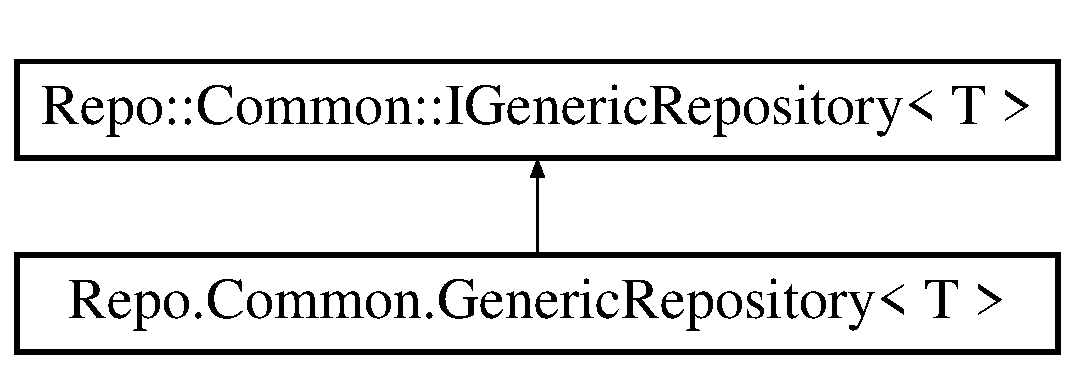
\includegraphics[height=2.000000cm]{class_repo_1_1_common_1_1_generic_repository}
\end{center}
\end{figure}
\subsection*{Public Member Functions}
\begin{DoxyCompactItemize}
\item 
\hyperlink{class_repo_1_1_common_1_1_generic_repository_a6ad38e9dd280fddbbf25be2e8e1bd88a}{Generic\+Repository} (Db\+Context context)
\item 
virtual I\+Enumerable$<$ T $>$ \hyperlink{class_repo_1_1_common_1_1_generic_repository_a819ba9c87b3246d17672f348c2162c7f}{Get\+All} ()
\item 
I\+Enumerable$<$ T $>$ \hyperlink{class_repo_1_1_common_1_1_generic_repository_a6126ca7ac03f92d7b51eefb2d023a151}{Find\+By} (System.\+Linq.\+Expressions.\+Expression$<$ Func$<$ T, bool $>$$>$ predicate)
\item 
virtual T \hyperlink{class_repo_1_1_common_1_1_generic_repository_ac3f609e57fb59eee8b0d8aaf2d1dd220}{Get} (int id)
\item 
virtual void \hyperlink{class_repo_1_1_common_1_1_generic_repository_a2370df477136ac65eacb282af1d00a9c}{Add\+Or\+Update} (T entity)
\item 
virtual void \hyperlink{class_repo_1_1_common_1_1_generic_repository_a9714e5c61c4f3541137bb83bebe054bb}{Delete} (T entity)
\item 
virtual void \hyperlink{class_repo_1_1_common_1_1_generic_repository_ab66ace5b2cc69867ce37dc996fc6c6e8}{Save} ()
\end{DoxyCompactItemize}
\subsection*{Protected Attributes}
\begin{DoxyCompactItemize}
\item 
Db\+Context \hyperlink{class_repo_1_1_common_1_1_generic_repository_a24c97c27d80ffec6a2c058a183b5941e}{\+\_\+entities}
\item 
readonly I\+Db\+Set$<$ T $>$ \hyperlink{class_repo_1_1_common_1_1_generic_repository_a921e230c30c21f3adeb8f7ffd6345149}{\+\_\+dbset}
\end{DoxyCompactItemize}


\subsection{Constructor \& Destructor Documentation}
\mbox{\Hypertarget{class_repo_1_1_common_1_1_generic_repository_a6ad38e9dd280fddbbf25be2e8e1bd88a}\label{class_repo_1_1_common_1_1_generic_repository_a6ad38e9dd280fddbbf25be2e8e1bd88a}} 
\index{Repo\+::\+Common\+::\+Generic\+Repository@{Repo\+::\+Common\+::\+Generic\+Repository}!Generic\+Repository@{Generic\+Repository}}
\index{Generic\+Repository@{Generic\+Repository}!Repo\+::\+Common\+::\+Generic\+Repository@{Repo\+::\+Common\+::\+Generic\+Repository}}
\subsubsection{\texorpdfstring{Generic\+Repository()}{GenericRepository()}}
{\footnotesize\ttfamily \hyperlink{class_repo_1_1_common_1_1_generic_repository}{Repo.\+Common.\+Generic\+Repository}$<$ T $>$.\hyperlink{class_repo_1_1_common_1_1_generic_repository}{Generic\+Repository} (\begin{DoxyParamCaption}\item[{Db\+Context}]{context }\end{DoxyParamCaption})}



\subsection{Member Function Documentation}
\mbox{\Hypertarget{class_repo_1_1_common_1_1_generic_repository_a2370df477136ac65eacb282af1d00a9c}\label{class_repo_1_1_common_1_1_generic_repository_a2370df477136ac65eacb282af1d00a9c}} 
\index{Repo\+::\+Common\+::\+Generic\+Repository@{Repo\+::\+Common\+::\+Generic\+Repository}!Add\+Or\+Update@{Add\+Or\+Update}}
\index{Add\+Or\+Update@{Add\+Or\+Update}!Repo\+::\+Common\+::\+Generic\+Repository@{Repo\+::\+Common\+::\+Generic\+Repository}}
\subsubsection{\texorpdfstring{Add\+Or\+Update()}{AddOrUpdate()}}
{\footnotesize\ttfamily virtual void \hyperlink{class_repo_1_1_common_1_1_generic_repository}{Repo.\+Common.\+Generic\+Repository}$<$ T $>$.Add\+Or\+Update (\begin{DoxyParamCaption}\item[{T}]{entity }\end{DoxyParamCaption})\hspace{0.3cm}{\ttfamily [virtual]}}



Implements \hyperlink{interface_repo_1_1_common_1_1_i_generic_repository_aaba8a577e9c5b3ae8e86b03b1d94b0f8}{Repo.\+Common.\+I\+Generic\+Repository$<$ T $>$}.

\mbox{\Hypertarget{class_repo_1_1_common_1_1_generic_repository_a9714e5c61c4f3541137bb83bebe054bb}\label{class_repo_1_1_common_1_1_generic_repository_a9714e5c61c4f3541137bb83bebe054bb}} 
\index{Repo\+::\+Common\+::\+Generic\+Repository@{Repo\+::\+Common\+::\+Generic\+Repository}!Delete@{Delete}}
\index{Delete@{Delete}!Repo\+::\+Common\+::\+Generic\+Repository@{Repo\+::\+Common\+::\+Generic\+Repository}}
\subsubsection{\texorpdfstring{Delete()}{Delete()}}
{\footnotesize\ttfamily virtual void \hyperlink{class_repo_1_1_common_1_1_generic_repository}{Repo.\+Common.\+Generic\+Repository}$<$ T $>$.Delete (\begin{DoxyParamCaption}\item[{T}]{entity }\end{DoxyParamCaption})\hspace{0.3cm}{\ttfamily [virtual]}}



Implements \hyperlink{interface_repo_1_1_common_1_1_i_generic_repository_a20e38f766023a37a974d33b9b5bffd72}{Repo.\+Common.\+I\+Generic\+Repository$<$ T $>$}.

\mbox{\Hypertarget{class_repo_1_1_common_1_1_generic_repository_a6126ca7ac03f92d7b51eefb2d023a151}\label{class_repo_1_1_common_1_1_generic_repository_a6126ca7ac03f92d7b51eefb2d023a151}} 
\index{Repo\+::\+Common\+::\+Generic\+Repository@{Repo\+::\+Common\+::\+Generic\+Repository}!Find\+By@{Find\+By}}
\index{Find\+By@{Find\+By}!Repo\+::\+Common\+::\+Generic\+Repository@{Repo\+::\+Common\+::\+Generic\+Repository}}
\subsubsection{\texorpdfstring{Find\+By()}{FindBy()}}
{\footnotesize\ttfamily I\+Enumerable$<$T$>$ \hyperlink{class_repo_1_1_common_1_1_generic_repository}{Repo.\+Common.\+Generic\+Repository}$<$ T $>$.Find\+By (\begin{DoxyParamCaption}\item[{System.\+Linq.\+Expressions.\+Expression$<$ Func$<$ T, bool $>$$>$}]{predicate }\end{DoxyParamCaption})}

\mbox{\Hypertarget{class_repo_1_1_common_1_1_generic_repository_ac3f609e57fb59eee8b0d8aaf2d1dd220}\label{class_repo_1_1_common_1_1_generic_repository_ac3f609e57fb59eee8b0d8aaf2d1dd220}} 
\index{Repo\+::\+Common\+::\+Generic\+Repository@{Repo\+::\+Common\+::\+Generic\+Repository}!Get@{Get}}
\index{Get@{Get}!Repo\+::\+Common\+::\+Generic\+Repository@{Repo\+::\+Common\+::\+Generic\+Repository}}
\subsubsection{\texorpdfstring{Get()}{Get()}}
{\footnotesize\ttfamily virtual T \hyperlink{class_repo_1_1_common_1_1_generic_repository}{Repo.\+Common.\+Generic\+Repository}$<$ T $>$.Get (\begin{DoxyParamCaption}\item[{int}]{id }\end{DoxyParamCaption})\hspace{0.3cm}{\ttfamily [virtual]}}



Implements \hyperlink{interface_repo_1_1_common_1_1_i_generic_repository_acd283f18d8c2a73c52fa49601346e51d}{Repo.\+Common.\+I\+Generic\+Repository$<$ T $>$}.

\mbox{\Hypertarget{class_repo_1_1_common_1_1_generic_repository_a819ba9c87b3246d17672f348c2162c7f}\label{class_repo_1_1_common_1_1_generic_repository_a819ba9c87b3246d17672f348c2162c7f}} 
\index{Repo\+::\+Common\+::\+Generic\+Repository@{Repo\+::\+Common\+::\+Generic\+Repository}!Get\+All@{Get\+All}}
\index{Get\+All@{Get\+All}!Repo\+::\+Common\+::\+Generic\+Repository@{Repo\+::\+Common\+::\+Generic\+Repository}}
\subsubsection{\texorpdfstring{Get\+All()}{GetAll()}}
{\footnotesize\ttfamily virtual I\+Enumerable$<$T$>$ \hyperlink{class_repo_1_1_common_1_1_generic_repository}{Repo.\+Common.\+Generic\+Repository}$<$ T $>$.Get\+All (\begin{DoxyParamCaption}{ }\end{DoxyParamCaption})\hspace{0.3cm}{\ttfamily [virtual]}}



Implements \hyperlink{interface_repo_1_1_common_1_1_i_generic_repository_a1ca337e6dced734d843e6955bc997ed0}{Repo.\+Common.\+I\+Generic\+Repository$<$ T $>$}.

\mbox{\Hypertarget{class_repo_1_1_common_1_1_generic_repository_ab66ace5b2cc69867ce37dc996fc6c6e8}\label{class_repo_1_1_common_1_1_generic_repository_ab66ace5b2cc69867ce37dc996fc6c6e8}} 
\index{Repo\+::\+Common\+::\+Generic\+Repository@{Repo\+::\+Common\+::\+Generic\+Repository}!Save@{Save}}
\index{Save@{Save}!Repo\+::\+Common\+::\+Generic\+Repository@{Repo\+::\+Common\+::\+Generic\+Repository}}
\subsubsection{\texorpdfstring{Save()}{Save()}}
{\footnotesize\ttfamily virtual void \hyperlink{class_repo_1_1_common_1_1_generic_repository}{Repo.\+Common.\+Generic\+Repository}$<$ T $>$.Save (\begin{DoxyParamCaption}{ }\end{DoxyParamCaption})\hspace{0.3cm}{\ttfamily [virtual]}}



Implements \hyperlink{interface_repo_1_1_common_1_1_i_generic_repository_aff4307598aa9e4115d3baa2067d67647}{Repo.\+Common.\+I\+Generic\+Repository$<$ T $>$}.



\subsection{Member Data Documentation}
\mbox{\Hypertarget{class_repo_1_1_common_1_1_generic_repository_a921e230c30c21f3adeb8f7ffd6345149}\label{class_repo_1_1_common_1_1_generic_repository_a921e230c30c21f3adeb8f7ffd6345149}} 
\index{Repo\+::\+Common\+::\+Generic\+Repository@{Repo\+::\+Common\+::\+Generic\+Repository}!\+\_\+dbset@{\+\_\+dbset}}
\index{\+\_\+dbset@{\+\_\+dbset}!Repo\+::\+Common\+::\+Generic\+Repository@{Repo\+::\+Common\+::\+Generic\+Repository}}
\subsubsection{\texorpdfstring{\+\_\+dbset}{\_dbset}}
{\footnotesize\ttfamily readonly I\+Db\+Set$<$T$>$ \hyperlink{class_repo_1_1_common_1_1_generic_repository}{Repo.\+Common.\+Generic\+Repository}$<$ T $>$.\+\_\+dbset\hspace{0.3cm}{\ttfamily [protected]}}

\mbox{\Hypertarget{class_repo_1_1_common_1_1_generic_repository_a24c97c27d80ffec6a2c058a183b5941e}\label{class_repo_1_1_common_1_1_generic_repository_a24c97c27d80ffec6a2c058a183b5941e}} 
\index{Repo\+::\+Common\+::\+Generic\+Repository@{Repo\+::\+Common\+::\+Generic\+Repository}!\+\_\+entities@{\+\_\+entities}}
\index{\+\_\+entities@{\+\_\+entities}!Repo\+::\+Common\+::\+Generic\+Repository@{Repo\+::\+Common\+::\+Generic\+Repository}}
\subsubsection{\texorpdfstring{\+\_\+entities}{\_entities}}
{\footnotesize\ttfamily Db\+Context \hyperlink{class_repo_1_1_common_1_1_generic_repository}{Repo.\+Common.\+Generic\+Repository}$<$ T $>$.\+\_\+entities\hspace{0.3cm}{\ttfamily [protected]}}



The documentation for this class was generated from the following file\+:\begin{DoxyCompactItemize}
\item 
D\+:/\+\_\+\+W\+O\+R\+K/\+\_\+\+S\+T\+E\+P/\+In\+Study\+Asp/\+Repo/\+Common/\hyperlink{_generic_repository_8cs}{Generic\+Repository.\+cs}\end{DoxyCompactItemize}

\hypertarget{class_e_f_oracle_1_1_model_1_1_g_r_o_u_p}{}\section{E\+F\+Oracle.\+Model.\+G\+R\+O\+UP Class Reference}
\label{class_e_f_oracle_1_1_model_1_1_g_r_o_u_p}\index{E\+F\+Oracle.\+Model.\+G\+R\+O\+UP@{E\+F\+Oracle.\+Model.\+G\+R\+O\+UP}}
\subsection*{Public Member Functions}
\begin{DoxyCompactItemize}
\item 
\hyperlink{class_e_f_oracle_1_1_model_1_1_g_r_o_u_p_aa0b62af3b3c3bdf06d9f4d29a7460015}{G\+R\+O\+UP} ()
\end{DoxyCompactItemize}
\subsection*{Properties}
\begin{DoxyCompactItemize}
\item 
string \hyperlink{class_e_f_oracle_1_1_model_1_1_g_r_o_u_p_a1fef49e133a2bb9843b035a998d5ccd3}{G\+R\+O\+U\+P\+\_\+\+C\+O\+DE}\hspace{0.3cm}{\ttfamily  \mbox{[}get, set\mbox{]}}
\item 
virtual I\+Collection$<$ \hyperlink{class_e_f_oracle_1_1_model_1_1_s_c_h_e_d_u_l_e}{S\+C\+H\+E\+D\+U\+LE} $>$ \hyperlink{class_e_f_oracle_1_1_model_1_1_g_r_o_u_p_a4530f4f58596ff43977d5f5f99d7c2a6}{S\+C\+H\+E\+D\+U\+L\+Es}\hspace{0.3cm}{\ttfamily  \mbox{[}get, set\mbox{]}}
\item 
virtual I\+Collection$<$ \hyperlink{class_e_f_oracle_1_1_model_1_1_s_t_u_d_e_n_t}{S\+T\+U\+D\+E\+NT} $>$ \hyperlink{class_e_f_oracle_1_1_model_1_1_g_r_o_u_p_af3e5daacb5c988f3b831964cecbaf133}{S\+T\+U\+D\+E\+N\+Ts}\hspace{0.3cm}{\ttfamily  \mbox{[}get, set\mbox{]}}
\end{DoxyCompactItemize}


\subsection{Constructor \& Destructor Documentation}
\mbox{\Hypertarget{class_e_f_oracle_1_1_model_1_1_g_r_o_u_p_aa0b62af3b3c3bdf06d9f4d29a7460015}\label{class_e_f_oracle_1_1_model_1_1_g_r_o_u_p_aa0b62af3b3c3bdf06d9f4d29a7460015}} 
\index{E\+F\+Oracle\+::\+Model\+::\+G\+R\+O\+UP@{E\+F\+Oracle\+::\+Model\+::\+G\+R\+O\+UP}!G\+R\+O\+UP@{G\+R\+O\+UP}}
\index{G\+R\+O\+UP@{G\+R\+O\+UP}!E\+F\+Oracle\+::\+Model\+::\+G\+R\+O\+UP@{E\+F\+Oracle\+::\+Model\+::\+G\+R\+O\+UP}}
\subsubsection{\texorpdfstring{G\+R\+O\+U\+P()}{GROUP()}}
{\footnotesize\ttfamily E\+F\+Oracle.\+Model.\+G\+R\+O\+U\+P.\+G\+R\+O\+UP (\begin{DoxyParamCaption}{ }\end{DoxyParamCaption})}



\subsection{Property Documentation}
\mbox{\Hypertarget{class_e_f_oracle_1_1_model_1_1_g_r_o_u_p_a1fef49e133a2bb9843b035a998d5ccd3}\label{class_e_f_oracle_1_1_model_1_1_g_r_o_u_p_a1fef49e133a2bb9843b035a998d5ccd3}} 
\index{E\+F\+Oracle\+::\+Model\+::\+G\+R\+O\+UP@{E\+F\+Oracle\+::\+Model\+::\+G\+R\+O\+UP}!G\+R\+O\+U\+P\+\_\+\+C\+O\+DE@{G\+R\+O\+U\+P\+\_\+\+C\+O\+DE}}
\index{G\+R\+O\+U\+P\+\_\+\+C\+O\+DE@{G\+R\+O\+U\+P\+\_\+\+C\+O\+DE}!E\+F\+Oracle\+::\+Model\+::\+G\+R\+O\+UP@{E\+F\+Oracle\+::\+Model\+::\+G\+R\+O\+UP}}
\subsubsection{\texorpdfstring{G\+R\+O\+U\+P\+\_\+\+C\+O\+DE}{GROUP\_CODE}}
{\footnotesize\ttfamily string E\+F\+Oracle.\+Model.\+G\+R\+O\+U\+P.\+G\+R\+O\+U\+P\+\_\+\+C\+O\+DE\hspace{0.3cm}{\ttfamily [get]}, {\ttfamily [set]}}

\mbox{\Hypertarget{class_e_f_oracle_1_1_model_1_1_g_r_o_u_p_a4530f4f58596ff43977d5f5f99d7c2a6}\label{class_e_f_oracle_1_1_model_1_1_g_r_o_u_p_a4530f4f58596ff43977d5f5f99d7c2a6}} 
\index{E\+F\+Oracle\+::\+Model\+::\+G\+R\+O\+UP@{E\+F\+Oracle\+::\+Model\+::\+G\+R\+O\+UP}!S\+C\+H\+E\+D\+U\+L\+Es@{S\+C\+H\+E\+D\+U\+L\+Es}}
\index{S\+C\+H\+E\+D\+U\+L\+Es@{S\+C\+H\+E\+D\+U\+L\+Es}!E\+F\+Oracle\+::\+Model\+::\+G\+R\+O\+UP@{E\+F\+Oracle\+::\+Model\+::\+G\+R\+O\+UP}}
\subsubsection{\texorpdfstring{S\+C\+H\+E\+D\+U\+L\+Es}{SCHEDULEs}}
{\footnotesize\ttfamily virtual I\+Collection$<$\hyperlink{class_e_f_oracle_1_1_model_1_1_s_c_h_e_d_u_l_e}{S\+C\+H\+E\+D\+U\+LE}$>$ E\+F\+Oracle.\+Model.\+G\+R\+O\+U\+P.\+S\+C\+H\+E\+D\+U\+L\+Es\hspace{0.3cm}{\ttfamily [get]}, {\ttfamily [set]}}

\mbox{\Hypertarget{class_e_f_oracle_1_1_model_1_1_g_r_o_u_p_af3e5daacb5c988f3b831964cecbaf133}\label{class_e_f_oracle_1_1_model_1_1_g_r_o_u_p_af3e5daacb5c988f3b831964cecbaf133}} 
\index{E\+F\+Oracle\+::\+Model\+::\+G\+R\+O\+UP@{E\+F\+Oracle\+::\+Model\+::\+G\+R\+O\+UP}!S\+T\+U\+D\+E\+N\+Ts@{S\+T\+U\+D\+E\+N\+Ts}}
\index{S\+T\+U\+D\+E\+N\+Ts@{S\+T\+U\+D\+E\+N\+Ts}!E\+F\+Oracle\+::\+Model\+::\+G\+R\+O\+UP@{E\+F\+Oracle\+::\+Model\+::\+G\+R\+O\+UP}}
\subsubsection{\texorpdfstring{S\+T\+U\+D\+E\+N\+Ts}{STUDENTs}}
{\footnotesize\ttfamily virtual I\+Collection$<$\hyperlink{class_e_f_oracle_1_1_model_1_1_s_t_u_d_e_n_t}{S\+T\+U\+D\+E\+NT}$>$ E\+F\+Oracle.\+Model.\+G\+R\+O\+U\+P.\+S\+T\+U\+D\+E\+N\+Ts\hspace{0.3cm}{\ttfamily [get]}, {\ttfamily [set]}}



The documentation for this class was generated from the following file\+:\begin{DoxyCompactItemize}
\item 
D\+:/\+\_\+\+W\+O\+R\+K/\+\_\+\+S\+T\+E\+P/\+In\+Study\+Asp/\+E\+F\+Oracle/\+Model/\hyperlink{_g_r_o_u_p_8cs}{G\+R\+O\+U\+P.\+cs}\end{DoxyCompactItemize}

\hypertarget{class_repo_1_1_group_repository}{}\section{Repo.\+Group\+Repository Class Reference}
\label{class_repo_1_1_group_repository}\index{Repo.\+Group\+Repository@{Repo.\+Group\+Repository}}
Inheritance diagram for Repo.\+Group\+Repository\+:\begin{figure}[H]
\begin{center}
\leavevmode
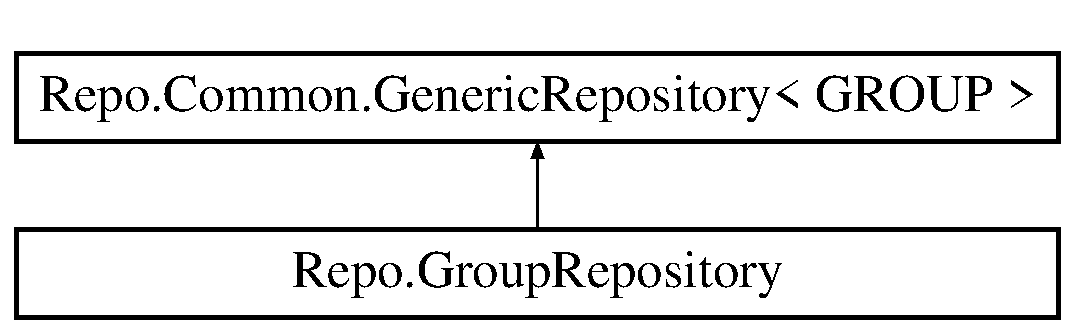
\includegraphics[height=2.000000cm]{class_repo_1_1_group_repository}
\end{center}
\end{figure}
\subsection*{Public Member Functions}
\begin{DoxyCompactItemize}
\item 
\hyperlink{class_repo_1_1_group_repository_a0bc17bb5ba1e4129530362ed1b0fd744}{Group\+Repository} (Db\+Context context)
\end{DoxyCompactItemize}
\subsection*{Additional Inherited Members}


\subsection{Constructor \& Destructor Documentation}
\mbox{\Hypertarget{class_repo_1_1_group_repository_a0bc17bb5ba1e4129530362ed1b0fd744}\label{class_repo_1_1_group_repository_a0bc17bb5ba1e4129530362ed1b0fd744}} 
\index{Repo\+::\+Group\+Repository@{Repo\+::\+Group\+Repository}!Group\+Repository@{Group\+Repository}}
\index{Group\+Repository@{Group\+Repository}!Repo\+::\+Group\+Repository@{Repo\+::\+Group\+Repository}}
\subsubsection{\texorpdfstring{Group\+Repository()}{GroupRepository()}}
{\footnotesize\ttfamily Repo.\+Group\+Repository.\+Group\+Repository (\begin{DoxyParamCaption}\item[{Db\+Context}]{context }\end{DoxyParamCaption})}



The documentation for this class was generated from the following file\+:\begin{DoxyCompactItemize}
\item 
D\+:/\+\_\+\+W\+O\+R\+K/\+\_\+\+S\+T\+E\+P/\+In\+Study\+Asp/\+Repo/\hyperlink{_group_repository_8cs}{Group\+Repository.\+cs}\end{DoxyCompactItemize}

\hypertarget{class_in_study_asp_1_1_controllers_1_1_home_controller}{}\section{In\+Study\+Asp.\+Controllers.\+Home\+Controller Class Reference}
\label{class_in_study_asp_1_1_controllers_1_1_home_controller}\index{In\+Study\+Asp.\+Controllers.\+Home\+Controller@{In\+Study\+Asp.\+Controllers.\+Home\+Controller}}
Inheritance diagram for In\+Study\+Asp.\+Controllers.\+Home\+Controller\+:\begin{figure}[H]
\begin{center}
\leavevmode
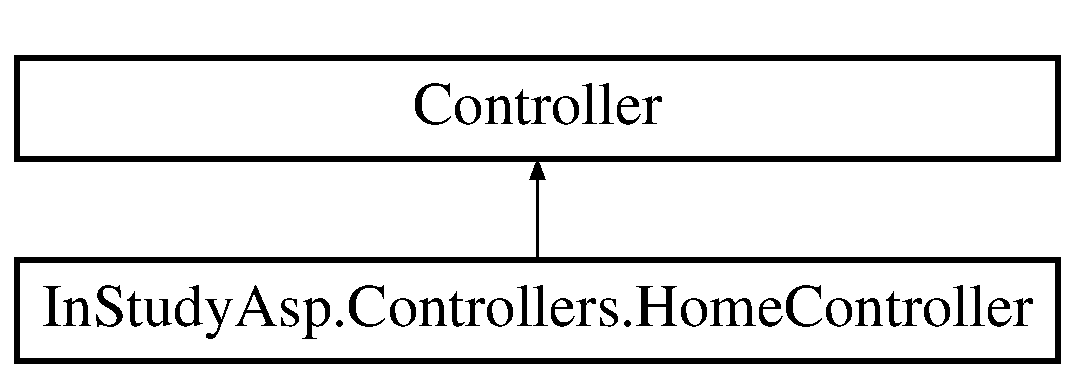
\includegraphics[height=2.000000cm]{class_in_study_asp_1_1_controllers_1_1_home_controller}
\end{center}
\end{figure}
\subsection*{Public Member Functions}
\begin{DoxyCompactItemize}
\item 
Action\+Result \hyperlink{class_in_study_asp_1_1_controllers_1_1_home_controller_a15eec3973e09a36299920ddd2a4af067}{Index} ()
\end{DoxyCompactItemize}


\subsection{Member Function Documentation}
\mbox{\Hypertarget{class_in_study_asp_1_1_controllers_1_1_home_controller_a15eec3973e09a36299920ddd2a4af067}\label{class_in_study_asp_1_1_controllers_1_1_home_controller_a15eec3973e09a36299920ddd2a4af067}} 
\index{In\+Study\+Asp\+::\+Controllers\+::\+Home\+Controller@{In\+Study\+Asp\+::\+Controllers\+::\+Home\+Controller}!Index@{Index}}
\index{Index@{Index}!In\+Study\+Asp\+::\+Controllers\+::\+Home\+Controller@{In\+Study\+Asp\+::\+Controllers\+::\+Home\+Controller}}
\subsubsection{\texorpdfstring{Index()}{Index()}}
{\footnotesize\ttfamily Action\+Result In\+Study\+Asp.\+Controllers.\+Home\+Controller.\+Index (\begin{DoxyParamCaption}{ }\end{DoxyParamCaption})}



The documentation for this class was generated from the following file\+:\begin{DoxyCompactItemize}
\item 
D\+:/\+\_\+\+W\+O\+R\+K/\+\_\+\+S\+T\+E\+P/\+In\+Study\+Asp/\+In\+Study\+Asp/\+Controllers/\hyperlink{_home_controller_8cs}{Home\+Controller.\+cs}\end{DoxyCompactItemize}

\hypertarget{interface_repo_1_1_common_1_1_i_generic_repository}{}\section{Repo.\+Common.\+I\+Generic\+Repository$<$ T $>$ Interface Template Reference}
\label{interface_repo_1_1_common_1_1_i_generic_repository}\index{Repo.\+Common.\+I\+Generic\+Repository$<$ T $>$@{Repo.\+Common.\+I\+Generic\+Repository$<$ T $>$}}
Inheritance diagram for Repo.\+Common.\+I\+Generic\+Repository$<$ T $>$\+:\begin{figure}[H]
\begin{center}
\leavevmode
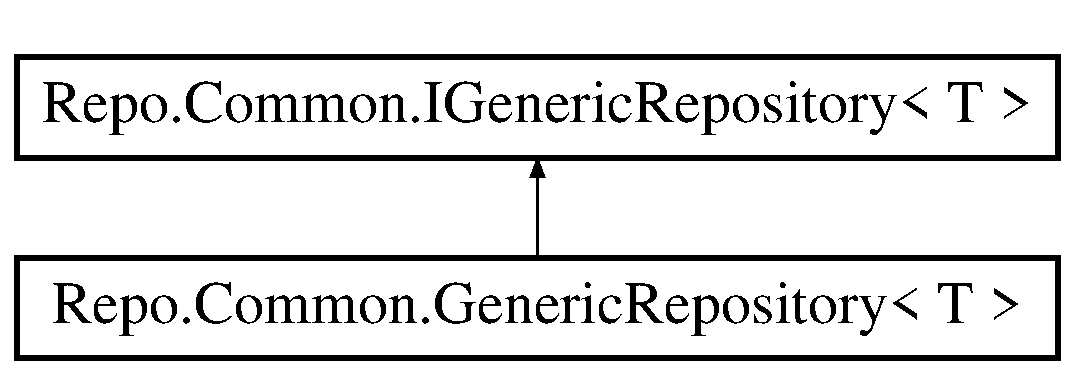
\includegraphics[height=2.000000cm]{interface_repo_1_1_common_1_1_i_generic_repository}
\end{center}
\end{figure}
\subsection*{Public Member Functions}
\begin{DoxyCompactItemize}
\item 
I\+Enumerable$<$ T $>$ \hyperlink{interface_repo_1_1_common_1_1_i_generic_repository_a1ca337e6dced734d843e6955bc997ed0}{Get\+All} ()
\item 
T \hyperlink{interface_repo_1_1_common_1_1_i_generic_repository_acd283f18d8c2a73c52fa49601346e51d}{Get} (int Id)
\item 
I\+Enumerable$<$ T $>$ \hyperlink{interface_repo_1_1_common_1_1_i_generic_repository_a4335770c876a0343a68d6a38f57f67ad}{Find\+By} (Expression$<$ Func$<$ T, bool $>$$>$ predicate)
\item 
void \hyperlink{interface_repo_1_1_common_1_1_i_generic_repository_aaba8a577e9c5b3ae8e86b03b1d94b0f8}{Add\+Or\+Update} (T entity)
\item 
void \hyperlink{interface_repo_1_1_common_1_1_i_generic_repository_a20e38f766023a37a974d33b9b5bffd72}{Delete} (T entity)
\item 
void \hyperlink{interface_repo_1_1_common_1_1_i_generic_repository_aff4307598aa9e4115d3baa2067d67647}{Save} ()
\end{DoxyCompactItemize}


\subsection{Member Function Documentation}
\mbox{\Hypertarget{interface_repo_1_1_common_1_1_i_generic_repository_aaba8a577e9c5b3ae8e86b03b1d94b0f8}\label{interface_repo_1_1_common_1_1_i_generic_repository_aaba8a577e9c5b3ae8e86b03b1d94b0f8}} 
\index{Repo\+::\+Common\+::\+I\+Generic\+Repository@{Repo\+::\+Common\+::\+I\+Generic\+Repository}!Add\+Or\+Update@{Add\+Or\+Update}}
\index{Add\+Or\+Update@{Add\+Or\+Update}!Repo\+::\+Common\+::\+I\+Generic\+Repository@{Repo\+::\+Common\+::\+I\+Generic\+Repository}}
\subsubsection{\texorpdfstring{Add\+Or\+Update()}{AddOrUpdate()}}
{\footnotesize\ttfamily void \hyperlink{interface_repo_1_1_common_1_1_i_generic_repository}{Repo.\+Common.\+I\+Generic\+Repository}$<$ T $>$.Add\+Or\+Update (\begin{DoxyParamCaption}\item[{T}]{entity }\end{DoxyParamCaption})}



Implemented in \hyperlink{class_repo_1_1_common_1_1_generic_repository_a2370df477136ac65eacb282af1d00a9c}{Repo.\+Common.\+Generic\+Repository$<$ T $>$}.

\mbox{\Hypertarget{interface_repo_1_1_common_1_1_i_generic_repository_a20e38f766023a37a974d33b9b5bffd72}\label{interface_repo_1_1_common_1_1_i_generic_repository_a20e38f766023a37a974d33b9b5bffd72}} 
\index{Repo\+::\+Common\+::\+I\+Generic\+Repository@{Repo\+::\+Common\+::\+I\+Generic\+Repository}!Delete@{Delete}}
\index{Delete@{Delete}!Repo\+::\+Common\+::\+I\+Generic\+Repository@{Repo\+::\+Common\+::\+I\+Generic\+Repository}}
\subsubsection{\texorpdfstring{Delete()}{Delete()}}
{\footnotesize\ttfamily void \hyperlink{interface_repo_1_1_common_1_1_i_generic_repository}{Repo.\+Common.\+I\+Generic\+Repository}$<$ T $>$.Delete (\begin{DoxyParamCaption}\item[{T}]{entity }\end{DoxyParamCaption})}



Implemented in \hyperlink{class_repo_1_1_common_1_1_generic_repository_a9714e5c61c4f3541137bb83bebe054bb}{Repo.\+Common.\+Generic\+Repository$<$ T $>$}.

\mbox{\Hypertarget{interface_repo_1_1_common_1_1_i_generic_repository_a4335770c876a0343a68d6a38f57f67ad}\label{interface_repo_1_1_common_1_1_i_generic_repository_a4335770c876a0343a68d6a38f57f67ad}} 
\index{Repo\+::\+Common\+::\+I\+Generic\+Repository@{Repo\+::\+Common\+::\+I\+Generic\+Repository}!Find\+By@{Find\+By}}
\index{Find\+By@{Find\+By}!Repo\+::\+Common\+::\+I\+Generic\+Repository@{Repo\+::\+Common\+::\+I\+Generic\+Repository}}
\subsubsection{\texorpdfstring{Find\+By()}{FindBy()}}
{\footnotesize\ttfamily I\+Enumerable$<$T$>$ \hyperlink{interface_repo_1_1_common_1_1_i_generic_repository}{Repo.\+Common.\+I\+Generic\+Repository}$<$ T $>$.Find\+By (\begin{DoxyParamCaption}\item[{Expression$<$ Func$<$ T, bool $>$$>$}]{predicate }\end{DoxyParamCaption})}

\mbox{\Hypertarget{interface_repo_1_1_common_1_1_i_generic_repository_acd283f18d8c2a73c52fa49601346e51d}\label{interface_repo_1_1_common_1_1_i_generic_repository_acd283f18d8c2a73c52fa49601346e51d}} 
\index{Repo\+::\+Common\+::\+I\+Generic\+Repository@{Repo\+::\+Common\+::\+I\+Generic\+Repository}!Get@{Get}}
\index{Get@{Get}!Repo\+::\+Common\+::\+I\+Generic\+Repository@{Repo\+::\+Common\+::\+I\+Generic\+Repository}}
\subsubsection{\texorpdfstring{Get()}{Get()}}
{\footnotesize\ttfamily T \hyperlink{interface_repo_1_1_common_1_1_i_generic_repository}{Repo.\+Common.\+I\+Generic\+Repository}$<$ T $>$.Get (\begin{DoxyParamCaption}\item[{int}]{Id }\end{DoxyParamCaption})}



Implemented in \hyperlink{class_repo_1_1_common_1_1_generic_repository_ac3f609e57fb59eee8b0d8aaf2d1dd220}{Repo.\+Common.\+Generic\+Repository$<$ T $>$}.

\mbox{\Hypertarget{interface_repo_1_1_common_1_1_i_generic_repository_a1ca337e6dced734d843e6955bc997ed0}\label{interface_repo_1_1_common_1_1_i_generic_repository_a1ca337e6dced734d843e6955bc997ed0}} 
\index{Repo\+::\+Common\+::\+I\+Generic\+Repository@{Repo\+::\+Common\+::\+I\+Generic\+Repository}!Get\+All@{Get\+All}}
\index{Get\+All@{Get\+All}!Repo\+::\+Common\+::\+I\+Generic\+Repository@{Repo\+::\+Common\+::\+I\+Generic\+Repository}}
\subsubsection{\texorpdfstring{Get\+All()}{GetAll()}}
{\footnotesize\ttfamily I\+Enumerable$<$T$>$ \hyperlink{interface_repo_1_1_common_1_1_i_generic_repository}{Repo.\+Common.\+I\+Generic\+Repository}$<$ T $>$.Get\+All (\begin{DoxyParamCaption}{ }\end{DoxyParamCaption})}



Implemented in \hyperlink{class_repo_1_1_common_1_1_generic_repository_a819ba9c87b3246d17672f348c2162c7f}{Repo.\+Common.\+Generic\+Repository$<$ T $>$}.

\mbox{\Hypertarget{interface_repo_1_1_common_1_1_i_generic_repository_aff4307598aa9e4115d3baa2067d67647}\label{interface_repo_1_1_common_1_1_i_generic_repository_aff4307598aa9e4115d3baa2067d67647}} 
\index{Repo\+::\+Common\+::\+I\+Generic\+Repository@{Repo\+::\+Common\+::\+I\+Generic\+Repository}!Save@{Save}}
\index{Save@{Save}!Repo\+::\+Common\+::\+I\+Generic\+Repository@{Repo\+::\+Common\+::\+I\+Generic\+Repository}}
\subsubsection{\texorpdfstring{Save()}{Save()}}
{\footnotesize\ttfamily void \hyperlink{interface_repo_1_1_common_1_1_i_generic_repository}{Repo.\+Common.\+I\+Generic\+Repository}$<$ T $>$.Save (\begin{DoxyParamCaption}{ }\end{DoxyParamCaption})}



Implemented in \hyperlink{class_repo_1_1_common_1_1_generic_repository_ab66ace5b2cc69867ce37dc996fc6c6e8}{Repo.\+Common.\+Generic\+Repository$<$ T $>$}.



The documentation for this interface was generated from the following file\+:\begin{DoxyCompactItemize}
\item 
D\+:/\+\_\+\+W\+O\+R\+K/\+\_\+\+S\+T\+E\+P/\+In\+Study\+Asp/\+Repo/\+Common/\hyperlink{_i_generic_repository_8cs}{I\+Generic\+Repository.\+cs}\end{DoxyCompactItemize}

\hypertarget{class_in_study_asp_1_1_mvc_application}{}\section{In\+Study\+Asp.\+Mvc\+Application Class Reference}
\label{class_in_study_asp_1_1_mvc_application}\index{In\+Study\+Asp.\+Mvc\+Application@{In\+Study\+Asp.\+Mvc\+Application}}
Inheritance diagram for In\+Study\+Asp.\+Mvc\+Application\+:\begin{figure}[H]
\begin{center}
\leavevmode
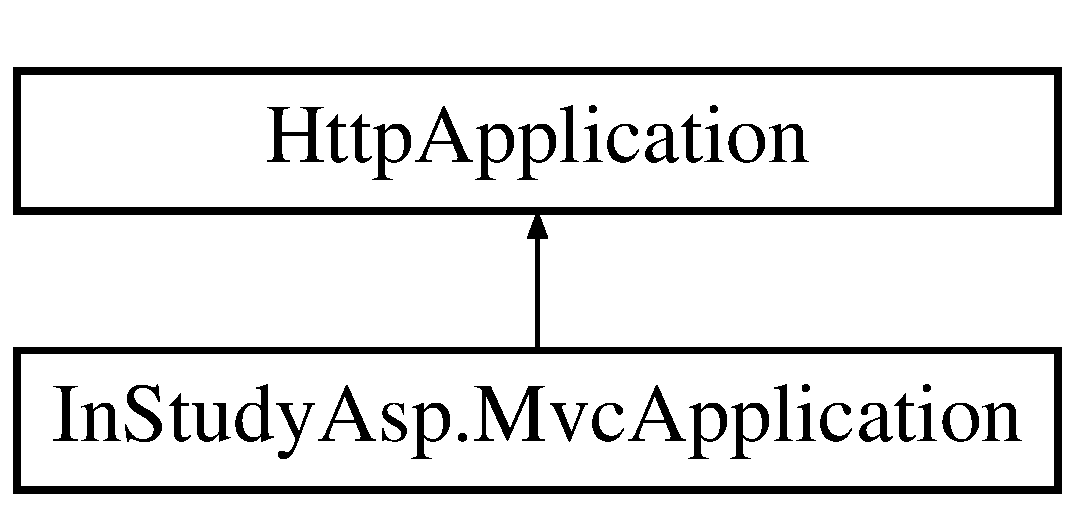
\includegraphics[height=2.000000cm]{class_in_study_asp_1_1_mvc_application}
\end{center}
\end{figure}
\subsection*{Protected Member Functions}
\begin{DoxyCompactItemize}
\item 
void \hyperlink{class_in_study_asp_1_1_mvc_application_aa30bba9d99d413301ced2c1fe641ab7a}{Application\+\_\+\+Start} ()
\end{DoxyCompactItemize}


\subsection{Member Function Documentation}
\mbox{\Hypertarget{class_in_study_asp_1_1_mvc_application_aa30bba9d99d413301ced2c1fe641ab7a}\label{class_in_study_asp_1_1_mvc_application_aa30bba9d99d413301ced2c1fe641ab7a}} 
\index{In\+Study\+Asp\+::\+Mvc\+Application@{In\+Study\+Asp\+::\+Mvc\+Application}!Application\+\_\+\+Start@{Application\+\_\+\+Start}}
\index{Application\+\_\+\+Start@{Application\+\_\+\+Start}!In\+Study\+Asp\+::\+Mvc\+Application@{In\+Study\+Asp\+::\+Mvc\+Application}}
\subsubsection{\texorpdfstring{Application\+\_\+\+Start()}{Application\_Start()}}
{\footnotesize\ttfamily void In\+Study\+Asp.\+Mvc\+Application.\+Application\+\_\+\+Start (\begin{DoxyParamCaption}{ }\end{DoxyParamCaption})\hspace{0.3cm}{\ttfamily [protected]}}



The documentation for this class was generated from the following file\+:\begin{DoxyCompactItemize}
\item 
D\+:/\+\_\+\+W\+O\+R\+K/\+\_\+\+S\+T\+E\+P/\+In\+Study\+Asp/\+In\+Study\+Asp/\hyperlink{_global_8asax_8cs}{Global.\+asax.\+cs}\end{DoxyCompactItemize}

\hypertarget{class_in_study_asp_1_1_app___start_1_1_ninject_web_common}{}\section{In\+Study\+Asp.\+App\+\_\+\+Start.\+Ninject\+Web\+Common Class Reference}
\label{class_in_study_asp_1_1_app___start_1_1_ninject_web_common}\index{In\+Study\+Asp.\+App\+\_\+\+Start.\+Ninject\+Web\+Common@{In\+Study\+Asp.\+App\+\_\+\+Start.\+Ninject\+Web\+Common}}
\subsection*{Static Public Member Functions}
\begin{DoxyCompactItemize}
\item 
static void \hyperlink{class_in_study_asp_1_1_app___start_1_1_ninject_web_common_a5f2fd0336cc58d1bff7e9bacaf3dac0f}{Start} ()
\begin{DoxyCompactList}\small\item\em Starts the application \end{DoxyCompactList}\item 
static void \hyperlink{class_in_study_asp_1_1_app___start_1_1_ninject_web_common_a61ec74f8d4223f5fa02c43d6cd92559c}{Stop} ()
\begin{DoxyCompactList}\small\item\em Stops the application. \end{DoxyCompactList}\end{DoxyCompactItemize}
\subsection*{Static Private Member Functions}
\begin{DoxyCompactItemize}
\item 
static I\+Kernel \hyperlink{class_in_study_asp_1_1_app___start_1_1_ninject_web_common_ada95e960047d598b69e9aac859977a35}{Create\+Kernel} ()
\begin{DoxyCompactList}\small\item\em Creates the kernel that will manage your application. \end{DoxyCompactList}\item 
static void \hyperlink{class_in_study_asp_1_1_app___start_1_1_ninject_web_common_a6ef77a66355b50bbe2f357776e14ffa1}{Register\+Services} (I\+Kernel kernel)
\begin{DoxyCompactList}\small\item\em Load your modules or register your services here! \end{DoxyCompactList}\end{DoxyCompactItemize}
\subsection*{Static Private Attributes}
\begin{DoxyCompactItemize}
\item 
static readonly Bootstrapper \hyperlink{class_in_study_asp_1_1_app___start_1_1_ninject_web_common_ae16416703e3d7ba27646e2d8c317244b}{bootstrapper} = new Bootstrapper()
\end{DoxyCompactItemize}


\subsection{Member Function Documentation}
\mbox{\Hypertarget{class_in_study_asp_1_1_app___start_1_1_ninject_web_common_ada95e960047d598b69e9aac859977a35}\label{class_in_study_asp_1_1_app___start_1_1_ninject_web_common_ada95e960047d598b69e9aac859977a35}} 
\index{In\+Study\+Asp\+::\+App\+\_\+\+Start\+::\+Ninject\+Web\+Common@{In\+Study\+Asp\+::\+App\+\_\+\+Start\+::\+Ninject\+Web\+Common}!Create\+Kernel@{Create\+Kernel}}
\index{Create\+Kernel@{Create\+Kernel}!In\+Study\+Asp\+::\+App\+\_\+\+Start\+::\+Ninject\+Web\+Common@{In\+Study\+Asp\+::\+App\+\_\+\+Start\+::\+Ninject\+Web\+Common}}
\subsubsection{\texorpdfstring{Create\+Kernel()}{CreateKernel()}}
{\footnotesize\ttfamily static I\+Kernel In\+Study\+Asp.\+App\+\_\+\+Start.\+Ninject\+Web\+Common.\+Create\+Kernel (\begin{DoxyParamCaption}{ }\end{DoxyParamCaption})\hspace{0.3cm}{\ttfamily [static]}, {\ttfamily [private]}}



Creates the kernel that will manage your application. 

\begin{DoxyReturn}{Returns}
The created kernel.
\end{DoxyReturn}
\mbox{\Hypertarget{class_in_study_asp_1_1_app___start_1_1_ninject_web_common_a6ef77a66355b50bbe2f357776e14ffa1}\label{class_in_study_asp_1_1_app___start_1_1_ninject_web_common_a6ef77a66355b50bbe2f357776e14ffa1}} 
\index{In\+Study\+Asp\+::\+App\+\_\+\+Start\+::\+Ninject\+Web\+Common@{In\+Study\+Asp\+::\+App\+\_\+\+Start\+::\+Ninject\+Web\+Common}!Register\+Services@{Register\+Services}}
\index{Register\+Services@{Register\+Services}!In\+Study\+Asp\+::\+App\+\_\+\+Start\+::\+Ninject\+Web\+Common@{In\+Study\+Asp\+::\+App\+\_\+\+Start\+::\+Ninject\+Web\+Common}}
\subsubsection{\texorpdfstring{Register\+Services()}{RegisterServices()}}
{\footnotesize\ttfamily static void In\+Study\+Asp.\+App\+\_\+\+Start.\+Ninject\+Web\+Common.\+Register\+Services (\begin{DoxyParamCaption}\item[{I\+Kernel}]{kernel }\end{DoxyParamCaption})\hspace{0.3cm}{\ttfamily [static]}, {\ttfamily [private]}}



Load your modules or register your services here! 


\begin{DoxyParams}{Parameters}
{\em kernel} & The kernel.\\
\hline
\end{DoxyParams}
\mbox{\Hypertarget{class_in_study_asp_1_1_app___start_1_1_ninject_web_common_a5f2fd0336cc58d1bff7e9bacaf3dac0f}\label{class_in_study_asp_1_1_app___start_1_1_ninject_web_common_a5f2fd0336cc58d1bff7e9bacaf3dac0f}} 
\index{In\+Study\+Asp\+::\+App\+\_\+\+Start\+::\+Ninject\+Web\+Common@{In\+Study\+Asp\+::\+App\+\_\+\+Start\+::\+Ninject\+Web\+Common}!Start@{Start}}
\index{Start@{Start}!In\+Study\+Asp\+::\+App\+\_\+\+Start\+::\+Ninject\+Web\+Common@{In\+Study\+Asp\+::\+App\+\_\+\+Start\+::\+Ninject\+Web\+Common}}
\subsubsection{\texorpdfstring{Start()}{Start()}}
{\footnotesize\ttfamily static void In\+Study\+Asp.\+App\+\_\+\+Start.\+Ninject\+Web\+Common.\+Start (\begin{DoxyParamCaption}{ }\end{DoxyParamCaption})\hspace{0.3cm}{\ttfamily [static]}}



Starts the application 

\mbox{\Hypertarget{class_in_study_asp_1_1_app___start_1_1_ninject_web_common_a61ec74f8d4223f5fa02c43d6cd92559c}\label{class_in_study_asp_1_1_app___start_1_1_ninject_web_common_a61ec74f8d4223f5fa02c43d6cd92559c}} 
\index{In\+Study\+Asp\+::\+App\+\_\+\+Start\+::\+Ninject\+Web\+Common@{In\+Study\+Asp\+::\+App\+\_\+\+Start\+::\+Ninject\+Web\+Common}!Stop@{Stop}}
\index{Stop@{Stop}!In\+Study\+Asp\+::\+App\+\_\+\+Start\+::\+Ninject\+Web\+Common@{In\+Study\+Asp\+::\+App\+\_\+\+Start\+::\+Ninject\+Web\+Common}}
\subsubsection{\texorpdfstring{Stop()}{Stop()}}
{\footnotesize\ttfamily static void In\+Study\+Asp.\+App\+\_\+\+Start.\+Ninject\+Web\+Common.\+Stop (\begin{DoxyParamCaption}{ }\end{DoxyParamCaption})\hspace{0.3cm}{\ttfamily [static]}}



Stops the application. 



\subsection{Member Data Documentation}
\mbox{\Hypertarget{class_in_study_asp_1_1_app___start_1_1_ninject_web_common_ae16416703e3d7ba27646e2d8c317244b}\label{class_in_study_asp_1_1_app___start_1_1_ninject_web_common_ae16416703e3d7ba27646e2d8c317244b}} 
\index{In\+Study\+Asp\+::\+App\+\_\+\+Start\+::\+Ninject\+Web\+Common@{In\+Study\+Asp\+::\+App\+\_\+\+Start\+::\+Ninject\+Web\+Common}!bootstrapper@{bootstrapper}}
\index{bootstrapper@{bootstrapper}!In\+Study\+Asp\+::\+App\+\_\+\+Start\+::\+Ninject\+Web\+Common@{In\+Study\+Asp\+::\+App\+\_\+\+Start\+::\+Ninject\+Web\+Common}}
\subsubsection{\texorpdfstring{bootstrapper}{bootstrapper}}
{\footnotesize\ttfamily readonly Bootstrapper In\+Study\+Asp.\+App\+\_\+\+Start.\+Ninject\+Web\+Common.\+bootstrapper = new Bootstrapper()\hspace{0.3cm}{\ttfamily [static]}, {\ttfamily [private]}}



The documentation for this class was generated from the following file\+:\begin{DoxyCompactItemize}
\item 
D\+:/\+\_\+\+W\+O\+R\+K/\+\_\+\+S\+T\+E\+P/\+In\+Study\+Asp/\+In\+Study\+Asp/\+App\+\_\+\+Start/\hyperlink{_ninject_web_common_8cs}{Ninject\+Web\+Common.\+cs}\end{DoxyCompactItemize}

\hypertarget{class_in_study_asp_1_1_route_config}{}\section{In\+Study\+Asp.\+Route\+Config Class Reference}
\label{class_in_study_asp_1_1_route_config}\index{In\+Study\+Asp.\+Route\+Config@{In\+Study\+Asp.\+Route\+Config}}
\subsection*{Static Public Member Functions}
\begin{DoxyCompactItemize}
\item 
static void \hyperlink{class_in_study_asp_1_1_route_config_a3fc41a6de193b638a62c47244aa87b7e}{Register\+Routes} (Route\+Collection routes)
\end{DoxyCompactItemize}


\subsection{Member Function Documentation}
\mbox{\Hypertarget{class_in_study_asp_1_1_route_config_a3fc41a6de193b638a62c47244aa87b7e}\label{class_in_study_asp_1_1_route_config_a3fc41a6de193b638a62c47244aa87b7e}} 
\index{In\+Study\+Asp\+::\+Route\+Config@{In\+Study\+Asp\+::\+Route\+Config}!Register\+Routes@{Register\+Routes}}
\index{Register\+Routes@{Register\+Routes}!In\+Study\+Asp\+::\+Route\+Config@{In\+Study\+Asp\+::\+Route\+Config}}
\subsubsection{\texorpdfstring{Register\+Routes()}{RegisterRoutes()}}
{\footnotesize\ttfamily static void In\+Study\+Asp.\+Route\+Config.\+Register\+Routes (\begin{DoxyParamCaption}\item[{Route\+Collection}]{routes }\end{DoxyParamCaption})\hspace{0.3cm}{\ttfamily [static]}}



The documentation for this class was generated from the following file\+:\begin{DoxyCompactItemize}
\item 
D\+:/\+\_\+\+W\+O\+R\+K/\+\_\+\+S\+T\+E\+P/\+In\+Study\+Asp/\+In\+Study\+Asp/\+App\+\_\+\+Start/\hyperlink{_route_config_8cs}{Route\+Config.\+cs}\end{DoxyCompactItemize}

\hypertarget{class_e_f_oracle_1_1_model_1_1_s_c_h_e_d_u_l_e}{}\section{E\+F\+Oracle.\+Model.\+S\+C\+H\+E\+D\+U\+LE Class Reference}
\label{class_e_f_oracle_1_1_model_1_1_s_c_h_e_d_u_l_e}\index{E\+F\+Oracle.\+Model.\+S\+C\+H\+E\+D\+U\+LE@{E\+F\+Oracle.\+Model.\+S\+C\+H\+E\+D\+U\+LE}}


Specifying view metadata for \hyperlink{class_e_f_oracle_1_1_model_1_1_s_c_h_e_d_u_l_e}{S\+C\+H\+E\+D\+U\+LE} class.  


Inheritance diagram for E\+F\+Oracle.\+Model.\+S\+C\+H\+E\+D\+U\+LE\+:\begin{figure}[H]
\begin{center}
\leavevmode
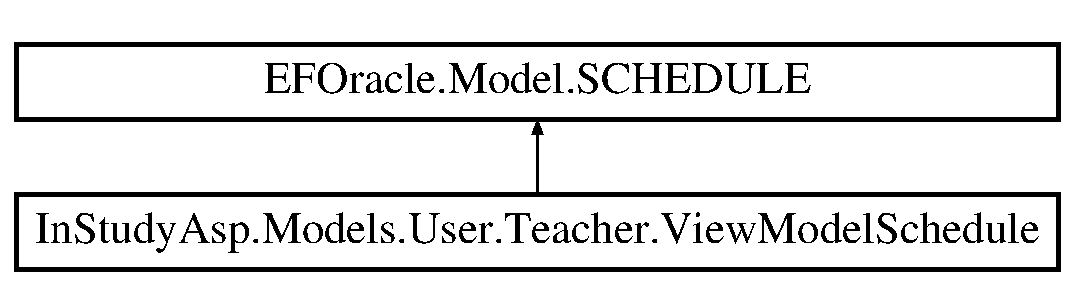
\includegraphics[height=2.000000cm]{class_e_f_oracle_1_1_model_1_1_s_c_h_e_d_u_l_e}
\end{center}
\end{figure}
\subsection*{Properties}
\begin{DoxyCompactItemize}
\item 
decimal \hyperlink{class_e_f_oracle_1_1_model_1_1_s_c_h_e_d_u_l_e_a68935d61b8eb7170cd88d9d90b803b05}{T\+E\+A\+C\+H\+E\+R\+\_\+\+ID}\hspace{0.3cm}{\ttfamily  \mbox{[}get, set\mbox{]}}
\item 
string \hyperlink{class_e_f_oracle_1_1_model_1_1_s_c_h_e_d_u_l_e_aa0b33a5dbbf6c590afd18a5589e5427f}{G\+R\+O\+U\+P\+\_\+\+C\+O\+DE}\hspace{0.3cm}{\ttfamily  \mbox{[}get, set\mbox{]}}
\item 
decimal \hyperlink{class_e_f_oracle_1_1_model_1_1_s_c_h_e_d_u_l_e_ac6a505dacf6cc2d8575672f1041a68f7}{D\+I\+S\+C\+I\+P\+L\+I\+N\+E\+\_\+\+C\+O\+DE}\hspace{0.3cm}{\ttfamily  \mbox{[}get, set\mbox{]}}
\item 
Date\+Time \hyperlink{class_e_f_oracle_1_1_model_1_1_s_c_h_e_d_u_l_e_ae7a440479613292131125de6422126ed}{S\+C\+H\+E\+D\+U\+L\+E\+\_\+\+D\+A\+TE}\hspace{0.3cm}{\ttfamily  \mbox{[}get, set\mbox{]}}
\item 
decimal \hyperlink{class_e_f_oracle_1_1_model_1_1_s_c_h_e_d_u_l_e_abeac12f973abfb2f7811b88680e480b1}{S\+C\+H\+E\+D\+U\+L\+E\+\_\+\+R\+O\+OM}\hspace{0.3cm}{\ttfamily  \mbox{[}get, set\mbox{]}}
\item 
virtual \hyperlink{class_e_f_oracle_1_1_model_1_1_d_i_s_c_i_p_l_i_n_e}{D\+I\+S\+C\+I\+P\+L\+I\+NE} \hyperlink{class_e_f_oracle_1_1_model_1_1_s_c_h_e_d_u_l_e_abd6e267b33f3d63e1ebcf0f669da66f1}{D\+I\+S\+C\+I\+P\+L\+I\+NE}\hspace{0.3cm}{\ttfamily  \mbox{[}get, set\mbox{]}}
\item 
virtual \hyperlink{class_e_f_oracle_1_1_model_1_1_g_r_o_u_p}{G\+R\+O\+UP} \hyperlink{class_e_f_oracle_1_1_model_1_1_s_c_h_e_d_u_l_e_a5d9abb16390ba4706d7e38dda10f51ce}{G\+R\+O\+UP}\hspace{0.3cm}{\ttfamily  \mbox{[}get, set\mbox{]}}
\item 
virtual \hyperlink{class_e_f_oracle_1_1_model_1_1_t_e_a_c_h_e_r}{T\+E\+A\+C\+H\+ER} \hyperlink{class_e_f_oracle_1_1_model_1_1_s_c_h_e_d_u_l_e_ac72f394cae43d132907b123022a6006e}{T\+E\+A\+C\+H\+ER}\hspace{0.3cm}{\ttfamily  \mbox{[}get, set\mbox{]}}
\end{DoxyCompactItemize}


\subsection{Detailed Description}
Specifying view metadata for \hyperlink{class_e_f_oracle_1_1_model_1_1_s_c_h_e_d_u_l_e}{S\+C\+H\+E\+D\+U\+LE} class. 

\subsection{Property Documentation}
\mbox{\Hypertarget{class_e_f_oracle_1_1_model_1_1_s_c_h_e_d_u_l_e_abd6e267b33f3d63e1ebcf0f669da66f1}\label{class_e_f_oracle_1_1_model_1_1_s_c_h_e_d_u_l_e_abd6e267b33f3d63e1ebcf0f669da66f1}} 
\index{E\+F\+Oracle\+::\+Model\+::\+S\+C\+H\+E\+D\+U\+LE@{E\+F\+Oracle\+::\+Model\+::\+S\+C\+H\+E\+D\+U\+LE}!D\+I\+S\+C\+I\+P\+L\+I\+NE@{D\+I\+S\+C\+I\+P\+L\+I\+NE}}
\index{D\+I\+S\+C\+I\+P\+L\+I\+NE@{D\+I\+S\+C\+I\+P\+L\+I\+NE}!E\+F\+Oracle\+::\+Model\+::\+S\+C\+H\+E\+D\+U\+LE@{E\+F\+Oracle\+::\+Model\+::\+S\+C\+H\+E\+D\+U\+LE}}
\subsubsection{\texorpdfstring{D\+I\+S\+C\+I\+P\+L\+I\+NE}{DISCIPLINE}}
{\footnotesize\ttfamily virtual \hyperlink{class_e_f_oracle_1_1_model_1_1_d_i_s_c_i_p_l_i_n_e}{D\+I\+S\+C\+I\+P\+L\+I\+NE} E\+F\+Oracle.\+Model.\+S\+C\+H\+E\+D\+U\+L\+E.\+D\+I\+S\+C\+I\+P\+L\+I\+NE\hspace{0.3cm}{\ttfamily [get]}, {\ttfamily [set]}}

\mbox{\Hypertarget{class_e_f_oracle_1_1_model_1_1_s_c_h_e_d_u_l_e_ac6a505dacf6cc2d8575672f1041a68f7}\label{class_e_f_oracle_1_1_model_1_1_s_c_h_e_d_u_l_e_ac6a505dacf6cc2d8575672f1041a68f7}} 
\index{E\+F\+Oracle\+::\+Model\+::\+S\+C\+H\+E\+D\+U\+LE@{E\+F\+Oracle\+::\+Model\+::\+S\+C\+H\+E\+D\+U\+LE}!D\+I\+S\+C\+I\+P\+L\+I\+N\+E\+\_\+\+C\+O\+DE@{D\+I\+S\+C\+I\+P\+L\+I\+N\+E\+\_\+\+C\+O\+DE}}
\index{D\+I\+S\+C\+I\+P\+L\+I\+N\+E\+\_\+\+C\+O\+DE@{D\+I\+S\+C\+I\+P\+L\+I\+N\+E\+\_\+\+C\+O\+DE}!E\+F\+Oracle\+::\+Model\+::\+S\+C\+H\+E\+D\+U\+LE@{E\+F\+Oracle\+::\+Model\+::\+S\+C\+H\+E\+D\+U\+LE}}
\subsubsection{\texorpdfstring{D\+I\+S\+C\+I\+P\+L\+I\+N\+E\+\_\+\+C\+O\+DE}{DISCIPLINE\_CODE}}
{\footnotesize\ttfamily decimal E\+F\+Oracle.\+Model.\+S\+C\+H\+E\+D\+U\+L\+E.\+D\+I\+S\+C\+I\+P\+L\+I\+N\+E\+\_\+\+C\+O\+DE\hspace{0.3cm}{\ttfamily [get]}, {\ttfamily [set]}}

\mbox{\Hypertarget{class_e_f_oracle_1_1_model_1_1_s_c_h_e_d_u_l_e_a5d9abb16390ba4706d7e38dda10f51ce}\label{class_e_f_oracle_1_1_model_1_1_s_c_h_e_d_u_l_e_a5d9abb16390ba4706d7e38dda10f51ce}} 
\index{E\+F\+Oracle\+::\+Model\+::\+S\+C\+H\+E\+D\+U\+LE@{E\+F\+Oracle\+::\+Model\+::\+S\+C\+H\+E\+D\+U\+LE}!G\+R\+O\+UP@{G\+R\+O\+UP}}
\index{G\+R\+O\+UP@{G\+R\+O\+UP}!E\+F\+Oracle\+::\+Model\+::\+S\+C\+H\+E\+D\+U\+LE@{E\+F\+Oracle\+::\+Model\+::\+S\+C\+H\+E\+D\+U\+LE}}
\subsubsection{\texorpdfstring{G\+R\+O\+UP}{GROUP}}
{\footnotesize\ttfamily virtual \hyperlink{class_e_f_oracle_1_1_model_1_1_g_r_o_u_p}{G\+R\+O\+UP} E\+F\+Oracle.\+Model.\+S\+C\+H\+E\+D\+U\+L\+E.\+G\+R\+O\+UP\hspace{0.3cm}{\ttfamily [get]}, {\ttfamily [set]}}

\mbox{\Hypertarget{class_e_f_oracle_1_1_model_1_1_s_c_h_e_d_u_l_e_aa0b33a5dbbf6c590afd18a5589e5427f}\label{class_e_f_oracle_1_1_model_1_1_s_c_h_e_d_u_l_e_aa0b33a5dbbf6c590afd18a5589e5427f}} 
\index{E\+F\+Oracle\+::\+Model\+::\+S\+C\+H\+E\+D\+U\+LE@{E\+F\+Oracle\+::\+Model\+::\+S\+C\+H\+E\+D\+U\+LE}!G\+R\+O\+U\+P\+\_\+\+C\+O\+DE@{G\+R\+O\+U\+P\+\_\+\+C\+O\+DE}}
\index{G\+R\+O\+U\+P\+\_\+\+C\+O\+DE@{G\+R\+O\+U\+P\+\_\+\+C\+O\+DE}!E\+F\+Oracle\+::\+Model\+::\+S\+C\+H\+E\+D\+U\+LE@{E\+F\+Oracle\+::\+Model\+::\+S\+C\+H\+E\+D\+U\+LE}}
\subsubsection{\texorpdfstring{G\+R\+O\+U\+P\+\_\+\+C\+O\+DE}{GROUP\_CODE}}
{\footnotesize\ttfamily string E\+F\+Oracle.\+Model.\+S\+C\+H\+E\+D\+U\+L\+E.\+G\+R\+O\+U\+P\+\_\+\+C\+O\+DE\hspace{0.3cm}{\ttfamily [get]}, {\ttfamily [set]}}

\mbox{\Hypertarget{class_e_f_oracle_1_1_model_1_1_s_c_h_e_d_u_l_e_ae7a440479613292131125de6422126ed}\label{class_e_f_oracle_1_1_model_1_1_s_c_h_e_d_u_l_e_ae7a440479613292131125de6422126ed}} 
\index{E\+F\+Oracle\+::\+Model\+::\+S\+C\+H\+E\+D\+U\+LE@{E\+F\+Oracle\+::\+Model\+::\+S\+C\+H\+E\+D\+U\+LE}!S\+C\+H\+E\+D\+U\+L\+E\+\_\+\+D\+A\+TE@{S\+C\+H\+E\+D\+U\+L\+E\+\_\+\+D\+A\+TE}}
\index{S\+C\+H\+E\+D\+U\+L\+E\+\_\+\+D\+A\+TE@{S\+C\+H\+E\+D\+U\+L\+E\+\_\+\+D\+A\+TE}!E\+F\+Oracle\+::\+Model\+::\+S\+C\+H\+E\+D\+U\+LE@{E\+F\+Oracle\+::\+Model\+::\+S\+C\+H\+E\+D\+U\+LE}}
\subsubsection{\texorpdfstring{S\+C\+H\+E\+D\+U\+L\+E\+\_\+\+D\+A\+TE}{SCHEDULE\_DATE}}
{\footnotesize\ttfamily Date\+Time E\+F\+Oracle.\+Model.\+S\+C\+H\+E\+D\+U\+L\+E.\+S\+C\+H\+E\+D\+U\+L\+E\+\_\+\+D\+A\+TE\hspace{0.3cm}{\ttfamily [get]}, {\ttfamily [set]}}

\mbox{\Hypertarget{class_e_f_oracle_1_1_model_1_1_s_c_h_e_d_u_l_e_abeac12f973abfb2f7811b88680e480b1}\label{class_e_f_oracle_1_1_model_1_1_s_c_h_e_d_u_l_e_abeac12f973abfb2f7811b88680e480b1}} 
\index{E\+F\+Oracle\+::\+Model\+::\+S\+C\+H\+E\+D\+U\+LE@{E\+F\+Oracle\+::\+Model\+::\+S\+C\+H\+E\+D\+U\+LE}!S\+C\+H\+E\+D\+U\+L\+E\+\_\+\+R\+O\+OM@{S\+C\+H\+E\+D\+U\+L\+E\+\_\+\+R\+O\+OM}}
\index{S\+C\+H\+E\+D\+U\+L\+E\+\_\+\+R\+O\+OM@{S\+C\+H\+E\+D\+U\+L\+E\+\_\+\+R\+O\+OM}!E\+F\+Oracle\+::\+Model\+::\+S\+C\+H\+E\+D\+U\+LE@{E\+F\+Oracle\+::\+Model\+::\+S\+C\+H\+E\+D\+U\+LE}}
\subsubsection{\texorpdfstring{S\+C\+H\+E\+D\+U\+L\+E\+\_\+\+R\+O\+OM}{SCHEDULE\_ROOM}}
{\footnotesize\ttfamily decimal E\+F\+Oracle.\+Model.\+S\+C\+H\+E\+D\+U\+L\+E.\+S\+C\+H\+E\+D\+U\+L\+E\+\_\+\+R\+O\+OM\hspace{0.3cm}{\ttfamily [get]}, {\ttfamily [set]}}

\mbox{\Hypertarget{class_e_f_oracle_1_1_model_1_1_s_c_h_e_d_u_l_e_ac72f394cae43d132907b123022a6006e}\label{class_e_f_oracle_1_1_model_1_1_s_c_h_e_d_u_l_e_ac72f394cae43d132907b123022a6006e}} 
\index{E\+F\+Oracle\+::\+Model\+::\+S\+C\+H\+E\+D\+U\+LE@{E\+F\+Oracle\+::\+Model\+::\+S\+C\+H\+E\+D\+U\+LE}!T\+E\+A\+C\+H\+ER@{T\+E\+A\+C\+H\+ER}}
\index{T\+E\+A\+C\+H\+ER@{T\+E\+A\+C\+H\+ER}!E\+F\+Oracle\+::\+Model\+::\+S\+C\+H\+E\+D\+U\+LE@{E\+F\+Oracle\+::\+Model\+::\+S\+C\+H\+E\+D\+U\+LE}}
\subsubsection{\texorpdfstring{T\+E\+A\+C\+H\+ER}{TEACHER}}
{\footnotesize\ttfamily virtual \hyperlink{class_e_f_oracle_1_1_model_1_1_t_e_a_c_h_e_r}{T\+E\+A\+C\+H\+ER} E\+F\+Oracle.\+Model.\+S\+C\+H\+E\+D\+U\+L\+E.\+T\+E\+A\+C\+H\+ER\hspace{0.3cm}{\ttfamily [get]}, {\ttfamily [set]}}

\mbox{\Hypertarget{class_e_f_oracle_1_1_model_1_1_s_c_h_e_d_u_l_e_a68935d61b8eb7170cd88d9d90b803b05}\label{class_e_f_oracle_1_1_model_1_1_s_c_h_e_d_u_l_e_a68935d61b8eb7170cd88d9d90b803b05}} 
\index{E\+F\+Oracle\+::\+Model\+::\+S\+C\+H\+E\+D\+U\+LE@{E\+F\+Oracle\+::\+Model\+::\+S\+C\+H\+E\+D\+U\+LE}!T\+E\+A\+C\+H\+E\+R\+\_\+\+ID@{T\+E\+A\+C\+H\+E\+R\+\_\+\+ID}}
\index{T\+E\+A\+C\+H\+E\+R\+\_\+\+ID@{T\+E\+A\+C\+H\+E\+R\+\_\+\+ID}!E\+F\+Oracle\+::\+Model\+::\+S\+C\+H\+E\+D\+U\+LE@{E\+F\+Oracle\+::\+Model\+::\+S\+C\+H\+E\+D\+U\+LE}}
\subsubsection{\texorpdfstring{T\+E\+A\+C\+H\+E\+R\+\_\+\+ID}{TEACHER\_ID}}
{\footnotesize\ttfamily decimal E\+F\+Oracle.\+Model.\+S\+C\+H\+E\+D\+U\+L\+E.\+T\+E\+A\+C\+H\+E\+R\+\_\+\+ID\hspace{0.3cm}{\ttfamily [get]}, {\ttfamily [set]}}



The documentation for this class was generated from the following file\+:\begin{DoxyCompactItemize}
\item 
D\+:/\+\_\+\+W\+O\+R\+K/\+\_\+\+S\+T\+E\+P/\+In\+Study\+Asp/\+E\+F\+Oracle/\+Model/\+Extended/\hyperlink{_extended_2_s_c_h_e_d_u_l_e_8cs}{S\+C\+H\+E\+D\+U\+L\+E.\+cs}\end{DoxyCompactItemize}

\hypertarget{class_in_study_asp_1_1_controllers_1_1_user_1_1_teacher_1_1_schedule_controller}{}\section{In\+Study\+Asp.\+Controllers.\+User.\+Teacher.\+Schedule\+Controller Class Reference}
\label{class_in_study_asp_1_1_controllers_1_1_user_1_1_teacher_1_1_schedule_controller}\index{In\+Study\+Asp.\+Controllers.\+User.\+Teacher.\+Schedule\+Controller@{In\+Study\+Asp.\+Controllers.\+User.\+Teacher.\+Schedule\+Controller}}
Inheritance diagram for In\+Study\+Asp.\+Controllers.\+User.\+Teacher.\+Schedule\+Controller\+:\begin{figure}[H]
\begin{center}
\leavevmode
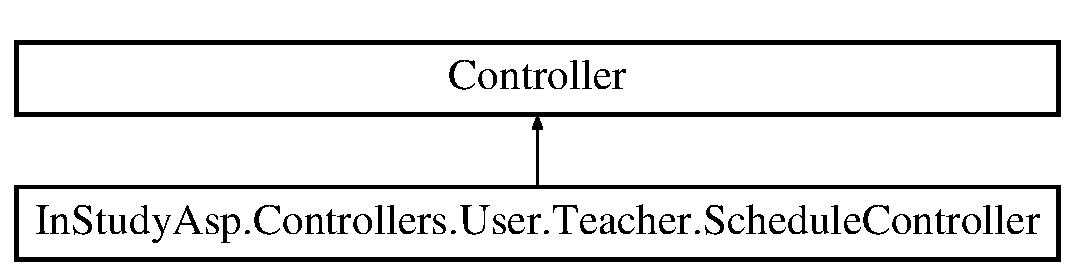
\includegraphics[height=2.000000cm]{class_in_study_asp_1_1_controllers_1_1_user_1_1_teacher_1_1_schedule_controller}
\end{center}
\end{figure}
\subsection*{Public Member Functions}
\begin{DoxyCompactItemize}
\item 
\hyperlink{class_in_study_asp_1_1_controllers_1_1_user_1_1_teacher_1_1_schedule_controller_aa5f4315593095a1c5065795fbf082a6c}{Schedule\+Controller} (\hyperlink{interface_repo_1_1_common_1_1_i_generic_repository}{I\+Generic\+Repository}$<$ \hyperlink{class_e_f_oracle_1_1_model_1_1_t_e_a_c_h_e_r}{T\+E\+A\+C\+H\+ER} $>$ \+\_\+teachers, \hyperlink{interface_repo_1_1_common_1_1_i_generic_repository}{I\+Generic\+Repository}$<$ \hyperlink{class_e_f_oracle_1_1_model_1_1_g_r_o_u_p}{G\+R\+O\+UP} $>$ \+\_\+groups, \hyperlink{class_repo_1_1_schedule_repository}{Schedule\+Repository} \+\_\+schedules, \hyperlink{interface_repo_1_1_common_1_1_i_generic_repository}{I\+Generic\+Repository}$<$ \hyperlink{class_e_f_oracle_1_1_model_1_1_d_i_s_c_i_p_l_i_n_e}{D\+I\+S\+C\+I\+P\+L\+I\+NE} $>$ \+\_\+disciplines)
\begin{DoxyCompactList}\small\item\em C\+T\+OR for Ninject, and get current \hyperlink{namespace_in_study_asp_1_1_controllers_1_1_user_1_1_teacher}{Teacher} from System.\+Web.\+Http\+Context. \end{DoxyCompactList}\item 
Action\+Result \hyperlink{class_in_study_asp_1_1_controllers_1_1_user_1_1_teacher_1_1_schedule_controller_a56b0d71c5c5639e0a9bd708a3535af6c}{Index} ()
\begin{DoxyCompactList}\small\item\em Task returns List of Schedules for current user(teacher) \end{DoxyCompactList}\item 
Action\+Result \hyperlink{class_in_study_asp_1_1_controllers_1_1_user_1_1_teacher_1_1_schedule_controller_aeaefe8512d47c31ed3afea285cae647d}{New} ()
\begin{DoxyCompactList}\small\item\em \begin{DoxyVerb}\end{DoxyVerb}
 \end{DoxyCompactList}\item 
Action\+Result \hyperlink{class_in_study_asp_1_1_controllers_1_1_user_1_1_teacher_1_1_schedule_controller_a8460ca79030e193cfb5367a0b51f6933}{Edit\+Post} (\hyperlink{class_in_study_asp_1_1_models_1_1_user_1_1_teacher_1_1_view_model_schedule}{View\+Model\+Schedule} \+\_\+schedule)
\begin{DoxyCompactList}\small\item\em Saving data from new or existing S\+C\+H\+E\+D\+U\+LE. \end{DoxyCompactList}\item 
Action\+Result \hyperlink{class_in_study_asp_1_1_controllers_1_1_user_1_1_teacher_1_1_schedule_controller_a822c9455259b96a96ae333d25ca7bf1a}{Edit\+Get} ()
\begin{DoxyCompactList}\small\item\em Geting page to Edit S\+C\+H\+E\+D\+U\+LE There is using P\+O\+ST request to pass multiple params for multiple columns Primary Key. \end{DoxyCompactList}\item 
Action\+Result \hyperlink{class_in_study_asp_1_1_controllers_1_1_user_1_1_teacher_1_1_schedule_controller_ad44fb1d37e6119aece41d3b71cb81ec8}{Delete} ()
\begin{DoxyCompactList}\small\item\em Action to delete S\+C\+H\+E\+D\+U\+LE. \end{DoxyCompactList}\end{DoxyCompactItemize}
\subsection*{Private Attributes}
\begin{DoxyCompactItemize}
\item 
\hyperlink{interface_repo_1_1_common_1_1_i_generic_repository}{I\+Generic\+Repository}$<$ \hyperlink{class_e_f_oracle_1_1_model_1_1_t_e_a_c_h_e_r}{T\+E\+A\+C\+H\+ER} $>$ \hyperlink{class_in_study_asp_1_1_controllers_1_1_user_1_1_teacher_1_1_schedule_controller_a74c7bae1cf29eef4b2c4b10b919f7f3f}{teachers}
\item 
\hyperlink{interface_repo_1_1_common_1_1_i_generic_repository}{I\+Generic\+Repository}$<$ \hyperlink{class_e_f_oracle_1_1_model_1_1_g_r_o_u_p}{G\+R\+O\+UP} $>$ \hyperlink{class_in_study_asp_1_1_controllers_1_1_user_1_1_teacher_1_1_schedule_controller_adca9d4990e412a7a5723c95b682fcba2}{groups}
\item 
\hyperlink{interface_repo_1_1_common_1_1_i_generic_repository}{I\+Generic\+Repository}$<$ \hyperlink{class_e_f_oracle_1_1_model_1_1_s_c_h_e_d_u_l_e}{S\+C\+H\+E\+D\+U\+LE} $>$ \hyperlink{class_in_study_asp_1_1_controllers_1_1_user_1_1_teacher_1_1_schedule_controller_aed008ef3307f7b8acecf751b084f9aad}{schedules}
\item 
\hyperlink{interface_repo_1_1_common_1_1_i_generic_repository}{I\+Generic\+Repository}$<$ \hyperlink{class_e_f_oracle_1_1_model_1_1_d_i_s_c_i_p_l_i_n_e}{D\+I\+S\+C\+I\+P\+L\+I\+NE} $>$ \hyperlink{class_in_study_asp_1_1_controllers_1_1_user_1_1_teacher_1_1_schedule_controller_a4102c2015fbace8b8213c9e3da2f72a8}{disciplines}
\item 
\hyperlink{class_e_f_oracle_1_1_model_1_1_t_e_a_c_h_e_r}{T\+E\+A\+C\+H\+ER} \hyperlink{class_in_study_asp_1_1_controllers_1_1_user_1_1_teacher_1_1_schedule_controller_a38f4c4a18010275b1be2ac2b87e5fc9b}{teacher}
\end{DoxyCompactItemize}


\subsection{Detailed Description}
contains C\+R\+UD actions for S\+C\+H\+E\+D\+U\+L\+ES 

\subsection{Constructor \& Destructor Documentation}
\mbox{\Hypertarget{class_in_study_asp_1_1_controllers_1_1_user_1_1_teacher_1_1_schedule_controller_aa5f4315593095a1c5065795fbf082a6c}\label{class_in_study_asp_1_1_controllers_1_1_user_1_1_teacher_1_1_schedule_controller_aa5f4315593095a1c5065795fbf082a6c}} 
\index{In\+Study\+Asp\+::\+Controllers\+::\+User\+::\+Teacher\+::\+Schedule\+Controller@{In\+Study\+Asp\+::\+Controllers\+::\+User\+::\+Teacher\+::\+Schedule\+Controller}!Schedule\+Controller@{Schedule\+Controller}}
\index{Schedule\+Controller@{Schedule\+Controller}!In\+Study\+Asp\+::\+Controllers\+::\+User\+::\+Teacher\+::\+Schedule\+Controller@{In\+Study\+Asp\+::\+Controllers\+::\+User\+::\+Teacher\+::\+Schedule\+Controller}}
\subsubsection{\texorpdfstring{Schedule\+Controller()}{ScheduleController()}}
{\footnotesize\ttfamily In\+Study\+Asp.\+Controllers.\+User.\+Teacher.\+Schedule\+Controller.\+Schedule\+Controller (\begin{DoxyParamCaption}\item[{\hyperlink{interface_repo_1_1_common_1_1_i_generic_repository}{I\+Generic\+Repository}$<$ \hyperlink{class_e_f_oracle_1_1_model_1_1_t_e_a_c_h_e_r}{T\+E\+A\+C\+H\+ER} $>$}]{\+\_\+teachers,  }\item[{\hyperlink{interface_repo_1_1_common_1_1_i_generic_repository}{I\+Generic\+Repository}$<$ \hyperlink{class_e_f_oracle_1_1_model_1_1_g_r_o_u_p}{G\+R\+O\+UP} $>$}]{\+\_\+groups,  }\item[{\hyperlink{class_repo_1_1_schedule_repository}{Schedule\+Repository}}]{\+\_\+schedules,  }\item[{\hyperlink{interface_repo_1_1_common_1_1_i_generic_repository}{I\+Generic\+Repository}$<$ \hyperlink{class_e_f_oracle_1_1_model_1_1_d_i_s_c_i_p_l_i_n_e}{D\+I\+S\+C\+I\+P\+L\+I\+NE} $>$}]{\+\_\+disciplines }\end{DoxyParamCaption})}



C\+T\+OR for Ninject, and get current \hyperlink{namespace_in_study_asp_1_1_controllers_1_1_user_1_1_teacher}{Teacher} from System.\+Web.\+Http\+Context. 



\subsection{Member Function Documentation}
\mbox{\Hypertarget{class_in_study_asp_1_1_controllers_1_1_user_1_1_teacher_1_1_schedule_controller_ad44fb1d37e6119aece41d3b71cb81ec8}\label{class_in_study_asp_1_1_controllers_1_1_user_1_1_teacher_1_1_schedule_controller_ad44fb1d37e6119aece41d3b71cb81ec8}} 
\index{In\+Study\+Asp\+::\+Controllers\+::\+User\+::\+Teacher\+::\+Schedule\+Controller@{In\+Study\+Asp\+::\+Controllers\+::\+User\+::\+Teacher\+::\+Schedule\+Controller}!Delete@{Delete}}
\index{Delete@{Delete}!In\+Study\+Asp\+::\+Controllers\+::\+User\+::\+Teacher\+::\+Schedule\+Controller@{In\+Study\+Asp\+::\+Controllers\+::\+User\+::\+Teacher\+::\+Schedule\+Controller}}
\subsubsection{\texorpdfstring{Delete()}{Delete()}}
{\footnotesize\ttfamily Action\+Result In\+Study\+Asp.\+Controllers.\+User.\+Teacher.\+Schedule\+Controller.\+Delete (\begin{DoxyParamCaption}{ }\end{DoxyParamCaption})}



Action to delete S\+C\+H\+E\+D\+U\+LE. 

\mbox{\Hypertarget{class_in_study_asp_1_1_controllers_1_1_user_1_1_teacher_1_1_schedule_controller_a822c9455259b96a96ae333d25ca7bf1a}\label{class_in_study_asp_1_1_controllers_1_1_user_1_1_teacher_1_1_schedule_controller_a822c9455259b96a96ae333d25ca7bf1a}} 
\index{In\+Study\+Asp\+::\+Controllers\+::\+User\+::\+Teacher\+::\+Schedule\+Controller@{In\+Study\+Asp\+::\+Controllers\+::\+User\+::\+Teacher\+::\+Schedule\+Controller}!Edit\+Get@{Edit\+Get}}
\index{Edit\+Get@{Edit\+Get}!In\+Study\+Asp\+::\+Controllers\+::\+User\+::\+Teacher\+::\+Schedule\+Controller@{In\+Study\+Asp\+::\+Controllers\+::\+User\+::\+Teacher\+::\+Schedule\+Controller}}
\subsubsection{\texorpdfstring{Edit\+Get()}{EditGet()}}
{\footnotesize\ttfamily Action\+Result In\+Study\+Asp.\+Controllers.\+User.\+Teacher.\+Schedule\+Controller.\+Edit\+Get (\begin{DoxyParamCaption}{ }\end{DoxyParamCaption})}



Geting page to Edit S\+C\+H\+E\+D\+U\+LE There is using P\+O\+ST request to pass multiple params for multiple columns Primary Key. 

\mbox{\Hypertarget{class_in_study_asp_1_1_controllers_1_1_user_1_1_teacher_1_1_schedule_controller_a8460ca79030e193cfb5367a0b51f6933}\label{class_in_study_asp_1_1_controllers_1_1_user_1_1_teacher_1_1_schedule_controller_a8460ca79030e193cfb5367a0b51f6933}} 
\index{In\+Study\+Asp\+::\+Controllers\+::\+User\+::\+Teacher\+::\+Schedule\+Controller@{In\+Study\+Asp\+::\+Controllers\+::\+User\+::\+Teacher\+::\+Schedule\+Controller}!Edit\+Post@{Edit\+Post}}
\index{Edit\+Post@{Edit\+Post}!In\+Study\+Asp\+::\+Controllers\+::\+User\+::\+Teacher\+::\+Schedule\+Controller@{In\+Study\+Asp\+::\+Controllers\+::\+User\+::\+Teacher\+::\+Schedule\+Controller}}
\subsubsection{\texorpdfstring{Edit\+Post()}{EditPost()}}
{\footnotesize\ttfamily Action\+Result In\+Study\+Asp.\+Controllers.\+User.\+Teacher.\+Schedule\+Controller.\+Edit\+Post (\begin{DoxyParamCaption}\item[{\hyperlink{class_in_study_asp_1_1_models_1_1_user_1_1_teacher_1_1_view_model_schedule}{View\+Model\+Schedule}}]{\+\_\+schedule }\end{DoxyParamCaption})}



Saving data from new or existing S\+C\+H\+E\+D\+U\+LE. 

\mbox{\Hypertarget{class_in_study_asp_1_1_controllers_1_1_user_1_1_teacher_1_1_schedule_controller_a56b0d71c5c5639e0a9bd708a3535af6c}\label{class_in_study_asp_1_1_controllers_1_1_user_1_1_teacher_1_1_schedule_controller_a56b0d71c5c5639e0a9bd708a3535af6c}} 
\index{In\+Study\+Asp\+::\+Controllers\+::\+User\+::\+Teacher\+::\+Schedule\+Controller@{In\+Study\+Asp\+::\+Controllers\+::\+User\+::\+Teacher\+::\+Schedule\+Controller}!Index@{Index}}
\index{Index@{Index}!In\+Study\+Asp\+::\+Controllers\+::\+User\+::\+Teacher\+::\+Schedule\+Controller@{In\+Study\+Asp\+::\+Controllers\+::\+User\+::\+Teacher\+::\+Schedule\+Controller}}
\subsubsection{\texorpdfstring{Index()}{Index()}}
{\footnotesize\ttfamily Action\+Result In\+Study\+Asp.\+Controllers.\+User.\+Teacher.\+Schedule\+Controller.\+Index (\begin{DoxyParamCaption}{ }\end{DoxyParamCaption})}



Task returns List of Schedules for current user(teacher) 

\mbox{\Hypertarget{class_in_study_asp_1_1_controllers_1_1_user_1_1_teacher_1_1_schedule_controller_aeaefe8512d47c31ed3afea285cae647d}\label{class_in_study_asp_1_1_controllers_1_1_user_1_1_teacher_1_1_schedule_controller_aeaefe8512d47c31ed3afea285cae647d}} 
\index{In\+Study\+Asp\+::\+Controllers\+::\+User\+::\+Teacher\+::\+Schedule\+Controller@{In\+Study\+Asp\+::\+Controllers\+::\+User\+::\+Teacher\+::\+Schedule\+Controller}!New@{New}}
\index{New@{New}!In\+Study\+Asp\+::\+Controllers\+::\+User\+::\+Teacher\+::\+Schedule\+Controller@{In\+Study\+Asp\+::\+Controllers\+::\+User\+::\+Teacher\+::\+Schedule\+Controller}}
\subsubsection{\texorpdfstring{New()}{New()}}
{\footnotesize\ttfamily Action\+Result In\+Study\+Asp.\+Controllers.\+User.\+Teacher.\+Schedule\+Controller.\+New (\begin{DoxyParamCaption}{ }\end{DoxyParamCaption})}



\begin{DoxyVerb}\end{DoxyVerb}
 



\subsection{Member Data Documentation}
\mbox{\Hypertarget{class_in_study_asp_1_1_controllers_1_1_user_1_1_teacher_1_1_schedule_controller_a4102c2015fbace8b8213c9e3da2f72a8}\label{class_in_study_asp_1_1_controllers_1_1_user_1_1_teacher_1_1_schedule_controller_a4102c2015fbace8b8213c9e3da2f72a8}} 
\index{In\+Study\+Asp\+::\+Controllers\+::\+User\+::\+Teacher\+::\+Schedule\+Controller@{In\+Study\+Asp\+::\+Controllers\+::\+User\+::\+Teacher\+::\+Schedule\+Controller}!disciplines@{disciplines}}
\index{disciplines@{disciplines}!In\+Study\+Asp\+::\+Controllers\+::\+User\+::\+Teacher\+::\+Schedule\+Controller@{In\+Study\+Asp\+::\+Controllers\+::\+User\+::\+Teacher\+::\+Schedule\+Controller}}
\subsubsection{\texorpdfstring{disciplines}{disciplines}}
{\footnotesize\ttfamily \hyperlink{interface_repo_1_1_common_1_1_i_generic_repository}{I\+Generic\+Repository}$<$\hyperlink{class_e_f_oracle_1_1_model_1_1_d_i_s_c_i_p_l_i_n_e}{D\+I\+S\+C\+I\+P\+L\+I\+NE}$>$ In\+Study\+Asp.\+Controllers.\+User.\+Teacher.\+Schedule\+Controller.\+disciplines\hspace{0.3cm}{\ttfamily [private]}}

\mbox{\Hypertarget{class_in_study_asp_1_1_controllers_1_1_user_1_1_teacher_1_1_schedule_controller_adca9d4990e412a7a5723c95b682fcba2}\label{class_in_study_asp_1_1_controllers_1_1_user_1_1_teacher_1_1_schedule_controller_adca9d4990e412a7a5723c95b682fcba2}} 
\index{In\+Study\+Asp\+::\+Controllers\+::\+User\+::\+Teacher\+::\+Schedule\+Controller@{In\+Study\+Asp\+::\+Controllers\+::\+User\+::\+Teacher\+::\+Schedule\+Controller}!groups@{groups}}
\index{groups@{groups}!In\+Study\+Asp\+::\+Controllers\+::\+User\+::\+Teacher\+::\+Schedule\+Controller@{In\+Study\+Asp\+::\+Controllers\+::\+User\+::\+Teacher\+::\+Schedule\+Controller}}
\subsubsection{\texorpdfstring{groups}{groups}}
{\footnotesize\ttfamily \hyperlink{interface_repo_1_1_common_1_1_i_generic_repository}{I\+Generic\+Repository}$<$\hyperlink{class_e_f_oracle_1_1_model_1_1_g_r_o_u_p}{G\+R\+O\+UP}$>$ In\+Study\+Asp.\+Controllers.\+User.\+Teacher.\+Schedule\+Controller.\+groups\hspace{0.3cm}{\ttfamily [private]}}

\mbox{\Hypertarget{class_in_study_asp_1_1_controllers_1_1_user_1_1_teacher_1_1_schedule_controller_aed008ef3307f7b8acecf751b084f9aad}\label{class_in_study_asp_1_1_controllers_1_1_user_1_1_teacher_1_1_schedule_controller_aed008ef3307f7b8acecf751b084f9aad}} 
\index{In\+Study\+Asp\+::\+Controllers\+::\+User\+::\+Teacher\+::\+Schedule\+Controller@{In\+Study\+Asp\+::\+Controllers\+::\+User\+::\+Teacher\+::\+Schedule\+Controller}!schedules@{schedules}}
\index{schedules@{schedules}!In\+Study\+Asp\+::\+Controllers\+::\+User\+::\+Teacher\+::\+Schedule\+Controller@{In\+Study\+Asp\+::\+Controllers\+::\+User\+::\+Teacher\+::\+Schedule\+Controller}}
\subsubsection{\texorpdfstring{schedules}{schedules}}
{\footnotesize\ttfamily \hyperlink{interface_repo_1_1_common_1_1_i_generic_repository}{I\+Generic\+Repository}$<$\hyperlink{class_e_f_oracle_1_1_model_1_1_s_c_h_e_d_u_l_e}{S\+C\+H\+E\+D\+U\+LE}$>$ In\+Study\+Asp.\+Controllers.\+User.\+Teacher.\+Schedule\+Controller.\+schedules\hspace{0.3cm}{\ttfamily [private]}}

\mbox{\Hypertarget{class_in_study_asp_1_1_controllers_1_1_user_1_1_teacher_1_1_schedule_controller_a38f4c4a18010275b1be2ac2b87e5fc9b}\label{class_in_study_asp_1_1_controllers_1_1_user_1_1_teacher_1_1_schedule_controller_a38f4c4a18010275b1be2ac2b87e5fc9b}} 
\index{In\+Study\+Asp\+::\+Controllers\+::\+User\+::\+Teacher\+::\+Schedule\+Controller@{In\+Study\+Asp\+::\+Controllers\+::\+User\+::\+Teacher\+::\+Schedule\+Controller}!teacher@{teacher}}
\index{teacher@{teacher}!In\+Study\+Asp\+::\+Controllers\+::\+User\+::\+Teacher\+::\+Schedule\+Controller@{In\+Study\+Asp\+::\+Controllers\+::\+User\+::\+Teacher\+::\+Schedule\+Controller}}
\subsubsection{\texorpdfstring{teacher}{teacher}}
{\footnotesize\ttfamily \hyperlink{class_e_f_oracle_1_1_model_1_1_t_e_a_c_h_e_r}{T\+E\+A\+C\+H\+ER} In\+Study\+Asp.\+Controllers.\+User.\+Teacher.\+Schedule\+Controller.\+teacher\hspace{0.3cm}{\ttfamily [private]}}

\mbox{\Hypertarget{class_in_study_asp_1_1_controllers_1_1_user_1_1_teacher_1_1_schedule_controller_a74c7bae1cf29eef4b2c4b10b919f7f3f}\label{class_in_study_asp_1_1_controllers_1_1_user_1_1_teacher_1_1_schedule_controller_a74c7bae1cf29eef4b2c4b10b919f7f3f}} 
\index{In\+Study\+Asp\+::\+Controllers\+::\+User\+::\+Teacher\+::\+Schedule\+Controller@{In\+Study\+Asp\+::\+Controllers\+::\+User\+::\+Teacher\+::\+Schedule\+Controller}!teachers@{teachers}}
\index{teachers@{teachers}!In\+Study\+Asp\+::\+Controllers\+::\+User\+::\+Teacher\+::\+Schedule\+Controller@{In\+Study\+Asp\+::\+Controllers\+::\+User\+::\+Teacher\+::\+Schedule\+Controller}}
\subsubsection{\texorpdfstring{teachers}{teachers}}
{\footnotesize\ttfamily \hyperlink{interface_repo_1_1_common_1_1_i_generic_repository}{I\+Generic\+Repository}$<$\hyperlink{class_e_f_oracle_1_1_model_1_1_t_e_a_c_h_e_r}{T\+E\+A\+C\+H\+ER}$>$ In\+Study\+Asp.\+Controllers.\+User.\+Teacher.\+Schedule\+Controller.\+teachers\hspace{0.3cm}{\ttfamily [private]}}



The documentation for this class was generated from the following file\+:\begin{DoxyCompactItemize}
\item 
D\+:/\+\_\+\+W\+O\+R\+K/\+\_\+\+S\+T\+E\+P/\+In\+Study\+Asp/\+In\+Study\+Asp/\+Controllers/\+User/\+Teacher/\hyperlink{_schedule_controller_8cs}{Schedule\+Controller.\+cs}\end{DoxyCompactItemize}

\hypertarget{class_e_f_oracle_1_1_model_1_1_schedule_metadata}{}\section{E\+F\+Oracle.\+Model.\+Schedule\+Metadata Class Reference}
\label{class_e_f_oracle_1_1_model_1_1_schedule_metadata}\index{E\+F\+Oracle.\+Model.\+Schedule\+Metadata@{E\+F\+Oracle.\+Model.\+Schedule\+Metadata}}
\subsection*{Properties}
\begin{DoxyCompactItemize}
\item 
decimal \hyperlink{class_e_f_oracle_1_1_model_1_1_schedule_metadata_a34f92b2df8eef5012a62b2fc88384f8e}{T\+E\+A\+C\+H\+E\+R\+\_\+\+ID}\hspace{0.3cm}{\ttfamily  \mbox{[}get, set\mbox{]}}
\item 
string \hyperlink{class_e_f_oracle_1_1_model_1_1_schedule_metadata_aaafcba28fc98d8b0e1f7c1d01fa162f7}{G\+R\+O\+U\+P\+\_\+\+C\+O\+DE}\hspace{0.3cm}{\ttfamily  \mbox{[}get, set\mbox{]}}
\item 
decimal \hyperlink{class_e_f_oracle_1_1_model_1_1_schedule_metadata_a3f7670dba054bc7de4fb175882dfdaa7}{D\+I\+S\+C\+I\+P\+L\+I\+N\+E\+\_\+\+C\+O\+DE}\hspace{0.3cm}{\ttfamily  \mbox{[}get, set\mbox{]}}
\item 
Date\+Time \hyperlink{class_e_f_oracle_1_1_model_1_1_schedule_metadata_a395ee9fa9ce0ee5e2266c3595d232013}{S\+C\+H\+E\+D\+U\+L\+E\+\_\+\+D\+A\+TE}\hspace{0.3cm}{\ttfamily  \mbox{[}get, set\mbox{]}}
\item 
decimal \hyperlink{class_e_f_oracle_1_1_model_1_1_schedule_metadata_a2328ac1c9c8acf363774625016cc2f78}{S\+C\+H\+E\+D\+U\+L\+E\+\_\+\+R\+O\+OM}\hspace{0.3cm}{\ttfamily  \mbox{[}get, set\mbox{]}}
\item 
virtual \hyperlink{class_e_f_oracle_1_1_model_1_1_d_i_s_c_i_p_l_i_n_e}{D\+I\+S\+C\+I\+P\+L\+I\+NE} \hyperlink{class_e_f_oracle_1_1_model_1_1_schedule_metadata_a1b0e8d574ca3bba4f029cdee8c4d12cb}{D\+I\+S\+C\+I\+P\+L\+I\+NE}\hspace{0.3cm}{\ttfamily  \mbox{[}get, set\mbox{]}}
\item 
virtual \hyperlink{class_e_f_oracle_1_1_model_1_1_g_r_o_u_p}{G\+R\+O\+UP} \hyperlink{class_e_f_oracle_1_1_model_1_1_schedule_metadata_ad1249eb1718f7573d421991f6c747219}{G\+R\+O\+UP}\hspace{0.3cm}{\ttfamily  \mbox{[}get, set\mbox{]}}
\item 
virtual \hyperlink{class_e_f_oracle_1_1_model_1_1_t_e_a_c_h_e_r}{T\+E\+A\+C\+H\+ER} \hyperlink{class_e_f_oracle_1_1_model_1_1_schedule_metadata_af6379f2c8f84516657cd2f7155b954b4}{T\+E\+A\+C\+H\+ER}\hspace{0.3cm}{\ttfamily  \mbox{[}get, set\mbox{]}}
\end{DoxyCompactItemize}


\subsection{Property Documentation}
\mbox{\Hypertarget{class_e_f_oracle_1_1_model_1_1_schedule_metadata_a1b0e8d574ca3bba4f029cdee8c4d12cb}\label{class_e_f_oracle_1_1_model_1_1_schedule_metadata_a1b0e8d574ca3bba4f029cdee8c4d12cb}} 
\index{E\+F\+Oracle\+::\+Model\+::\+Schedule\+Metadata@{E\+F\+Oracle\+::\+Model\+::\+Schedule\+Metadata}!D\+I\+S\+C\+I\+P\+L\+I\+NE@{D\+I\+S\+C\+I\+P\+L\+I\+NE}}
\index{D\+I\+S\+C\+I\+P\+L\+I\+NE@{D\+I\+S\+C\+I\+P\+L\+I\+NE}!E\+F\+Oracle\+::\+Model\+::\+Schedule\+Metadata@{E\+F\+Oracle\+::\+Model\+::\+Schedule\+Metadata}}
\subsubsection{\texorpdfstring{D\+I\+S\+C\+I\+P\+L\+I\+NE}{DISCIPLINE}}
{\footnotesize\ttfamily virtual \hyperlink{class_e_f_oracle_1_1_model_1_1_d_i_s_c_i_p_l_i_n_e}{D\+I\+S\+C\+I\+P\+L\+I\+NE} E\+F\+Oracle.\+Model.\+Schedule\+Metadata.\+D\+I\+S\+C\+I\+P\+L\+I\+NE\hspace{0.3cm}{\ttfamily [get]}, {\ttfamily [set]}}

\mbox{\Hypertarget{class_e_f_oracle_1_1_model_1_1_schedule_metadata_a3f7670dba054bc7de4fb175882dfdaa7}\label{class_e_f_oracle_1_1_model_1_1_schedule_metadata_a3f7670dba054bc7de4fb175882dfdaa7}} 
\index{E\+F\+Oracle\+::\+Model\+::\+Schedule\+Metadata@{E\+F\+Oracle\+::\+Model\+::\+Schedule\+Metadata}!D\+I\+S\+C\+I\+P\+L\+I\+N\+E\+\_\+\+C\+O\+DE@{D\+I\+S\+C\+I\+P\+L\+I\+N\+E\+\_\+\+C\+O\+DE}}
\index{D\+I\+S\+C\+I\+P\+L\+I\+N\+E\+\_\+\+C\+O\+DE@{D\+I\+S\+C\+I\+P\+L\+I\+N\+E\+\_\+\+C\+O\+DE}!E\+F\+Oracle\+::\+Model\+::\+Schedule\+Metadata@{E\+F\+Oracle\+::\+Model\+::\+Schedule\+Metadata}}
\subsubsection{\texorpdfstring{D\+I\+S\+C\+I\+P\+L\+I\+N\+E\+\_\+\+C\+O\+DE}{DISCIPLINE\_CODE}}
{\footnotesize\ttfamily decimal E\+F\+Oracle.\+Model.\+Schedule\+Metadata.\+D\+I\+S\+C\+I\+P\+L\+I\+N\+E\+\_\+\+C\+O\+DE\hspace{0.3cm}{\ttfamily [get]}, {\ttfamily [set]}}

\mbox{\Hypertarget{class_e_f_oracle_1_1_model_1_1_schedule_metadata_ad1249eb1718f7573d421991f6c747219}\label{class_e_f_oracle_1_1_model_1_1_schedule_metadata_ad1249eb1718f7573d421991f6c747219}} 
\index{E\+F\+Oracle\+::\+Model\+::\+Schedule\+Metadata@{E\+F\+Oracle\+::\+Model\+::\+Schedule\+Metadata}!G\+R\+O\+UP@{G\+R\+O\+UP}}
\index{G\+R\+O\+UP@{G\+R\+O\+UP}!E\+F\+Oracle\+::\+Model\+::\+Schedule\+Metadata@{E\+F\+Oracle\+::\+Model\+::\+Schedule\+Metadata}}
\subsubsection{\texorpdfstring{G\+R\+O\+UP}{GROUP}}
{\footnotesize\ttfamily virtual \hyperlink{class_e_f_oracle_1_1_model_1_1_g_r_o_u_p}{G\+R\+O\+UP} E\+F\+Oracle.\+Model.\+Schedule\+Metadata.\+G\+R\+O\+UP\hspace{0.3cm}{\ttfamily [get]}, {\ttfamily [set]}}

\mbox{\Hypertarget{class_e_f_oracle_1_1_model_1_1_schedule_metadata_aaafcba28fc98d8b0e1f7c1d01fa162f7}\label{class_e_f_oracle_1_1_model_1_1_schedule_metadata_aaafcba28fc98d8b0e1f7c1d01fa162f7}} 
\index{E\+F\+Oracle\+::\+Model\+::\+Schedule\+Metadata@{E\+F\+Oracle\+::\+Model\+::\+Schedule\+Metadata}!G\+R\+O\+U\+P\+\_\+\+C\+O\+DE@{G\+R\+O\+U\+P\+\_\+\+C\+O\+DE}}
\index{G\+R\+O\+U\+P\+\_\+\+C\+O\+DE@{G\+R\+O\+U\+P\+\_\+\+C\+O\+DE}!E\+F\+Oracle\+::\+Model\+::\+Schedule\+Metadata@{E\+F\+Oracle\+::\+Model\+::\+Schedule\+Metadata}}
\subsubsection{\texorpdfstring{G\+R\+O\+U\+P\+\_\+\+C\+O\+DE}{GROUP\_CODE}}
{\footnotesize\ttfamily string E\+F\+Oracle.\+Model.\+Schedule\+Metadata.\+G\+R\+O\+U\+P\+\_\+\+C\+O\+DE\hspace{0.3cm}{\ttfamily [get]}, {\ttfamily [set]}}

\mbox{\Hypertarget{class_e_f_oracle_1_1_model_1_1_schedule_metadata_a395ee9fa9ce0ee5e2266c3595d232013}\label{class_e_f_oracle_1_1_model_1_1_schedule_metadata_a395ee9fa9ce0ee5e2266c3595d232013}} 
\index{E\+F\+Oracle\+::\+Model\+::\+Schedule\+Metadata@{E\+F\+Oracle\+::\+Model\+::\+Schedule\+Metadata}!S\+C\+H\+E\+D\+U\+L\+E\+\_\+\+D\+A\+TE@{S\+C\+H\+E\+D\+U\+L\+E\+\_\+\+D\+A\+TE}}
\index{S\+C\+H\+E\+D\+U\+L\+E\+\_\+\+D\+A\+TE@{S\+C\+H\+E\+D\+U\+L\+E\+\_\+\+D\+A\+TE}!E\+F\+Oracle\+::\+Model\+::\+Schedule\+Metadata@{E\+F\+Oracle\+::\+Model\+::\+Schedule\+Metadata}}
\subsubsection{\texorpdfstring{S\+C\+H\+E\+D\+U\+L\+E\+\_\+\+D\+A\+TE}{SCHEDULE\_DATE}}
{\footnotesize\ttfamily Date\+Time E\+F\+Oracle.\+Model.\+Schedule\+Metadata.\+S\+C\+H\+E\+D\+U\+L\+E\+\_\+\+D\+A\+TE\hspace{0.3cm}{\ttfamily [get]}, {\ttfamily [set]}}

\mbox{\Hypertarget{class_e_f_oracle_1_1_model_1_1_schedule_metadata_a2328ac1c9c8acf363774625016cc2f78}\label{class_e_f_oracle_1_1_model_1_1_schedule_metadata_a2328ac1c9c8acf363774625016cc2f78}} 
\index{E\+F\+Oracle\+::\+Model\+::\+Schedule\+Metadata@{E\+F\+Oracle\+::\+Model\+::\+Schedule\+Metadata}!S\+C\+H\+E\+D\+U\+L\+E\+\_\+\+R\+O\+OM@{S\+C\+H\+E\+D\+U\+L\+E\+\_\+\+R\+O\+OM}}
\index{S\+C\+H\+E\+D\+U\+L\+E\+\_\+\+R\+O\+OM@{S\+C\+H\+E\+D\+U\+L\+E\+\_\+\+R\+O\+OM}!E\+F\+Oracle\+::\+Model\+::\+Schedule\+Metadata@{E\+F\+Oracle\+::\+Model\+::\+Schedule\+Metadata}}
\subsubsection{\texorpdfstring{S\+C\+H\+E\+D\+U\+L\+E\+\_\+\+R\+O\+OM}{SCHEDULE\_ROOM}}
{\footnotesize\ttfamily decimal E\+F\+Oracle.\+Model.\+Schedule\+Metadata.\+S\+C\+H\+E\+D\+U\+L\+E\+\_\+\+R\+O\+OM\hspace{0.3cm}{\ttfamily [get]}, {\ttfamily [set]}}

\mbox{\Hypertarget{class_e_f_oracle_1_1_model_1_1_schedule_metadata_af6379f2c8f84516657cd2f7155b954b4}\label{class_e_f_oracle_1_1_model_1_1_schedule_metadata_af6379f2c8f84516657cd2f7155b954b4}} 
\index{E\+F\+Oracle\+::\+Model\+::\+Schedule\+Metadata@{E\+F\+Oracle\+::\+Model\+::\+Schedule\+Metadata}!T\+E\+A\+C\+H\+ER@{T\+E\+A\+C\+H\+ER}}
\index{T\+E\+A\+C\+H\+ER@{T\+E\+A\+C\+H\+ER}!E\+F\+Oracle\+::\+Model\+::\+Schedule\+Metadata@{E\+F\+Oracle\+::\+Model\+::\+Schedule\+Metadata}}
\subsubsection{\texorpdfstring{T\+E\+A\+C\+H\+ER}{TEACHER}}
{\footnotesize\ttfamily virtual \hyperlink{class_e_f_oracle_1_1_model_1_1_t_e_a_c_h_e_r}{T\+E\+A\+C\+H\+ER} E\+F\+Oracle.\+Model.\+Schedule\+Metadata.\+T\+E\+A\+C\+H\+ER\hspace{0.3cm}{\ttfamily [get]}, {\ttfamily [set]}}

\mbox{\Hypertarget{class_e_f_oracle_1_1_model_1_1_schedule_metadata_a34f92b2df8eef5012a62b2fc88384f8e}\label{class_e_f_oracle_1_1_model_1_1_schedule_metadata_a34f92b2df8eef5012a62b2fc88384f8e}} 
\index{E\+F\+Oracle\+::\+Model\+::\+Schedule\+Metadata@{E\+F\+Oracle\+::\+Model\+::\+Schedule\+Metadata}!T\+E\+A\+C\+H\+E\+R\+\_\+\+ID@{T\+E\+A\+C\+H\+E\+R\+\_\+\+ID}}
\index{T\+E\+A\+C\+H\+E\+R\+\_\+\+ID@{T\+E\+A\+C\+H\+E\+R\+\_\+\+ID}!E\+F\+Oracle\+::\+Model\+::\+Schedule\+Metadata@{E\+F\+Oracle\+::\+Model\+::\+Schedule\+Metadata}}
\subsubsection{\texorpdfstring{T\+E\+A\+C\+H\+E\+R\+\_\+\+ID}{TEACHER\_ID}}
{\footnotesize\ttfamily decimal E\+F\+Oracle.\+Model.\+Schedule\+Metadata.\+T\+E\+A\+C\+H\+E\+R\+\_\+\+ID\hspace{0.3cm}{\ttfamily [get]}, {\ttfamily [set]}}



The documentation for this class was generated from the following file\+:\begin{DoxyCompactItemize}
\item 
D\+:/\+\_\+\+W\+O\+R\+K/\+\_\+\+S\+T\+E\+P/\+In\+Study\+Asp/\+E\+F\+Oracle/\+Model/\+Extended/\hyperlink{_extended_2_s_c_h_e_d_u_l_e_8cs}{S\+C\+H\+E\+D\+U\+L\+E.\+cs}\end{DoxyCompactItemize}

\hypertarget{class_repo_1_1_schedule_repository}{}\section{Repo.\+Schedule\+Repository Class Reference}
\label{class_repo_1_1_schedule_repository}\index{Repo.\+Schedule\+Repository@{Repo.\+Schedule\+Repository}}
Inheritance diagram for Repo.\+Schedule\+Repository\+:\begin{figure}[H]
\begin{center}
\leavevmode
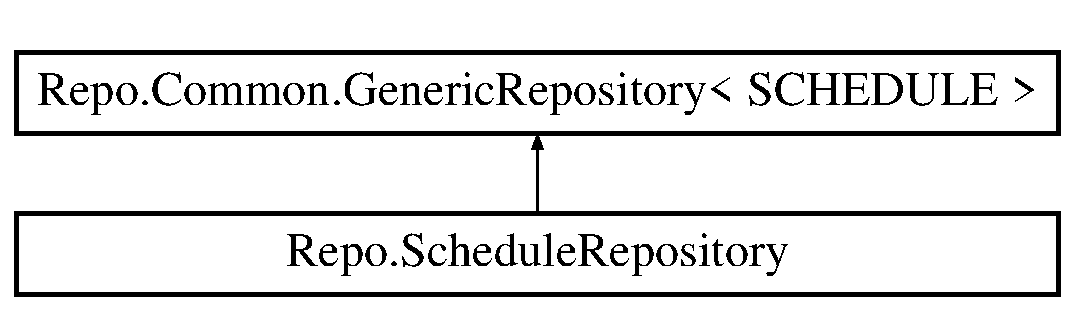
\includegraphics[height=2.000000cm]{class_repo_1_1_schedule_repository}
\end{center}
\end{figure}
\subsection*{Public Member Functions}
\begin{DoxyCompactItemize}
\item 
\hyperlink{class_repo_1_1_schedule_repository_ab99694ab2c74fa3af8d40b1e2783f187}{Schedule\+Repository} (Db\+Context context)
\end{DoxyCompactItemize}
\subsection*{Additional Inherited Members}


\subsection{Constructor \& Destructor Documentation}
\mbox{\Hypertarget{class_repo_1_1_schedule_repository_ab99694ab2c74fa3af8d40b1e2783f187}\label{class_repo_1_1_schedule_repository_ab99694ab2c74fa3af8d40b1e2783f187}} 
\index{Repo\+::\+Schedule\+Repository@{Repo\+::\+Schedule\+Repository}!Schedule\+Repository@{Schedule\+Repository}}
\index{Schedule\+Repository@{Schedule\+Repository}!Repo\+::\+Schedule\+Repository@{Repo\+::\+Schedule\+Repository}}
\subsubsection{\texorpdfstring{Schedule\+Repository()}{ScheduleRepository()}}
{\footnotesize\ttfamily Repo.\+Schedule\+Repository.\+Schedule\+Repository (\begin{DoxyParamCaption}\item[{Db\+Context}]{context }\end{DoxyParamCaption})}



The documentation for this class was generated from the following file\+:\begin{DoxyCompactItemize}
\item 
D\+:/\+\_\+\+W\+O\+R\+K/\+\_\+\+S\+T\+E\+P/\+In\+Study\+Asp/\+Repo/\hyperlink{_schedule_repository_8cs}{Schedule\+Repository.\+cs}\end{DoxyCompactItemize}

\hypertarget{class_e_f_oracle_1_1_model_1_1_s_t_u_d_e_n_t}{}\section{E\+F\+Oracle.\+Model.\+S\+T\+U\+D\+E\+NT Class Reference}
\label{class_e_f_oracle_1_1_model_1_1_s_t_u_d_e_n_t}\index{E\+F\+Oracle.\+Model.\+S\+T\+U\+D\+E\+NT@{E\+F\+Oracle.\+Model.\+S\+T\+U\+D\+E\+NT}}
\subsection*{Public Member Functions}
\begin{DoxyCompactItemize}
\item 
\hyperlink{class_e_f_oracle_1_1_model_1_1_s_t_u_d_e_n_t_a42c5fe0bd0b1873d403c457339dc6387}{S\+T\+U\+D\+E\+NT} ()
\end{DoxyCompactItemize}
\subsection*{Properties}
\begin{DoxyCompactItemize}
\item 
decimal \hyperlink{class_e_f_oracle_1_1_model_1_1_s_t_u_d_e_n_t_ac52552fb2577883bf22d24acd6263928}{S\+T\+U\+D\+E\+N\+T\+\_\+\+ID}\hspace{0.3cm}{\ttfamily  \mbox{[}get, set\mbox{]}}
\item 
string \hyperlink{class_e_f_oracle_1_1_model_1_1_s_t_u_d_e_n_t_a03789daa6023e5873d86b9dde2c913a5}{G\+R\+O\+U\+P\+\_\+\+C\+O\+DE}\hspace{0.3cm}{\ttfamily  \mbox{[}get, set\mbox{]}}
\item 
Date\+Time \hyperlink{class_e_f_oracle_1_1_model_1_1_s_t_u_d_e_n_t_ac98090401dae17df06850dedd8d20acf}{S\+T\+U\+D\+E\+N\+T\+\_\+\+S\+T\+A\+RT}\hspace{0.3cm}{\ttfamily  \mbox{[}get, set\mbox{]}}
\item 
string \hyperlink{class_e_f_oracle_1_1_model_1_1_s_t_u_d_e_n_t_aade79c3e50cdf2b7756ab476b9cadea7}{U\+S\+E\+R\+\_\+\+P\+H\+O\+NE}\hspace{0.3cm}{\ttfamily  \mbox{[}get, set\mbox{]}}
\item 
Date\+Time \hyperlink{class_e_f_oracle_1_1_model_1_1_s_t_u_d_e_n_t_ab80cc4d1a69f1a6fcc020a0b6edf608d}{S\+T\+U\+D\+E\+N\+T\+\_\+\+E\+ND}\hspace{0.3cm}{\ttfamily  \mbox{[}get, set\mbox{]}}
\item 
virtual I\+Collection$<$ \hyperlink{class_e_f_oracle_1_1_model_1_1_f_a_q}{F\+AQ} $>$ \hyperlink{class_e_f_oracle_1_1_model_1_1_s_t_u_d_e_n_t_a48ab9bae6d7e36ac88346fbde34a618a}{F\+A\+QS}\hspace{0.3cm}{\ttfamily  \mbox{[}get, set\mbox{]}}
\item 
virtual \hyperlink{class_e_f_oracle_1_1_model_1_1_g_r_o_u_p}{G\+R\+O\+UP} \hyperlink{class_e_f_oracle_1_1_model_1_1_s_t_u_d_e_n_t_a1082b5bfe750a1ab04c78c8e1240b8df}{G\+R\+O\+UP}\hspace{0.3cm}{\ttfamily  \mbox{[}get, set\mbox{]}}
\item 
virtual \hyperlink{class_e_f_oracle_1_1_model_1_1_u_s_e_r}{U\+S\+ER} \hyperlink{class_e_f_oracle_1_1_model_1_1_s_t_u_d_e_n_t_a2b674831aaeeb5ebed3428dc914b3785}{U\+S\+ER}\hspace{0.3cm}{\ttfamily  \mbox{[}get, set\mbox{]}}
\item 
virtual I\+Collection$<$ \hyperlink{class_e_f_oracle_1_1_model_1_1_s_t_u_d_e_n_t_w_o_r_k}{S\+T\+U\+D\+E\+N\+T\+W\+O\+RK} $>$ \hyperlink{class_e_f_oracle_1_1_model_1_1_s_t_u_d_e_n_t_a89d2c3eeab38f5a6a77fc5ddf997a16e}{S\+T\+U\+D\+E\+N\+T\+W\+O\+R\+Ks}\hspace{0.3cm}{\ttfamily  \mbox{[}get, set\mbox{]}}
\end{DoxyCompactItemize}


\subsection{Constructor \& Destructor Documentation}
\mbox{\Hypertarget{class_e_f_oracle_1_1_model_1_1_s_t_u_d_e_n_t_a42c5fe0bd0b1873d403c457339dc6387}\label{class_e_f_oracle_1_1_model_1_1_s_t_u_d_e_n_t_a42c5fe0bd0b1873d403c457339dc6387}} 
\index{E\+F\+Oracle\+::\+Model\+::\+S\+T\+U\+D\+E\+NT@{E\+F\+Oracle\+::\+Model\+::\+S\+T\+U\+D\+E\+NT}!S\+T\+U\+D\+E\+NT@{S\+T\+U\+D\+E\+NT}}
\index{S\+T\+U\+D\+E\+NT@{S\+T\+U\+D\+E\+NT}!E\+F\+Oracle\+::\+Model\+::\+S\+T\+U\+D\+E\+NT@{E\+F\+Oracle\+::\+Model\+::\+S\+T\+U\+D\+E\+NT}}
\subsubsection{\texorpdfstring{S\+T\+U\+D\+E\+N\+T()}{STUDENT()}}
{\footnotesize\ttfamily E\+F\+Oracle.\+Model.\+S\+T\+U\+D\+E\+N\+T.\+S\+T\+U\+D\+E\+NT (\begin{DoxyParamCaption}{ }\end{DoxyParamCaption})}



\subsection{Property Documentation}
\mbox{\Hypertarget{class_e_f_oracle_1_1_model_1_1_s_t_u_d_e_n_t_a48ab9bae6d7e36ac88346fbde34a618a}\label{class_e_f_oracle_1_1_model_1_1_s_t_u_d_e_n_t_a48ab9bae6d7e36ac88346fbde34a618a}} 
\index{E\+F\+Oracle\+::\+Model\+::\+S\+T\+U\+D\+E\+NT@{E\+F\+Oracle\+::\+Model\+::\+S\+T\+U\+D\+E\+NT}!F\+A\+QS@{F\+A\+QS}}
\index{F\+A\+QS@{F\+A\+QS}!E\+F\+Oracle\+::\+Model\+::\+S\+T\+U\+D\+E\+NT@{E\+F\+Oracle\+::\+Model\+::\+S\+T\+U\+D\+E\+NT}}
\subsubsection{\texorpdfstring{F\+A\+QS}{FAQS}}
{\footnotesize\ttfamily virtual I\+Collection$<$\hyperlink{class_e_f_oracle_1_1_model_1_1_f_a_q}{F\+AQ}$>$ E\+F\+Oracle.\+Model.\+S\+T\+U\+D\+E\+N\+T.\+F\+A\+QS\hspace{0.3cm}{\ttfamily [get]}, {\ttfamily [set]}}

\mbox{\Hypertarget{class_e_f_oracle_1_1_model_1_1_s_t_u_d_e_n_t_a1082b5bfe750a1ab04c78c8e1240b8df}\label{class_e_f_oracle_1_1_model_1_1_s_t_u_d_e_n_t_a1082b5bfe750a1ab04c78c8e1240b8df}} 
\index{E\+F\+Oracle\+::\+Model\+::\+S\+T\+U\+D\+E\+NT@{E\+F\+Oracle\+::\+Model\+::\+S\+T\+U\+D\+E\+NT}!G\+R\+O\+UP@{G\+R\+O\+UP}}
\index{G\+R\+O\+UP@{G\+R\+O\+UP}!E\+F\+Oracle\+::\+Model\+::\+S\+T\+U\+D\+E\+NT@{E\+F\+Oracle\+::\+Model\+::\+S\+T\+U\+D\+E\+NT}}
\subsubsection{\texorpdfstring{G\+R\+O\+UP}{GROUP}}
{\footnotesize\ttfamily virtual \hyperlink{class_e_f_oracle_1_1_model_1_1_g_r_o_u_p}{G\+R\+O\+UP} E\+F\+Oracle.\+Model.\+S\+T\+U\+D\+E\+N\+T.\+G\+R\+O\+UP\hspace{0.3cm}{\ttfamily [get]}, {\ttfamily [set]}}

\mbox{\Hypertarget{class_e_f_oracle_1_1_model_1_1_s_t_u_d_e_n_t_a03789daa6023e5873d86b9dde2c913a5}\label{class_e_f_oracle_1_1_model_1_1_s_t_u_d_e_n_t_a03789daa6023e5873d86b9dde2c913a5}} 
\index{E\+F\+Oracle\+::\+Model\+::\+S\+T\+U\+D\+E\+NT@{E\+F\+Oracle\+::\+Model\+::\+S\+T\+U\+D\+E\+NT}!G\+R\+O\+U\+P\+\_\+\+C\+O\+DE@{G\+R\+O\+U\+P\+\_\+\+C\+O\+DE}}
\index{G\+R\+O\+U\+P\+\_\+\+C\+O\+DE@{G\+R\+O\+U\+P\+\_\+\+C\+O\+DE}!E\+F\+Oracle\+::\+Model\+::\+S\+T\+U\+D\+E\+NT@{E\+F\+Oracle\+::\+Model\+::\+S\+T\+U\+D\+E\+NT}}
\subsubsection{\texorpdfstring{G\+R\+O\+U\+P\+\_\+\+C\+O\+DE}{GROUP\_CODE}}
{\footnotesize\ttfamily string E\+F\+Oracle.\+Model.\+S\+T\+U\+D\+E\+N\+T.\+G\+R\+O\+U\+P\+\_\+\+C\+O\+DE\hspace{0.3cm}{\ttfamily [get]}, {\ttfamily [set]}}

\mbox{\Hypertarget{class_e_f_oracle_1_1_model_1_1_s_t_u_d_e_n_t_ab80cc4d1a69f1a6fcc020a0b6edf608d}\label{class_e_f_oracle_1_1_model_1_1_s_t_u_d_e_n_t_ab80cc4d1a69f1a6fcc020a0b6edf608d}} 
\index{E\+F\+Oracle\+::\+Model\+::\+S\+T\+U\+D\+E\+NT@{E\+F\+Oracle\+::\+Model\+::\+S\+T\+U\+D\+E\+NT}!S\+T\+U\+D\+E\+N\+T\+\_\+\+E\+ND@{S\+T\+U\+D\+E\+N\+T\+\_\+\+E\+ND}}
\index{S\+T\+U\+D\+E\+N\+T\+\_\+\+E\+ND@{S\+T\+U\+D\+E\+N\+T\+\_\+\+E\+ND}!E\+F\+Oracle\+::\+Model\+::\+S\+T\+U\+D\+E\+NT@{E\+F\+Oracle\+::\+Model\+::\+S\+T\+U\+D\+E\+NT}}
\subsubsection{\texorpdfstring{S\+T\+U\+D\+E\+N\+T\+\_\+\+E\+ND}{STUDENT\_END}}
{\footnotesize\ttfamily Date\+Time E\+F\+Oracle.\+Model.\+S\+T\+U\+D\+E\+N\+T.\+S\+T\+U\+D\+E\+N\+T\+\_\+\+E\+ND\hspace{0.3cm}{\ttfamily [get]}, {\ttfamily [set]}}

\mbox{\Hypertarget{class_e_f_oracle_1_1_model_1_1_s_t_u_d_e_n_t_ac52552fb2577883bf22d24acd6263928}\label{class_e_f_oracle_1_1_model_1_1_s_t_u_d_e_n_t_ac52552fb2577883bf22d24acd6263928}} 
\index{E\+F\+Oracle\+::\+Model\+::\+S\+T\+U\+D\+E\+NT@{E\+F\+Oracle\+::\+Model\+::\+S\+T\+U\+D\+E\+NT}!S\+T\+U\+D\+E\+N\+T\+\_\+\+ID@{S\+T\+U\+D\+E\+N\+T\+\_\+\+ID}}
\index{S\+T\+U\+D\+E\+N\+T\+\_\+\+ID@{S\+T\+U\+D\+E\+N\+T\+\_\+\+ID}!E\+F\+Oracle\+::\+Model\+::\+S\+T\+U\+D\+E\+NT@{E\+F\+Oracle\+::\+Model\+::\+S\+T\+U\+D\+E\+NT}}
\subsubsection{\texorpdfstring{S\+T\+U\+D\+E\+N\+T\+\_\+\+ID}{STUDENT\_ID}}
{\footnotesize\ttfamily decimal E\+F\+Oracle.\+Model.\+S\+T\+U\+D\+E\+N\+T.\+S\+T\+U\+D\+E\+N\+T\+\_\+\+ID\hspace{0.3cm}{\ttfamily [get]}, {\ttfamily [set]}}

\mbox{\Hypertarget{class_e_f_oracle_1_1_model_1_1_s_t_u_d_e_n_t_ac98090401dae17df06850dedd8d20acf}\label{class_e_f_oracle_1_1_model_1_1_s_t_u_d_e_n_t_ac98090401dae17df06850dedd8d20acf}} 
\index{E\+F\+Oracle\+::\+Model\+::\+S\+T\+U\+D\+E\+NT@{E\+F\+Oracle\+::\+Model\+::\+S\+T\+U\+D\+E\+NT}!S\+T\+U\+D\+E\+N\+T\+\_\+\+S\+T\+A\+RT@{S\+T\+U\+D\+E\+N\+T\+\_\+\+S\+T\+A\+RT}}
\index{S\+T\+U\+D\+E\+N\+T\+\_\+\+S\+T\+A\+RT@{S\+T\+U\+D\+E\+N\+T\+\_\+\+S\+T\+A\+RT}!E\+F\+Oracle\+::\+Model\+::\+S\+T\+U\+D\+E\+NT@{E\+F\+Oracle\+::\+Model\+::\+S\+T\+U\+D\+E\+NT}}
\subsubsection{\texorpdfstring{S\+T\+U\+D\+E\+N\+T\+\_\+\+S\+T\+A\+RT}{STUDENT\_START}}
{\footnotesize\ttfamily Date\+Time E\+F\+Oracle.\+Model.\+S\+T\+U\+D\+E\+N\+T.\+S\+T\+U\+D\+E\+N\+T\+\_\+\+S\+T\+A\+RT\hspace{0.3cm}{\ttfamily [get]}, {\ttfamily [set]}}

\mbox{\Hypertarget{class_e_f_oracle_1_1_model_1_1_s_t_u_d_e_n_t_a89d2c3eeab38f5a6a77fc5ddf997a16e}\label{class_e_f_oracle_1_1_model_1_1_s_t_u_d_e_n_t_a89d2c3eeab38f5a6a77fc5ddf997a16e}} 
\index{E\+F\+Oracle\+::\+Model\+::\+S\+T\+U\+D\+E\+NT@{E\+F\+Oracle\+::\+Model\+::\+S\+T\+U\+D\+E\+NT}!S\+T\+U\+D\+E\+N\+T\+W\+O\+R\+Ks@{S\+T\+U\+D\+E\+N\+T\+W\+O\+R\+Ks}}
\index{S\+T\+U\+D\+E\+N\+T\+W\+O\+R\+Ks@{S\+T\+U\+D\+E\+N\+T\+W\+O\+R\+Ks}!E\+F\+Oracle\+::\+Model\+::\+S\+T\+U\+D\+E\+NT@{E\+F\+Oracle\+::\+Model\+::\+S\+T\+U\+D\+E\+NT}}
\subsubsection{\texorpdfstring{S\+T\+U\+D\+E\+N\+T\+W\+O\+R\+Ks}{STUDENTWORKs}}
{\footnotesize\ttfamily virtual I\+Collection$<$\hyperlink{class_e_f_oracle_1_1_model_1_1_s_t_u_d_e_n_t_w_o_r_k}{S\+T\+U\+D\+E\+N\+T\+W\+O\+RK}$>$ E\+F\+Oracle.\+Model.\+S\+T\+U\+D\+E\+N\+T.\+S\+T\+U\+D\+E\+N\+T\+W\+O\+R\+Ks\hspace{0.3cm}{\ttfamily [get]}, {\ttfamily [set]}}

\mbox{\Hypertarget{class_e_f_oracle_1_1_model_1_1_s_t_u_d_e_n_t_a2b674831aaeeb5ebed3428dc914b3785}\label{class_e_f_oracle_1_1_model_1_1_s_t_u_d_e_n_t_a2b674831aaeeb5ebed3428dc914b3785}} 
\index{E\+F\+Oracle\+::\+Model\+::\+S\+T\+U\+D\+E\+NT@{E\+F\+Oracle\+::\+Model\+::\+S\+T\+U\+D\+E\+NT}!U\+S\+ER@{U\+S\+ER}}
\index{U\+S\+ER@{U\+S\+ER}!E\+F\+Oracle\+::\+Model\+::\+S\+T\+U\+D\+E\+NT@{E\+F\+Oracle\+::\+Model\+::\+S\+T\+U\+D\+E\+NT}}
\subsubsection{\texorpdfstring{U\+S\+ER}{USER}}
{\footnotesize\ttfamily virtual \hyperlink{class_e_f_oracle_1_1_model_1_1_u_s_e_r}{U\+S\+ER} E\+F\+Oracle.\+Model.\+S\+T\+U\+D\+E\+N\+T.\+U\+S\+ER\hspace{0.3cm}{\ttfamily [get]}, {\ttfamily [set]}}

\mbox{\Hypertarget{class_e_f_oracle_1_1_model_1_1_s_t_u_d_e_n_t_aade79c3e50cdf2b7756ab476b9cadea7}\label{class_e_f_oracle_1_1_model_1_1_s_t_u_d_e_n_t_aade79c3e50cdf2b7756ab476b9cadea7}} 
\index{E\+F\+Oracle\+::\+Model\+::\+S\+T\+U\+D\+E\+NT@{E\+F\+Oracle\+::\+Model\+::\+S\+T\+U\+D\+E\+NT}!U\+S\+E\+R\+\_\+\+P\+H\+O\+NE@{U\+S\+E\+R\+\_\+\+P\+H\+O\+NE}}
\index{U\+S\+E\+R\+\_\+\+P\+H\+O\+NE@{U\+S\+E\+R\+\_\+\+P\+H\+O\+NE}!E\+F\+Oracle\+::\+Model\+::\+S\+T\+U\+D\+E\+NT@{E\+F\+Oracle\+::\+Model\+::\+S\+T\+U\+D\+E\+NT}}
\subsubsection{\texorpdfstring{U\+S\+E\+R\+\_\+\+P\+H\+O\+NE}{USER\_PHONE}}
{\footnotesize\ttfamily string E\+F\+Oracle.\+Model.\+S\+T\+U\+D\+E\+N\+T.\+U\+S\+E\+R\+\_\+\+P\+H\+O\+NE\hspace{0.3cm}{\ttfamily [get]}, {\ttfamily [set]}}



The documentation for this class was generated from the following file\+:\begin{DoxyCompactItemize}
\item 
D\+:/\+\_\+\+W\+O\+R\+K/\+\_\+\+S\+T\+E\+P/\+In\+Study\+Asp/\+E\+F\+Oracle/\+Model/\hyperlink{_s_t_u_d_e_n_t_8cs}{S\+T\+U\+D\+E\+N\+T.\+cs}\end{DoxyCompactItemize}

\hypertarget{class_e_f_oracle_1_1_model_1_1_s_t_u_d_e_n_t_w_o_r_k}{}\section{E\+F\+Oracle.\+Model.\+S\+T\+U\+D\+E\+N\+T\+W\+O\+RK Class Reference}
\label{class_e_f_oracle_1_1_model_1_1_s_t_u_d_e_n_t_w_o_r_k}\index{E\+F\+Oracle.\+Model.\+S\+T\+U\+D\+E\+N\+T\+W\+O\+RK@{E\+F\+Oracle.\+Model.\+S\+T\+U\+D\+E\+N\+T\+W\+O\+RK}}
\subsection*{Properties}
\begin{DoxyCompactItemize}
\item 
decimal \hyperlink{class_e_f_oracle_1_1_model_1_1_s_t_u_d_e_n_t_w_o_r_k_a3f36d12010505177f346cf525afc2676}{S\+T\+U\+D\+E\+N\+T\+\_\+\+ID}\hspace{0.3cm}{\ttfamily  \mbox{[}get, set\mbox{]}}
\item 
decimal \hyperlink{class_e_f_oracle_1_1_model_1_1_s_t_u_d_e_n_t_w_o_r_k_ae5e1b1399a0d87d0e8734b38d49454e4}{T\+A\+S\+K\+\_\+\+ID}\hspace{0.3cm}{\ttfamily  \mbox{[}get, set\mbox{]}}
\item 
byte \mbox{[}$\,$\mbox{]} \hyperlink{class_e_f_oracle_1_1_model_1_1_s_t_u_d_e_n_t_w_o_r_k_afcbde24a46bf40621570f152ae53bc61}{S\+T\+U\+D\+E\+N\+T\+\_\+\+W\+O\+R\+K\+\_\+\+F\+I\+LE}\hspace{0.3cm}{\ttfamily  \mbox{[}get, set\mbox{]}}
\item 
string \hyperlink{class_e_f_oracle_1_1_model_1_1_s_t_u_d_e_n_t_w_o_r_k_a348581c1ff8940147e8438da4951bd8c}{S\+T\+U\+D\+E\+N\+T\+\_\+\+W\+O\+R\+K\+\_\+\+T\+E\+XT}\hspace{0.3cm}{\ttfamily  \mbox{[}get, set\mbox{]}}
\item 
decimal \hyperlink{class_e_f_oracle_1_1_model_1_1_s_t_u_d_e_n_t_w_o_r_k_a175854344d9c008fd6a0e5c3ddfed3b1}{S\+T\+U\+D\+E\+N\+T\+\_\+\+W\+O\+R\+K\+\_\+\+M\+A\+RK}\hspace{0.3cm}{\ttfamily  \mbox{[}get, set\mbox{]}}
\item 
Date\+Time \hyperlink{class_e_f_oracle_1_1_model_1_1_s_t_u_d_e_n_t_w_o_r_k_a315baef1a09f3124ca558f9fad18b90e}{S\+T\+U\+D\+E\+N\+T\+\_\+\+W\+O\+R\+K\+\_\+\+D\+A\+TE}\hspace{0.3cm}{\ttfamily  \mbox{[}get, set\mbox{]}}
\item 
virtual \hyperlink{class_e_f_oracle_1_1_model_1_1_s_t_u_d_e_n_t}{S\+T\+U\+D\+E\+NT} \hyperlink{class_e_f_oracle_1_1_model_1_1_s_t_u_d_e_n_t_w_o_r_k_ae5b24ab4fe229c6b3799cc5fe9dce11a}{S\+T\+U\+D\+E\+NT}\hspace{0.3cm}{\ttfamily  \mbox{[}get, set\mbox{]}}
\item 
virtual \hyperlink{class_e_f_oracle_1_1_model_1_1_t_a_s_k}{T\+A\+SK} \hyperlink{class_e_f_oracle_1_1_model_1_1_s_t_u_d_e_n_t_w_o_r_k_a761e91804ee84a6de7b28dbb420b99f6}{T\+A\+SK}\hspace{0.3cm}{\ttfamily  \mbox{[}get, set\mbox{]}}
\end{DoxyCompactItemize}


\subsection{Property Documentation}
\mbox{\Hypertarget{class_e_f_oracle_1_1_model_1_1_s_t_u_d_e_n_t_w_o_r_k_ae5b24ab4fe229c6b3799cc5fe9dce11a}\label{class_e_f_oracle_1_1_model_1_1_s_t_u_d_e_n_t_w_o_r_k_ae5b24ab4fe229c6b3799cc5fe9dce11a}} 
\index{E\+F\+Oracle\+::\+Model\+::\+S\+T\+U\+D\+E\+N\+T\+W\+O\+RK@{E\+F\+Oracle\+::\+Model\+::\+S\+T\+U\+D\+E\+N\+T\+W\+O\+RK}!S\+T\+U\+D\+E\+NT@{S\+T\+U\+D\+E\+NT}}
\index{S\+T\+U\+D\+E\+NT@{S\+T\+U\+D\+E\+NT}!E\+F\+Oracle\+::\+Model\+::\+S\+T\+U\+D\+E\+N\+T\+W\+O\+RK@{E\+F\+Oracle\+::\+Model\+::\+S\+T\+U\+D\+E\+N\+T\+W\+O\+RK}}
\subsubsection{\texorpdfstring{S\+T\+U\+D\+E\+NT}{STUDENT}}
{\footnotesize\ttfamily virtual \hyperlink{class_e_f_oracle_1_1_model_1_1_s_t_u_d_e_n_t}{S\+T\+U\+D\+E\+NT} E\+F\+Oracle.\+Model.\+S\+T\+U\+D\+E\+N\+T\+W\+O\+R\+K.\+S\+T\+U\+D\+E\+NT\hspace{0.3cm}{\ttfamily [get]}, {\ttfamily [set]}}

\mbox{\Hypertarget{class_e_f_oracle_1_1_model_1_1_s_t_u_d_e_n_t_w_o_r_k_a3f36d12010505177f346cf525afc2676}\label{class_e_f_oracle_1_1_model_1_1_s_t_u_d_e_n_t_w_o_r_k_a3f36d12010505177f346cf525afc2676}} 
\index{E\+F\+Oracle\+::\+Model\+::\+S\+T\+U\+D\+E\+N\+T\+W\+O\+RK@{E\+F\+Oracle\+::\+Model\+::\+S\+T\+U\+D\+E\+N\+T\+W\+O\+RK}!S\+T\+U\+D\+E\+N\+T\+\_\+\+ID@{S\+T\+U\+D\+E\+N\+T\+\_\+\+ID}}
\index{S\+T\+U\+D\+E\+N\+T\+\_\+\+ID@{S\+T\+U\+D\+E\+N\+T\+\_\+\+ID}!E\+F\+Oracle\+::\+Model\+::\+S\+T\+U\+D\+E\+N\+T\+W\+O\+RK@{E\+F\+Oracle\+::\+Model\+::\+S\+T\+U\+D\+E\+N\+T\+W\+O\+RK}}
\subsubsection{\texorpdfstring{S\+T\+U\+D\+E\+N\+T\+\_\+\+ID}{STUDENT\_ID}}
{\footnotesize\ttfamily decimal E\+F\+Oracle.\+Model.\+S\+T\+U\+D\+E\+N\+T\+W\+O\+R\+K.\+S\+T\+U\+D\+E\+N\+T\+\_\+\+ID\hspace{0.3cm}{\ttfamily [get]}, {\ttfamily [set]}}

\mbox{\Hypertarget{class_e_f_oracle_1_1_model_1_1_s_t_u_d_e_n_t_w_o_r_k_a315baef1a09f3124ca558f9fad18b90e}\label{class_e_f_oracle_1_1_model_1_1_s_t_u_d_e_n_t_w_o_r_k_a315baef1a09f3124ca558f9fad18b90e}} 
\index{E\+F\+Oracle\+::\+Model\+::\+S\+T\+U\+D\+E\+N\+T\+W\+O\+RK@{E\+F\+Oracle\+::\+Model\+::\+S\+T\+U\+D\+E\+N\+T\+W\+O\+RK}!S\+T\+U\+D\+E\+N\+T\+\_\+\+W\+O\+R\+K\+\_\+\+D\+A\+TE@{S\+T\+U\+D\+E\+N\+T\+\_\+\+W\+O\+R\+K\+\_\+\+D\+A\+TE}}
\index{S\+T\+U\+D\+E\+N\+T\+\_\+\+W\+O\+R\+K\+\_\+\+D\+A\+TE@{S\+T\+U\+D\+E\+N\+T\+\_\+\+W\+O\+R\+K\+\_\+\+D\+A\+TE}!E\+F\+Oracle\+::\+Model\+::\+S\+T\+U\+D\+E\+N\+T\+W\+O\+RK@{E\+F\+Oracle\+::\+Model\+::\+S\+T\+U\+D\+E\+N\+T\+W\+O\+RK}}
\subsubsection{\texorpdfstring{S\+T\+U\+D\+E\+N\+T\+\_\+\+W\+O\+R\+K\+\_\+\+D\+A\+TE}{STUDENT\_WORK\_DATE}}
{\footnotesize\ttfamily Date\+Time E\+F\+Oracle.\+Model.\+S\+T\+U\+D\+E\+N\+T\+W\+O\+R\+K.\+S\+T\+U\+D\+E\+N\+T\+\_\+\+W\+O\+R\+K\+\_\+\+D\+A\+TE\hspace{0.3cm}{\ttfamily [get]}, {\ttfamily [set]}}

\mbox{\Hypertarget{class_e_f_oracle_1_1_model_1_1_s_t_u_d_e_n_t_w_o_r_k_afcbde24a46bf40621570f152ae53bc61}\label{class_e_f_oracle_1_1_model_1_1_s_t_u_d_e_n_t_w_o_r_k_afcbde24a46bf40621570f152ae53bc61}} 
\index{E\+F\+Oracle\+::\+Model\+::\+S\+T\+U\+D\+E\+N\+T\+W\+O\+RK@{E\+F\+Oracle\+::\+Model\+::\+S\+T\+U\+D\+E\+N\+T\+W\+O\+RK}!S\+T\+U\+D\+E\+N\+T\+\_\+\+W\+O\+R\+K\+\_\+\+F\+I\+LE@{S\+T\+U\+D\+E\+N\+T\+\_\+\+W\+O\+R\+K\+\_\+\+F\+I\+LE}}
\index{S\+T\+U\+D\+E\+N\+T\+\_\+\+W\+O\+R\+K\+\_\+\+F\+I\+LE@{S\+T\+U\+D\+E\+N\+T\+\_\+\+W\+O\+R\+K\+\_\+\+F\+I\+LE}!E\+F\+Oracle\+::\+Model\+::\+S\+T\+U\+D\+E\+N\+T\+W\+O\+RK@{E\+F\+Oracle\+::\+Model\+::\+S\+T\+U\+D\+E\+N\+T\+W\+O\+RK}}
\subsubsection{\texorpdfstring{S\+T\+U\+D\+E\+N\+T\+\_\+\+W\+O\+R\+K\+\_\+\+F\+I\+LE}{STUDENT\_WORK\_FILE}}
{\footnotesize\ttfamily byte \mbox{[}$\,$\mbox{]} E\+F\+Oracle.\+Model.\+S\+T\+U\+D\+E\+N\+T\+W\+O\+R\+K.\+S\+T\+U\+D\+E\+N\+T\+\_\+\+W\+O\+R\+K\+\_\+\+F\+I\+LE\hspace{0.3cm}{\ttfamily [get]}, {\ttfamily [set]}}

\mbox{\Hypertarget{class_e_f_oracle_1_1_model_1_1_s_t_u_d_e_n_t_w_o_r_k_a175854344d9c008fd6a0e5c3ddfed3b1}\label{class_e_f_oracle_1_1_model_1_1_s_t_u_d_e_n_t_w_o_r_k_a175854344d9c008fd6a0e5c3ddfed3b1}} 
\index{E\+F\+Oracle\+::\+Model\+::\+S\+T\+U\+D\+E\+N\+T\+W\+O\+RK@{E\+F\+Oracle\+::\+Model\+::\+S\+T\+U\+D\+E\+N\+T\+W\+O\+RK}!S\+T\+U\+D\+E\+N\+T\+\_\+\+W\+O\+R\+K\+\_\+\+M\+A\+RK@{S\+T\+U\+D\+E\+N\+T\+\_\+\+W\+O\+R\+K\+\_\+\+M\+A\+RK}}
\index{S\+T\+U\+D\+E\+N\+T\+\_\+\+W\+O\+R\+K\+\_\+\+M\+A\+RK@{S\+T\+U\+D\+E\+N\+T\+\_\+\+W\+O\+R\+K\+\_\+\+M\+A\+RK}!E\+F\+Oracle\+::\+Model\+::\+S\+T\+U\+D\+E\+N\+T\+W\+O\+RK@{E\+F\+Oracle\+::\+Model\+::\+S\+T\+U\+D\+E\+N\+T\+W\+O\+RK}}
\subsubsection{\texorpdfstring{S\+T\+U\+D\+E\+N\+T\+\_\+\+W\+O\+R\+K\+\_\+\+M\+A\+RK}{STUDENT\_WORK\_MARK}}
{\footnotesize\ttfamily decimal E\+F\+Oracle.\+Model.\+S\+T\+U\+D\+E\+N\+T\+W\+O\+R\+K.\+S\+T\+U\+D\+E\+N\+T\+\_\+\+W\+O\+R\+K\+\_\+\+M\+A\+RK\hspace{0.3cm}{\ttfamily [get]}, {\ttfamily [set]}}

\mbox{\Hypertarget{class_e_f_oracle_1_1_model_1_1_s_t_u_d_e_n_t_w_o_r_k_a348581c1ff8940147e8438da4951bd8c}\label{class_e_f_oracle_1_1_model_1_1_s_t_u_d_e_n_t_w_o_r_k_a348581c1ff8940147e8438da4951bd8c}} 
\index{E\+F\+Oracle\+::\+Model\+::\+S\+T\+U\+D\+E\+N\+T\+W\+O\+RK@{E\+F\+Oracle\+::\+Model\+::\+S\+T\+U\+D\+E\+N\+T\+W\+O\+RK}!S\+T\+U\+D\+E\+N\+T\+\_\+\+W\+O\+R\+K\+\_\+\+T\+E\+XT@{S\+T\+U\+D\+E\+N\+T\+\_\+\+W\+O\+R\+K\+\_\+\+T\+E\+XT}}
\index{S\+T\+U\+D\+E\+N\+T\+\_\+\+W\+O\+R\+K\+\_\+\+T\+E\+XT@{S\+T\+U\+D\+E\+N\+T\+\_\+\+W\+O\+R\+K\+\_\+\+T\+E\+XT}!E\+F\+Oracle\+::\+Model\+::\+S\+T\+U\+D\+E\+N\+T\+W\+O\+RK@{E\+F\+Oracle\+::\+Model\+::\+S\+T\+U\+D\+E\+N\+T\+W\+O\+RK}}
\subsubsection{\texorpdfstring{S\+T\+U\+D\+E\+N\+T\+\_\+\+W\+O\+R\+K\+\_\+\+T\+E\+XT}{STUDENT\_WORK\_TEXT}}
{\footnotesize\ttfamily string E\+F\+Oracle.\+Model.\+S\+T\+U\+D\+E\+N\+T\+W\+O\+R\+K.\+S\+T\+U\+D\+E\+N\+T\+\_\+\+W\+O\+R\+K\+\_\+\+T\+E\+XT\hspace{0.3cm}{\ttfamily [get]}, {\ttfamily [set]}}

\mbox{\Hypertarget{class_e_f_oracle_1_1_model_1_1_s_t_u_d_e_n_t_w_o_r_k_a761e91804ee84a6de7b28dbb420b99f6}\label{class_e_f_oracle_1_1_model_1_1_s_t_u_d_e_n_t_w_o_r_k_a761e91804ee84a6de7b28dbb420b99f6}} 
\index{E\+F\+Oracle\+::\+Model\+::\+S\+T\+U\+D\+E\+N\+T\+W\+O\+RK@{E\+F\+Oracle\+::\+Model\+::\+S\+T\+U\+D\+E\+N\+T\+W\+O\+RK}!T\+A\+SK@{T\+A\+SK}}
\index{T\+A\+SK@{T\+A\+SK}!E\+F\+Oracle\+::\+Model\+::\+S\+T\+U\+D\+E\+N\+T\+W\+O\+RK@{E\+F\+Oracle\+::\+Model\+::\+S\+T\+U\+D\+E\+N\+T\+W\+O\+RK}}
\subsubsection{\texorpdfstring{T\+A\+SK}{TASK}}
{\footnotesize\ttfamily virtual \hyperlink{class_e_f_oracle_1_1_model_1_1_t_a_s_k}{T\+A\+SK} E\+F\+Oracle.\+Model.\+S\+T\+U\+D\+E\+N\+T\+W\+O\+R\+K.\+T\+A\+SK\hspace{0.3cm}{\ttfamily [get]}, {\ttfamily [set]}}

\mbox{\Hypertarget{class_e_f_oracle_1_1_model_1_1_s_t_u_d_e_n_t_w_o_r_k_ae5e1b1399a0d87d0e8734b38d49454e4}\label{class_e_f_oracle_1_1_model_1_1_s_t_u_d_e_n_t_w_o_r_k_ae5e1b1399a0d87d0e8734b38d49454e4}} 
\index{E\+F\+Oracle\+::\+Model\+::\+S\+T\+U\+D\+E\+N\+T\+W\+O\+RK@{E\+F\+Oracle\+::\+Model\+::\+S\+T\+U\+D\+E\+N\+T\+W\+O\+RK}!T\+A\+S\+K\+\_\+\+ID@{T\+A\+S\+K\+\_\+\+ID}}
\index{T\+A\+S\+K\+\_\+\+ID@{T\+A\+S\+K\+\_\+\+ID}!E\+F\+Oracle\+::\+Model\+::\+S\+T\+U\+D\+E\+N\+T\+W\+O\+RK@{E\+F\+Oracle\+::\+Model\+::\+S\+T\+U\+D\+E\+N\+T\+W\+O\+RK}}
\subsubsection{\texorpdfstring{T\+A\+S\+K\+\_\+\+ID}{TASK\_ID}}
{\footnotesize\ttfamily decimal E\+F\+Oracle.\+Model.\+S\+T\+U\+D\+E\+N\+T\+W\+O\+R\+K.\+T\+A\+S\+K\+\_\+\+ID\hspace{0.3cm}{\ttfamily [get]}, {\ttfamily [set]}}



The documentation for this class was generated from the following file\+:\begin{DoxyCompactItemize}
\item 
D\+:/\+\_\+\+W\+O\+R\+K/\+\_\+\+S\+T\+E\+P/\+In\+Study\+Asp/\+E\+F\+Oracle/\+Model/\hyperlink{_s_t_u_d_e_n_t_w_o_r_k_8cs}{S\+T\+U\+D\+E\+N\+T\+W\+O\+R\+K.\+cs}\end{DoxyCompactItemize}

\hypertarget{class_e_f_oracle_1_1_model_1_1_t_a_s_k}{}\section{E\+F\+Oracle.\+Model.\+T\+A\+SK Class Reference}
\label{class_e_f_oracle_1_1_model_1_1_t_a_s_k}\index{E\+F\+Oracle.\+Model.\+T\+A\+SK@{E\+F\+Oracle.\+Model.\+T\+A\+SK}}
\subsection*{Public Member Functions}
\begin{DoxyCompactItemize}
\item 
\hyperlink{class_e_f_oracle_1_1_model_1_1_t_a_s_k_a8ac2d630efc4ee5359cdb60f198c25cb}{T\+A\+SK} ()
\end{DoxyCompactItemize}
\subsection*{Properties}
\begin{DoxyCompactItemize}
\item 
decimal \hyperlink{class_e_f_oracle_1_1_model_1_1_t_a_s_k_ab223e8757ed2301651774fca39a98400}{T\+A\+S\+K\+\_\+\+ID}\hspace{0.3cm}{\ttfamily  \mbox{[}get, set\mbox{]}}
\item 
decimal \hyperlink{class_e_f_oracle_1_1_model_1_1_t_a_s_k_a5ac9a488859493a08a5444329e753286}{P\+A\+R\+E\+N\+T\+\_\+\+T\+A\+S\+K\+\_\+\+ID}\hspace{0.3cm}{\ttfamily  \mbox{[}get, set\mbox{]}}
\item 
decimal \hyperlink{class_e_f_oracle_1_1_model_1_1_t_a_s_k_ac9131e2df43a2dfec7b0e70842e75d74}{D\+I\+S\+C\+I\+P\+L\+I\+N\+E\+\_\+\+C\+O\+DE}\hspace{0.3cm}{\ttfamily  \mbox{[}get, set\mbox{]}}
\item 
Date\+Time \hyperlink{class_e_f_oracle_1_1_model_1_1_t_a_s_k_af516bc7f5d7d57602fc075c83b32bbc3}{T\+A\+S\+K\+\_\+\+D\+A\+TE}\hspace{0.3cm}{\ttfamily  \mbox{[}get, set\mbox{]}}
\item 
decimal \hyperlink{class_e_f_oracle_1_1_model_1_1_t_a_s_k_adb154123cd9e2bc0261dc87c8c21834d}{T\+A\+S\+K\+\_\+\+T\+Y\+P\+E\+\_\+\+C\+O\+DE}\hspace{0.3cm}{\ttfamily  \mbox{[}get, set\mbox{]}}
\item 
string \hyperlink{class_e_f_oracle_1_1_model_1_1_t_a_s_k_aae6ad0b9617c9463fb7fe62013a9a62b}{T\+A\+S\+K\+\_\+\+D\+E\+S\+C\+R\+I\+P\+T\+I\+ON}\hspace{0.3cm}{\ttfamily  \mbox{[}get, set\mbox{]}}
\item 
decimal \hyperlink{class_e_f_oracle_1_1_model_1_1_t_a_s_k_a4bcadad5cfabc1190ecf0e156f329111}{T\+E\+A\+C\+H\+E\+R\+\_\+\+I\+D\+\_\+\+FK}\hspace{0.3cm}{\ttfamily  \mbox{[}get, set\mbox{]}}
\item 
virtual \hyperlink{class_e_f_oracle_1_1_model_1_1_d_i_s_c_i_p_l_i_n_e}{D\+I\+S\+C\+I\+P\+L\+I\+NE} \hyperlink{class_e_f_oracle_1_1_model_1_1_t_a_s_k_a66e25370ae5bef6c0300656290cc0b30}{D\+I\+S\+C\+I\+P\+L\+I\+NE}\hspace{0.3cm}{\ttfamily  \mbox{[}get, set\mbox{]}}
\item 
virtual I\+Collection$<$ \hyperlink{class_e_f_oracle_1_1_model_1_1_f_a_q}{F\+AQ} $>$ \hyperlink{class_e_f_oracle_1_1_model_1_1_t_a_s_k_ad46fc2e6a8218641cba78a2f7e30b148}{F\+A\+QS}\hspace{0.3cm}{\ttfamily  \mbox{[}get, set\mbox{]}}
\item 
virtual I\+Collection$<$ \hyperlink{class_e_f_oracle_1_1_model_1_1_s_t_u_d_e_n_t_w_o_r_k}{S\+T\+U\+D\+E\+N\+T\+W\+O\+RK} $>$ \hyperlink{class_e_f_oracle_1_1_model_1_1_t_a_s_k_ac5c18bc0239b243fc3a6619e0d07f9dc}{S\+T\+U\+D\+E\+N\+T\+W\+O\+R\+Ks}\hspace{0.3cm}{\ttfamily  \mbox{[}get, set\mbox{]}}
\item 
virtual I\+Collection$<$ \hyperlink{class_e_f_oracle_1_1_model_1_1_t_a_s_k}{T\+A\+SK} $>$ \hyperlink{class_e_f_oracle_1_1_model_1_1_t_a_s_k_aa64c090b8ed7dcd11eca669480f18f0a}{T\+A\+S\+K1}\hspace{0.3cm}{\ttfamily  \mbox{[}get, set\mbox{]}}
\item 
virtual \hyperlink{class_e_f_oracle_1_1_model_1_1_t_a_s_k}{T\+A\+SK} \hyperlink{class_e_f_oracle_1_1_model_1_1_t_a_s_k_a343ac8c552455467ed8c0747dc948e53}{T\+A\+S\+K2}\hspace{0.3cm}{\ttfamily  \mbox{[}get, set\mbox{]}}
\item 
virtual \hyperlink{class_e_f_oracle_1_1_model_1_1_t_a_s_k_t_y_p_e}{T\+A\+S\+K\+T\+Y\+PE} \hyperlink{class_e_f_oracle_1_1_model_1_1_t_a_s_k_af602031657625789573206a1940aeb7e}{T\+A\+S\+K\+T\+Y\+PE}\hspace{0.3cm}{\ttfamily  \mbox{[}get, set\mbox{]}}
\item 
virtual \hyperlink{class_e_f_oracle_1_1_model_1_1_t_e_a_c_h_e_r}{T\+E\+A\+C\+H\+ER} \hyperlink{class_e_f_oracle_1_1_model_1_1_t_a_s_k_a1cf92eac8ee113c6eb63db571e0e52b6}{T\+E\+A\+C\+H\+ER}\hspace{0.3cm}{\ttfamily  \mbox{[}get, set\mbox{]}}
\end{DoxyCompactItemize}


\subsection{Constructor \& Destructor Documentation}
\mbox{\Hypertarget{class_e_f_oracle_1_1_model_1_1_t_a_s_k_a8ac2d630efc4ee5359cdb60f198c25cb}\label{class_e_f_oracle_1_1_model_1_1_t_a_s_k_a8ac2d630efc4ee5359cdb60f198c25cb}} 
\index{E\+F\+Oracle\+::\+Model\+::\+T\+A\+SK@{E\+F\+Oracle\+::\+Model\+::\+T\+A\+SK}!T\+A\+SK@{T\+A\+SK}}
\index{T\+A\+SK@{T\+A\+SK}!E\+F\+Oracle\+::\+Model\+::\+T\+A\+SK@{E\+F\+Oracle\+::\+Model\+::\+T\+A\+SK}}
\subsubsection{\texorpdfstring{T\+A\+S\+K()}{TASK()}}
{\footnotesize\ttfamily E\+F\+Oracle.\+Model.\+T\+A\+S\+K.\+T\+A\+SK (\begin{DoxyParamCaption}{ }\end{DoxyParamCaption})}



\subsection{Property Documentation}
\mbox{\Hypertarget{class_e_f_oracle_1_1_model_1_1_t_a_s_k_a66e25370ae5bef6c0300656290cc0b30}\label{class_e_f_oracle_1_1_model_1_1_t_a_s_k_a66e25370ae5bef6c0300656290cc0b30}} 
\index{E\+F\+Oracle\+::\+Model\+::\+T\+A\+SK@{E\+F\+Oracle\+::\+Model\+::\+T\+A\+SK}!D\+I\+S\+C\+I\+P\+L\+I\+NE@{D\+I\+S\+C\+I\+P\+L\+I\+NE}}
\index{D\+I\+S\+C\+I\+P\+L\+I\+NE@{D\+I\+S\+C\+I\+P\+L\+I\+NE}!E\+F\+Oracle\+::\+Model\+::\+T\+A\+SK@{E\+F\+Oracle\+::\+Model\+::\+T\+A\+SK}}
\subsubsection{\texorpdfstring{D\+I\+S\+C\+I\+P\+L\+I\+NE}{DISCIPLINE}}
{\footnotesize\ttfamily virtual \hyperlink{class_e_f_oracle_1_1_model_1_1_d_i_s_c_i_p_l_i_n_e}{D\+I\+S\+C\+I\+P\+L\+I\+NE} E\+F\+Oracle.\+Model.\+T\+A\+S\+K.\+D\+I\+S\+C\+I\+P\+L\+I\+NE\hspace{0.3cm}{\ttfamily [get]}, {\ttfamily [set]}}

\mbox{\Hypertarget{class_e_f_oracle_1_1_model_1_1_t_a_s_k_ac9131e2df43a2dfec7b0e70842e75d74}\label{class_e_f_oracle_1_1_model_1_1_t_a_s_k_ac9131e2df43a2dfec7b0e70842e75d74}} 
\index{E\+F\+Oracle\+::\+Model\+::\+T\+A\+SK@{E\+F\+Oracle\+::\+Model\+::\+T\+A\+SK}!D\+I\+S\+C\+I\+P\+L\+I\+N\+E\+\_\+\+C\+O\+DE@{D\+I\+S\+C\+I\+P\+L\+I\+N\+E\+\_\+\+C\+O\+DE}}
\index{D\+I\+S\+C\+I\+P\+L\+I\+N\+E\+\_\+\+C\+O\+DE@{D\+I\+S\+C\+I\+P\+L\+I\+N\+E\+\_\+\+C\+O\+DE}!E\+F\+Oracle\+::\+Model\+::\+T\+A\+SK@{E\+F\+Oracle\+::\+Model\+::\+T\+A\+SK}}
\subsubsection{\texorpdfstring{D\+I\+S\+C\+I\+P\+L\+I\+N\+E\+\_\+\+C\+O\+DE}{DISCIPLINE\_CODE}}
{\footnotesize\ttfamily decimal E\+F\+Oracle.\+Model.\+T\+A\+S\+K.\+D\+I\+S\+C\+I\+P\+L\+I\+N\+E\+\_\+\+C\+O\+DE\hspace{0.3cm}{\ttfamily [get]}, {\ttfamily [set]}}

\mbox{\Hypertarget{class_e_f_oracle_1_1_model_1_1_t_a_s_k_ad46fc2e6a8218641cba78a2f7e30b148}\label{class_e_f_oracle_1_1_model_1_1_t_a_s_k_ad46fc2e6a8218641cba78a2f7e30b148}} 
\index{E\+F\+Oracle\+::\+Model\+::\+T\+A\+SK@{E\+F\+Oracle\+::\+Model\+::\+T\+A\+SK}!F\+A\+QS@{F\+A\+QS}}
\index{F\+A\+QS@{F\+A\+QS}!E\+F\+Oracle\+::\+Model\+::\+T\+A\+SK@{E\+F\+Oracle\+::\+Model\+::\+T\+A\+SK}}
\subsubsection{\texorpdfstring{F\+A\+QS}{FAQS}}
{\footnotesize\ttfamily virtual I\+Collection$<$\hyperlink{class_e_f_oracle_1_1_model_1_1_f_a_q}{F\+AQ}$>$ E\+F\+Oracle.\+Model.\+T\+A\+S\+K.\+F\+A\+QS\hspace{0.3cm}{\ttfamily [get]}, {\ttfamily [set]}}

\mbox{\Hypertarget{class_e_f_oracle_1_1_model_1_1_t_a_s_k_a5ac9a488859493a08a5444329e753286}\label{class_e_f_oracle_1_1_model_1_1_t_a_s_k_a5ac9a488859493a08a5444329e753286}} 
\index{E\+F\+Oracle\+::\+Model\+::\+T\+A\+SK@{E\+F\+Oracle\+::\+Model\+::\+T\+A\+SK}!P\+A\+R\+E\+N\+T\+\_\+\+T\+A\+S\+K\+\_\+\+ID@{P\+A\+R\+E\+N\+T\+\_\+\+T\+A\+S\+K\+\_\+\+ID}}
\index{P\+A\+R\+E\+N\+T\+\_\+\+T\+A\+S\+K\+\_\+\+ID@{P\+A\+R\+E\+N\+T\+\_\+\+T\+A\+S\+K\+\_\+\+ID}!E\+F\+Oracle\+::\+Model\+::\+T\+A\+SK@{E\+F\+Oracle\+::\+Model\+::\+T\+A\+SK}}
\subsubsection{\texorpdfstring{P\+A\+R\+E\+N\+T\+\_\+\+T\+A\+S\+K\+\_\+\+ID}{PARENT\_TASK\_ID}}
{\footnotesize\ttfamily decimal E\+F\+Oracle.\+Model.\+T\+A\+S\+K.\+P\+A\+R\+E\+N\+T\+\_\+\+T\+A\+S\+K\+\_\+\+ID\hspace{0.3cm}{\ttfamily [get]}, {\ttfamily [set]}}

\mbox{\Hypertarget{class_e_f_oracle_1_1_model_1_1_t_a_s_k_ac5c18bc0239b243fc3a6619e0d07f9dc}\label{class_e_f_oracle_1_1_model_1_1_t_a_s_k_ac5c18bc0239b243fc3a6619e0d07f9dc}} 
\index{E\+F\+Oracle\+::\+Model\+::\+T\+A\+SK@{E\+F\+Oracle\+::\+Model\+::\+T\+A\+SK}!S\+T\+U\+D\+E\+N\+T\+W\+O\+R\+Ks@{S\+T\+U\+D\+E\+N\+T\+W\+O\+R\+Ks}}
\index{S\+T\+U\+D\+E\+N\+T\+W\+O\+R\+Ks@{S\+T\+U\+D\+E\+N\+T\+W\+O\+R\+Ks}!E\+F\+Oracle\+::\+Model\+::\+T\+A\+SK@{E\+F\+Oracle\+::\+Model\+::\+T\+A\+SK}}
\subsubsection{\texorpdfstring{S\+T\+U\+D\+E\+N\+T\+W\+O\+R\+Ks}{STUDENTWORKs}}
{\footnotesize\ttfamily virtual I\+Collection$<$\hyperlink{class_e_f_oracle_1_1_model_1_1_s_t_u_d_e_n_t_w_o_r_k}{S\+T\+U\+D\+E\+N\+T\+W\+O\+RK}$>$ E\+F\+Oracle.\+Model.\+T\+A\+S\+K.\+S\+T\+U\+D\+E\+N\+T\+W\+O\+R\+Ks\hspace{0.3cm}{\ttfamily [get]}, {\ttfamily [set]}}

\mbox{\Hypertarget{class_e_f_oracle_1_1_model_1_1_t_a_s_k_aa64c090b8ed7dcd11eca669480f18f0a}\label{class_e_f_oracle_1_1_model_1_1_t_a_s_k_aa64c090b8ed7dcd11eca669480f18f0a}} 
\index{E\+F\+Oracle\+::\+Model\+::\+T\+A\+SK@{E\+F\+Oracle\+::\+Model\+::\+T\+A\+SK}!T\+A\+S\+K1@{T\+A\+S\+K1}}
\index{T\+A\+S\+K1@{T\+A\+S\+K1}!E\+F\+Oracle\+::\+Model\+::\+T\+A\+SK@{E\+F\+Oracle\+::\+Model\+::\+T\+A\+SK}}
\subsubsection{\texorpdfstring{T\+A\+S\+K1}{TASK1}}
{\footnotesize\ttfamily virtual I\+Collection$<$\hyperlink{class_e_f_oracle_1_1_model_1_1_t_a_s_k}{T\+A\+SK}$>$ E\+F\+Oracle.\+Model.\+T\+A\+S\+K.\+T\+A\+S\+K1\hspace{0.3cm}{\ttfamily [get]}, {\ttfamily [set]}}

\mbox{\Hypertarget{class_e_f_oracle_1_1_model_1_1_t_a_s_k_a343ac8c552455467ed8c0747dc948e53}\label{class_e_f_oracle_1_1_model_1_1_t_a_s_k_a343ac8c552455467ed8c0747dc948e53}} 
\index{E\+F\+Oracle\+::\+Model\+::\+T\+A\+SK@{E\+F\+Oracle\+::\+Model\+::\+T\+A\+SK}!T\+A\+S\+K2@{T\+A\+S\+K2}}
\index{T\+A\+S\+K2@{T\+A\+S\+K2}!E\+F\+Oracle\+::\+Model\+::\+T\+A\+SK@{E\+F\+Oracle\+::\+Model\+::\+T\+A\+SK}}
\subsubsection{\texorpdfstring{T\+A\+S\+K2}{TASK2}}
{\footnotesize\ttfamily virtual \hyperlink{class_e_f_oracle_1_1_model_1_1_t_a_s_k}{T\+A\+SK} E\+F\+Oracle.\+Model.\+T\+A\+S\+K.\+T\+A\+S\+K2\hspace{0.3cm}{\ttfamily [get]}, {\ttfamily [set]}}

\mbox{\Hypertarget{class_e_f_oracle_1_1_model_1_1_t_a_s_k_af516bc7f5d7d57602fc075c83b32bbc3}\label{class_e_f_oracle_1_1_model_1_1_t_a_s_k_af516bc7f5d7d57602fc075c83b32bbc3}} 
\index{E\+F\+Oracle\+::\+Model\+::\+T\+A\+SK@{E\+F\+Oracle\+::\+Model\+::\+T\+A\+SK}!T\+A\+S\+K\+\_\+\+D\+A\+TE@{T\+A\+S\+K\+\_\+\+D\+A\+TE}}
\index{T\+A\+S\+K\+\_\+\+D\+A\+TE@{T\+A\+S\+K\+\_\+\+D\+A\+TE}!E\+F\+Oracle\+::\+Model\+::\+T\+A\+SK@{E\+F\+Oracle\+::\+Model\+::\+T\+A\+SK}}
\subsubsection{\texorpdfstring{T\+A\+S\+K\+\_\+\+D\+A\+TE}{TASK\_DATE}}
{\footnotesize\ttfamily Date\+Time E\+F\+Oracle.\+Model.\+T\+A\+S\+K.\+T\+A\+S\+K\+\_\+\+D\+A\+TE\hspace{0.3cm}{\ttfamily [get]}, {\ttfamily [set]}}

\mbox{\Hypertarget{class_e_f_oracle_1_1_model_1_1_t_a_s_k_aae6ad0b9617c9463fb7fe62013a9a62b}\label{class_e_f_oracle_1_1_model_1_1_t_a_s_k_aae6ad0b9617c9463fb7fe62013a9a62b}} 
\index{E\+F\+Oracle\+::\+Model\+::\+T\+A\+SK@{E\+F\+Oracle\+::\+Model\+::\+T\+A\+SK}!T\+A\+S\+K\+\_\+\+D\+E\+S\+C\+R\+I\+P\+T\+I\+ON@{T\+A\+S\+K\+\_\+\+D\+E\+S\+C\+R\+I\+P\+T\+I\+ON}}
\index{T\+A\+S\+K\+\_\+\+D\+E\+S\+C\+R\+I\+P\+T\+I\+ON@{T\+A\+S\+K\+\_\+\+D\+E\+S\+C\+R\+I\+P\+T\+I\+ON}!E\+F\+Oracle\+::\+Model\+::\+T\+A\+SK@{E\+F\+Oracle\+::\+Model\+::\+T\+A\+SK}}
\subsubsection{\texorpdfstring{T\+A\+S\+K\+\_\+\+D\+E\+S\+C\+R\+I\+P\+T\+I\+ON}{TASK\_DESCRIPTION}}
{\footnotesize\ttfamily string E\+F\+Oracle.\+Model.\+T\+A\+S\+K.\+T\+A\+S\+K\+\_\+\+D\+E\+S\+C\+R\+I\+P\+T\+I\+ON\hspace{0.3cm}{\ttfamily [get]}, {\ttfamily [set]}}

\mbox{\Hypertarget{class_e_f_oracle_1_1_model_1_1_t_a_s_k_ab223e8757ed2301651774fca39a98400}\label{class_e_f_oracle_1_1_model_1_1_t_a_s_k_ab223e8757ed2301651774fca39a98400}} 
\index{E\+F\+Oracle\+::\+Model\+::\+T\+A\+SK@{E\+F\+Oracle\+::\+Model\+::\+T\+A\+SK}!T\+A\+S\+K\+\_\+\+ID@{T\+A\+S\+K\+\_\+\+ID}}
\index{T\+A\+S\+K\+\_\+\+ID@{T\+A\+S\+K\+\_\+\+ID}!E\+F\+Oracle\+::\+Model\+::\+T\+A\+SK@{E\+F\+Oracle\+::\+Model\+::\+T\+A\+SK}}
\subsubsection{\texorpdfstring{T\+A\+S\+K\+\_\+\+ID}{TASK\_ID}}
{\footnotesize\ttfamily decimal E\+F\+Oracle.\+Model.\+T\+A\+S\+K.\+T\+A\+S\+K\+\_\+\+ID\hspace{0.3cm}{\ttfamily [get]}, {\ttfamily [set]}}

\mbox{\Hypertarget{class_e_f_oracle_1_1_model_1_1_t_a_s_k_adb154123cd9e2bc0261dc87c8c21834d}\label{class_e_f_oracle_1_1_model_1_1_t_a_s_k_adb154123cd9e2bc0261dc87c8c21834d}} 
\index{E\+F\+Oracle\+::\+Model\+::\+T\+A\+SK@{E\+F\+Oracle\+::\+Model\+::\+T\+A\+SK}!T\+A\+S\+K\+\_\+\+T\+Y\+P\+E\+\_\+\+C\+O\+DE@{T\+A\+S\+K\+\_\+\+T\+Y\+P\+E\+\_\+\+C\+O\+DE}}
\index{T\+A\+S\+K\+\_\+\+T\+Y\+P\+E\+\_\+\+C\+O\+DE@{T\+A\+S\+K\+\_\+\+T\+Y\+P\+E\+\_\+\+C\+O\+DE}!E\+F\+Oracle\+::\+Model\+::\+T\+A\+SK@{E\+F\+Oracle\+::\+Model\+::\+T\+A\+SK}}
\subsubsection{\texorpdfstring{T\+A\+S\+K\+\_\+\+T\+Y\+P\+E\+\_\+\+C\+O\+DE}{TASK\_TYPE\_CODE}}
{\footnotesize\ttfamily decimal E\+F\+Oracle.\+Model.\+T\+A\+S\+K.\+T\+A\+S\+K\+\_\+\+T\+Y\+P\+E\+\_\+\+C\+O\+DE\hspace{0.3cm}{\ttfamily [get]}, {\ttfamily [set]}}

\mbox{\Hypertarget{class_e_f_oracle_1_1_model_1_1_t_a_s_k_af602031657625789573206a1940aeb7e}\label{class_e_f_oracle_1_1_model_1_1_t_a_s_k_af602031657625789573206a1940aeb7e}} 
\index{E\+F\+Oracle\+::\+Model\+::\+T\+A\+SK@{E\+F\+Oracle\+::\+Model\+::\+T\+A\+SK}!T\+A\+S\+K\+T\+Y\+PE@{T\+A\+S\+K\+T\+Y\+PE}}
\index{T\+A\+S\+K\+T\+Y\+PE@{T\+A\+S\+K\+T\+Y\+PE}!E\+F\+Oracle\+::\+Model\+::\+T\+A\+SK@{E\+F\+Oracle\+::\+Model\+::\+T\+A\+SK}}
\subsubsection{\texorpdfstring{T\+A\+S\+K\+T\+Y\+PE}{TASKTYPE}}
{\footnotesize\ttfamily virtual \hyperlink{class_e_f_oracle_1_1_model_1_1_t_a_s_k_t_y_p_e}{T\+A\+S\+K\+T\+Y\+PE} E\+F\+Oracle.\+Model.\+T\+A\+S\+K.\+T\+A\+S\+K\+T\+Y\+PE\hspace{0.3cm}{\ttfamily [get]}, {\ttfamily [set]}}

\mbox{\Hypertarget{class_e_f_oracle_1_1_model_1_1_t_a_s_k_a1cf92eac8ee113c6eb63db571e0e52b6}\label{class_e_f_oracle_1_1_model_1_1_t_a_s_k_a1cf92eac8ee113c6eb63db571e0e52b6}} 
\index{E\+F\+Oracle\+::\+Model\+::\+T\+A\+SK@{E\+F\+Oracle\+::\+Model\+::\+T\+A\+SK}!T\+E\+A\+C\+H\+ER@{T\+E\+A\+C\+H\+ER}}
\index{T\+E\+A\+C\+H\+ER@{T\+E\+A\+C\+H\+ER}!E\+F\+Oracle\+::\+Model\+::\+T\+A\+SK@{E\+F\+Oracle\+::\+Model\+::\+T\+A\+SK}}
\subsubsection{\texorpdfstring{T\+E\+A\+C\+H\+ER}{TEACHER}}
{\footnotesize\ttfamily virtual \hyperlink{class_e_f_oracle_1_1_model_1_1_t_e_a_c_h_e_r}{T\+E\+A\+C\+H\+ER} E\+F\+Oracle.\+Model.\+T\+A\+S\+K.\+T\+E\+A\+C\+H\+ER\hspace{0.3cm}{\ttfamily [get]}, {\ttfamily [set]}}

\mbox{\Hypertarget{class_e_f_oracle_1_1_model_1_1_t_a_s_k_a4bcadad5cfabc1190ecf0e156f329111}\label{class_e_f_oracle_1_1_model_1_1_t_a_s_k_a4bcadad5cfabc1190ecf0e156f329111}} 
\index{E\+F\+Oracle\+::\+Model\+::\+T\+A\+SK@{E\+F\+Oracle\+::\+Model\+::\+T\+A\+SK}!T\+E\+A\+C\+H\+E\+R\+\_\+\+I\+D\+\_\+\+FK@{T\+E\+A\+C\+H\+E\+R\+\_\+\+I\+D\+\_\+\+FK}}
\index{T\+E\+A\+C\+H\+E\+R\+\_\+\+I\+D\+\_\+\+FK@{T\+E\+A\+C\+H\+E\+R\+\_\+\+I\+D\+\_\+\+FK}!E\+F\+Oracle\+::\+Model\+::\+T\+A\+SK@{E\+F\+Oracle\+::\+Model\+::\+T\+A\+SK}}
\subsubsection{\texorpdfstring{T\+E\+A\+C\+H\+E\+R\+\_\+\+I\+D\+\_\+\+FK}{TEACHER\_ID\_FK}}
{\footnotesize\ttfamily decimal E\+F\+Oracle.\+Model.\+T\+A\+S\+K.\+T\+E\+A\+C\+H\+E\+R\+\_\+\+I\+D\+\_\+\+FK\hspace{0.3cm}{\ttfamily [get]}, {\ttfamily [set]}}



The documentation for this class was generated from the following file\+:\begin{DoxyCompactItemize}
\item 
D\+:/\+\_\+\+W\+O\+R\+K/\+\_\+\+S\+T\+E\+P/\+In\+Study\+Asp/\+E\+F\+Oracle/\+Model/\hyperlink{_t_a_s_k_8cs}{T\+A\+S\+K.\+cs}\end{DoxyCompactItemize}

\hypertarget{class_e_f_oracle_1_1_model_1_1_t_a_s_k_t_y_p_e}{}\section{E\+F\+Oracle.\+Model.\+T\+A\+S\+K\+T\+Y\+PE Class Reference}
\label{class_e_f_oracle_1_1_model_1_1_t_a_s_k_t_y_p_e}\index{E\+F\+Oracle.\+Model.\+T\+A\+S\+K\+T\+Y\+PE@{E\+F\+Oracle.\+Model.\+T\+A\+S\+K\+T\+Y\+PE}}
\subsection*{Public Member Functions}
\begin{DoxyCompactItemize}
\item 
\hyperlink{class_e_f_oracle_1_1_model_1_1_t_a_s_k_t_y_p_e_a7f48654598b04b495860c5451fcf8952}{T\+A\+S\+K\+T\+Y\+PE} ()
\end{DoxyCompactItemize}
\subsection*{Properties}
\begin{DoxyCompactItemize}
\item 
decimal \hyperlink{class_e_f_oracle_1_1_model_1_1_t_a_s_k_t_y_p_e_a877afe21313ad7d238a82c0bb5eb32e3}{T\+A\+S\+K\+\_\+\+T\+Y\+P\+E\+\_\+\+C\+O\+DE}\hspace{0.3cm}{\ttfamily  \mbox{[}get, set\mbox{]}}
\item 
string \hyperlink{class_e_f_oracle_1_1_model_1_1_t_a_s_k_t_y_p_e_a6db2d56a8de10797e383dabddf2fb044}{T\+A\+S\+K\+\_\+\+T\+Y\+P\+E\+\_\+\+N\+A\+ME}\hspace{0.3cm}{\ttfamily  \mbox{[}get, set\mbox{]}}
\item 
virtual I\+Collection$<$ \hyperlink{class_e_f_oracle_1_1_model_1_1_t_a_s_k}{T\+A\+SK} $>$ \hyperlink{class_e_f_oracle_1_1_model_1_1_t_a_s_k_t_y_p_e_ae608b740cf60d199acb2940b9c5e859d}{T\+A\+S\+Ks}\hspace{0.3cm}{\ttfamily  \mbox{[}get, set\mbox{]}}
\end{DoxyCompactItemize}


\subsection{Constructor \& Destructor Documentation}
\mbox{\Hypertarget{class_e_f_oracle_1_1_model_1_1_t_a_s_k_t_y_p_e_a7f48654598b04b495860c5451fcf8952}\label{class_e_f_oracle_1_1_model_1_1_t_a_s_k_t_y_p_e_a7f48654598b04b495860c5451fcf8952}} 
\index{E\+F\+Oracle\+::\+Model\+::\+T\+A\+S\+K\+T\+Y\+PE@{E\+F\+Oracle\+::\+Model\+::\+T\+A\+S\+K\+T\+Y\+PE}!T\+A\+S\+K\+T\+Y\+PE@{T\+A\+S\+K\+T\+Y\+PE}}
\index{T\+A\+S\+K\+T\+Y\+PE@{T\+A\+S\+K\+T\+Y\+PE}!E\+F\+Oracle\+::\+Model\+::\+T\+A\+S\+K\+T\+Y\+PE@{E\+F\+Oracle\+::\+Model\+::\+T\+A\+S\+K\+T\+Y\+PE}}
\subsubsection{\texorpdfstring{T\+A\+S\+K\+T\+Y\+P\+E()}{TASKTYPE()}}
{\footnotesize\ttfamily E\+F\+Oracle.\+Model.\+T\+A\+S\+K\+T\+Y\+P\+E.\+T\+A\+S\+K\+T\+Y\+PE (\begin{DoxyParamCaption}{ }\end{DoxyParamCaption})}



\subsection{Property Documentation}
\mbox{\Hypertarget{class_e_f_oracle_1_1_model_1_1_t_a_s_k_t_y_p_e_a877afe21313ad7d238a82c0bb5eb32e3}\label{class_e_f_oracle_1_1_model_1_1_t_a_s_k_t_y_p_e_a877afe21313ad7d238a82c0bb5eb32e3}} 
\index{E\+F\+Oracle\+::\+Model\+::\+T\+A\+S\+K\+T\+Y\+PE@{E\+F\+Oracle\+::\+Model\+::\+T\+A\+S\+K\+T\+Y\+PE}!T\+A\+S\+K\+\_\+\+T\+Y\+P\+E\+\_\+\+C\+O\+DE@{T\+A\+S\+K\+\_\+\+T\+Y\+P\+E\+\_\+\+C\+O\+DE}}
\index{T\+A\+S\+K\+\_\+\+T\+Y\+P\+E\+\_\+\+C\+O\+DE@{T\+A\+S\+K\+\_\+\+T\+Y\+P\+E\+\_\+\+C\+O\+DE}!E\+F\+Oracle\+::\+Model\+::\+T\+A\+S\+K\+T\+Y\+PE@{E\+F\+Oracle\+::\+Model\+::\+T\+A\+S\+K\+T\+Y\+PE}}
\subsubsection{\texorpdfstring{T\+A\+S\+K\+\_\+\+T\+Y\+P\+E\+\_\+\+C\+O\+DE}{TASK\_TYPE\_CODE}}
{\footnotesize\ttfamily decimal E\+F\+Oracle.\+Model.\+T\+A\+S\+K\+T\+Y\+P\+E.\+T\+A\+S\+K\+\_\+\+T\+Y\+P\+E\+\_\+\+C\+O\+DE\hspace{0.3cm}{\ttfamily [get]}, {\ttfamily [set]}}

\mbox{\Hypertarget{class_e_f_oracle_1_1_model_1_1_t_a_s_k_t_y_p_e_a6db2d56a8de10797e383dabddf2fb044}\label{class_e_f_oracle_1_1_model_1_1_t_a_s_k_t_y_p_e_a6db2d56a8de10797e383dabddf2fb044}} 
\index{E\+F\+Oracle\+::\+Model\+::\+T\+A\+S\+K\+T\+Y\+PE@{E\+F\+Oracle\+::\+Model\+::\+T\+A\+S\+K\+T\+Y\+PE}!T\+A\+S\+K\+\_\+\+T\+Y\+P\+E\+\_\+\+N\+A\+ME@{T\+A\+S\+K\+\_\+\+T\+Y\+P\+E\+\_\+\+N\+A\+ME}}
\index{T\+A\+S\+K\+\_\+\+T\+Y\+P\+E\+\_\+\+N\+A\+ME@{T\+A\+S\+K\+\_\+\+T\+Y\+P\+E\+\_\+\+N\+A\+ME}!E\+F\+Oracle\+::\+Model\+::\+T\+A\+S\+K\+T\+Y\+PE@{E\+F\+Oracle\+::\+Model\+::\+T\+A\+S\+K\+T\+Y\+PE}}
\subsubsection{\texorpdfstring{T\+A\+S\+K\+\_\+\+T\+Y\+P\+E\+\_\+\+N\+A\+ME}{TASK\_TYPE\_NAME}}
{\footnotesize\ttfamily string E\+F\+Oracle.\+Model.\+T\+A\+S\+K\+T\+Y\+P\+E.\+T\+A\+S\+K\+\_\+\+T\+Y\+P\+E\+\_\+\+N\+A\+ME\hspace{0.3cm}{\ttfamily [get]}, {\ttfamily [set]}}

\mbox{\Hypertarget{class_e_f_oracle_1_1_model_1_1_t_a_s_k_t_y_p_e_ae608b740cf60d199acb2940b9c5e859d}\label{class_e_f_oracle_1_1_model_1_1_t_a_s_k_t_y_p_e_ae608b740cf60d199acb2940b9c5e859d}} 
\index{E\+F\+Oracle\+::\+Model\+::\+T\+A\+S\+K\+T\+Y\+PE@{E\+F\+Oracle\+::\+Model\+::\+T\+A\+S\+K\+T\+Y\+PE}!T\+A\+S\+Ks@{T\+A\+S\+Ks}}
\index{T\+A\+S\+Ks@{T\+A\+S\+Ks}!E\+F\+Oracle\+::\+Model\+::\+T\+A\+S\+K\+T\+Y\+PE@{E\+F\+Oracle\+::\+Model\+::\+T\+A\+S\+K\+T\+Y\+PE}}
\subsubsection{\texorpdfstring{T\+A\+S\+Ks}{TASKs}}
{\footnotesize\ttfamily virtual I\+Collection$<$\hyperlink{class_e_f_oracle_1_1_model_1_1_t_a_s_k}{T\+A\+SK}$>$ E\+F\+Oracle.\+Model.\+T\+A\+S\+K\+T\+Y\+P\+E.\+T\+A\+S\+Ks\hspace{0.3cm}{\ttfamily [get]}, {\ttfamily [set]}}



The documentation for this class was generated from the following file\+:\begin{DoxyCompactItemize}
\item 
D\+:/\+\_\+\+W\+O\+R\+K/\+\_\+\+S\+T\+E\+P/\+In\+Study\+Asp/\+E\+F\+Oracle/\+Model/\hyperlink{_t_a_s_k_t_y_p_e_8cs}{T\+A\+S\+K\+T\+Y\+P\+E.\+cs}\end{DoxyCompactItemize}

\hypertarget{class_e_f_oracle_1_1_model_1_1_t_e_a_c_h_e_r}{}\section{E\+F\+Oracle.\+Model.\+T\+E\+A\+C\+H\+ER Class Reference}
\label{class_e_f_oracle_1_1_model_1_1_t_e_a_c_h_e_r}\index{E\+F\+Oracle.\+Model.\+T\+E\+A\+C\+H\+ER@{E\+F\+Oracle.\+Model.\+T\+E\+A\+C\+H\+ER}}
\subsection*{Public Member Functions}
\begin{DoxyCompactItemize}
\item 
\hyperlink{class_e_f_oracle_1_1_model_1_1_t_e_a_c_h_e_r_af91d6d5df1d9ac2513842643bd3e43b2}{T\+E\+A\+C\+H\+ER} ()
\end{DoxyCompactItemize}
\subsection*{Properties}
\begin{DoxyCompactItemize}
\item 
decimal \hyperlink{class_e_f_oracle_1_1_model_1_1_t_e_a_c_h_e_r_abd7ac87a9b40c35c8c4874e5a9ddc0b4}{T\+E\+A\+C\+H\+E\+R\+\_\+\+ID}\hspace{0.3cm}{\ttfamily  \mbox{[}get, set\mbox{]}}
\item 
string \hyperlink{class_e_f_oracle_1_1_model_1_1_t_e_a_c_h_e_r_ae207019fe04cd3c49465d593c4e8613a}{U\+S\+E\+R\+\_\+\+P\+H\+O\+NE}\hspace{0.3cm}{\ttfamily  \mbox{[}get, set\mbox{]}}
\item 
Date\+Time \hyperlink{class_e_f_oracle_1_1_model_1_1_t_e_a_c_h_e_r_a159a51c15e7f470125fc40153ae125a3}{T\+E\+A\+C\+H\+E\+R\+\_\+\+S\+T\+A\+RT}\hspace{0.3cm}{\ttfamily  \mbox{[}get, set\mbox{]}}
\item 
Date\+Time \hyperlink{class_e_f_oracle_1_1_model_1_1_t_e_a_c_h_e_r_ac9832bea91be43f9086b205bb193802a}{T\+E\+A\+C\+H\+E\+R\+\_\+\+E\+ND}\hspace{0.3cm}{\ttfamily  \mbox{[}get, set\mbox{]}}
\item 
virtual I\+Collection$<$ \hyperlink{class_e_f_oracle_1_1_model_1_1_f_a_q}{F\+AQ} $>$ \hyperlink{class_e_f_oracle_1_1_model_1_1_t_e_a_c_h_e_r_aaea5980125e899e806137205e80ae562}{F\+A\+QS}\hspace{0.3cm}{\ttfamily  \mbox{[}get, set\mbox{]}}
\item 
virtual I\+Collection$<$ \hyperlink{class_e_f_oracle_1_1_model_1_1_s_c_h_e_d_u_l_e}{S\+C\+H\+E\+D\+U\+LE} $>$ \hyperlink{class_e_f_oracle_1_1_model_1_1_t_e_a_c_h_e_r_aad6a744573162cbfd23478627c0f4d57}{S\+C\+H\+E\+D\+U\+L\+Es}\hspace{0.3cm}{\ttfamily  \mbox{[}get, set\mbox{]}}
\item 
virtual I\+Collection$<$ \hyperlink{class_e_f_oracle_1_1_model_1_1_t_a_s_k}{T\+A\+SK} $>$ \hyperlink{class_e_f_oracle_1_1_model_1_1_t_e_a_c_h_e_r_a9975a551c7f7d00a659c967edbf047f0}{T\+A\+S\+Ks}\hspace{0.3cm}{\ttfamily  \mbox{[}get, set\mbox{]}}
\item 
virtual \hyperlink{class_e_f_oracle_1_1_model_1_1_u_s_e_r}{U\+S\+ER} \hyperlink{class_e_f_oracle_1_1_model_1_1_t_e_a_c_h_e_r_a0f8bad58a724b312d25a153e6fe2971c}{U\+S\+ER}\hspace{0.3cm}{\ttfamily  \mbox{[}get, set\mbox{]}}
\end{DoxyCompactItemize}


\subsection{Constructor \& Destructor Documentation}
\mbox{\Hypertarget{class_e_f_oracle_1_1_model_1_1_t_e_a_c_h_e_r_af91d6d5df1d9ac2513842643bd3e43b2}\label{class_e_f_oracle_1_1_model_1_1_t_e_a_c_h_e_r_af91d6d5df1d9ac2513842643bd3e43b2}} 
\index{E\+F\+Oracle\+::\+Model\+::\+T\+E\+A\+C\+H\+ER@{E\+F\+Oracle\+::\+Model\+::\+T\+E\+A\+C\+H\+ER}!T\+E\+A\+C\+H\+ER@{T\+E\+A\+C\+H\+ER}}
\index{T\+E\+A\+C\+H\+ER@{T\+E\+A\+C\+H\+ER}!E\+F\+Oracle\+::\+Model\+::\+T\+E\+A\+C\+H\+ER@{E\+F\+Oracle\+::\+Model\+::\+T\+E\+A\+C\+H\+ER}}
\subsubsection{\texorpdfstring{T\+E\+A\+C\+H\+E\+R()}{TEACHER()}}
{\footnotesize\ttfamily E\+F\+Oracle.\+Model.\+T\+E\+A\+C\+H\+E\+R.\+T\+E\+A\+C\+H\+ER (\begin{DoxyParamCaption}{ }\end{DoxyParamCaption})}



\subsection{Property Documentation}
\mbox{\Hypertarget{class_e_f_oracle_1_1_model_1_1_t_e_a_c_h_e_r_aaea5980125e899e806137205e80ae562}\label{class_e_f_oracle_1_1_model_1_1_t_e_a_c_h_e_r_aaea5980125e899e806137205e80ae562}} 
\index{E\+F\+Oracle\+::\+Model\+::\+T\+E\+A\+C\+H\+ER@{E\+F\+Oracle\+::\+Model\+::\+T\+E\+A\+C\+H\+ER}!F\+A\+QS@{F\+A\+QS}}
\index{F\+A\+QS@{F\+A\+QS}!E\+F\+Oracle\+::\+Model\+::\+T\+E\+A\+C\+H\+ER@{E\+F\+Oracle\+::\+Model\+::\+T\+E\+A\+C\+H\+ER}}
\subsubsection{\texorpdfstring{F\+A\+QS}{FAQS}}
{\footnotesize\ttfamily virtual I\+Collection$<$\hyperlink{class_e_f_oracle_1_1_model_1_1_f_a_q}{F\+AQ}$>$ E\+F\+Oracle.\+Model.\+T\+E\+A\+C\+H\+E\+R.\+F\+A\+QS\hspace{0.3cm}{\ttfamily [get]}, {\ttfamily [set]}}

\mbox{\Hypertarget{class_e_f_oracle_1_1_model_1_1_t_e_a_c_h_e_r_aad6a744573162cbfd23478627c0f4d57}\label{class_e_f_oracle_1_1_model_1_1_t_e_a_c_h_e_r_aad6a744573162cbfd23478627c0f4d57}} 
\index{E\+F\+Oracle\+::\+Model\+::\+T\+E\+A\+C\+H\+ER@{E\+F\+Oracle\+::\+Model\+::\+T\+E\+A\+C\+H\+ER}!S\+C\+H\+E\+D\+U\+L\+Es@{S\+C\+H\+E\+D\+U\+L\+Es}}
\index{S\+C\+H\+E\+D\+U\+L\+Es@{S\+C\+H\+E\+D\+U\+L\+Es}!E\+F\+Oracle\+::\+Model\+::\+T\+E\+A\+C\+H\+ER@{E\+F\+Oracle\+::\+Model\+::\+T\+E\+A\+C\+H\+ER}}
\subsubsection{\texorpdfstring{S\+C\+H\+E\+D\+U\+L\+Es}{SCHEDULEs}}
{\footnotesize\ttfamily virtual I\+Collection$<$\hyperlink{class_e_f_oracle_1_1_model_1_1_s_c_h_e_d_u_l_e}{S\+C\+H\+E\+D\+U\+LE}$>$ E\+F\+Oracle.\+Model.\+T\+E\+A\+C\+H\+E\+R.\+S\+C\+H\+E\+D\+U\+L\+Es\hspace{0.3cm}{\ttfamily [get]}, {\ttfamily [set]}}

\mbox{\Hypertarget{class_e_f_oracle_1_1_model_1_1_t_e_a_c_h_e_r_a9975a551c7f7d00a659c967edbf047f0}\label{class_e_f_oracle_1_1_model_1_1_t_e_a_c_h_e_r_a9975a551c7f7d00a659c967edbf047f0}} 
\index{E\+F\+Oracle\+::\+Model\+::\+T\+E\+A\+C\+H\+ER@{E\+F\+Oracle\+::\+Model\+::\+T\+E\+A\+C\+H\+ER}!T\+A\+S\+Ks@{T\+A\+S\+Ks}}
\index{T\+A\+S\+Ks@{T\+A\+S\+Ks}!E\+F\+Oracle\+::\+Model\+::\+T\+E\+A\+C\+H\+ER@{E\+F\+Oracle\+::\+Model\+::\+T\+E\+A\+C\+H\+ER}}
\subsubsection{\texorpdfstring{T\+A\+S\+Ks}{TASKs}}
{\footnotesize\ttfamily virtual I\+Collection$<$\hyperlink{class_e_f_oracle_1_1_model_1_1_t_a_s_k}{T\+A\+SK}$>$ E\+F\+Oracle.\+Model.\+T\+E\+A\+C\+H\+E\+R.\+T\+A\+S\+Ks\hspace{0.3cm}{\ttfamily [get]}, {\ttfamily [set]}}

\mbox{\Hypertarget{class_e_f_oracle_1_1_model_1_1_t_e_a_c_h_e_r_ac9832bea91be43f9086b205bb193802a}\label{class_e_f_oracle_1_1_model_1_1_t_e_a_c_h_e_r_ac9832bea91be43f9086b205bb193802a}} 
\index{E\+F\+Oracle\+::\+Model\+::\+T\+E\+A\+C\+H\+ER@{E\+F\+Oracle\+::\+Model\+::\+T\+E\+A\+C\+H\+ER}!T\+E\+A\+C\+H\+E\+R\+\_\+\+E\+ND@{T\+E\+A\+C\+H\+E\+R\+\_\+\+E\+ND}}
\index{T\+E\+A\+C\+H\+E\+R\+\_\+\+E\+ND@{T\+E\+A\+C\+H\+E\+R\+\_\+\+E\+ND}!E\+F\+Oracle\+::\+Model\+::\+T\+E\+A\+C\+H\+ER@{E\+F\+Oracle\+::\+Model\+::\+T\+E\+A\+C\+H\+ER}}
\subsubsection{\texorpdfstring{T\+E\+A\+C\+H\+E\+R\+\_\+\+E\+ND}{TEACHER\_END}}
{\footnotesize\ttfamily Date\+Time E\+F\+Oracle.\+Model.\+T\+E\+A\+C\+H\+E\+R.\+T\+E\+A\+C\+H\+E\+R\+\_\+\+E\+ND\hspace{0.3cm}{\ttfamily [get]}, {\ttfamily [set]}}

\mbox{\Hypertarget{class_e_f_oracle_1_1_model_1_1_t_e_a_c_h_e_r_abd7ac87a9b40c35c8c4874e5a9ddc0b4}\label{class_e_f_oracle_1_1_model_1_1_t_e_a_c_h_e_r_abd7ac87a9b40c35c8c4874e5a9ddc0b4}} 
\index{E\+F\+Oracle\+::\+Model\+::\+T\+E\+A\+C\+H\+ER@{E\+F\+Oracle\+::\+Model\+::\+T\+E\+A\+C\+H\+ER}!T\+E\+A\+C\+H\+E\+R\+\_\+\+ID@{T\+E\+A\+C\+H\+E\+R\+\_\+\+ID}}
\index{T\+E\+A\+C\+H\+E\+R\+\_\+\+ID@{T\+E\+A\+C\+H\+E\+R\+\_\+\+ID}!E\+F\+Oracle\+::\+Model\+::\+T\+E\+A\+C\+H\+ER@{E\+F\+Oracle\+::\+Model\+::\+T\+E\+A\+C\+H\+ER}}
\subsubsection{\texorpdfstring{T\+E\+A\+C\+H\+E\+R\+\_\+\+ID}{TEACHER\_ID}}
{\footnotesize\ttfamily decimal E\+F\+Oracle.\+Model.\+T\+E\+A\+C\+H\+E\+R.\+T\+E\+A\+C\+H\+E\+R\+\_\+\+ID\hspace{0.3cm}{\ttfamily [get]}, {\ttfamily [set]}}

\mbox{\Hypertarget{class_e_f_oracle_1_1_model_1_1_t_e_a_c_h_e_r_a159a51c15e7f470125fc40153ae125a3}\label{class_e_f_oracle_1_1_model_1_1_t_e_a_c_h_e_r_a159a51c15e7f470125fc40153ae125a3}} 
\index{E\+F\+Oracle\+::\+Model\+::\+T\+E\+A\+C\+H\+ER@{E\+F\+Oracle\+::\+Model\+::\+T\+E\+A\+C\+H\+ER}!T\+E\+A\+C\+H\+E\+R\+\_\+\+S\+T\+A\+RT@{T\+E\+A\+C\+H\+E\+R\+\_\+\+S\+T\+A\+RT}}
\index{T\+E\+A\+C\+H\+E\+R\+\_\+\+S\+T\+A\+RT@{T\+E\+A\+C\+H\+E\+R\+\_\+\+S\+T\+A\+RT}!E\+F\+Oracle\+::\+Model\+::\+T\+E\+A\+C\+H\+ER@{E\+F\+Oracle\+::\+Model\+::\+T\+E\+A\+C\+H\+ER}}
\subsubsection{\texorpdfstring{T\+E\+A\+C\+H\+E\+R\+\_\+\+S\+T\+A\+RT}{TEACHER\_START}}
{\footnotesize\ttfamily Date\+Time E\+F\+Oracle.\+Model.\+T\+E\+A\+C\+H\+E\+R.\+T\+E\+A\+C\+H\+E\+R\+\_\+\+S\+T\+A\+RT\hspace{0.3cm}{\ttfamily [get]}, {\ttfamily [set]}}

\mbox{\Hypertarget{class_e_f_oracle_1_1_model_1_1_t_e_a_c_h_e_r_a0f8bad58a724b312d25a153e6fe2971c}\label{class_e_f_oracle_1_1_model_1_1_t_e_a_c_h_e_r_a0f8bad58a724b312d25a153e6fe2971c}} 
\index{E\+F\+Oracle\+::\+Model\+::\+T\+E\+A\+C\+H\+ER@{E\+F\+Oracle\+::\+Model\+::\+T\+E\+A\+C\+H\+ER}!U\+S\+ER@{U\+S\+ER}}
\index{U\+S\+ER@{U\+S\+ER}!E\+F\+Oracle\+::\+Model\+::\+T\+E\+A\+C\+H\+ER@{E\+F\+Oracle\+::\+Model\+::\+T\+E\+A\+C\+H\+ER}}
\subsubsection{\texorpdfstring{U\+S\+ER}{USER}}
{\footnotesize\ttfamily virtual \hyperlink{class_e_f_oracle_1_1_model_1_1_u_s_e_r}{U\+S\+ER} E\+F\+Oracle.\+Model.\+T\+E\+A\+C\+H\+E\+R.\+U\+S\+ER\hspace{0.3cm}{\ttfamily [get]}, {\ttfamily [set]}}

\mbox{\Hypertarget{class_e_f_oracle_1_1_model_1_1_t_e_a_c_h_e_r_ae207019fe04cd3c49465d593c4e8613a}\label{class_e_f_oracle_1_1_model_1_1_t_e_a_c_h_e_r_ae207019fe04cd3c49465d593c4e8613a}} 
\index{E\+F\+Oracle\+::\+Model\+::\+T\+E\+A\+C\+H\+ER@{E\+F\+Oracle\+::\+Model\+::\+T\+E\+A\+C\+H\+ER}!U\+S\+E\+R\+\_\+\+P\+H\+O\+NE@{U\+S\+E\+R\+\_\+\+P\+H\+O\+NE}}
\index{U\+S\+E\+R\+\_\+\+P\+H\+O\+NE@{U\+S\+E\+R\+\_\+\+P\+H\+O\+NE}!E\+F\+Oracle\+::\+Model\+::\+T\+E\+A\+C\+H\+ER@{E\+F\+Oracle\+::\+Model\+::\+T\+E\+A\+C\+H\+ER}}
\subsubsection{\texorpdfstring{U\+S\+E\+R\+\_\+\+P\+H\+O\+NE}{USER\_PHONE}}
{\footnotesize\ttfamily string E\+F\+Oracle.\+Model.\+T\+E\+A\+C\+H\+E\+R.\+U\+S\+E\+R\+\_\+\+P\+H\+O\+NE\hspace{0.3cm}{\ttfamily [get]}, {\ttfamily [set]}}



The documentation for this class was generated from the following file\+:\begin{DoxyCompactItemize}
\item 
D\+:/\+\_\+\+W\+O\+R\+K/\+\_\+\+S\+T\+E\+P/\+In\+Study\+Asp/\+E\+F\+Oracle/\+Model/\hyperlink{_t_e_a_c_h_e_r_8cs}{T\+E\+A\+C\+H\+E\+R.\+cs}\end{DoxyCompactItemize}

\hypertarget{class_in_study_asp_1_1_models_1_1_user_1_1_teacher_1_1_teacher_login}{}\section{In\+Study\+Asp.\+Models.\+User.\+Teacher.\+Teacher\+Login Class Reference}
\label{class_in_study_asp_1_1_models_1_1_user_1_1_teacher_1_1_teacher_login}\index{In\+Study\+Asp.\+Models.\+User.\+Teacher.\+Teacher\+Login@{In\+Study\+Asp.\+Models.\+User.\+Teacher.\+Teacher\+Login}}


View\+Model for Login view.  


\subsection*{Properties}
\begin{DoxyCompactItemize}
\item 
string \hyperlink{class_in_study_asp_1_1_models_1_1_user_1_1_teacher_1_1_teacher_login_a88af6a4fab232581547fa72201bd9c24}{Phone}\hspace{0.3cm}{\ttfamily  \mbox{[}get, set\mbox{]}}
\item 
string \hyperlink{class_in_study_asp_1_1_models_1_1_user_1_1_teacher_1_1_teacher_login_a702ecd92b34f4af62c5aa3c1d376d6d6}{Password}\hspace{0.3cm}{\ttfamily  \mbox{[}get, set\mbox{]}}
\item 
bool \hyperlink{class_in_study_asp_1_1_models_1_1_user_1_1_teacher_1_1_teacher_login_a480ce8419873d4a2ce46ab25f36a2535}{Remember\+Me}\hspace{0.3cm}{\ttfamily  \mbox{[}get, set\mbox{]}}
\end{DoxyCompactItemize}


\subsection{Detailed Description}
View\+Model for Login view. 

\subsection{Property Documentation}
\mbox{\Hypertarget{class_in_study_asp_1_1_models_1_1_user_1_1_teacher_1_1_teacher_login_a702ecd92b34f4af62c5aa3c1d376d6d6}\label{class_in_study_asp_1_1_models_1_1_user_1_1_teacher_1_1_teacher_login_a702ecd92b34f4af62c5aa3c1d376d6d6}} 
\index{In\+Study\+Asp\+::\+Models\+::\+User\+::\+Teacher\+::\+Teacher\+Login@{In\+Study\+Asp\+::\+Models\+::\+User\+::\+Teacher\+::\+Teacher\+Login}!Password@{Password}}
\index{Password@{Password}!In\+Study\+Asp\+::\+Models\+::\+User\+::\+Teacher\+::\+Teacher\+Login@{In\+Study\+Asp\+::\+Models\+::\+User\+::\+Teacher\+::\+Teacher\+Login}}
\subsubsection{\texorpdfstring{Password}{Password}}
{\footnotesize\ttfamily string In\+Study\+Asp.\+Models.\+User.\+Teacher.\+Teacher\+Login.\+Password\hspace{0.3cm}{\ttfamily [get]}, {\ttfamily [set]}}

\mbox{\Hypertarget{class_in_study_asp_1_1_models_1_1_user_1_1_teacher_1_1_teacher_login_a88af6a4fab232581547fa72201bd9c24}\label{class_in_study_asp_1_1_models_1_1_user_1_1_teacher_1_1_teacher_login_a88af6a4fab232581547fa72201bd9c24}} 
\index{In\+Study\+Asp\+::\+Models\+::\+User\+::\+Teacher\+::\+Teacher\+Login@{In\+Study\+Asp\+::\+Models\+::\+User\+::\+Teacher\+::\+Teacher\+Login}!Phone@{Phone}}
\index{Phone@{Phone}!In\+Study\+Asp\+::\+Models\+::\+User\+::\+Teacher\+::\+Teacher\+Login@{In\+Study\+Asp\+::\+Models\+::\+User\+::\+Teacher\+::\+Teacher\+Login}}
\subsubsection{\texorpdfstring{Phone}{Phone}}
{\footnotesize\ttfamily string In\+Study\+Asp.\+Models.\+User.\+Teacher.\+Teacher\+Login.\+Phone\hspace{0.3cm}{\ttfamily [get]}, {\ttfamily [set]}}

\mbox{\Hypertarget{class_in_study_asp_1_1_models_1_1_user_1_1_teacher_1_1_teacher_login_a480ce8419873d4a2ce46ab25f36a2535}\label{class_in_study_asp_1_1_models_1_1_user_1_1_teacher_1_1_teacher_login_a480ce8419873d4a2ce46ab25f36a2535}} 
\index{In\+Study\+Asp\+::\+Models\+::\+User\+::\+Teacher\+::\+Teacher\+Login@{In\+Study\+Asp\+::\+Models\+::\+User\+::\+Teacher\+::\+Teacher\+Login}!Remember\+Me@{Remember\+Me}}
\index{Remember\+Me@{Remember\+Me}!In\+Study\+Asp\+::\+Models\+::\+User\+::\+Teacher\+::\+Teacher\+Login@{In\+Study\+Asp\+::\+Models\+::\+User\+::\+Teacher\+::\+Teacher\+Login}}
\subsubsection{\texorpdfstring{Remember\+Me}{RememberMe}}
{\footnotesize\ttfamily bool In\+Study\+Asp.\+Models.\+User.\+Teacher.\+Teacher\+Login.\+Remember\+Me\hspace{0.3cm}{\ttfamily [get]}, {\ttfamily [set]}}



The documentation for this class was generated from the following file\+:\begin{DoxyCompactItemize}
\item 
D\+:/\+\_\+\+W\+O\+R\+K/\+\_\+\+S\+T\+E\+P/\+In\+Study\+Asp/\+In\+Study\+Asp/\+Models/\+User/\+Teacher/\hyperlink{_teacher_login_8cs}{Teacher\+Login.\+cs}\end{DoxyCompactItemize}

\hypertarget{class_in_study_asp_1_1_models_1_1_user_1_1_teacher_1_1_teacher_login_validator}{}\section{In\+Study\+Asp.\+Models.\+User.\+Teacher.\+Teacher\+Login\+Validator Class Reference}
\label{class_in_study_asp_1_1_models_1_1_user_1_1_teacher_1_1_teacher_login_validator}\index{In\+Study\+Asp.\+Models.\+User.\+Teacher.\+Teacher\+Login\+Validator@{In\+Study\+Asp.\+Models.\+User.\+Teacher.\+Teacher\+Login\+Validator}}


Login validator.  


Inheritance diagram for In\+Study\+Asp.\+Models.\+User.\+Teacher.\+Teacher\+Login\+Validator\+:\begin{figure}[H]
\begin{center}
\leavevmode
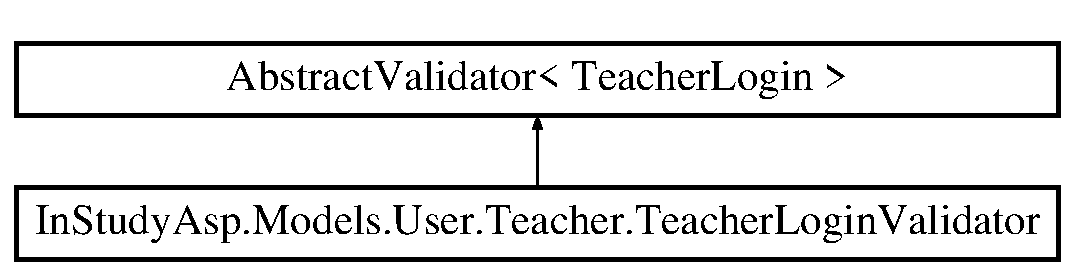
\includegraphics[height=2.000000cm]{class_in_study_asp_1_1_models_1_1_user_1_1_teacher_1_1_teacher_login_validator}
\end{center}
\end{figure}
\subsection*{Public Member Functions}
\begin{DoxyCompactItemize}
\item 
\hyperlink{class_in_study_asp_1_1_models_1_1_user_1_1_teacher_1_1_teacher_login_validator_aab5e05b126ee8333975623630ca3ca7a}{Teacher\+Login\+Validator} ()
\begin{DoxyCompactList}\small\item\em Login validatation rules. \end{DoxyCompactList}\end{DoxyCompactItemize}


\subsection{Detailed Description}
Login validator. 

\subsection{Constructor \& Destructor Documentation}
\mbox{\Hypertarget{class_in_study_asp_1_1_models_1_1_user_1_1_teacher_1_1_teacher_login_validator_aab5e05b126ee8333975623630ca3ca7a}\label{class_in_study_asp_1_1_models_1_1_user_1_1_teacher_1_1_teacher_login_validator_aab5e05b126ee8333975623630ca3ca7a}} 
\index{In\+Study\+Asp\+::\+Models\+::\+User\+::\+Teacher\+::\+Teacher\+Login\+Validator@{In\+Study\+Asp\+::\+Models\+::\+User\+::\+Teacher\+::\+Teacher\+Login\+Validator}!Teacher\+Login\+Validator@{Teacher\+Login\+Validator}}
\index{Teacher\+Login\+Validator@{Teacher\+Login\+Validator}!In\+Study\+Asp\+::\+Models\+::\+User\+::\+Teacher\+::\+Teacher\+Login\+Validator@{In\+Study\+Asp\+::\+Models\+::\+User\+::\+Teacher\+::\+Teacher\+Login\+Validator}}
\subsubsection{\texorpdfstring{Teacher\+Login\+Validator()}{TeacherLoginValidator()}}
{\footnotesize\ttfamily In\+Study\+Asp.\+Models.\+User.\+Teacher.\+Teacher\+Login\+Validator.\+Teacher\+Login\+Validator (\begin{DoxyParamCaption}{ }\end{DoxyParamCaption})}



Login validatation rules. 



The documentation for this class was generated from the following file\+:\begin{DoxyCompactItemize}
\item 
D\+:/\+\_\+\+W\+O\+R\+K/\+\_\+\+S\+T\+E\+P/\+In\+Study\+Asp/\+In\+Study\+Asp/\+Models/\+User/\+Teacher/\hyperlink{_teacher_login_8cs}{Teacher\+Login.\+cs}\end{DoxyCompactItemize}

\hypertarget{class_in_study_asp_1_1_models_1_1_user_1_1_teacher_1_1_teacher_metadata}{}\section{In\+Study\+Asp.\+Models.\+User.\+Teacher.\+Teacher\+Metadata Class Reference}
\label{class_in_study_asp_1_1_models_1_1_user_1_1_teacher_1_1_teacher_metadata}\index{In\+Study\+Asp.\+Models.\+User.\+Teacher.\+Teacher\+Metadata@{In\+Study\+Asp.\+Models.\+User.\+Teacher.\+Teacher\+Metadata}}


Methadata for \hyperlink{class_in_study_asp_1_1_models_1_1_user_1_1_teacher_1_1_teacher_registration}{Teacher\+Registration}.  


\subsection*{Properties}
\begin{DoxyCompactItemize}
\item 
string \hyperlink{class_in_study_asp_1_1_models_1_1_user_1_1_teacher_1_1_teacher_metadata_a271e5bda5d1274e87df20ebe4c3c8750}{Firstname}\hspace{0.3cm}{\ttfamily  \mbox{[}get, set\mbox{]}}
\item 
string \hyperlink{class_in_study_asp_1_1_models_1_1_user_1_1_teacher_1_1_teacher_metadata_a417ec653a2ff85635c6e4fbf73f8e7f8}{Lastname}\hspace{0.3cm}{\ttfamily  \mbox{[}get, set\mbox{]}}
\item 
string \hyperlink{class_in_study_asp_1_1_models_1_1_user_1_1_teacher_1_1_teacher_metadata_aca66777b4969dc58a6a0c2345b9c5564}{Email}\hspace{0.3cm}{\ttfamily  \mbox{[}get, set\mbox{]}}
\item 
string \hyperlink{class_in_study_asp_1_1_models_1_1_user_1_1_teacher_1_1_teacher_metadata_a55d4ee9206f6af10cc10623cbffd777c}{Phone}\hspace{0.3cm}{\ttfamily  \mbox{[}get, set\mbox{]}}
\item 
Date\+Time \hyperlink{class_in_study_asp_1_1_models_1_1_user_1_1_teacher_1_1_teacher_metadata_a7b3f5d8fd0a30521c44e104b42e9d80f}{Birthday}\hspace{0.3cm}{\ttfamily  \mbox{[}get, set\mbox{]}}
\item 
Http\+Posted\+File\+Base \hyperlink{class_in_study_asp_1_1_models_1_1_user_1_1_teacher_1_1_teacher_metadata_a6e8df3f14047a4bb9921c1ab7e282ed7}{Avatar}\hspace{0.3cm}{\ttfamily  \mbox{[}get, set\mbox{]}}
\item 
Date\+Time \hyperlink{class_in_study_asp_1_1_models_1_1_user_1_1_teacher_1_1_teacher_metadata_a43720ff8d11f8c1674777a25b9fd868c}{Start}\hspace{0.3cm}{\ttfamily  \mbox{[}get, set\mbox{]}}
\item 
string \hyperlink{class_in_study_asp_1_1_models_1_1_user_1_1_teacher_1_1_teacher_metadata_aaf2462a89eb73ffb19389f7a47d7dde5}{Password}\hspace{0.3cm}{\ttfamily  \mbox{[}get, set\mbox{]}}
\item 
string \hyperlink{class_in_study_asp_1_1_models_1_1_user_1_1_teacher_1_1_teacher_metadata_ab89c96285f519d5e741c4e51a9193412}{Confirm\+Password}\hspace{0.3cm}{\ttfamily  \mbox{[}get, set\mbox{]}}
\end{DoxyCompactItemize}


\subsection{Detailed Description}
Methadata for \hyperlink{class_in_study_asp_1_1_models_1_1_user_1_1_teacher_1_1_teacher_registration}{Teacher\+Registration}. 

\subsection{Property Documentation}
\mbox{\Hypertarget{class_in_study_asp_1_1_models_1_1_user_1_1_teacher_1_1_teacher_metadata_a6e8df3f14047a4bb9921c1ab7e282ed7}\label{class_in_study_asp_1_1_models_1_1_user_1_1_teacher_1_1_teacher_metadata_a6e8df3f14047a4bb9921c1ab7e282ed7}} 
\index{In\+Study\+Asp\+::\+Models\+::\+User\+::\+Teacher\+::\+Teacher\+Metadata@{In\+Study\+Asp\+::\+Models\+::\+User\+::\+Teacher\+::\+Teacher\+Metadata}!Avatar@{Avatar}}
\index{Avatar@{Avatar}!In\+Study\+Asp\+::\+Models\+::\+User\+::\+Teacher\+::\+Teacher\+Metadata@{In\+Study\+Asp\+::\+Models\+::\+User\+::\+Teacher\+::\+Teacher\+Metadata}}
\subsubsection{\texorpdfstring{Avatar}{Avatar}}
{\footnotesize\ttfamily Http\+Posted\+File\+Base In\+Study\+Asp.\+Models.\+User.\+Teacher.\+Teacher\+Metadata.\+Avatar\hspace{0.3cm}{\ttfamily [get]}, {\ttfamily [set]}}

\mbox{\Hypertarget{class_in_study_asp_1_1_models_1_1_user_1_1_teacher_1_1_teacher_metadata_a7b3f5d8fd0a30521c44e104b42e9d80f}\label{class_in_study_asp_1_1_models_1_1_user_1_1_teacher_1_1_teacher_metadata_a7b3f5d8fd0a30521c44e104b42e9d80f}} 
\index{In\+Study\+Asp\+::\+Models\+::\+User\+::\+Teacher\+::\+Teacher\+Metadata@{In\+Study\+Asp\+::\+Models\+::\+User\+::\+Teacher\+::\+Teacher\+Metadata}!Birthday@{Birthday}}
\index{Birthday@{Birthday}!In\+Study\+Asp\+::\+Models\+::\+User\+::\+Teacher\+::\+Teacher\+Metadata@{In\+Study\+Asp\+::\+Models\+::\+User\+::\+Teacher\+::\+Teacher\+Metadata}}
\subsubsection{\texorpdfstring{Birthday}{Birthday}}
{\footnotesize\ttfamily Date\+Time In\+Study\+Asp.\+Models.\+User.\+Teacher.\+Teacher\+Metadata.\+Birthday\hspace{0.3cm}{\ttfamily [get]}, {\ttfamily [set]}}

\mbox{\Hypertarget{class_in_study_asp_1_1_models_1_1_user_1_1_teacher_1_1_teacher_metadata_ab89c96285f519d5e741c4e51a9193412}\label{class_in_study_asp_1_1_models_1_1_user_1_1_teacher_1_1_teacher_metadata_ab89c96285f519d5e741c4e51a9193412}} 
\index{In\+Study\+Asp\+::\+Models\+::\+User\+::\+Teacher\+::\+Teacher\+Metadata@{In\+Study\+Asp\+::\+Models\+::\+User\+::\+Teacher\+::\+Teacher\+Metadata}!Confirm\+Password@{Confirm\+Password}}
\index{Confirm\+Password@{Confirm\+Password}!In\+Study\+Asp\+::\+Models\+::\+User\+::\+Teacher\+::\+Teacher\+Metadata@{In\+Study\+Asp\+::\+Models\+::\+User\+::\+Teacher\+::\+Teacher\+Metadata}}
\subsubsection{\texorpdfstring{Confirm\+Password}{ConfirmPassword}}
{\footnotesize\ttfamily string In\+Study\+Asp.\+Models.\+User.\+Teacher.\+Teacher\+Metadata.\+Confirm\+Password\hspace{0.3cm}{\ttfamily [get]}, {\ttfamily [set]}}

\mbox{\Hypertarget{class_in_study_asp_1_1_models_1_1_user_1_1_teacher_1_1_teacher_metadata_aca66777b4969dc58a6a0c2345b9c5564}\label{class_in_study_asp_1_1_models_1_1_user_1_1_teacher_1_1_teacher_metadata_aca66777b4969dc58a6a0c2345b9c5564}} 
\index{In\+Study\+Asp\+::\+Models\+::\+User\+::\+Teacher\+::\+Teacher\+Metadata@{In\+Study\+Asp\+::\+Models\+::\+User\+::\+Teacher\+::\+Teacher\+Metadata}!Email@{Email}}
\index{Email@{Email}!In\+Study\+Asp\+::\+Models\+::\+User\+::\+Teacher\+::\+Teacher\+Metadata@{In\+Study\+Asp\+::\+Models\+::\+User\+::\+Teacher\+::\+Teacher\+Metadata}}
\subsubsection{\texorpdfstring{Email}{Email}}
{\footnotesize\ttfamily string In\+Study\+Asp.\+Models.\+User.\+Teacher.\+Teacher\+Metadata.\+Email\hspace{0.3cm}{\ttfamily [get]}, {\ttfamily [set]}}

\mbox{\Hypertarget{class_in_study_asp_1_1_models_1_1_user_1_1_teacher_1_1_teacher_metadata_a271e5bda5d1274e87df20ebe4c3c8750}\label{class_in_study_asp_1_1_models_1_1_user_1_1_teacher_1_1_teacher_metadata_a271e5bda5d1274e87df20ebe4c3c8750}} 
\index{In\+Study\+Asp\+::\+Models\+::\+User\+::\+Teacher\+::\+Teacher\+Metadata@{In\+Study\+Asp\+::\+Models\+::\+User\+::\+Teacher\+::\+Teacher\+Metadata}!Firstname@{Firstname}}
\index{Firstname@{Firstname}!In\+Study\+Asp\+::\+Models\+::\+User\+::\+Teacher\+::\+Teacher\+Metadata@{In\+Study\+Asp\+::\+Models\+::\+User\+::\+Teacher\+::\+Teacher\+Metadata}}
\subsubsection{\texorpdfstring{Firstname}{Firstname}}
{\footnotesize\ttfamily string In\+Study\+Asp.\+Models.\+User.\+Teacher.\+Teacher\+Metadata.\+Firstname\hspace{0.3cm}{\ttfamily [get]}, {\ttfamily [set]}}

\mbox{\Hypertarget{class_in_study_asp_1_1_models_1_1_user_1_1_teacher_1_1_teacher_metadata_a417ec653a2ff85635c6e4fbf73f8e7f8}\label{class_in_study_asp_1_1_models_1_1_user_1_1_teacher_1_1_teacher_metadata_a417ec653a2ff85635c6e4fbf73f8e7f8}} 
\index{In\+Study\+Asp\+::\+Models\+::\+User\+::\+Teacher\+::\+Teacher\+Metadata@{In\+Study\+Asp\+::\+Models\+::\+User\+::\+Teacher\+::\+Teacher\+Metadata}!Lastname@{Lastname}}
\index{Lastname@{Lastname}!In\+Study\+Asp\+::\+Models\+::\+User\+::\+Teacher\+::\+Teacher\+Metadata@{In\+Study\+Asp\+::\+Models\+::\+User\+::\+Teacher\+::\+Teacher\+Metadata}}
\subsubsection{\texorpdfstring{Lastname}{Lastname}}
{\footnotesize\ttfamily string In\+Study\+Asp.\+Models.\+User.\+Teacher.\+Teacher\+Metadata.\+Lastname\hspace{0.3cm}{\ttfamily [get]}, {\ttfamily [set]}}

\mbox{\Hypertarget{class_in_study_asp_1_1_models_1_1_user_1_1_teacher_1_1_teacher_metadata_aaf2462a89eb73ffb19389f7a47d7dde5}\label{class_in_study_asp_1_1_models_1_1_user_1_1_teacher_1_1_teacher_metadata_aaf2462a89eb73ffb19389f7a47d7dde5}} 
\index{In\+Study\+Asp\+::\+Models\+::\+User\+::\+Teacher\+::\+Teacher\+Metadata@{In\+Study\+Asp\+::\+Models\+::\+User\+::\+Teacher\+::\+Teacher\+Metadata}!Password@{Password}}
\index{Password@{Password}!In\+Study\+Asp\+::\+Models\+::\+User\+::\+Teacher\+::\+Teacher\+Metadata@{In\+Study\+Asp\+::\+Models\+::\+User\+::\+Teacher\+::\+Teacher\+Metadata}}
\subsubsection{\texorpdfstring{Password}{Password}}
{\footnotesize\ttfamily string In\+Study\+Asp.\+Models.\+User.\+Teacher.\+Teacher\+Metadata.\+Password\hspace{0.3cm}{\ttfamily [get]}, {\ttfamily [set]}}

\mbox{\Hypertarget{class_in_study_asp_1_1_models_1_1_user_1_1_teacher_1_1_teacher_metadata_a55d4ee9206f6af10cc10623cbffd777c}\label{class_in_study_asp_1_1_models_1_1_user_1_1_teacher_1_1_teacher_metadata_a55d4ee9206f6af10cc10623cbffd777c}} 
\index{In\+Study\+Asp\+::\+Models\+::\+User\+::\+Teacher\+::\+Teacher\+Metadata@{In\+Study\+Asp\+::\+Models\+::\+User\+::\+Teacher\+::\+Teacher\+Metadata}!Phone@{Phone}}
\index{Phone@{Phone}!In\+Study\+Asp\+::\+Models\+::\+User\+::\+Teacher\+::\+Teacher\+Metadata@{In\+Study\+Asp\+::\+Models\+::\+User\+::\+Teacher\+::\+Teacher\+Metadata}}
\subsubsection{\texorpdfstring{Phone}{Phone}}
{\footnotesize\ttfamily string In\+Study\+Asp.\+Models.\+User.\+Teacher.\+Teacher\+Metadata.\+Phone\hspace{0.3cm}{\ttfamily [get]}, {\ttfamily [set]}}

\mbox{\Hypertarget{class_in_study_asp_1_1_models_1_1_user_1_1_teacher_1_1_teacher_metadata_a43720ff8d11f8c1674777a25b9fd868c}\label{class_in_study_asp_1_1_models_1_1_user_1_1_teacher_1_1_teacher_metadata_a43720ff8d11f8c1674777a25b9fd868c}} 
\index{In\+Study\+Asp\+::\+Models\+::\+User\+::\+Teacher\+::\+Teacher\+Metadata@{In\+Study\+Asp\+::\+Models\+::\+User\+::\+Teacher\+::\+Teacher\+Metadata}!Start@{Start}}
\index{Start@{Start}!In\+Study\+Asp\+::\+Models\+::\+User\+::\+Teacher\+::\+Teacher\+Metadata@{In\+Study\+Asp\+::\+Models\+::\+User\+::\+Teacher\+::\+Teacher\+Metadata}}
\subsubsection{\texorpdfstring{Start}{Start}}
{\footnotesize\ttfamily Date\+Time In\+Study\+Asp.\+Models.\+User.\+Teacher.\+Teacher\+Metadata.\+Start\hspace{0.3cm}{\ttfamily [get]}, {\ttfamily [set]}}



The documentation for this class was generated from the following file\+:\begin{DoxyCompactItemize}
\item 
D\+:/\+\_\+\+W\+O\+R\+K/\+\_\+\+S\+T\+E\+P/\+In\+Study\+Asp/\+In\+Study\+Asp/\+Models/\+User/\+Teacher/\hyperlink{_teacher_registration_8cs}{Teacher\+Registration.\+cs}\end{DoxyCompactItemize}

\hypertarget{class_in_study_asp_1_1_models_1_1_user_1_1_teacher_1_1_teacher_registration}{}\section{In\+Study\+Asp.\+Models.\+User.\+Teacher.\+Teacher\+Registration Class Reference}
\label{class_in_study_asp_1_1_models_1_1_user_1_1_teacher_1_1_teacher_registration}\index{In\+Study\+Asp.\+Models.\+User.\+Teacher.\+Teacher\+Registration@{In\+Study\+Asp.\+Models.\+User.\+Teacher.\+Teacher\+Registration}}


View\+Model for teacher\+Registration.  


\subsection*{Public Member Functions}
\begin{DoxyCompactItemize}
\item 
bool \hyperlink{class_in_study_asp_1_1_models_1_1_user_1_1_teacher_1_1_teacher_registration_aa32defbc6273f2a084d3ec9c1f5fec0a}{Phone\+Exist} ()
\item 
void \hyperlink{class_in_study_asp_1_1_models_1_1_user_1_1_teacher_1_1_teacher_registration_ad2db85099f5b797b8a9a3b304d5604fe}{Save\+To\+Database} (\hyperlink{class_e_f_oracle_1_1_model_1_1db_context}{E\+F\+Oracle.\+Model.\+db\+Context} \hyperlink{class_e_f_oracle_1_1_model_1_1db_context}{db\+Context})
\begin{DoxyCompactList}\small\item\em Saving registration data to db. \end{DoxyCompactList}\end{DoxyCompactItemize}
\subsection*{Properties}
\begin{DoxyCompactItemize}
\item 
string \hyperlink{class_in_study_asp_1_1_models_1_1_user_1_1_teacher_1_1_teacher_registration_a22859db83f2ede97bdc3cf142a2953dd}{Firstname}\hspace{0.3cm}{\ttfamily  \mbox{[}get, set\mbox{]}}
\item 
string \hyperlink{class_in_study_asp_1_1_models_1_1_user_1_1_teacher_1_1_teacher_registration_ae194bb95abc77b2407fc7fa075fb4b65}{Lastname}\hspace{0.3cm}{\ttfamily  \mbox{[}get, set\mbox{]}}
\item 
string \hyperlink{class_in_study_asp_1_1_models_1_1_user_1_1_teacher_1_1_teacher_registration_a1720a6da6108baa8a8e353dd4708029d}{Email}\hspace{0.3cm}{\ttfamily  \mbox{[}get, set\mbox{]}}
\item 
string \hyperlink{class_in_study_asp_1_1_models_1_1_user_1_1_teacher_1_1_teacher_registration_a4bbef08cff05bc5da059062fc912e9c4}{Phone}\hspace{0.3cm}{\ttfamily  \mbox{[}get, set\mbox{]}}
\item 
Date\+Time \hyperlink{class_in_study_asp_1_1_models_1_1_user_1_1_teacher_1_1_teacher_registration_a28b978235dc87d60752e4b56bde36092}{Birthday}\hspace{0.3cm}{\ttfamily  \mbox{[}get, set\mbox{]}}
\item 
Http\+Posted\+File\+Base \hyperlink{class_in_study_asp_1_1_models_1_1_user_1_1_teacher_1_1_teacher_registration_ae6036d0740c0a5e9fd842548414f14db}{Avatar}\hspace{0.3cm}{\ttfamily  \mbox{[}get, set\mbox{]}}
\item 
Date\+Time \hyperlink{class_in_study_asp_1_1_models_1_1_user_1_1_teacher_1_1_teacher_registration_a4a3c193dddb92594f9ad5cd24040dbb3}{Start}\hspace{0.3cm}{\ttfamily  \mbox{[}get, set\mbox{]}}
\item 
string \hyperlink{class_in_study_asp_1_1_models_1_1_user_1_1_teacher_1_1_teacher_registration_a2e2d5af0d73b8711f41beee478784a50}{Password}\hspace{0.3cm}{\ttfamily  \mbox{[}get, set\mbox{]}}
\item 
string \hyperlink{class_in_study_asp_1_1_models_1_1_user_1_1_teacher_1_1_teacher_registration_a1478cc3f2a59a17dd8674510bfb28e71}{Confirm\+Password}\hspace{0.3cm}{\ttfamily  \mbox{[}get, set\mbox{]}}
\item 
string \hyperlink{class_in_study_asp_1_1_models_1_1_user_1_1_teacher_1_1_teacher_registration_afc7014fd0b5720e1611e747fddfa89bd}{Activation\+Code}\hspace{0.3cm}{\ttfamily  \mbox{[}get, set\mbox{]}}
\end{DoxyCompactItemize}
\subsection*{Private Member Functions}
\begin{DoxyCompactItemize}
\item 
string \hyperlink{class_in_study_asp_1_1_models_1_1_user_1_1_teacher_1_1_teacher_registration_a045ff1afe4855128eabe0e258029c741}{Hash} (string pass)
\begin{DoxyCompactList}\small\item\em Hashing password. \end{DoxyCompactList}\end{DoxyCompactItemize}


\subsection{Detailed Description}
View\+Model for teacher\+Registration. 

\subsection{Member Function Documentation}
\mbox{\Hypertarget{class_in_study_asp_1_1_models_1_1_user_1_1_teacher_1_1_teacher_registration_a045ff1afe4855128eabe0e258029c741}\label{class_in_study_asp_1_1_models_1_1_user_1_1_teacher_1_1_teacher_registration_a045ff1afe4855128eabe0e258029c741}} 
\index{In\+Study\+Asp\+::\+Models\+::\+User\+::\+Teacher\+::\+Teacher\+Registration@{In\+Study\+Asp\+::\+Models\+::\+User\+::\+Teacher\+::\+Teacher\+Registration}!Hash@{Hash}}
\index{Hash@{Hash}!In\+Study\+Asp\+::\+Models\+::\+User\+::\+Teacher\+::\+Teacher\+Registration@{In\+Study\+Asp\+::\+Models\+::\+User\+::\+Teacher\+::\+Teacher\+Registration}}
\subsubsection{\texorpdfstring{Hash()}{Hash()}}
{\footnotesize\ttfamily string In\+Study\+Asp.\+Models.\+User.\+Teacher.\+Teacher\+Registration.\+Hash (\begin{DoxyParamCaption}\item[{string}]{pass }\end{DoxyParamCaption})\hspace{0.3cm}{\ttfamily [private]}}



Hashing password. 

\mbox{\Hypertarget{class_in_study_asp_1_1_models_1_1_user_1_1_teacher_1_1_teacher_registration_aa32defbc6273f2a084d3ec9c1f5fec0a}\label{class_in_study_asp_1_1_models_1_1_user_1_1_teacher_1_1_teacher_registration_aa32defbc6273f2a084d3ec9c1f5fec0a}} 
\index{In\+Study\+Asp\+::\+Models\+::\+User\+::\+Teacher\+::\+Teacher\+Registration@{In\+Study\+Asp\+::\+Models\+::\+User\+::\+Teacher\+::\+Teacher\+Registration}!Phone\+Exist@{Phone\+Exist}}
\index{Phone\+Exist@{Phone\+Exist}!In\+Study\+Asp\+::\+Models\+::\+User\+::\+Teacher\+::\+Teacher\+Registration@{In\+Study\+Asp\+::\+Models\+::\+User\+::\+Teacher\+::\+Teacher\+Registration}}
\subsubsection{\texorpdfstring{Phone\+Exist()}{PhoneExist()}}
{\footnotesize\ttfamily bool In\+Study\+Asp.\+Models.\+User.\+Teacher.\+Teacher\+Registration.\+Phone\+Exist (\begin{DoxyParamCaption}{ }\end{DoxyParamCaption})}

\mbox{\Hypertarget{class_in_study_asp_1_1_models_1_1_user_1_1_teacher_1_1_teacher_registration_ad2db85099f5b797b8a9a3b304d5604fe}\label{class_in_study_asp_1_1_models_1_1_user_1_1_teacher_1_1_teacher_registration_ad2db85099f5b797b8a9a3b304d5604fe}} 
\index{In\+Study\+Asp\+::\+Models\+::\+User\+::\+Teacher\+::\+Teacher\+Registration@{In\+Study\+Asp\+::\+Models\+::\+User\+::\+Teacher\+::\+Teacher\+Registration}!Save\+To\+Database@{Save\+To\+Database}}
\index{Save\+To\+Database@{Save\+To\+Database}!In\+Study\+Asp\+::\+Models\+::\+User\+::\+Teacher\+::\+Teacher\+Registration@{In\+Study\+Asp\+::\+Models\+::\+User\+::\+Teacher\+::\+Teacher\+Registration}}
\subsubsection{\texorpdfstring{Save\+To\+Database()}{SaveToDatabase()}}
{\footnotesize\ttfamily void In\+Study\+Asp.\+Models.\+User.\+Teacher.\+Teacher\+Registration.\+Save\+To\+Database (\begin{DoxyParamCaption}\item[{\hyperlink{class_e_f_oracle_1_1_model_1_1db_context}{E\+F\+Oracle.\+Model.\+db\+Context}}]{db\+Context }\end{DoxyParamCaption})}



Saving registration data to db. 



\subsection{Property Documentation}
\mbox{\Hypertarget{class_in_study_asp_1_1_models_1_1_user_1_1_teacher_1_1_teacher_registration_afc7014fd0b5720e1611e747fddfa89bd}\label{class_in_study_asp_1_1_models_1_1_user_1_1_teacher_1_1_teacher_registration_afc7014fd0b5720e1611e747fddfa89bd}} 
\index{In\+Study\+Asp\+::\+Models\+::\+User\+::\+Teacher\+::\+Teacher\+Registration@{In\+Study\+Asp\+::\+Models\+::\+User\+::\+Teacher\+::\+Teacher\+Registration}!Activation\+Code@{Activation\+Code}}
\index{Activation\+Code@{Activation\+Code}!In\+Study\+Asp\+::\+Models\+::\+User\+::\+Teacher\+::\+Teacher\+Registration@{In\+Study\+Asp\+::\+Models\+::\+User\+::\+Teacher\+::\+Teacher\+Registration}}
\subsubsection{\texorpdfstring{Activation\+Code}{ActivationCode}}
{\footnotesize\ttfamily string In\+Study\+Asp.\+Models.\+User.\+Teacher.\+Teacher\+Registration.\+Activation\+Code\hspace{0.3cm}{\ttfamily [get]}, {\ttfamily [set]}}

\mbox{\Hypertarget{class_in_study_asp_1_1_models_1_1_user_1_1_teacher_1_1_teacher_registration_ae6036d0740c0a5e9fd842548414f14db}\label{class_in_study_asp_1_1_models_1_1_user_1_1_teacher_1_1_teacher_registration_ae6036d0740c0a5e9fd842548414f14db}} 
\index{In\+Study\+Asp\+::\+Models\+::\+User\+::\+Teacher\+::\+Teacher\+Registration@{In\+Study\+Asp\+::\+Models\+::\+User\+::\+Teacher\+::\+Teacher\+Registration}!Avatar@{Avatar}}
\index{Avatar@{Avatar}!In\+Study\+Asp\+::\+Models\+::\+User\+::\+Teacher\+::\+Teacher\+Registration@{In\+Study\+Asp\+::\+Models\+::\+User\+::\+Teacher\+::\+Teacher\+Registration}}
\subsubsection{\texorpdfstring{Avatar}{Avatar}}
{\footnotesize\ttfamily Http\+Posted\+File\+Base In\+Study\+Asp.\+Models.\+User.\+Teacher.\+Teacher\+Registration.\+Avatar\hspace{0.3cm}{\ttfamily [get]}, {\ttfamily [set]}}

\mbox{\Hypertarget{class_in_study_asp_1_1_models_1_1_user_1_1_teacher_1_1_teacher_registration_a28b978235dc87d60752e4b56bde36092}\label{class_in_study_asp_1_1_models_1_1_user_1_1_teacher_1_1_teacher_registration_a28b978235dc87d60752e4b56bde36092}} 
\index{In\+Study\+Asp\+::\+Models\+::\+User\+::\+Teacher\+::\+Teacher\+Registration@{In\+Study\+Asp\+::\+Models\+::\+User\+::\+Teacher\+::\+Teacher\+Registration}!Birthday@{Birthday}}
\index{Birthday@{Birthday}!In\+Study\+Asp\+::\+Models\+::\+User\+::\+Teacher\+::\+Teacher\+Registration@{In\+Study\+Asp\+::\+Models\+::\+User\+::\+Teacher\+::\+Teacher\+Registration}}
\subsubsection{\texorpdfstring{Birthday}{Birthday}}
{\footnotesize\ttfamily Date\+Time In\+Study\+Asp.\+Models.\+User.\+Teacher.\+Teacher\+Registration.\+Birthday\hspace{0.3cm}{\ttfamily [get]}, {\ttfamily [set]}}

\mbox{\Hypertarget{class_in_study_asp_1_1_models_1_1_user_1_1_teacher_1_1_teacher_registration_a1478cc3f2a59a17dd8674510bfb28e71}\label{class_in_study_asp_1_1_models_1_1_user_1_1_teacher_1_1_teacher_registration_a1478cc3f2a59a17dd8674510bfb28e71}} 
\index{In\+Study\+Asp\+::\+Models\+::\+User\+::\+Teacher\+::\+Teacher\+Registration@{In\+Study\+Asp\+::\+Models\+::\+User\+::\+Teacher\+::\+Teacher\+Registration}!Confirm\+Password@{Confirm\+Password}}
\index{Confirm\+Password@{Confirm\+Password}!In\+Study\+Asp\+::\+Models\+::\+User\+::\+Teacher\+::\+Teacher\+Registration@{In\+Study\+Asp\+::\+Models\+::\+User\+::\+Teacher\+::\+Teacher\+Registration}}
\subsubsection{\texorpdfstring{Confirm\+Password}{ConfirmPassword}}
{\footnotesize\ttfamily string In\+Study\+Asp.\+Models.\+User.\+Teacher.\+Teacher\+Registration.\+Confirm\+Password\hspace{0.3cm}{\ttfamily [get]}, {\ttfamily [set]}}

\mbox{\Hypertarget{class_in_study_asp_1_1_models_1_1_user_1_1_teacher_1_1_teacher_registration_a1720a6da6108baa8a8e353dd4708029d}\label{class_in_study_asp_1_1_models_1_1_user_1_1_teacher_1_1_teacher_registration_a1720a6da6108baa8a8e353dd4708029d}} 
\index{In\+Study\+Asp\+::\+Models\+::\+User\+::\+Teacher\+::\+Teacher\+Registration@{In\+Study\+Asp\+::\+Models\+::\+User\+::\+Teacher\+::\+Teacher\+Registration}!Email@{Email}}
\index{Email@{Email}!In\+Study\+Asp\+::\+Models\+::\+User\+::\+Teacher\+::\+Teacher\+Registration@{In\+Study\+Asp\+::\+Models\+::\+User\+::\+Teacher\+::\+Teacher\+Registration}}
\subsubsection{\texorpdfstring{Email}{Email}}
{\footnotesize\ttfamily string In\+Study\+Asp.\+Models.\+User.\+Teacher.\+Teacher\+Registration.\+Email\hspace{0.3cm}{\ttfamily [get]}, {\ttfamily [set]}}

\mbox{\Hypertarget{class_in_study_asp_1_1_models_1_1_user_1_1_teacher_1_1_teacher_registration_a22859db83f2ede97bdc3cf142a2953dd}\label{class_in_study_asp_1_1_models_1_1_user_1_1_teacher_1_1_teacher_registration_a22859db83f2ede97bdc3cf142a2953dd}} 
\index{In\+Study\+Asp\+::\+Models\+::\+User\+::\+Teacher\+::\+Teacher\+Registration@{In\+Study\+Asp\+::\+Models\+::\+User\+::\+Teacher\+::\+Teacher\+Registration}!Firstname@{Firstname}}
\index{Firstname@{Firstname}!In\+Study\+Asp\+::\+Models\+::\+User\+::\+Teacher\+::\+Teacher\+Registration@{In\+Study\+Asp\+::\+Models\+::\+User\+::\+Teacher\+::\+Teacher\+Registration}}
\subsubsection{\texorpdfstring{Firstname}{Firstname}}
{\footnotesize\ttfamily string In\+Study\+Asp.\+Models.\+User.\+Teacher.\+Teacher\+Registration.\+Firstname\hspace{0.3cm}{\ttfamily [get]}, {\ttfamily [set]}}

\mbox{\Hypertarget{class_in_study_asp_1_1_models_1_1_user_1_1_teacher_1_1_teacher_registration_ae194bb95abc77b2407fc7fa075fb4b65}\label{class_in_study_asp_1_1_models_1_1_user_1_1_teacher_1_1_teacher_registration_ae194bb95abc77b2407fc7fa075fb4b65}} 
\index{In\+Study\+Asp\+::\+Models\+::\+User\+::\+Teacher\+::\+Teacher\+Registration@{In\+Study\+Asp\+::\+Models\+::\+User\+::\+Teacher\+::\+Teacher\+Registration}!Lastname@{Lastname}}
\index{Lastname@{Lastname}!In\+Study\+Asp\+::\+Models\+::\+User\+::\+Teacher\+::\+Teacher\+Registration@{In\+Study\+Asp\+::\+Models\+::\+User\+::\+Teacher\+::\+Teacher\+Registration}}
\subsubsection{\texorpdfstring{Lastname}{Lastname}}
{\footnotesize\ttfamily string In\+Study\+Asp.\+Models.\+User.\+Teacher.\+Teacher\+Registration.\+Lastname\hspace{0.3cm}{\ttfamily [get]}, {\ttfamily [set]}}

\mbox{\Hypertarget{class_in_study_asp_1_1_models_1_1_user_1_1_teacher_1_1_teacher_registration_a2e2d5af0d73b8711f41beee478784a50}\label{class_in_study_asp_1_1_models_1_1_user_1_1_teacher_1_1_teacher_registration_a2e2d5af0d73b8711f41beee478784a50}} 
\index{In\+Study\+Asp\+::\+Models\+::\+User\+::\+Teacher\+::\+Teacher\+Registration@{In\+Study\+Asp\+::\+Models\+::\+User\+::\+Teacher\+::\+Teacher\+Registration}!Password@{Password}}
\index{Password@{Password}!In\+Study\+Asp\+::\+Models\+::\+User\+::\+Teacher\+::\+Teacher\+Registration@{In\+Study\+Asp\+::\+Models\+::\+User\+::\+Teacher\+::\+Teacher\+Registration}}
\subsubsection{\texorpdfstring{Password}{Password}}
{\footnotesize\ttfamily string In\+Study\+Asp.\+Models.\+User.\+Teacher.\+Teacher\+Registration.\+Password\hspace{0.3cm}{\ttfamily [get]}, {\ttfamily [set]}}

\mbox{\Hypertarget{class_in_study_asp_1_1_models_1_1_user_1_1_teacher_1_1_teacher_registration_a4bbef08cff05bc5da059062fc912e9c4}\label{class_in_study_asp_1_1_models_1_1_user_1_1_teacher_1_1_teacher_registration_a4bbef08cff05bc5da059062fc912e9c4}} 
\index{In\+Study\+Asp\+::\+Models\+::\+User\+::\+Teacher\+::\+Teacher\+Registration@{In\+Study\+Asp\+::\+Models\+::\+User\+::\+Teacher\+::\+Teacher\+Registration}!Phone@{Phone}}
\index{Phone@{Phone}!In\+Study\+Asp\+::\+Models\+::\+User\+::\+Teacher\+::\+Teacher\+Registration@{In\+Study\+Asp\+::\+Models\+::\+User\+::\+Teacher\+::\+Teacher\+Registration}}
\subsubsection{\texorpdfstring{Phone}{Phone}}
{\footnotesize\ttfamily string In\+Study\+Asp.\+Models.\+User.\+Teacher.\+Teacher\+Registration.\+Phone\hspace{0.3cm}{\ttfamily [get]}, {\ttfamily [set]}}

\mbox{\Hypertarget{class_in_study_asp_1_1_models_1_1_user_1_1_teacher_1_1_teacher_registration_a4a3c193dddb92594f9ad5cd24040dbb3}\label{class_in_study_asp_1_1_models_1_1_user_1_1_teacher_1_1_teacher_registration_a4a3c193dddb92594f9ad5cd24040dbb3}} 
\index{In\+Study\+Asp\+::\+Models\+::\+User\+::\+Teacher\+::\+Teacher\+Registration@{In\+Study\+Asp\+::\+Models\+::\+User\+::\+Teacher\+::\+Teacher\+Registration}!Start@{Start}}
\index{Start@{Start}!In\+Study\+Asp\+::\+Models\+::\+User\+::\+Teacher\+::\+Teacher\+Registration@{In\+Study\+Asp\+::\+Models\+::\+User\+::\+Teacher\+::\+Teacher\+Registration}}
\subsubsection{\texorpdfstring{Start}{Start}}
{\footnotesize\ttfamily Date\+Time In\+Study\+Asp.\+Models.\+User.\+Teacher.\+Teacher\+Registration.\+Start\hspace{0.3cm}{\ttfamily [get]}, {\ttfamily [set]}}



The documentation for this class was generated from the following file\+:\begin{DoxyCompactItemize}
\item 
D\+:/\+\_\+\+W\+O\+R\+K/\+\_\+\+S\+T\+E\+P/\+In\+Study\+Asp/\+In\+Study\+Asp/\+Models/\+User/\+Teacher/\hyperlink{_teacher_registration_8cs}{Teacher\+Registration.\+cs}\end{DoxyCompactItemize}

\hypertarget{class_in_study_asp_1_1_controllers_1_1_user_1_1_teacher_1_1_teacher_registration_controller}{}\section{In\+Study\+Asp.\+Controllers.\+User.\+Teacher.\+Teacher\+Registration\+Controller Class Reference}
\label{class_in_study_asp_1_1_controllers_1_1_user_1_1_teacher_1_1_teacher_registration_controller}\index{In\+Study\+Asp.\+Controllers.\+User.\+Teacher.\+Teacher\+Registration\+Controller@{In\+Study\+Asp.\+Controllers.\+User.\+Teacher.\+Teacher\+Registration\+Controller}}
Inheritance diagram for In\+Study\+Asp.\+Controllers.\+User.\+Teacher.\+Teacher\+Registration\+Controller\+:\begin{figure}[H]
\begin{center}
\leavevmode
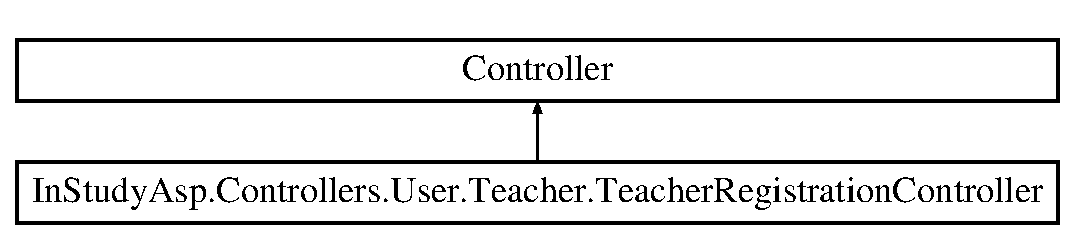
\includegraphics[height=2.000000cm]{class_in_study_asp_1_1_controllers_1_1_user_1_1_teacher_1_1_teacher_registration_controller}
\end{center}
\end{figure}
\subsection*{Public Member Functions}
\begin{DoxyCompactItemize}
\item 
Action\+Result \hyperlink{class_in_study_asp_1_1_controllers_1_1_user_1_1_teacher_1_1_teacher_registration_controller_afb1dcb3b2a2511cf4fe4a129909ecbd2}{Registration} ()
\item 
Action\+Result \hyperlink{class_in_study_asp_1_1_controllers_1_1_user_1_1_teacher_1_1_teacher_registration_controller_a3ea2029bfd432a4f608d472569fea93f}{Registration} (\mbox{[}Bind(Exclude=\char`\"{}Is\+Email\+Veryfied,Activation\+Code\char`\"{})\mbox{]} Teacher\+Registration teacher\+Registration)
\item 
Action\+Result \hyperlink{class_in_study_asp_1_1_controllers_1_1_user_1_1_teacher_1_1_teacher_registration_controller_a722d8fc6094e16cddacd6318ee195de2}{Verify\+Account} (string id)
\item 
Action\+Result \hyperlink{class_in_study_asp_1_1_controllers_1_1_user_1_1_teacher_1_1_teacher_registration_controller_a8f5b53c1ab9d03840054ee43be913d38}{Login} ()
\item 
Action\+Result \hyperlink{class_in_study_asp_1_1_controllers_1_1_user_1_1_teacher_1_1_teacher_registration_controller_a30ca9e7d8bc106277af9148a2ede3280}{Login} (\hyperlink{class_in_study_asp_1_1_models_1_1_user_1_1_teacher_1_1_teacher_login}{Teacher\+Login} login, string return\+Url=\char`\"{}\char`\"{})
\item 
Action\+Result \hyperlink{class_in_study_asp_1_1_controllers_1_1_user_1_1_teacher_1_1_teacher_registration_controller_a6d4a0d17fe318c5c0f1df4437dbac597}{Logout} ()
\end{DoxyCompactItemize}


\subsection{Detailed Description}
contains all user idenification actions provides Registration, Veryfiaccount, Login, Logout actions 

\subsection{Member Function Documentation}
\mbox{\Hypertarget{class_in_study_asp_1_1_controllers_1_1_user_1_1_teacher_1_1_teacher_registration_controller_a8f5b53c1ab9d03840054ee43be913d38}\label{class_in_study_asp_1_1_controllers_1_1_user_1_1_teacher_1_1_teacher_registration_controller_a8f5b53c1ab9d03840054ee43be913d38}} 
\index{In\+Study\+Asp\+::\+Controllers\+::\+User\+::\+Teacher\+::\+Teacher\+Registration\+Controller@{In\+Study\+Asp\+::\+Controllers\+::\+User\+::\+Teacher\+::\+Teacher\+Registration\+Controller}!Login@{Login}}
\index{Login@{Login}!In\+Study\+Asp\+::\+Controllers\+::\+User\+::\+Teacher\+::\+Teacher\+Registration\+Controller@{In\+Study\+Asp\+::\+Controllers\+::\+User\+::\+Teacher\+::\+Teacher\+Registration\+Controller}}
\subsubsection{\texorpdfstring{Login()}{Login()}\hspace{0.1cm}{\footnotesize\ttfamily [1/2]}}
{\footnotesize\ttfamily Action\+Result In\+Study\+Asp.\+Controllers.\+User.\+Teacher.\+Teacher\+Registration\+Controller.\+Login (\begin{DoxyParamCaption}{ }\end{DoxyParamCaption})}

\textbackslash{} Processing Login Get \mbox{\Hypertarget{class_in_study_asp_1_1_controllers_1_1_user_1_1_teacher_1_1_teacher_registration_controller_a30ca9e7d8bc106277af9148a2ede3280}\label{class_in_study_asp_1_1_controllers_1_1_user_1_1_teacher_1_1_teacher_registration_controller_a30ca9e7d8bc106277af9148a2ede3280}} 
\index{In\+Study\+Asp\+::\+Controllers\+::\+User\+::\+Teacher\+::\+Teacher\+Registration\+Controller@{In\+Study\+Asp\+::\+Controllers\+::\+User\+::\+Teacher\+::\+Teacher\+Registration\+Controller}!Login@{Login}}
\index{Login@{Login}!In\+Study\+Asp\+::\+Controllers\+::\+User\+::\+Teacher\+::\+Teacher\+Registration\+Controller@{In\+Study\+Asp\+::\+Controllers\+::\+User\+::\+Teacher\+::\+Teacher\+Registration\+Controller}}
\subsubsection{\texorpdfstring{Login()}{Login()}\hspace{0.1cm}{\footnotesize\ttfamily [2/2]}}
{\footnotesize\ttfamily Action\+Result In\+Study\+Asp.\+Controllers.\+User.\+Teacher.\+Teacher\+Registration\+Controller.\+Login (\begin{DoxyParamCaption}\item[{\hyperlink{class_in_study_asp_1_1_models_1_1_user_1_1_teacher_1_1_teacher_login}{Teacher\+Login}}]{login,  }\item[{string}]{return\+Url = {\ttfamily \char`\"{}\char`\"{}} }\end{DoxyParamCaption})}

sended login data \mbox{\Hypertarget{class_in_study_asp_1_1_controllers_1_1_user_1_1_teacher_1_1_teacher_registration_controller_a6d4a0d17fe318c5c0f1df4437dbac597}\label{class_in_study_asp_1_1_controllers_1_1_user_1_1_teacher_1_1_teacher_registration_controller_a6d4a0d17fe318c5c0f1df4437dbac597}} 
\index{In\+Study\+Asp\+::\+Controllers\+::\+User\+::\+Teacher\+::\+Teacher\+Registration\+Controller@{In\+Study\+Asp\+::\+Controllers\+::\+User\+::\+Teacher\+::\+Teacher\+Registration\+Controller}!Logout@{Logout}}
\index{Logout@{Logout}!In\+Study\+Asp\+::\+Controllers\+::\+User\+::\+Teacher\+::\+Teacher\+Registration\+Controller@{In\+Study\+Asp\+::\+Controllers\+::\+User\+::\+Teacher\+::\+Teacher\+Registration\+Controller}}
\subsubsection{\texorpdfstring{Logout()}{Logout()}}
{\footnotesize\ttfamily Action\+Result In\+Study\+Asp.\+Controllers.\+User.\+Teacher.\+Teacher\+Registration\+Controller.\+Logout (\begin{DoxyParamCaption}{ }\end{DoxyParamCaption})}

Logout redirect to Action Login \mbox{\Hypertarget{class_in_study_asp_1_1_controllers_1_1_user_1_1_teacher_1_1_teacher_registration_controller_afb1dcb3b2a2511cf4fe4a129909ecbd2}\label{class_in_study_asp_1_1_controllers_1_1_user_1_1_teacher_1_1_teacher_registration_controller_afb1dcb3b2a2511cf4fe4a129909ecbd2}} 
\index{In\+Study\+Asp\+::\+Controllers\+::\+User\+::\+Teacher\+::\+Teacher\+Registration\+Controller@{In\+Study\+Asp\+::\+Controllers\+::\+User\+::\+Teacher\+::\+Teacher\+Registration\+Controller}!Registration@{Registration}}
\index{Registration@{Registration}!In\+Study\+Asp\+::\+Controllers\+::\+User\+::\+Teacher\+::\+Teacher\+Registration\+Controller@{In\+Study\+Asp\+::\+Controllers\+::\+User\+::\+Teacher\+::\+Teacher\+Registration\+Controller}}
\subsubsection{\texorpdfstring{Registration()}{Registration()}\hspace{0.1cm}{\footnotesize\ttfamily [1/2]}}
{\footnotesize\ttfamily Action\+Result In\+Study\+Asp.\+Controllers.\+User.\+Teacher.\+Teacher\+Registration\+Controller.\+Registration (\begin{DoxyParamCaption}{ }\end{DoxyParamCaption})}

G\+ET action id -\/ S\+E\+S\+S\+I\+O\+N\+\_\+\+H\+A\+SH from U\+S\+E\+R\+\_\+\+S\+E\+S\+S\+I\+ON \mbox{\Hypertarget{class_in_study_asp_1_1_controllers_1_1_user_1_1_teacher_1_1_teacher_registration_controller_a3ea2029bfd432a4f608d472569fea93f}\label{class_in_study_asp_1_1_controllers_1_1_user_1_1_teacher_1_1_teacher_registration_controller_a3ea2029bfd432a4f608d472569fea93f}} 
\index{In\+Study\+Asp\+::\+Controllers\+::\+User\+::\+Teacher\+::\+Teacher\+Registration\+Controller@{In\+Study\+Asp\+::\+Controllers\+::\+User\+::\+Teacher\+::\+Teacher\+Registration\+Controller}!Registration@{Registration}}
\index{Registration@{Registration}!In\+Study\+Asp\+::\+Controllers\+::\+User\+::\+Teacher\+::\+Teacher\+Registration\+Controller@{In\+Study\+Asp\+::\+Controllers\+::\+User\+::\+Teacher\+::\+Teacher\+Registration\+Controller}}
\subsubsection{\texorpdfstring{Registration()}{Registration()}\hspace{0.1cm}{\footnotesize\ttfamily [2/2]}}
{\footnotesize\ttfamily Action\+Result In\+Study\+Asp.\+Controllers.\+User.\+Teacher.\+Teacher\+Registration\+Controller.\+Registration (\begin{DoxyParamCaption}\item[{\mbox{[}\+Bind(\+Exclude = \char`\"{}\+Is\+Email\+Veryfied,\+Activation\+Code\char`\"{})\mbox{]} \hyperlink{class_in_study_asp_1_1_models_1_1_user_1_1_teacher_1_1_teacher_registration}{Teacher\+Registration}}]{teacher\+Registration }\end{DoxyParamCaption})}

P\+O\+ST action id -\/ S\+E\+S\+S\+I\+O\+N\+\_\+\+H\+A\+SH from U\+S\+E\+R\+\_\+\+S\+E\+S\+S\+I\+ON \mbox{\Hypertarget{class_in_study_asp_1_1_controllers_1_1_user_1_1_teacher_1_1_teacher_registration_controller_a722d8fc6094e16cddacd6318ee195de2}\label{class_in_study_asp_1_1_controllers_1_1_user_1_1_teacher_1_1_teacher_registration_controller_a722d8fc6094e16cddacd6318ee195de2}} 
\index{In\+Study\+Asp\+::\+Controllers\+::\+User\+::\+Teacher\+::\+Teacher\+Registration\+Controller@{In\+Study\+Asp\+::\+Controllers\+::\+User\+::\+Teacher\+::\+Teacher\+Registration\+Controller}!Verify\+Account@{Verify\+Account}}
\index{Verify\+Account@{Verify\+Account}!In\+Study\+Asp\+::\+Controllers\+::\+User\+::\+Teacher\+::\+Teacher\+Registration\+Controller@{In\+Study\+Asp\+::\+Controllers\+::\+User\+::\+Teacher\+::\+Teacher\+Registration\+Controller}}
\subsubsection{\texorpdfstring{Verify\+Account()}{VerifyAccount()}}
{\footnotesize\ttfamily Action\+Result In\+Study\+Asp.\+Controllers.\+User.\+Teacher.\+Teacher\+Registration\+Controller.\+Verify\+Account (\begin{DoxyParamCaption}\item[{string}]{id }\end{DoxyParamCaption})}

Account, set mark U\+S\+E\+R.\+U\+S\+E\+R\+\_\+\+I\+S\+\_\+\+A\+C\+T\+I\+V\+A\+T\+ED = -\/1 id -\/ U\+S\+E\+R\+\_\+\+S\+E\+S\+S\+I\+O\+N.\+S\+E\+S\+S\+I\+O\+N\+\_\+\+H\+A\+SH 

The documentation for this class was generated from the following file\+:\begin{DoxyCompactItemize}
\item 
D\+:/\+\_\+\+W\+O\+R\+K/\+\_\+\+S\+T\+E\+P/\+In\+Study\+Asp/\+In\+Study\+Asp/\+Controllers/\+User/\+Teacher/\hyperlink{_teacher_registration_controller_8cs}{Teacher\+Registration\+Controller.\+cs}\end{DoxyCompactItemize}

\hypertarget{class_repo_1_1_teacher_repository}{}\section{Repo.\+Teacher\+Repository Class Reference}
\label{class_repo_1_1_teacher_repository}\index{Repo.\+Teacher\+Repository@{Repo.\+Teacher\+Repository}}
Inheritance diagram for Repo.\+Teacher\+Repository\+:\begin{figure}[H]
\begin{center}
\leavevmode
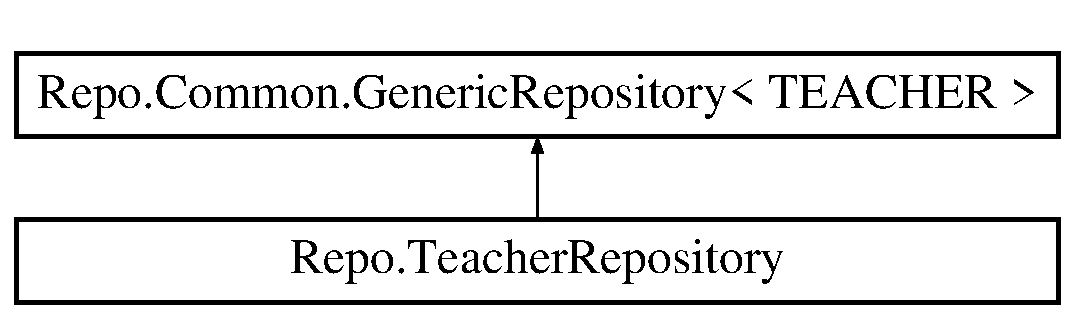
\includegraphics[height=2.000000cm]{class_repo_1_1_teacher_repository}
\end{center}
\end{figure}
\subsection*{Public Member Functions}
\begin{DoxyCompactItemize}
\item 
\hyperlink{class_repo_1_1_teacher_repository_a632e6bc926978d77645253d3ada1a350}{Teacher\+Repository} (Db\+Context context)
\end{DoxyCompactItemize}
\subsection*{Additional Inherited Members}


\subsection{Constructor \& Destructor Documentation}
\mbox{\Hypertarget{class_repo_1_1_teacher_repository_a632e6bc926978d77645253d3ada1a350}\label{class_repo_1_1_teacher_repository_a632e6bc926978d77645253d3ada1a350}} 
\index{Repo\+::\+Teacher\+Repository@{Repo\+::\+Teacher\+Repository}!Teacher\+Repository@{Teacher\+Repository}}
\index{Teacher\+Repository@{Teacher\+Repository}!Repo\+::\+Teacher\+Repository@{Repo\+::\+Teacher\+Repository}}
\subsubsection{\texorpdfstring{Teacher\+Repository()}{TeacherRepository()}}
{\footnotesize\ttfamily Repo.\+Teacher\+Repository.\+Teacher\+Repository (\begin{DoxyParamCaption}\item[{Db\+Context}]{context }\end{DoxyParamCaption})}



The documentation for this class was generated from the following file\+:\begin{DoxyCompactItemize}
\item 
D\+:/\+\_\+\+W\+O\+R\+K/\+\_\+\+S\+T\+E\+P/\+In\+Study\+Asp/\+Repo/\hyperlink{_teacher_repository_8cs}{Teacher\+Repository.\+cs}\end{DoxyCompactItemize}

\hypertarget{class_teacher_validator}{}\section{Teacher\+Validator Class Reference}
\label{class_teacher_validator}\index{Teacher\+Validator@{Teacher\+Validator}}


Teacher registration validator.  


Inheritance diagram for Teacher\+Validator\+:\begin{figure}[H]
\begin{center}
\leavevmode
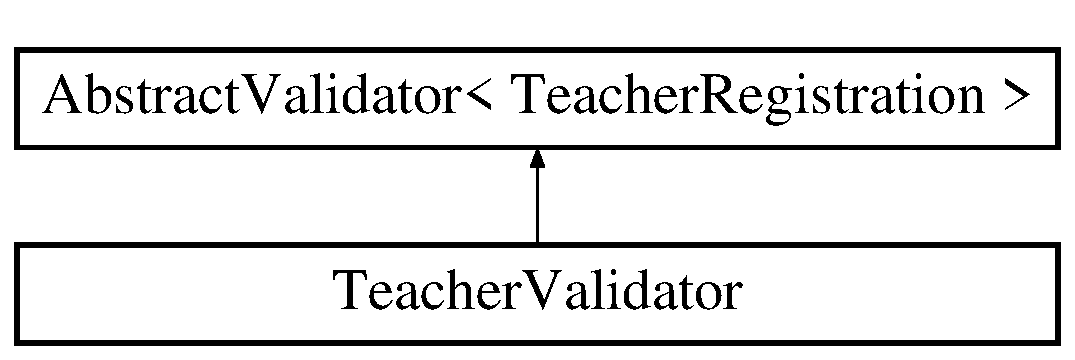
\includegraphics[height=2.000000cm]{class_teacher_validator}
\end{center}
\end{figure}
\subsection*{Public Member Functions}
\begin{DoxyCompactItemize}
\item 
\hyperlink{class_teacher_validator_a162804c2df0ecfa8d24679af271fad76}{Teacher\+Validator} ()
\end{DoxyCompactItemize}


\subsection{Detailed Description}
Teacher registration validator. 

\subsection{Constructor \& Destructor Documentation}
\mbox{\Hypertarget{class_teacher_validator_a162804c2df0ecfa8d24679af271fad76}\label{class_teacher_validator_a162804c2df0ecfa8d24679af271fad76}} 
\index{Teacher\+Validator@{Teacher\+Validator}!Teacher\+Validator@{Teacher\+Validator}}
\index{Teacher\+Validator@{Teacher\+Validator}!Teacher\+Validator@{Teacher\+Validator}}
\subsubsection{\texorpdfstring{Teacher\+Validator()}{TeacherValidator()}}
{\footnotesize\ttfamily Teacher\+Validator.\+Teacher\+Validator (\begin{DoxyParamCaption}{ }\end{DoxyParamCaption})}



The documentation for this class was generated from the following file\+:\begin{DoxyCompactItemize}
\item 
D\+:/\+\_\+\+W\+O\+R\+K/\+\_\+\+S\+T\+E\+P/\+In\+Study\+Asp/\+In\+Study\+Asp/\+Models/\+User/\+Teacher/\hyperlink{_teacher_registration_8cs}{Teacher\+Registration.\+cs}\end{DoxyCompactItemize}

\hypertarget{class_in_study_asp_1_1_controllers_1_1_user_1_1_student_1_1_test_student_controller}{}\section{In\+Study\+Asp.\+Controllers.\+User.\+Student.\+Test\+Student\+Controller Class Reference}
\label{class_in_study_asp_1_1_controllers_1_1_user_1_1_student_1_1_test_student_controller}\index{In\+Study\+Asp.\+Controllers.\+User.\+Student.\+Test\+Student\+Controller@{In\+Study\+Asp.\+Controllers.\+User.\+Student.\+Test\+Student\+Controller}}
Inheritance diagram for In\+Study\+Asp.\+Controllers.\+User.\+Student.\+Test\+Student\+Controller\+:\begin{figure}[H]
\begin{center}
\leavevmode
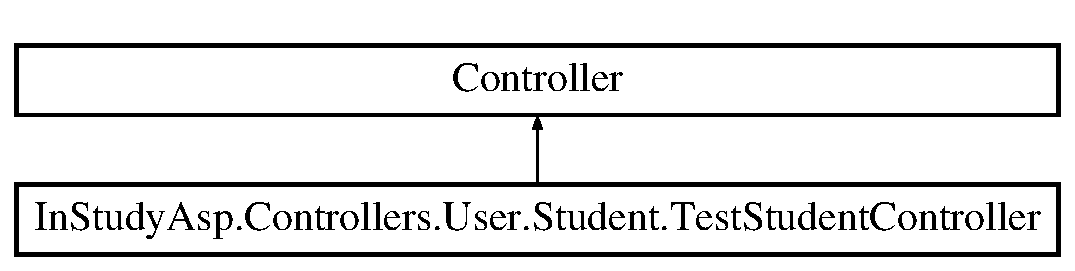
\includegraphics[height=2.000000cm]{class_in_study_asp_1_1_controllers_1_1_user_1_1_student_1_1_test_student_controller}
\end{center}
\end{figure}
\subsection*{Public Member Functions}
\begin{DoxyCompactItemize}
\item 
Action\+Result \hyperlink{class_in_study_asp_1_1_controllers_1_1_user_1_1_student_1_1_test_student_controller_a9bee94150395832ec87d244051a20130}{Index} ()
\end{DoxyCompactItemize}


\subsection{Member Function Documentation}
\mbox{\Hypertarget{class_in_study_asp_1_1_controllers_1_1_user_1_1_student_1_1_test_student_controller_a9bee94150395832ec87d244051a20130}\label{class_in_study_asp_1_1_controllers_1_1_user_1_1_student_1_1_test_student_controller_a9bee94150395832ec87d244051a20130}} 
\index{In\+Study\+Asp\+::\+Controllers\+::\+User\+::\+Student\+::\+Test\+Student\+Controller@{In\+Study\+Asp\+::\+Controllers\+::\+User\+::\+Student\+::\+Test\+Student\+Controller}!Index@{Index}}
\index{Index@{Index}!In\+Study\+Asp\+::\+Controllers\+::\+User\+::\+Student\+::\+Test\+Student\+Controller@{In\+Study\+Asp\+::\+Controllers\+::\+User\+::\+Student\+::\+Test\+Student\+Controller}}
\subsubsection{\texorpdfstring{Index()}{Index()}}
{\footnotesize\ttfamily Action\+Result In\+Study\+Asp.\+Controllers.\+User.\+Student.\+Test\+Student\+Controller.\+Index (\begin{DoxyParamCaption}{ }\end{DoxyParamCaption})}



The documentation for this class was generated from the following file\+:\begin{DoxyCompactItemize}
\item 
D\+:/\+\_\+\+W\+O\+R\+K/\+\_\+\+S\+T\+E\+P/\+In\+Study\+Asp/\+In\+Study\+Asp/\+Controllers/\+User/\+Student/\hyperlink{_test_student_controller_8cs}{Test\+Student\+Controller.\+cs}\end{DoxyCompactItemize}

\hypertarget{class_e_f_oracle_1_1_model_1_1_u_s_e_r}{}\section{E\+F\+Oracle.\+Model.\+U\+S\+ER Class Reference}
\label{class_e_f_oracle_1_1_model_1_1_u_s_e_r}\index{E\+F\+Oracle.\+Model.\+U\+S\+ER@{E\+F\+Oracle.\+Model.\+U\+S\+ER}}
\subsection*{Public Member Functions}
\begin{DoxyCompactItemize}
\item 
\hyperlink{class_e_f_oracle_1_1_model_1_1_u_s_e_r_a72a8423da1625bbd96ebf3e256e2e69d}{U\+S\+ER} ()
\end{DoxyCompactItemize}
\subsection*{Properties}
\begin{DoxyCompactItemize}
\item 
string \hyperlink{class_e_f_oracle_1_1_model_1_1_u_s_e_r_af17afbb891a92e46288022d64b7a8393}{U\+S\+E\+R\+\_\+\+P\+H\+O\+NE}\hspace{0.3cm}{\ttfamily  \mbox{[}get, set\mbox{]}}
\item 
string \hyperlink{class_e_f_oracle_1_1_model_1_1_u_s_e_r_a89dccb5c29dd3c072978fc465500c7af}{U\+S\+E\+R\+\_\+\+P\+A\+S\+S\+W\+O\+RD}\hspace{0.3cm}{\ttfamily  \mbox{[}get, set\mbox{]}}
\item 
string \hyperlink{class_e_f_oracle_1_1_model_1_1_u_s_e_r_a8f3418b6e13510654282c0079b2b52d5}{U\+S\+E\+R\+\_\+\+E\+M\+A\+IL}\hspace{0.3cm}{\ttfamily  \mbox{[}get, set\mbox{]}}
\item 
string \hyperlink{class_e_f_oracle_1_1_model_1_1_u_s_e_r_a92206079968e1447584054eb4da2be62}{U\+S\+E\+R\+\_\+\+F\+I\+R\+S\+T\+N\+A\+ME}\hspace{0.3cm}{\ttfamily  \mbox{[}get, set\mbox{]}}
\item 
string \hyperlink{class_e_f_oracle_1_1_model_1_1_u_s_e_r_a1521baf6b374d79498dc8d875190a772}{U\+S\+E\+R\+\_\+\+L\+A\+S\+T\+N\+A\+ME}\hspace{0.3cm}{\ttfamily  \mbox{[}get, set\mbox{]}}
\item 
Date\+Time \hyperlink{class_e_f_oracle_1_1_model_1_1_u_s_e_r_a20f6ec89e28a3aa3dfd8b934dce96368}{U\+S\+E\+R\+\_\+\+B\+I\+R\+T\+H\+D\+AY}\hspace{0.3cm}{\ttfamily  \mbox{[}get, set\mbox{]}}
\item 
byte \mbox{[}$\,$\mbox{]} \hyperlink{class_e_f_oracle_1_1_model_1_1_u_s_e_r_aada09caebf78d842b47abada413e5c90}{U\+S\+E\+R\+\_\+\+A\+V\+A\+T\+AR}\hspace{0.3cm}{\ttfamily  \mbox{[}get, set\mbox{]}}
\item 
decimal \hyperlink{class_e_f_oracle_1_1_model_1_1_u_s_e_r_a657bb6066915190f224c4fd7643ba413}{U\+S\+E\+R\+\_\+\+I\+S\+\_\+\+A\+C\+T\+I\+V\+A\+T\+ED}\hspace{0.3cm}{\ttfamily  \mbox{[}get, set\mbox{]}}
\item 
virtual I\+Collection$<$ \hyperlink{class_e_f_oracle_1_1_model_1_1_s_t_u_d_e_n_t}{S\+T\+U\+D\+E\+NT} $>$ \hyperlink{class_e_f_oracle_1_1_model_1_1_u_s_e_r_a4f9c5bb7b6fff133bd167b6f9e7ce81c}{S\+T\+U\+D\+E\+N\+Ts}\hspace{0.3cm}{\ttfamily  \mbox{[}get, set\mbox{]}}
\item 
virtual I\+Collection$<$ \hyperlink{class_e_f_oracle_1_1_model_1_1_t_e_a_c_h_e_r}{T\+E\+A\+C\+H\+ER} $>$ \hyperlink{class_e_f_oracle_1_1_model_1_1_u_s_e_r_a3326de9bfa91577cf2e251ed9d20ae7b}{T\+E\+A\+C\+H\+E\+Rs}\hspace{0.3cm}{\ttfamily  \mbox{[}get, set\mbox{]}}
\item 
virtual I\+Collection$<$ \hyperlink{class_e_f_oracle_1_1_model_1_1_u_s_e_r___s_e_s_s_i_o_n}{U\+S\+E\+R\+\_\+\+S\+E\+S\+S\+I\+ON} $>$ \hyperlink{class_e_f_oracle_1_1_model_1_1_u_s_e_r_aaffe4688e7551402b754435df6369ffe}{U\+S\+E\+R\+\_\+\+S\+E\+S\+S\+I\+ON}\hspace{0.3cm}{\ttfamily  \mbox{[}get, set\mbox{]}}
\end{DoxyCompactItemize}


\subsection{Constructor \& Destructor Documentation}
\mbox{\Hypertarget{class_e_f_oracle_1_1_model_1_1_u_s_e_r_a72a8423da1625bbd96ebf3e256e2e69d}\label{class_e_f_oracle_1_1_model_1_1_u_s_e_r_a72a8423da1625bbd96ebf3e256e2e69d}} 
\index{E\+F\+Oracle\+::\+Model\+::\+U\+S\+ER@{E\+F\+Oracle\+::\+Model\+::\+U\+S\+ER}!U\+S\+ER@{U\+S\+ER}}
\index{U\+S\+ER@{U\+S\+ER}!E\+F\+Oracle\+::\+Model\+::\+U\+S\+ER@{E\+F\+Oracle\+::\+Model\+::\+U\+S\+ER}}
\subsubsection{\texorpdfstring{U\+S\+E\+R()}{USER()}}
{\footnotesize\ttfamily E\+F\+Oracle.\+Model.\+U\+S\+E\+R.\+U\+S\+ER (\begin{DoxyParamCaption}{ }\end{DoxyParamCaption})}



\subsection{Property Documentation}
\mbox{\Hypertarget{class_e_f_oracle_1_1_model_1_1_u_s_e_r_a4f9c5bb7b6fff133bd167b6f9e7ce81c}\label{class_e_f_oracle_1_1_model_1_1_u_s_e_r_a4f9c5bb7b6fff133bd167b6f9e7ce81c}} 
\index{E\+F\+Oracle\+::\+Model\+::\+U\+S\+ER@{E\+F\+Oracle\+::\+Model\+::\+U\+S\+ER}!S\+T\+U\+D\+E\+N\+Ts@{S\+T\+U\+D\+E\+N\+Ts}}
\index{S\+T\+U\+D\+E\+N\+Ts@{S\+T\+U\+D\+E\+N\+Ts}!E\+F\+Oracle\+::\+Model\+::\+U\+S\+ER@{E\+F\+Oracle\+::\+Model\+::\+U\+S\+ER}}
\subsubsection{\texorpdfstring{S\+T\+U\+D\+E\+N\+Ts}{STUDENTs}}
{\footnotesize\ttfamily virtual I\+Collection$<$\hyperlink{class_e_f_oracle_1_1_model_1_1_s_t_u_d_e_n_t}{S\+T\+U\+D\+E\+NT}$>$ E\+F\+Oracle.\+Model.\+U\+S\+E\+R.\+S\+T\+U\+D\+E\+N\+Ts\hspace{0.3cm}{\ttfamily [get]}, {\ttfamily [set]}}

\mbox{\Hypertarget{class_e_f_oracle_1_1_model_1_1_u_s_e_r_a3326de9bfa91577cf2e251ed9d20ae7b}\label{class_e_f_oracle_1_1_model_1_1_u_s_e_r_a3326de9bfa91577cf2e251ed9d20ae7b}} 
\index{E\+F\+Oracle\+::\+Model\+::\+U\+S\+ER@{E\+F\+Oracle\+::\+Model\+::\+U\+S\+ER}!T\+E\+A\+C\+H\+E\+Rs@{T\+E\+A\+C\+H\+E\+Rs}}
\index{T\+E\+A\+C\+H\+E\+Rs@{T\+E\+A\+C\+H\+E\+Rs}!E\+F\+Oracle\+::\+Model\+::\+U\+S\+ER@{E\+F\+Oracle\+::\+Model\+::\+U\+S\+ER}}
\subsubsection{\texorpdfstring{T\+E\+A\+C\+H\+E\+Rs}{TEACHERs}}
{\footnotesize\ttfamily virtual I\+Collection$<$\hyperlink{class_e_f_oracle_1_1_model_1_1_t_e_a_c_h_e_r}{T\+E\+A\+C\+H\+ER}$>$ E\+F\+Oracle.\+Model.\+U\+S\+E\+R.\+T\+E\+A\+C\+H\+E\+Rs\hspace{0.3cm}{\ttfamily [get]}, {\ttfamily [set]}}

\mbox{\Hypertarget{class_e_f_oracle_1_1_model_1_1_u_s_e_r_aada09caebf78d842b47abada413e5c90}\label{class_e_f_oracle_1_1_model_1_1_u_s_e_r_aada09caebf78d842b47abada413e5c90}} 
\index{E\+F\+Oracle\+::\+Model\+::\+U\+S\+ER@{E\+F\+Oracle\+::\+Model\+::\+U\+S\+ER}!U\+S\+E\+R\+\_\+\+A\+V\+A\+T\+AR@{U\+S\+E\+R\+\_\+\+A\+V\+A\+T\+AR}}
\index{U\+S\+E\+R\+\_\+\+A\+V\+A\+T\+AR@{U\+S\+E\+R\+\_\+\+A\+V\+A\+T\+AR}!E\+F\+Oracle\+::\+Model\+::\+U\+S\+ER@{E\+F\+Oracle\+::\+Model\+::\+U\+S\+ER}}
\subsubsection{\texorpdfstring{U\+S\+E\+R\+\_\+\+A\+V\+A\+T\+AR}{USER\_AVATAR}}
{\footnotesize\ttfamily byte \mbox{[}$\,$\mbox{]} E\+F\+Oracle.\+Model.\+U\+S\+E\+R.\+U\+S\+E\+R\+\_\+\+A\+V\+A\+T\+AR\hspace{0.3cm}{\ttfamily [get]}, {\ttfamily [set]}}

\mbox{\Hypertarget{class_e_f_oracle_1_1_model_1_1_u_s_e_r_a20f6ec89e28a3aa3dfd8b934dce96368}\label{class_e_f_oracle_1_1_model_1_1_u_s_e_r_a20f6ec89e28a3aa3dfd8b934dce96368}} 
\index{E\+F\+Oracle\+::\+Model\+::\+U\+S\+ER@{E\+F\+Oracle\+::\+Model\+::\+U\+S\+ER}!U\+S\+E\+R\+\_\+\+B\+I\+R\+T\+H\+D\+AY@{U\+S\+E\+R\+\_\+\+B\+I\+R\+T\+H\+D\+AY}}
\index{U\+S\+E\+R\+\_\+\+B\+I\+R\+T\+H\+D\+AY@{U\+S\+E\+R\+\_\+\+B\+I\+R\+T\+H\+D\+AY}!E\+F\+Oracle\+::\+Model\+::\+U\+S\+ER@{E\+F\+Oracle\+::\+Model\+::\+U\+S\+ER}}
\subsubsection{\texorpdfstring{U\+S\+E\+R\+\_\+\+B\+I\+R\+T\+H\+D\+AY}{USER\_BIRTHDAY}}
{\footnotesize\ttfamily Date\+Time E\+F\+Oracle.\+Model.\+U\+S\+E\+R.\+U\+S\+E\+R\+\_\+\+B\+I\+R\+T\+H\+D\+AY\hspace{0.3cm}{\ttfamily [get]}, {\ttfamily [set]}}

\mbox{\Hypertarget{class_e_f_oracle_1_1_model_1_1_u_s_e_r_a8f3418b6e13510654282c0079b2b52d5}\label{class_e_f_oracle_1_1_model_1_1_u_s_e_r_a8f3418b6e13510654282c0079b2b52d5}} 
\index{E\+F\+Oracle\+::\+Model\+::\+U\+S\+ER@{E\+F\+Oracle\+::\+Model\+::\+U\+S\+ER}!U\+S\+E\+R\+\_\+\+E\+M\+A\+IL@{U\+S\+E\+R\+\_\+\+E\+M\+A\+IL}}
\index{U\+S\+E\+R\+\_\+\+E\+M\+A\+IL@{U\+S\+E\+R\+\_\+\+E\+M\+A\+IL}!E\+F\+Oracle\+::\+Model\+::\+U\+S\+ER@{E\+F\+Oracle\+::\+Model\+::\+U\+S\+ER}}
\subsubsection{\texorpdfstring{U\+S\+E\+R\+\_\+\+E\+M\+A\+IL}{USER\_EMAIL}}
{\footnotesize\ttfamily string E\+F\+Oracle.\+Model.\+U\+S\+E\+R.\+U\+S\+E\+R\+\_\+\+E\+M\+A\+IL\hspace{0.3cm}{\ttfamily [get]}, {\ttfamily [set]}}

\mbox{\Hypertarget{class_e_f_oracle_1_1_model_1_1_u_s_e_r_a92206079968e1447584054eb4da2be62}\label{class_e_f_oracle_1_1_model_1_1_u_s_e_r_a92206079968e1447584054eb4da2be62}} 
\index{E\+F\+Oracle\+::\+Model\+::\+U\+S\+ER@{E\+F\+Oracle\+::\+Model\+::\+U\+S\+ER}!U\+S\+E\+R\+\_\+\+F\+I\+R\+S\+T\+N\+A\+ME@{U\+S\+E\+R\+\_\+\+F\+I\+R\+S\+T\+N\+A\+ME}}
\index{U\+S\+E\+R\+\_\+\+F\+I\+R\+S\+T\+N\+A\+ME@{U\+S\+E\+R\+\_\+\+F\+I\+R\+S\+T\+N\+A\+ME}!E\+F\+Oracle\+::\+Model\+::\+U\+S\+ER@{E\+F\+Oracle\+::\+Model\+::\+U\+S\+ER}}
\subsubsection{\texorpdfstring{U\+S\+E\+R\+\_\+\+F\+I\+R\+S\+T\+N\+A\+ME}{USER\_FIRSTNAME}}
{\footnotesize\ttfamily string E\+F\+Oracle.\+Model.\+U\+S\+E\+R.\+U\+S\+E\+R\+\_\+\+F\+I\+R\+S\+T\+N\+A\+ME\hspace{0.3cm}{\ttfamily [get]}, {\ttfamily [set]}}

\mbox{\Hypertarget{class_e_f_oracle_1_1_model_1_1_u_s_e_r_a657bb6066915190f224c4fd7643ba413}\label{class_e_f_oracle_1_1_model_1_1_u_s_e_r_a657bb6066915190f224c4fd7643ba413}} 
\index{E\+F\+Oracle\+::\+Model\+::\+U\+S\+ER@{E\+F\+Oracle\+::\+Model\+::\+U\+S\+ER}!U\+S\+E\+R\+\_\+\+I\+S\+\_\+\+A\+C\+T\+I\+V\+A\+T\+ED@{U\+S\+E\+R\+\_\+\+I\+S\+\_\+\+A\+C\+T\+I\+V\+A\+T\+ED}}
\index{U\+S\+E\+R\+\_\+\+I\+S\+\_\+\+A\+C\+T\+I\+V\+A\+T\+ED@{U\+S\+E\+R\+\_\+\+I\+S\+\_\+\+A\+C\+T\+I\+V\+A\+T\+ED}!E\+F\+Oracle\+::\+Model\+::\+U\+S\+ER@{E\+F\+Oracle\+::\+Model\+::\+U\+S\+ER}}
\subsubsection{\texorpdfstring{U\+S\+E\+R\+\_\+\+I\+S\+\_\+\+A\+C\+T\+I\+V\+A\+T\+ED}{USER\_IS\_ACTIVATED}}
{\footnotesize\ttfamily decimal E\+F\+Oracle.\+Model.\+U\+S\+E\+R.\+U\+S\+E\+R\+\_\+\+I\+S\+\_\+\+A\+C\+T\+I\+V\+A\+T\+ED\hspace{0.3cm}{\ttfamily [get]}, {\ttfamily [set]}}

\mbox{\Hypertarget{class_e_f_oracle_1_1_model_1_1_u_s_e_r_a1521baf6b374d79498dc8d875190a772}\label{class_e_f_oracle_1_1_model_1_1_u_s_e_r_a1521baf6b374d79498dc8d875190a772}} 
\index{E\+F\+Oracle\+::\+Model\+::\+U\+S\+ER@{E\+F\+Oracle\+::\+Model\+::\+U\+S\+ER}!U\+S\+E\+R\+\_\+\+L\+A\+S\+T\+N\+A\+ME@{U\+S\+E\+R\+\_\+\+L\+A\+S\+T\+N\+A\+ME}}
\index{U\+S\+E\+R\+\_\+\+L\+A\+S\+T\+N\+A\+ME@{U\+S\+E\+R\+\_\+\+L\+A\+S\+T\+N\+A\+ME}!E\+F\+Oracle\+::\+Model\+::\+U\+S\+ER@{E\+F\+Oracle\+::\+Model\+::\+U\+S\+ER}}
\subsubsection{\texorpdfstring{U\+S\+E\+R\+\_\+\+L\+A\+S\+T\+N\+A\+ME}{USER\_LASTNAME}}
{\footnotesize\ttfamily string E\+F\+Oracle.\+Model.\+U\+S\+E\+R.\+U\+S\+E\+R\+\_\+\+L\+A\+S\+T\+N\+A\+ME\hspace{0.3cm}{\ttfamily [get]}, {\ttfamily [set]}}

\mbox{\Hypertarget{class_e_f_oracle_1_1_model_1_1_u_s_e_r_a89dccb5c29dd3c072978fc465500c7af}\label{class_e_f_oracle_1_1_model_1_1_u_s_e_r_a89dccb5c29dd3c072978fc465500c7af}} 
\index{E\+F\+Oracle\+::\+Model\+::\+U\+S\+ER@{E\+F\+Oracle\+::\+Model\+::\+U\+S\+ER}!U\+S\+E\+R\+\_\+\+P\+A\+S\+S\+W\+O\+RD@{U\+S\+E\+R\+\_\+\+P\+A\+S\+S\+W\+O\+RD}}
\index{U\+S\+E\+R\+\_\+\+P\+A\+S\+S\+W\+O\+RD@{U\+S\+E\+R\+\_\+\+P\+A\+S\+S\+W\+O\+RD}!E\+F\+Oracle\+::\+Model\+::\+U\+S\+ER@{E\+F\+Oracle\+::\+Model\+::\+U\+S\+ER}}
\subsubsection{\texorpdfstring{U\+S\+E\+R\+\_\+\+P\+A\+S\+S\+W\+O\+RD}{USER\_PASSWORD}}
{\footnotesize\ttfamily string E\+F\+Oracle.\+Model.\+U\+S\+E\+R.\+U\+S\+E\+R\+\_\+\+P\+A\+S\+S\+W\+O\+RD\hspace{0.3cm}{\ttfamily [get]}, {\ttfamily [set]}}

\mbox{\Hypertarget{class_e_f_oracle_1_1_model_1_1_u_s_e_r_af17afbb891a92e46288022d64b7a8393}\label{class_e_f_oracle_1_1_model_1_1_u_s_e_r_af17afbb891a92e46288022d64b7a8393}} 
\index{E\+F\+Oracle\+::\+Model\+::\+U\+S\+ER@{E\+F\+Oracle\+::\+Model\+::\+U\+S\+ER}!U\+S\+E\+R\+\_\+\+P\+H\+O\+NE@{U\+S\+E\+R\+\_\+\+P\+H\+O\+NE}}
\index{U\+S\+E\+R\+\_\+\+P\+H\+O\+NE@{U\+S\+E\+R\+\_\+\+P\+H\+O\+NE}!E\+F\+Oracle\+::\+Model\+::\+U\+S\+ER@{E\+F\+Oracle\+::\+Model\+::\+U\+S\+ER}}
\subsubsection{\texorpdfstring{U\+S\+E\+R\+\_\+\+P\+H\+O\+NE}{USER\_PHONE}}
{\footnotesize\ttfamily string E\+F\+Oracle.\+Model.\+U\+S\+E\+R.\+U\+S\+E\+R\+\_\+\+P\+H\+O\+NE\hspace{0.3cm}{\ttfamily [get]}, {\ttfamily [set]}}

\mbox{\Hypertarget{class_e_f_oracle_1_1_model_1_1_u_s_e_r_aaffe4688e7551402b754435df6369ffe}\label{class_e_f_oracle_1_1_model_1_1_u_s_e_r_aaffe4688e7551402b754435df6369ffe}} 
\index{E\+F\+Oracle\+::\+Model\+::\+U\+S\+ER@{E\+F\+Oracle\+::\+Model\+::\+U\+S\+ER}!U\+S\+E\+R\+\_\+\+S\+E\+S\+S\+I\+ON@{U\+S\+E\+R\+\_\+\+S\+E\+S\+S\+I\+ON}}
\index{U\+S\+E\+R\+\_\+\+S\+E\+S\+S\+I\+ON@{U\+S\+E\+R\+\_\+\+S\+E\+S\+S\+I\+ON}!E\+F\+Oracle\+::\+Model\+::\+U\+S\+ER@{E\+F\+Oracle\+::\+Model\+::\+U\+S\+ER}}
\subsubsection{\texorpdfstring{U\+S\+E\+R\+\_\+\+S\+E\+S\+S\+I\+ON}{USER\_SESSION}}
{\footnotesize\ttfamily virtual I\+Collection$<$\hyperlink{class_e_f_oracle_1_1_model_1_1_u_s_e_r___s_e_s_s_i_o_n}{U\+S\+E\+R\+\_\+\+S\+E\+S\+S\+I\+ON}$>$ E\+F\+Oracle.\+Model.\+U\+S\+E\+R.\+U\+S\+E\+R\+\_\+\+S\+E\+S\+S\+I\+ON\hspace{0.3cm}{\ttfamily [get]}, {\ttfamily [set]}}



The documentation for this class was generated from the following file\+:\begin{DoxyCompactItemize}
\item 
D\+:/\+\_\+\+W\+O\+R\+K/\+\_\+\+S\+T\+E\+P/\+In\+Study\+Asp/\+E\+F\+Oracle/\+Model/\hyperlink{_u_s_e_r_8cs}{U\+S\+E\+R.\+cs}\end{DoxyCompactItemize}

\hypertarget{class_e_f_oracle_1_1_model_1_1_u_s_e_r___s_e_s_s_i_o_n}{}\section{E\+F\+Oracle.\+Model.\+U\+S\+E\+R\+\_\+\+S\+E\+S\+S\+I\+ON Class Reference}
\label{class_e_f_oracle_1_1_model_1_1_u_s_e_r___s_e_s_s_i_o_n}\index{E\+F\+Oracle.\+Model.\+U\+S\+E\+R\+\_\+\+S\+E\+S\+S\+I\+ON@{E\+F\+Oracle.\+Model.\+U\+S\+E\+R\+\_\+\+S\+E\+S\+S\+I\+ON}}
\subsection*{Properties}
\begin{DoxyCompactItemize}
\item 
string \hyperlink{class_e_f_oracle_1_1_model_1_1_u_s_e_r___s_e_s_s_i_o_n_a68959ea6dd53308cc7f49027d86d4fd2}{U\+S\+E\+R\+\_\+\+P\+H\+O\+N\+E\+\_\+\+FK}\hspace{0.3cm}{\ttfamily  \mbox{[}get, set\mbox{]}}
\item 
Date\+Time \hyperlink{class_e_f_oracle_1_1_model_1_1_u_s_e_r___s_e_s_s_i_o_n_a234044b2c332bf682dbdf1f58179a493}{S\+E\+S\+S\+I\+O\+N\+\_\+\+D\+A\+T\+E\+T\+I\+ME}\hspace{0.3cm}{\ttfamily  \mbox{[}get, set\mbox{]}}
\item 
string \hyperlink{class_e_f_oracle_1_1_model_1_1_u_s_e_r___s_e_s_s_i_o_n_ac59ad604d706879163681a09421eea95}{S\+E\+S\+S\+I\+O\+N\+\_\+\+H\+A\+SH}\hspace{0.3cm}{\ttfamily  \mbox{[}get, set\mbox{]}}
\item 
Date\+Time \hyperlink{class_e_f_oracle_1_1_model_1_1_u_s_e_r___s_e_s_s_i_o_n_a5a7becbb18a66d1c457335e36ee7fd94}{S\+E\+S\+S\+I\+O\+N\+\_\+\+E\+X\+P\+I\+RE}\hspace{0.3cm}{\ttfamily  \mbox{[}get, set\mbox{]}}
\item 
virtual \hyperlink{class_e_f_oracle_1_1_model_1_1_u_s_e_r}{U\+S\+ER} \hyperlink{class_e_f_oracle_1_1_model_1_1_u_s_e_r___s_e_s_s_i_o_n_acf0791e197b026b18713de020c3ce7e1}{U\+S\+ER}\hspace{0.3cm}{\ttfamily  \mbox{[}get, set\mbox{]}}
\end{DoxyCompactItemize}


\subsection{Property Documentation}
\mbox{\Hypertarget{class_e_f_oracle_1_1_model_1_1_u_s_e_r___s_e_s_s_i_o_n_a234044b2c332bf682dbdf1f58179a493}\label{class_e_f_oracle_1_1_model_1_1_u_s_e_r___s_e_s_s_i_o_n_a234044b2c332bf682dbdf1f58179a493}} 
\index{E\+F\+Oracle\+::\+Model\+::\+U\+S\+E\+R\+\_\+\+S\+E\+S\+S\+I\+ON@{E\+F\+Oracle\+::\+Model\+::\+U\+S\+E\+R\+\_\+\+S\+E\+S\+S\+I\+ON}!S\+E\+S\+S\+I\+O\+N\+\_\+\+D\+A\+T\+E\+T\+I\+ME@{S\+E\+S\+S\+I\+O\+N\+\_\+\+D\+A\+T\+E\+T\+I\+ME}}
\index{S\+E\+S\+S\+I\+O\+N\+\_\+\+D\+A\+T\+E\+T\+I\+ME@{S\+E\+S\+S\+I\+O\+N\+\_\+\+D\+A\+T\+E\+T\+I\+ME}!E\+F\+Oracle\+::\+Model\+::\+U\+S\+E\+R\+\_\+\+S\+E\+S\+S\+I\+ON@{E\+F\+Oracle\+::\+Model\+::\+U\+S\+E\+R\+\_\+\+S\+E\+S\+S\+I\+ON}}
\subsubsection{\texorpdfstring{S\+E\+S\+S\+I\+O\+N\+\_\+\+D\+A\+T\+E\+T\+I\+ME}{SESSION\_DATETIME}}
{\footnotesize\ttfamily Date\+Time E\+F\+Oracle.\+Model.\+U\+S\+E\+R\+\_\+\+S\+E\+S\+S\+I\+O\+N.\+S\+E\+S\+S\+I\+O\+N\+\_\+\+D\+A\+T\+E\+T\+I\+ME\hspace{0.3cm}{\ttfamily [get]}, {\ttfamily [set]}}

\mbox{\Hypertarget{class_e_f_oracle_1_1_model_1_1_u_s_e_r___s_e_s_s_i_o_n_a5a7becbb18a66d1c457335e36ee7fd94}\label{class_e_f_oracle_1_1_model_1_1_u_s_e_r___s_e_s_s_i_o_n_a5a7becbb18a66d1c457335e36ee7fd94}} 
\index{E\+F\+Oracle\+::\+Model\+::\+U\+S\+E\+R\+\_\+\+S\+E\+S\+S\+I\+ON@{E\+F\+Oracle\+::\+Model\+::\+U\+S\+E\+R\+\_\+\+S\+E\+S\+S\+I\+ON}!S\+E\+S\+S\+I\+O\+N\+\_\+\+E\+X\+P\+I\+RE@{S\+E\+S\+S\+I\+O\+N\+\_\+\+E\+X\+P\+I\+RE}}
\index{S\+E\+S\+S\+I\+O\+N\+\_\+\+E\+X\+P\+I\+RE@{S\+E\+S\+S\+I\+O\+N\+\_\+\+E\+X\+P\+I\+RE}!E\+F\+Oracle\+::\+Model\+::\+U\+S\+E\+R\+\_\+\+S\+E\+S\+S\+I\+ON@{E\+F\+Oracle\+::\+Model\+::\+U\+S\+E\+R\+\_\+\+S\+E\+S\+S\+I\+ON}}
\subsubsection{\texorpdfstring{S\+E\+S\+S\+I\+O\+N\+\_\+\+E\+X\+P\+I\+RE}{SESSION\_EXPIRE}}
{\footnotesize\ttfamily Date\+Time E\+F\+Oracle.\+Model.\+U\+S\+E\+R\+\_\+\+S\+E\+S\+S\+I\+O\+N.\+S\+E\+S\+S\+I\+O\+N\+\_\+\+E\+X\+P\+I\+RE\hspace{0.3cm}{\ttfamily [get]}, {\ttfamily [set]}}

\mbox{\Hypertarget{class_e_f_oracle_1_1_model_1_1_u_s_e_r___s_e_s_s_i_o_n_ac59ad604d706879163681a09421eea95}\label{class_e_f_oracle_1_1_model_1_1_u_s_e_r___s_e_s_s_i_o_n_ac59ad604d706879163681a09421eea95}} 
\index{E\+F\+Oracle\+::\+Model\+::\+U\+S\+E\+R\+\_\+\+S\+E\+S\+S\+I\+ON@{E\+F\+Oracle\+::\+Model\+::\+U\+S\+E\+R\+\_\+\+S\+E\+S\+S\+I\+ON}!S\+E\+S\+S\+I\+O\+N\+\_\+\+H\+A\+SH@{S\+E\+S\+S\+I\+O\+N\+\_\+\+H\+A\+SH}}
\index{S\+E\+S\+S\+I\+O\+N\+\_\+\+H\+A\+SH@{S\+E\+S\+S\+I\+O\+N\+\_\+\+H\+A\+SH}!E\+F\+Oracle\+::\+Model\+::\+U\+S\+E\+R\+\_\+\+S\+E\+S\+S\+I\+ON@{E\+F\+Oracle\+::\+Model\+::\+U\+S\+E\+R\+\_\+\+S\+E\+S\+S\+I\+ON}}
\subsubsection{\texorpdfstring{S\+E\+S\+S\+I\+O\+N\+\_\+\+H\+A\+SH}{SESSION\_HASH}}
{\footnotesize\ttfamily string E\+F\+Oracle.\+Model.\+U\+S\+E\+R\+\_\+\+S\+E\+S\+S\+I\+O\+N.\+S\+E\+S\+S\+I\+O\+N\+\_\+\+H\+A\+SH\hspace{0.3cm}{\ttfamily [get]}, {\ttfamily [set]}}

\mbox{\Hypertarget{class_e_f_oracle_1_1_model_1_1_u_s_e_r___s_e_s_s_i_o_n_acf0791e197b026b18713de020c3ce7e1}\label{class_e_f_oracle_1_1_model_1_1_u_s_e_r___s_e_s_s_i_o_n_acf0791e197b026b18713de020c3ce7e1}} 
\index{E\+F\+Oracle\+::\+Model\+::\+U\+S\+E\+R\+\_\+\+S\+E\+S\+S\+I\+ON@{E\+F\+Oracle\+::\+Model\+::\+U\+S\+E\+R\+\_\+\+S\+E\+S\+S\+I\+ON}!U\+S\+ER@{U\+S\+ER}}
\index{U\+S\+ER@{U\+S\+ER}!E\+F\+Oracle\+::\+Model\+::\+U\+S\+E\+R\+\_\+\+S\+E\+S\+S\+I\+ON@{E\+F\+Oracle\+::\+Model\+::\+U\+S\+E\+R\+\_\+\+S\+E\+S\+S\+I\+ON}}
\subsubsection{\texorpdfstring{U\+S\+ER}{USER}}
{\footnotesize\ttfamily virtual \hyperlink{class_e_f_oracle_1_1_model_1_1_u_s_e_r}{U\+S\+ER} E\+F\+Oracle.\+Model.\+U\+S\+E\+R\+\_\+\+S\+E\+S\+S\+I\+O\+N.\+U\+S\+ER\hspace{0.3cm}{\ttfamily [get]}, {\ttfamily [set]}}

\mbox{\Hypertarget{class_e_f_oracle_1_1_model_1_1_u_s_e_r___s_e_s_s_i_o_n_a68959ea6dd53308cc7f49027d86d4fd2}\label{class_e_f_oracle_1_1_model_1_1_u_s_e_r___s_e_s_s_i_o_n_a68959ea6dd53308cc7f49027d86d4fd2}} 
\index{E\+F\+Oracle\+::\+Model\+::\+U\+S\+E\+R\+\_\+\+S\+E\+S\+S\+I\+ON@{E\+F\+Oracle\+::\+Model\+::\+U\+S\+E\+R\+\_\+\+S\+E\+S\+S\+I\+ON}!U\+S\+E\+R\+\_\+\+P\+H\+O\+N\+E\+\_\+\+FK@{U\+S\+E\+R\+\_\+\+P\+H\+O\+N\+E\+\_\+\+FK}}
\index{U\+S\+E\+R\+\_\+\+P\+H\+O\+N\+E\+\_\+\+FK@{U\+S\+E\+R\+\_\+\+P\+H\+O\+N\+E\+\_\+\+FK}!E\+F\+Oracle\+::\+Model\+::\+U\+S\+E\+R\+\_\+\+S\+E\+S\+S\+I\+ON@{E\+F\+Oracle\+::\+Model\+::\+U\+S\+E\+R\+\_\+\+S\+E\+S\+S\+I\+ON}}
\subsubsection{\texorpdfstring{U\+S\+E\+R\+\_\+\+P\+H\+O\+N\+E\+\_\+\+FK}{USER\_PHONE\_FK}}
{\footnotesize\ttfamily string E\+F\+Oracle.\+Model.\+U\+S\+E\+R\+\_\+\+S\+E\+S\+S\+I\+O\+N.\+U\+S\+E\+R\+\_\+\+P\+H\+O\+N\+E\+\_\+\+FK\hspace{0.3cm}{\ttfamily [get]}, {\ttfamily [set]}}



The documentation for this class was generated from the following file\+:\begin{DoxyCompactItemize}
\item 
D\+:/\+\_\+\+W\+O\+R\+K/\+\_\+\+S\+T\+E\+P/\+In\+Study\+Asp/\+E\+F\+Oracle/\+Model/\hyperlink{_u_s_e_r___s_e_s_s_i_o_n_8cs}{U\+S\+E\+R\+\_\+\+S\+E\+S\+S\+I\+O\+N.\+cs}\end{DoxyCompactItemize}

\hypertarget{class_repo_1_1_user_repository}{}\section{Repo.\+User\+Repository Class Reference}
\label{class_repo_1_1_user_repository}\index{Repo.\+User\+Repository@{Repo.\+User\+Repository}}
Inheritance diagram for Repo.\+User\+Repository\+:\begin{figure}[H]
\begin{center}
\leavevmode
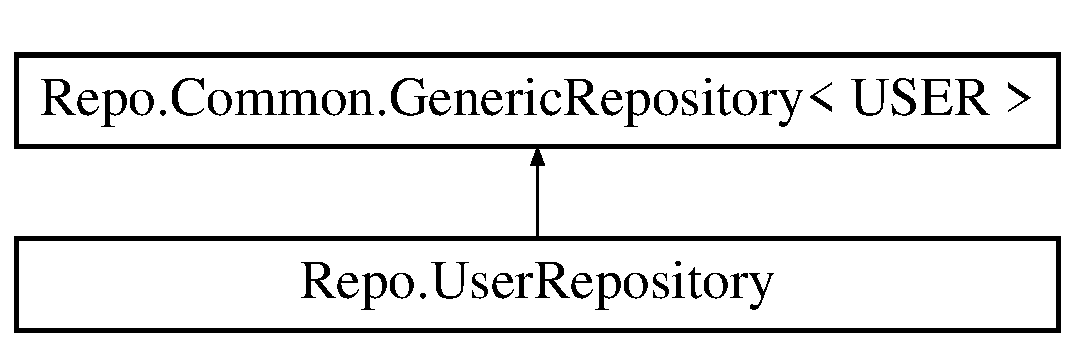
\includegraphics[height=2.000000cm]{class_repo_1_1_user_repository}
\end{center}
\end{figure}
\subsection*{Public Member Functions}
\begin{DoxyCompactItemize}
\item 
\hyperlink{class_repo_1_1_user_repository_ae1b1d6c1aa7578a0a280f4b457f5ffdf}{User\+Repository} (Db\+Context context)
\end{DoxyCompactItemize}
\subsection*{Additional Inherited Members}


\subsection{Constructor \& Destructor Documentation}
\mbox{\Hypertarget{class_repo_1_1_user_repository_ae1b1d6c1aa7578a0a280f4b457f5ffdf}\label{class_repo_1_1_user_repository_ae1b1d6c1aa7578a0a280f4b457f5ffdf}} 
\index{Repo\+::\+User\+Repository@{Repo\+::\+User\+Repository}!User\+Repository@{User\+Repository}}
\index{User\+Repository@{User\+Repository}!Repo\+::\+User\+Repository@{Repo\+::\+User\+Repository}}
\subsubsection{\texorpdfstring{User\+Repository()}{UserRepository()}}
{\footnotesize\ttfamily Repo.\+User\+Repository.\+User\+Repository (\begin{DoxyParamCaption}\item[{Db\+Context}]{context }\end{DoxyParamCaption})}



The documentation for this class was generated from the following file\+:\begin{DoxyCompactItemize}
\item 
D\+:/\+\_\+\+W\+O\+R\+K/\+\_\+\+S\+T\+E\+P/\+In\+Study\+Asp/\+Repo/\hyperlink{_user_repository_8cs}{User\+Repository.\+cs}\end{DoxyCompactItemize}

\hypertarget{class_in_study_asp_1_1_models_1_1_user_1_1_teacher_1_1_verification_mail_sender}{}\section{In\+Study\+Asp.\+Models.\+User.\+Teacher.\+Verification\+Mail\+Sender Class Reference}
\label{class_in_study_asp_1_1_models_1_1_user_1_1_teacher_1_1_verification_mail_sender}\index{In\+Study\+Asp.\+Models.\+User.\+Teacher.\+Verification\+Mail\+Sender@{In\+Study\+Asp.\+Models.\+User.\+Teacher.\+Verification\+Mail\+Sender}}


Mail sender.  


\subsection*{Public Member Functions}
\begin{DoxyCompactItemize}
\item 
void \hyperlink{class_in_study_asp_1_1_models_1_1_user_1_1_teacher_1_1_verification_mail_sender_a821243536c59c40a3a4ca9fb14a01597}{Send\+Verification\+Link\+Email} ()
\begin{DoxyCompactList}\small\item\em Sending mail method. \end{DoxyCompactList}\end{DoxyCompactItemize}
\subsection*{Properties}
\begin{DoxyCompactItemize}
\item 
Mail\+Address \hyperlink{class_in_study_asp_1_1_models_1_1_user_1_1_teacher_1_1_verification_mail_sender_a96fe95e9c2b44d798c6e80dc1c48644f}{From\+Email}\hspace{0.3cm}{\ttfamily  \mbox{[}get, set\mbox{]}}
\item 
Mail\+Address \hyperlink{class_in_study_asp_1_1_models_1_1_user_1_1_teacher_1_1_verification_mail_sender_a5d1a4989afd78fe89bbd9e16384f1ea0}{To\+Email}\hspace{0.3cm}{\ttfamily  \mbox{[}get, set\mbox{]}}
\item 
string \hyperlink{class_in_study_asp_1_1_models_1_1_user_1_1_teacher_1_1_verification_mail_sender_a2d722add9dc18d73f603f73117123187}{From\+Email\+Password}\hspace{0.3cm}{\ttfamily  \mbox{[}get, set\mbox{]}}
\item 
string \hyperlink{class_in_study_asp_1_1_models_1_1_user_1_1_teacher_1_1_verification_mail_sender_a216b4f2752660b4a6ecec2c773233d0c}{Subject}\hspace{0.3cm}{\ttfamily  \mbox{[}get, set\mbox{]}}
\item 
string \hyperlink{class_in_study_asp_1_1_models_1_1_user_1_1_teacher_1_1_verification_mail_sender_aa49b9314599d95938d0cd26308c505e5}{Body}\hspace{0.3cm}{\ttfamily  \mbox{[}get, set\mbox{]}}
\item 
string \hyperlink{class_in_study_asp_1_1_models_1_1_user_1_1_teacher_1_1_verification_mail_sender_afcf3bf429d484fd0e0de3d6042ee1b2c}{Link}\hspace{0.3cm}{\ttfamily  \mbox{[}get, set\mbox{]}}
\item 
string \hyperlink{class_in_study_asp_1_1_models_1_1_user_1_1_teacher_1_1_verification_mail_sender_a3f2bff52cb4ffcaee3cff7f40567a7aa}{Smtp\+Host}\hspace{0.3cm}{\ttfamily  \mbox{[}get, set\mbox{]}}
\item 
int \hyperlink{class_in_study_asp_1_1_models_1_1_user_1_1_teacher_1_1_verification_mail_sender_a010bef0a137e2b2cca0b0f3168e21849}{Smtp\+Port}\hspace{0.3cm}{\ttfamily  \mbox{[}get, set\mbox{]}}
\end{DoxyCompactItemize}


\subsection{Detailed Description}
Mail sender. 

\subsection{Member Function Documentation}
\mbox{\Hypertarget{class_in_study_asp_1_1_models_1_1_user_1_1_teacher_1_1_verification_mail_sender_a821243536c59c40a3a4ca9fb14a01597}\label{class_in_study_asp_1_1_models_1_1_user_1_1_teacher_1_1_verification_mail_sender_a821243536c59c40a3a4ca9fb14a01597}} 
\index{In\+Study\+Asp\+::\+Models\+::\+User\+::\+Teacher\+::\+Verification\+Mail\+Sender@{In\+Study\+Asp\+::\+Models\+::\+User\+::\+Teacher\+::\+Verification\+Mail\+Sender}!Send\+Verification\+Link\+Email@{Send\+Verification\+Link\+Email}}
\index{Send\+Verification\+Link\+Email@{Send\+Verification\+Link\+Email}!In\+Study\+Asp\+::\+Models\+::\+User\+::\+Teacher\+::\+Verification\+Mail\+Sender@{In\+Study\+Asp\+::\+Models\+::\+User\+::\+Teacher\+::\+Verification\+Mail\+Sender}}
\subsubsection{\texorpdfstring{Send\+Verification\+Link\+Email()}{SendVerificationLinkEmail()}}
{\footnotesize\ttfamily void In\+Study\+Asp.\+Models.\+User.\+Teacher.\+Verification\+Mail\+Sender.\+Send\+Verification\+Link\+Email (\begin{DoxyParamCaption}{ }\end{DoxyParamCaption})}



Sending mail method. 



\subsection{Property Documentation}
\mbox{\Hypertarget{class_in_study_asp_1_1_models_1_1_user_1_1_teacher_1_1_verification_mail_sender_aa49b9314599d95938d0cd26308c505e5}\label{class_in_study_asp_1_1_models_1_1_user_1_1_teacher_1_1_verification_mail_sender_aa49b9314599d95938d0cd26308c505e5}} 
\index{In\+Study\+Asp\+::\+Models\+::\+User\+::\+Teacher\+::\+Verification\+Mail\+Sender@{In\+Study\+Asp\+::\+Models\+::\+User\+::\+Teacher\+::\+Verification\+Mail\+Sender}!Body@{Body}}
\index{Body@{Body}!In\+Study\+Asp\+::\+Models\+::\+User\+::\+Teacher\+::\+Verification\+Mail\+Sender@{In\+Study\+Asp\+::\+Models\+::\+User\+::\+Teacher\+::\+Verification\+Mail\+Sender}}
\subsubsection{\texorpdfstring{Body}{Body}}
{\footnotesize\ttfamily string In\+Study\+Asp.\+Models.\+User.\+Teacher.\+Verification\+Mail\+Sender.\+Body\hspace{0.3cm}{\ttfamily [get]}, {\ttfamily [set]}}

\mbox{\Hypertarget{class_in_study_asp_1_1_models_1_1_user_1_1_teacher_1_1_verification_mail_sender_a96fe95e9c2b44d798c6e80dc1c48644f}\label{class_in_study_asp_1_1_models_1_1_user_1_1_teacher_1_1_verification_mail_sender_a96fe95e9c2b44d798c6e80dc1c48644f}} 
\index{In\+Study\+Asp\+::\+Models\+::\+User\+::\+Teacher\+::\+Verification\+Mail\+Sender@{In\+Study\+Asp\+::\+Models\+::\+User\+::\+Teacher\+::\+Verification\+Mail\+Sender}!From\+Email@{From\+Email}}
\index{From\+Email@{From\+Email}!In\+Study\+Asp\+::\+Models\+::\+User\+::\+Teacher\+::\+Verification\+Mail\+Sender@{In\+Study\+Asp\+::\+Models\+::\+User\+::\+Teacher\+::\+Verification\+Mail\+Sender}}
\subsubsection{\texorpdfstring{From\+Email}{FromEmail}}
{\footnotesize\ttfamily Mail\+Address In\+Study\+Asp.\+Models.\+User.\+Teacher.\+Verification\+Mail\+Sender.\+From\+Email\hspace{0.3cm}{\ttfamily [get]}, {\ttfamily [set]}}

\mbox{\Hypertarget{class_in_study_asp_1_1_models_1_1_user_1_1_teacher_1_1_verification_mail_sender_a2d722add9dc18d73f603f73117123187}\label{class_in_study_asp_1_1_models_1_1_user_1_1_teacher_1_1_verification_mail_sender_a2d722add9dc18d73f603f73117123187}} 
\index{In\+Study\+Asp\+::\+Models\+::\+User\+::\+Teacher\+::\+Verification\+Mail\+Sender@{In\+Study\+Asp\+::\+Models\+::\+User\+::\+Teacher\+::\+Verification\+Mail\+Sender}!From\+Email\+Password@{From\+Email\+Password}}
\index{From\+Email\+Password@{From\+Email\+Password}!In\+Study\+Asp\+::\+Models\+::\+User\+::\+Teacher\+::\+Verification\+Mail\+Sender@{In\+Study\+Asp\+::\+Models\+::\+User\+::\+Teacher\+::\+Verification\+Mail\+Sender}}
\subsubsection{\texorpdfstring{From\+Email\+Password}{FromEmailPassword}}
{\footnotesize\ttfamily string In\+Study\+Asp.\+Models.\+User.\+Teacher.\+Verification\+Mail\+Sender.\+From\+Email\+Password\hspace{0.3cm}{\ttfamily [get]}, {\ttfamily [set]}}

\mbox{\Hypertarget{class_in_study_asp_1_1_models_1_1_user_1_1_teacher_1_1_verification_mail_sender_afcf3bf429d484fd0e0de3d6042ee1b2c}\label{class_in_study_asp_1_1_models_1_1_user_1_1_teacher_1_1_verification_mail_sender_afcf3bf429d484fd0e0de3d6042ee1b2c}} 
\index{In\+Study\+Asp\+::\+Models\+::\+User\+::\+Teacher\+::\+Verification\+Mail\+Sender@{In\+Study\+Asp\+::\+Models\+::\+User\+::\+Teacher\+::\+Verification\+Mail\+Sender}!Link@{Link}}
\index{Link@{Link}!In\+Study\+Asp\+::\+Models\+::\+User\+::\+Teacher\+::\+Verification\+Mail\+Sender@{In\+Study\+Asp\+::\+Models\+::\+User\+::\+Teacher\+::\+Verification\+Mail\+Sender}}
\subsubsection{\texorpdfstring{Link}{Link}}
{\footnotesize\ttfamily string In\+Study\+Asp.\+Models.\+User.\+Teacher.\+Verification\+Mail\+Sender.\+Link\hspace{0.3cm}{\ttfamily [get]}, {\ttfamily [set]}}

\mbox{\Hypertarget{class_in_study_asp_1_1_models_1_1_user_1_1_teacher_1_1_verification_mail_sender_a3f2bff52cb4ffcaee3cff7f40567a7aa}\label{class_in_study_asp_1_1_models_1_1_user_1_1_teacher_1_1_verification_mail_sender_a3f2bff52cb4ffcaee3cff7f40567a7aa}} 
\index{In\+Study\+Asp\+::\+Models\+::\+User\+::\+Teacher\+::\+Verification\+Mail\+Sender@{In\+Study\+Asp\+::\+Models\+::\+User\+::\+Teacher\+::\+Verification\+Mail\+Sender}!Smtp\+Host@{Smtp\+Host}}
\index{Smtp\+Host@{Smtp\+Host}!In\+Study\+Asp\+::\+Models\+::\+User\+::\+Teacher\+::\+Verification\+Mail\+Sender@{In\+Study\+Asp\+::\+Models\+::\+User\+::\+Teacher\+::\+Verification\+Mail\+Sender}}
\subsubsection{\texorpdfstring{Smtp\+Host}{SmtpHost}}
{\footnotesize\ttfamily string In\+Study\+Asp.\+Models.\+User.\+Teacher.\+Verification\+Mail\+Sender.\+Smtp\+Host\hspace{0.3cm}{\ttfamily [get]}, {\ttfamily [set]}}

\mbox{\Hypertarget{class_in_study_asp_1_1_models_1_1_user_1_1_teacher_1_1_verification_mail_sender_a010bef0a137e2b2cca0b0f3168e21849}\label{class_in_study_asp_1_1_models_1_1_user_1_1_teacher_1_1_verification_mail_sender_a010bef0a137e2b2cca0b0f3168e21849}} 
\index{In\+Study\+Asp\+::\+Models\+::\+User\+::\+Teacher\+::\+Verification\+Mail\+Sender@{In\+Study\+Asp\+::\+Models\+::\+User\+::\+Teacher\+::\+Verification\+Mail\+Sender}!Smtp\+Port@{Smtp\+Port}}
\index{Smtp\+Port@{Smtp\+Port}!In\+Study\+Asp\+::\+Models\+::\+User\+::\+Teacher\+::\+Verification\+Mail\+Sender@{In\+Study\+Asp\+::\+Models\+::\+User\+::\+Teacher\+::\+Verification\+Mail\+Sender}}
\subsubsection{\texorpdfstring{Smtp\+Port}{SmtpPort}}
{\footnotesize\ttfamily int In\+Study\+Asp.\+Models.\+User.\+Teacher.\+Verification\+Mail\+Sender.\+Smtp\+Port\hspace{0.3cm}{\ttfamily [get]}, {\ttfamily [set]}}

\mbox{\Hypertarget{class_in_study_asp_1_1_models_1_1_user_1_1_teacher_1_1_verification_mail_sender_a216b4f2752660b4a6ecec2c773233d0c}\label{class_in_study_asp_1_1_models_1_1_user_1_1_teacher_1_1_verification_mail_sender_a216b4f2752660b4a6ecec2c773233d0c}} 
\index{In\+Study\+Asp\+::\+Models\+::\+User\+::\+Teacher\+::\+Verification\+Mail\+Sender@{In\+Study\+Asp\+::\+Models\+::\+User\+::\+Teacher\+::\+Verification\+Mail\+Sender}!Subject@{Subject}}
\index{Subject@{Subject}!In\+Study\+Asp\+::\+Models\+::\+User\+::\+Teacher\+::\+Verification\+Mail\+Sender@{In\+Study\+Asp\+::\+Models\+::\+User\+::\+Teacher\+::\+Verification\+Mail\+Sender}}
\subsubsection{\texorpdfstring{Subject}{Subject}}
{\footnotesize\ttfamily string In\+Study\+Asp.\+Models.\+User.\+Teacher.\+Verification\+Mail\+Sender.\+Subject\hspace{0.3cm}{\ttfamily [get]}, {\ttfamily [set]}}

\mbox{\Hypertarget{class_in_study_asp_1_1_models_1_1_user_1_1_teacher_1_1_verification_mail_sender_a5d1a4989afd78fe89bbd9e16384f1ea0}\label{class_in_study_asp_1_1_models_1_1_user_1_1_teacher_1_1_verification_mail_sender_a5d1a4989afd78fe89bbd9e16384f1ea0}} 
\index{In\+Study\+Asp\+::\+Models\+::\+User\+::\+Teacher\+::\+Verification\+Mail\+Sender@{In\+Study\+Asp\+::\+Models\+::\+User\+::\+Teacher\+::\+Verification\+Mail\+Sender}!To\+Email@{To\+Email}}
\index{To\+Email@{To\+Email}!In\+Study\+Asp\+::\+Models\+::\+User\+::\+Teacher\+::\+Verification\+Mail\+Sender@{In\+Study\+Asp\+::\+Models\+::\+User\+::\+Teacher\+::\+Verification\+Mail\+Sender}}
\subsubsection{\texorpdfstring{To\+Email}{ToEmail}}
{\footnotesize\ttfamily Mail\+Address In\+Study\+Asp.\+Models.\+User.\+Teacher.\+Verification\+Mail\+Sender.\+To\+Email\hspace{0.3cm}{\ttfamily [get]}, {\ttfamily [set]}}



The documentation for this class was generated from the following file\+:\begin{DoxyCompactItemize}
\item 
D\+:/\+\_\+\+W\+O\+R\+K/\+\_\+\+S\+T\+E\+P/\+In\+Study\+Asp/\+In\+Study\+Asp/\+Models/\+User/\+Teacher/\hyperlink{_verification_mail_sender_8cs}{Verification\+Mail\+Sender.\+cs}\end{DoxyCompactItemize}

\hypertarget{class_in_study_asp_1_1_models_1_1_user_1_1_teacher_1_1_view_model_schedule}{}\section{In\+Study\+Asp.\+Models.\+User.\+Teacher.\+View\+Model\+Schedule Class Reference}
\label{class_in_study_asp_1_1_models_1_1_user_1_1_teacher_1_1_view_model_schedule}\index{In\+Study\+Asp.\+Models.\+User.\+Teacher.\+View\+Model\+Schedule@{In\+Study\+Asp.\+Models.\+User.\+Teacher.\+View\+Model\+Schedule}}


View\+Model for Schedule\+Controller.  


Inheritance diagram for In\+Study\+Asp.\+Models.\+User.\+Teacher.\+View\+Model\+Schedule\+:\begin{figure}[H]
\begin{center}
\leavevmode
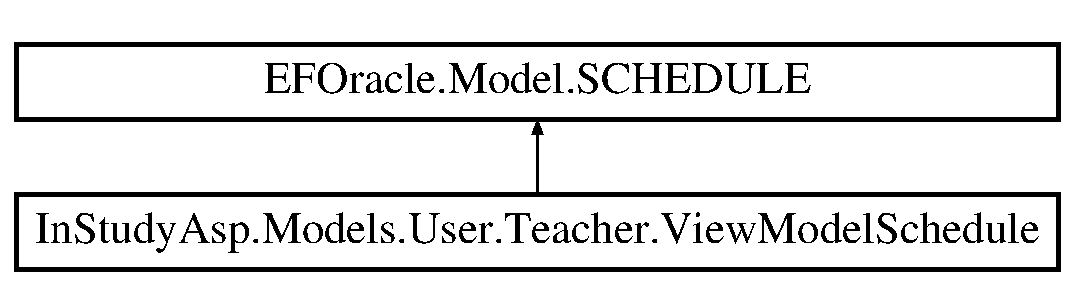
\includegraphics[height=2.000000cm]{class_in_study_asp_1_1_models_1_1_user_1_1_teacher_1_1_view_model_schedule}
\end{center}
\end{figure}
\subsection*{Public Member Functions}
\begin{DoxyCompactItemize}
\item 
\hyperlink{class_in_study_asp_1_1_models_1_1_user_1_1_teacher_1_1_view_model_schedule_a2a6f9735138119885135e10599792ebc}{View\+Model\+Schedule} (\hyperlink{class_e_f_oracle_1_1_model_1_1_s_c_h_e_d_u_l_e}{S\+C\+H\+E\+D\+U\+LE} \+\_\+schedule, \hyperlink{interface_repo_1_1_common_1_1_i_generic_repository}{I\+Generic\+Repository}$<$ \hyperlink{class_e_f_oracle_1_1_model_1_1_s_c_h_e_d_u_l_e}{S\+C\+H\+E\+D\+U\+LE} $>$ \+\_\+repo\+Schedule, \hyperlink{interface_repo_1_1_common_1_1_i_generic_repository}{I\+Generic\+Repository}$<$ \hyperlink{class_e_f_oracle_1_1_model_1_1_d_i_s_c_i_p_l_i_n_e}{D\+I\+S\+C\+I\+P\+L\+I\+NE} $>$ \+\_\+repo\+Discipline, \hyperlink{interface_repo_1_1_common_1_1_i_generic_repository}{I\+Generic\+Repository}$<$ \hyperlink{class_e_f_oracle_1_1_model_1_1_g_r_o_u_p}{G\+R\+O\+UP} $>$ \+\_\+repo\+Group)
\begin{DoxyCompactList}\small\item\em C\+T\+OR Initialization from S\+C\+H\+E\+D\+U\+LE. \end{DoxyCompactList}\item 
\hyperlink{class_in_study_asp_1_1_models_1_1_user_1_1_teacher_1_1_view_model_schedule_aedd00ac53d0f727aa23665f21bf2db92}{View\+Model\+Schedule} ()
\item 
Date\+Time \hyperlink{class_in_study_asp_1_1_models_1_1_user_1_1_teacher_1_1_view_model_schedule_ae5be68b52f4ccbe4231fa9d3b2666048}{Get\+Date\+Time} ()
\begin{DoxyCompactList}\small\item\em Parse Date\+Time from string dd.\+M\+M.\+Y\+Y\+YY hh\+:mm. \end{DoxyCompactList}\end{DoxyCompactItemize}
\subsection*{Static Public Member Functions}
\begin{DoxyCompactItemize}
\item 
static \hyperlink{class_e_f_oracle_1_1_model_1_1_s_c_h_e_d_u_l_e}{S\+C\+H\+E\+D\+U\+LE} \hyperlink{class_in_study_asp_1_1_models_1_1_user_1_1_teacher_1_1_view_model_schedule_a478198b2582f08c56df1711971a08022}{Add\+Or\+Update} (\hyperlink{class_e_f_oracle_1_1_model_1_1_s_c_h_e_d_u_l_e}{S\+C\+H\+E\+D\+U\+LE} \+\_\+oldS, \hyperlink{class_e_f_oracle_1_1_model_1_1_s_c_h_e_d_u_l_e}{S\+C\+H\+E\+D\+U\+LE} \+\_\+newS, \hyperlink{interface_repo_1_1_common_1_1_i_generic_repository}{I\+Generic\+Repository}$<$ \hyperlink{class_e_f_oracle_1_1_model_1_1_s_c_h_e_d_u_l_e}{S\+C\+H\+E\+D\+U\+LE} $>$ schedules)
\begin{DoxyCompactList}\small\item\em Add\+Or\+Update -\/ if S\+C\+H\+E\+D\+U\+LE exist then Add else Update. \end{DoxyCompactList}\end{DoxyCompactItemize}
\subsection*{Public Attributes}
\begin{DoxyCompactItemize}
\item 
Select\+List \hyperlink{class_in_study_asp_1_1_models_1_1_user_1_1_teacher_1_1_view_model_schedule_a3cb89808a0e815b09f1085e3b945066c}{Get\+Discipline} =$>$ new Select\+List( disciplines.\+Union(repo\+Discipline.\+Get\+All()), \char`\"{}D\+I\+S\+C\+I\+P\+L\+I\+N\+E\+\_\+\+C\+O\+DE\char`\"{}, \char`\"{}D\+I\+S\+C\+I\+P\+L\+I\+N\+E\+\_\+\+N\+A\+ME\char`\"{}, D\+I\+S\+C\+I\+P\+L\+I\+N\+E\+\_\+\+C\+O\+DE)
\begin{DoxyCompactList}\small\item\em Provide selection Discipline from Select\+List in View. \end{DoxyCompactList}\item 
Select\+List \hyperlink{class_in_study_asp_1_1_models_1_1_user_1_1_teacher_1_1_view_model_schedule_a16df99554d08b246ecfa66acb8a6238c}{Get\+Group} =$>$ new Select\+List(groups.\+Union(repo\+Group.\+Get\+All()), \char`\"{}G\+R\+O\+U\+P\+\_\+\+C\+O\+DE\char`\"{}, \char`\"{}\hyperlink{class_e_f_oracle_1_1_model_1_1_s_c_h_e_d_u_l_e_aa0b33a5dbbf6c590afd18a5589e5427f}{G\+R\+O\+U\+P\+\_\+\+C\+O\+DE}\char`\"{}, G\+R\+O\+U\+P\+\_\+\+C\+O\+DE)
\begin{DoxyCompactList}\small\item\em Provide selection Group from Select\+List in View. \end{DoxyCompactList}\end{DoxyCompactItemize}
\subsection*{Properties}
\begin{DoxyCompactItemize}
\item 
int \hyperlink{class_in_study_asp_1_1_models_1_1_user_1_1_teacher_1_1_view_model_schedule_a8de805afbeab5943816641787f787071}{Schedule\+Room}\hspace{0.3cm}{\ttfamily  \mbox{[}get, set\mbox{]}}
\begin{DoxyCompactList}\small\item\em To convert decimal S\+C\+H\+E\+D\+U\+L\+E\+\_\+\+R\+O\+OM to int for view. \end{DoxyCompactList}\item 
string \hyperlink{class_in_study_asp_1_1_models_1_1_user_1_1_teacher_1_1_view_model_schedule_a8263bc709f1e63fd8d4406f1ad2d9f6f}{Old\+ID}\hspace{0.3cm}{\ttfamily  \mbox{[}get, set\mbox{]}}
\begin{DoxyCompactList}\small\item\em Store json of unchanged S\+C\+H\+E\+D\+U\+LE. \end{DoxyCompactList}\item 
string \hyperlink{class_in_study_asp_1_1_models_1_1_user_1_1_teacher_1_1_view_model_schedule_a36455e485d079b033236de1c892adb8f}{S\+C\+H\+E\+D\+U\+L\+E\+\_\+\+D\+A\+T\+E2}\hspace{0.3cm}{\ttfamily  \mbox{[}get, set\mbox{]}}
\begin{DoxyCompactList}\small\item\em To prevent hand edit of main field. \end{DoxyCompactList}\item 
I\+Enumerable$<$ \hyperlink{class_e_f_oracle_1_1_model_1_1_d_i_s_c_i_p_l_i_n_e}{D\+I\+S\+C\+I\+P\+L\+I\+NE} $>$ \hyperlink{class_in_study_asp_1_1_models_1_1_user_1_1_teacher_1_1_view_model_schedule_ab78fd27cfd27e6f1be6c414acff93b41}{disciplines}\hspace{0.3cm}{\ttfamily  \mbox{[}get\mbox{]}}
\item 
I\+Enumerable$<$ \hyperlink{class_e_f_oracle_1_1_model_1_1_g_r_o_u_p}{G\+R\+O\+UP} $>$ \hyperlink{class_in_study_asp_1_1_models_1_1_user_1_1_teacher_1_1_view_model_schedule_a51d1addd43459362469f427a00436f50}{groups}\hspace{0.3cm}{\ttfamily  \mbox{[}get\mbox{]}}
\end{DoxyCompactItemize}
\subsection*{Private Attributes}
\begin{DoxyCompactItemize}
\item 
\hyperlink{interface_repo_1_1_common_1_1_i_generic_repository}{I\+Generic\+Repository}$<$ \hyperlink{class_e_f_oracle_1_1_model_1_1_d_i_s_c_i_p_l_i_n_e}{D\+I\+S\+C\+I\+P\+L\+I\+NE} $>$ \hyperlink{class_in_study_asp_1_1_models_1_1_user_1_1_teacher_1_1_view_model_schedule_af83b9134a2fb82ac95d54bae3048b634}{repo\+Discipline}
\item 
\hyperlink{interface_repo_1_1_common_1_1_i_generic_repository}{I\+Generic\+Repository}$<$ \hyperlink{class_e_f_oracle_1_1_model_1_1_g_r_o_u_p}{G\+R\+O\+UP} $>$ \hyperlink{class_in_study_asp_1_1_models_1_1_user_1_1_teacher_1_1_view_model_schedule_ae6fcb15e9c68b57ded9300e873d5e1fc}{repo\+Group}
\item 
\hyperlink{interface_repo_1_1_common_1_1_i_generic_repository}{I\+Generic\+Repository}$<$ \hyperlink{class_e_f_oracle_1_1_model_1_1_s_c_h_e_d_u_l_e}{S\+C\+H\+E\+D\+U\+LE} $>$ \hyperlink{class_in_study_asp_1_1_models_1_1_user_1_1_teacher_1_1_view_model_schedule_a6c85660782fd7647ca942cc759988872}{repo\+Schedule}
\end{DoxyCompactItemize}


\subsection{Detailed Description}
View\+Model for Schedule\+Controller. 

\subsection{Constructor \& Destructor Documentation}
\mbox{\Hypertarget{class_in_study_asp_1_1_models_1_1_user_1_1_teacher_1_1_view_model_schedule_a2a6f9735138119885135e10599792ebc}\label{class_in_study_asp_1_1_models_1_1_user_1_1_teacher_1_1_view_model_schedule_a2a6f9735138119885135e10599792ebc}} 
\index{In\+Study\+Asp\+::\+Models\+::\+User\+::\+Teacher\+::\+View\+Model\+Schedule@{In\+Study\+Asp\+::\+Models\+::\+User\+::\+Teacher\+::\+View\+Model\+Schedule}!View\+Model\+Schedule@{View\+Model\+Schedule}}
\index{View\+Model\+Schedule@{View\+Model\+Schedule}!In\+Study\+Asp\+::\+Models\+::\+User\+::\+Teacher\+::\+View\+Model\+Schedule@{In\+Study\+Asp\+::\+Models\+::\+User\+::\+Teacher\+::\+View\+Model\+Schedule}}
\subsubsection{\texorpdfstring{View\+Model\+Schedule()}{ViewModelSchedule()}\hspace{0.1cm}{\footnotesize\ttfamily [1/2]}}
{\footnotesize\ttfamily In\+Study\+Asp.\+Models.\+User.\+Teacher.\+View\+Model\+Schedule.\+View\+Model\+Schedule (\begin{DoxyParamCaption}\item[{\hyperlink{class_e_f_oracle_1_1_model_1_1_s_c_h_e_d_u_l_e}{S\+C\+H\+E\+D\+U\+LE}}]{\+\_\+schedule,  }\item[{\hyperlink{interface_repo_1_1_common_1_1_i_generic_repository}{I\+Generic\+Repository}$<$ \hyperlink{class_e_f_oracle_1_1_model_1_1_s_c_h_e_d_u_l_e}{S\+C\+H\+E\+D\+U\+LE} $>$}]{\+\_\+repo\+Schedule,  }\item[{\hyperlink{interface_repo_1_1_common_1_1_i_generic_repository}{I\+Generic\+Repository}$<$ \hyperlink{class_e_f_oracle_1_1_model_1_1_d_i_s_c_i_p_l_i_n_e}{D\+I\+S\+C\+I\+P\+L\+I\+NE} $>$}]{\+\_\+repo\+Discipline,  }\item[{\hyperlink{interface_repo_1_1_common_1_1_i_generic_repository}{I\+Generic\+Repository}$<$ \hyperlink{class_e_f_oracle_1_1_model_1_1_g_r_o_u_p}{G\+R\+O\+UP} $>$}]{\+\_\+repo\+Group }\end{DoxyParamCaption})}



C\+T\+OR Initialization from S\+C\+H\+E\+D\+U\+LE. 

\mbox{\Hypertarget{class_in_study_asp_1_1_models_1_1_user_1_1_teacher_1_1_view_model_schedule_aedd00ac53d0f727aa23665f21bf2db92}\label{class_in_study_asp_1_1_models_1_1_user_1_1_teacher_1_1_view_model_schedule_aedd00ac53d0f727aa23665f21bf2db92}} 
\index{In\+Study\+Asp\+::\+Models\+::\+User\+::\+Teacher\+::\+View\+Model\+Schedule@{In\+Study\+Asp\+::\+Models\+::\+User\+::\+Teacher\+::\+View\+Model\+Schedule}!View\+Model\+Schedule@{View\+Model\+Schedule}}
\index{View\+Model\+Schedule@{View\+Model\+Schedule}!In\+Study\+Asp\+::\+Models\+::\+User\+::\+Teacher\+::\+View\+Model\+Schedule@{In\+Study\+Asp\+::\+Models\+::\+User\+::\+Teacher\+::\+View\+Model\+Schedule}}
\subsubsection{\texorpdfstring{View\+Model\+Schedule()}{ViewModelSchedule()}\hspace{0.1cm}{\footnotesize\ttfamily [2/2]}}
{\footnotesize\ttfamily In\+Study\+Asp.\+Models.\+User.\+Teacher.\+View\+Model\+Schedule.\+View\+Model\+Schedule (\begin{DoxyParamCaption}{ }\end{DoxyParamCaption})}



\subsection{Member Function Documentation}
\mbox{\Hypertarget{class_in_study_asp_1_1_models_1_1_user_1_1_teacher_1_1_view_model_schedule_a478198b2582f08c56df1711971a08022}\label{class_in_study_asp_1_1_models_1_1_user_1_1_teacher_1_1_view_model_schedule_a478198b2582f08c56df1711971a08022}} 
\index{In\+Study\+Asp\+::\+Models\+::\+User\+::\+Teacher\+::\+View\+Model\+Schedule@{In\+Study\+Asp\+::\+Models\+::\+User\+::\+Teacher\+::\+View\+Model\+Schedule}!Add\+Or\+Update@{Add\+Or\+Update}}
\index{Add\+Or\+Update@{Add\+Or\+Update}!In\+Study\+Asp\+::\+Models\+::\+User\+::\+Teacher\+::\+View\+Model\+Schedule@{In\+Study\+Asp\+::\+Models\+::\+User\+::\+Teacher\+::\+View\+Model\+Schedule}}
\subsubsection{\texorpdfstring{Add\+Or\+Update()}{AddOrUpdate()}}
{\footnotesize\ttfamily static \hyperlink{class_e_f_oracle_1_1_model_1_1_s_c_h_e_d_u_l_e}{S\+C\+H\+E\+D\+U\+LE} In\+Study\+Asp.\+Models.\+User.\+Teacher.\+View\+Model\+Schedule.\+Add\+Or\+Update (\begin{DoxyParamCaption}\item[{\hyperlink{class_e_f_oracle_1_1_model_1_1_s_c_h_e_d_u_l_e}{S\+C\+H\+E\+D\+U\+LE}}]{\+\_\+oldS,  }\item[{\hyperlink{class_e_f_oracle_1_1_model_1_1_s_c_h_e_d_u_l_e}{S\+C\+H\+E\+D\+U\+LE}}]{\+\_\+newS,  }\item[{\hyperlink{interface_repo_1_1_common_1_1_i_generic_repository}{I\+Generic\+Repository}$<$ \hyperlink{class_e_f_oracle_1_1_model_1_1_s_c_h_e_d_u_l_e}{S\+C\+H\+E\+D\+U\+LE} $>$}]{schedules }\end{DoxyParamCaption})\hspace{0.3cm}{\ttfamily [static]}}



Add\+Or\+Update -\/ if S\+C\+H\+E\+D\+U\+LE exist then Add else Update. 

\mbox{\Hypertarget{class_in_study_asp_1_1_models_1_1_user_1_1_teacher_1_1_view_model_schedule_ae5be68b52f4ccbe4231fa9d3b2666048}\label{class_in_study_asp_1_1_models_1_1_user_1_1_teacher_1_1_view_model_schedule_ae5be68b52f4ccbe4231fa9d3b2666048}} 
\index{In\+Study\+Asp\+::\+Models\+::\+User\+::\+Teacher\+::\+View\+Model\+Schedule@{In\+Study\+Asp\+::\+Models\+::\+User\+::\+Teacher\+::\+View\+Model\+Schedule}!Get\+Date\+Time@{Get\+Date\+Time}}
\index{Get\+Date\+Time@{Get\+Date\+Time}!In\+Study\+Asp\+::\+Models\+::\+User\+::\+Teacher\+::\+View\+Model\+Schedule@{In\+Study\+Asp\+::\+Models\+::\+User\+::\+Teacher\+::\+View\+Model\+Schedule}}
\subsubsection{\texorpdfstring{Get\+Date\+Time()}{GetDateTime()}}
{\footnotesize\ttfamily Date\+Time In\+Study\+Asp.\+Models.\+User.\+Teacher.\+View\+Model\+Schedule.\+Get\+Date\+Time (\begin{DoxyParamCaption}{ }\end{DoxyParamCaption})}



Parse Date\+Time from string dd.\+M\+M.\+Y\+Y\+YY hh\+:mm. 



\subsection{Member Data Documentation}
\mbox{\Hypertarget{class_in_study_asp_1_1_models_1_1_user_1_1_teacher_1_1_view_model_schedule_a3cb89808a0e815b09f1085e3b945066c}\label{class_in_study_asp_1_1_models_1_1_user_1_1_teacher_1_1_view_model_schedule_a3cb89808a0e815b09f1085e3b945066c}} 
\index{In\+Study\+Asp\+::\+Models\+::\+User\+::\+Teacher\+::\+View\+Model\+Schedule@{In\+Study\+Asp\+::\+Models\+::\+User\+::\+Teacher\+::\+View\+Model\+Schedule}!Get\+Discipline@{Get\+Discipline}}
\index{Get\+Discipline@{Get\+Discipline}!In\+Study\+Asp\+::\+Models\+::\+User\+::\+Teacher\+::\+View\+Model\+Schedule@{In\+Study\+Asp\+::\+Models\+::\+User\+::\+Teacher\+::\+View\+Model\+Schedule}}
\subsubsection{\texorpdfstring{Get\+Discipline}{GetDiscipline}}
{\footnotesize\ttfamily Select\+List In\+Study\+Asp.\+Models.\+User.\+Teacher.\+View\+Model\+Schedule.\+Get\+Discipline =$>$ new Select\+List( disciplines.\+Union(repo\+Discipline.\+Get\+All()), \char`\"{}D\+I\+S\+C\+I\+P\+L\+I\+N\+E\+\_\+\+C\+O\+DE\char`\"{}, \char`\"{}D\+I\+S\+C\+I\+P\+L\+I\+N\+E\+\_\+\+N\+A\+ME\char`\"{}, D\+I\+S\+C\+I\+P\+L\+I\+N\+E\+\_\+\+C\+O\+DE)}



Provide selection Discipline from Select\+List in View. 

\mbox{\Hypertarget{class_in_study_asp_1_1_models_1_1_user_1_1_teacher_1_1_view_model_schedule_a16df99554d08b246ecfa66acb8a6238c}\label{class_in_study_asp_1_1_models_1_1_user_1_1_teacher_1_1_view_model_schedule_a16df99554d08b246ecfa66acb8a6238c}} 
\index{In\+Study\+Asp\+::\+Models\+::\+User\+::\+Teacher\+::\+View\+Model\+Schedule@{In\+Study\+Asp\+::\+Models\+::\+User\+::\+Teacher\+::\+View\+Model\+Schedule}!Get\+Group@{Get\+Group}}
\index{Get\+Group@{Get\+Group}!In\+Study\+Asp\+::\+Models\+::\+User\+::\+Teacher\+::\+View\+Model\+Schedule@{In\+Study\+Asp\+::\+Models\+::\+User\+::\+Teacher\+::\+View\+Model\+Schedule}}
\subsubsection{\texorpdfstring{Get\+Group}{GetGroup}}
{\footnotesize\ttfamily Select\+List In\+Study\+Asp.\+Models.\+User.\+Teacher.\+View\+Model\+Schedule.\+Get\+Group =$>$ new Select\+List(groups.\+Union(repo\+Group.\+Get\+All()), \char`\"{}G\+R\+O\+U\+P\+\_\+\+C\+O\+DE\char`\"{}, \char`\"{}\hyperlink{class_e_f_oracle_1_1_model_1_1_s_c_h_e_d_u_l_e_aa0b33a5dbbf6c590afd18a5589e5427f}{G\+R\+O\+U\+P\+\_\+\+C\+O\+DE}\char`\"{}, G\+R\+O\+U\+P\+\_\+\+C\+O\+DE)}



Provide selection Group from Select\+List in View. 

\mbox{\Hypertarget{class_in_study_asp_1_1_models_1_1_user_1_1_teacher_1_1_view_model_schedule_af83b9134a2fb82ac95d54bae3048b634}\label{class_in_study_asp_1_1_models_1_1_user_1_1_teacher_1_1_view_model_schedule_af83b9134a2fb82ac95d54bae3048b634}} 
\index{In\+Study\+Asp\+::\+Models\+::\+User\+::\+Teacher\+::\+View\+Model\+Schedule@{In\+Study\+Asp\+::\+Models\+::\+User\+::\+Teacher\+::\+View\+Model\+Schedule}!repo\+Discipline@{repo\+Discipline}}
\index{repo\+Discipline@{repo\+Discipline}!In\+Study\+Asp\+::\+Models\+::\+User\+::\+Teacher\+::\+View\+Model\+Schedule@{In\+Study\+Asp\+::\+Models\+::\+User\+::\+Teacher\+::\+View\+Model\+Schedule}}
\subsubsection{\texorpdfstring{repo\+Discipline}{repoDiscipline}}
{\footnotesize\ttfamily \hyperlink{interface_repo_1_1_common_1_1_i_generic_repository}{I\+Generic\+Repository}$<$\hyperlink{class_e_f_oracle_1_1_model_1_1_d_i_s_c_i_p_l_i_n_e}{D\+I\+S\+C\+I\+P\+L\+I\+NE}$>$ In\+Study\+Asp.\+Models.\+User.\+Teacher.\+View\+Model\+Schedule.\+repo\+Discipline\hspace{0.3cm}{\ttfamily [private]}}

\mbox{\Hypertarget{class_in_study_asp_1_1_models_1_1_user_1_1_teacher_1_1_view_model_schedule_ae6fcb15e9c68b57ded9300e873d5e1fc}\label{class_in_study_asp_1_1_models_1_1_user_1_1_teacher_1_1_view_model_schedule_ae6fcb15e9c68b57ded9300e873d5e1fc}} 
\index{In\+Study\+Asp\+::\+Models\+::\+User\+::\+Teacher\+::\+View\+Model\+Schedule@{In\+Study\+Asp\+::\+Models\+::\+User\+::\+Teacher\+::\+View\+Model\+Schedule}!repo\+Group@{repo\+Group}}
\index{repo\+Group@{repo\+Group}!In\+Study\+Asp\+::\+Models\+::\+User\+::\+Teacher\+::\+View\+Model\+Schedule@{In\+Study\+Asp\+::\+Models\+::\+User\+::\+Teacher\+::\+View\+Model\+Schedule}}
\subsubsection{\texorpdfstring{repo\+Group}{repoGroup}}
{\footnotesize\ttfamily \hyperlink{interface_repo_1_1_common_1_1_i_generic_repository}{I\+Generic\+Repository}$<$\hyperlink{class_e_f_oracle_1_1_model_1_1_g_r_o_u_p}{G\+R\+O\+UP}$>$ In\+Study\+Asp.\+Models.\+User.\+Teacher.\+View\+Model\+Schedule.\+repo\+Group\hspace{0.3cm}{\ttfamily [private]}}

\mbox{\Hypertarget{class_in_study_asp_1_1_models_1_1_user_1_1_teacher_1_1_view_model_schedule_a6c85660782fd7647ca942cc759988872}\label{class_in_study_asp_1_1_models_1_1_user_1_1_teacher_1_1_view_model_schedule_a6c85660782fd7647ca942cc759988872}} 
\index{In\+Study\+Asp\+::\+Models\+::\+User\+::\+Teacher\+::\+View\+Model\+Schedule@{In\+Study\+Asp\+::\+Models\+::\+User\+::\+Teacher\+::\+View\+Model\+Schedule}!repo\+Schedule@{repo\+Schedule}}
\index{repo\+Schedule@{repo\+Schedule}!In\+Study\+Asp\+::\+Models\+::\+User\+::\+Teacher\+::\+View\+Model\+Schedule@{In\+Study\+Asp\+::\+Models\+::\+User\+::\+Teacher\+::\+View\+Model\+Schedule}}
\subsubsection{\texorpdfstring{repo\+Schedule}{repoSchedule}}
{\footnotesize\ttfamily \hyperlink{interface_repo_1_1_common_1_1_i_generic_repository}{I\+Generic\+Repository}$<$\hyperlink{class_e_f_oracle_1_1_model_1_1_s_c_h_e_d_u_l_e}{S\+C\+H\+E\+D\+U\+LE}$>$ In\+Study\+Asp.\+Models.\+User.\+Teacher.\+View\+Model\+Schedule.\+repo\+Schedule\hspace{0.3cm}{\ttfamily [private]}}



\subsection{Property Documentation}
\mbox{\Hypertarget{class_in_study_asp_1_1_models_1_1_user_1_1_teacher_1_1_view_model_schedule_ab78fd27cfd27e6f1be6c414acff93b41}\label{class_in_study_asp_1_1_models_1_1_user_1_1_teacher_1_1_view_model_schedule_ab78fd27cfd27e6f1be6c414acff93b41}} 
\index{In\+Study\+Asp\+::\+Models\+::\+User\+::\+Teacher\+::\+View\+Model\+Schedule@{In\+Study\+Asp\+::\+Models\+::\+User\+::\+Teacher\+::\+View\+Model\+Schedule}!disciplines@{disciplines}}
\index{disciplines@{disciplines}!In\+Study\+Asp\+::\+Models\+::\+User\+::\+Teacher\+::\+View\+Model\+Schedule@{In\+Study\+Asp\+::\+Models\+::\+User\+::\+Teacher\+::\+View\+Model\+Schedule}}
\subsubsection{\texorpdfstring{disciplines}{disciplines}}
{\footnotesize\ttfamily I\+Enumerable$<$\hyperlink{class_e_f_oracle_1_1_model_1_1_d_i_s_c_i_p_l_i_n_e}{D\+I\+S\+C\+I\+P\+L\+I\+NE}$>$ In\+Study\+Asp.\+Models.\+User.\+Teacher.\+View\+Model\+Schedule.\+disciplines\hspace{0.3cm}{\ttfamily [get]}, {\ttfamily [private]}}

\mbox{\Hypertarget{class_in_study_asp_1_1_models_1_1_user_1_1_teacher_1_1_view_model_schedule_a51d1addd43459362469f427a00436f50}\label{class_in_study_asp_1_1_models_1_1_user_1_1_teacher_1_1_view_model_schedule_a51d1addd43459362469f427a00436f50}} 
\index{In\+Study\+Asp\+::\+Models\+::\+User\+::\+Teacher\+::\+View\+Model\+Schedule@{In\+Study\+Asp\+::\+Models\+::\+User\+::\+Teacher\+::\+View\+Model\+Schedule}!groups@{groups}}
\index{groups@{groups}!In\+Study\+Asp\+::\+Models\+::\+User\+::\+Teacher\+::\+View\+Model\+Schedule@{In\+Study\+Asp\+::\+Models\+::\+User\+::\+Teacher\+::\+View\+Model\+Schedule}}
\subsubsection{\texorpdfstring{groups}{groups}}
{\footnotesize\ttfamily I\+Enumerable$<$\hyperlink{class_e_f_oracle_1_1_model_1_1_g_r_o_u_p}{G\+R\+O\+UP}$>$ In\+Study\+Asp.\+Models.\+User.\+Teacher.\+View\+Model\+Schedule.\+groups\hspace{0.3cm}{\ttfamily [get]}, {\ttfamily [private]}}

\mbox{\Hypertarget{class_in_study_asp_1_1_models_1_1_user_1_1_teacher_1_1_view_model_schedule_a8263bc709f1e63fd8d4406f1ad2d9f6f}\label{class_in_study_asp_1_1_models_1_1_user_1_1_teacher_1_1_view_model_schedule_a8263bc709f1e63fd8d4406f1ad2d9f6f}} 
\index{In\+Study\+Asp\+::\+Models\+::\+User\+::\+Teacher\+::\+View\+Model\+Schedule@{In\+Study\+Asp\+::\+Models\+::\+User\+::\+Teacher\+::\+View\+Model\+Schedule}!Old\+ID@{Old\+ID}}
\index{Old\+ID@{Old\+ID}!In\+Study\+Asp\+::\+Models\+::\+User\+::\+Teacher\+::\+View\+Model\+Schedule@{In\+Study\+Asp\+::\+Models\+::\+User\+::\+Teacher\+::\+View\+Model\+Schedule}}
\subsubsection{\texorpdfstring{Old\+ID}{OldID}}
{\footnotesize\ttfamily string In\+Study\+Asp.\+Models.\+User.\+Teacher.\+View\+Model\+Schedule.\+Old\+ID\hspace{0.3cm}{\ttfamily [get]}, {\ttfamily [set]}}



Store json of unchanged S\+C\+H\+E\+D\+U\+LE. 

\mbox{\Hypertarget{class_in_study_asp_1_1_models_1_1_user_1_1_teacher_1_1_view_model_schedule_a36455e485d079b033236de1c892adb8f}\label{class_in_study_asp_1_1_models_1_1_user_1_1_teacher_1_1_view_model_schedule_a36455e485d079b033236de1c892adb8f}} 
\index{In\+Study\+Asp\+::\+Models\+::\+User\+::\+Teacher\+::\+View\+Model\+Schedule@{In\+Study\+Asp\+::\+Models\+::\+User\+::\+Teacher\+::\+View\+Model\+Schedule}!S\+C\+H\+E\+D\+U\+L\+E\+\_\+\+D\+A\+T\+E2@{S\+C\+H\+E\+D\+U\+L\+E\+\_\+\+D\+A\+T\+E2}}
\index{S\+C\+H\+E\+D\+U\+L\+E\+\_\+\+D\+A\+T\+E2@{S\+C\+H\+E\+D\+U\+L\+E\+\_\+\+D\+A\+T\+E2}!In\+Study\+Asp\+::\+Models\+::\+User\+::\+Teacher\+::\+View\+Model\+Schedule@{In\+Study\+Asp\+::\+Models\+::\+User\+::\+Teacher\+::\+View\+Model\+Schedule}}
\subsubsection{\texorpdfstring{S\+C\+H\+E\+D\+U\+L\+E\+\_\+\+D\+A\+T\+E2}{SCHEDULE\_DATE2}}
{\footnotesize\ttfamily string In\+Study\+Asp.\+Models.\+User.\+Teacher.\+View\+Model\+Schedule.\+S\+C\+H\+E\+D\+U\+L\+E\+\_\+\+D\+A\+T\+E2\hspace{0.3cm}{\ttfamily [get]}, {\ttfamily [set]}}



To prevent hand edit of main field. 

\mbox{\Hypertarget{class_in_study_asp_1_1_models_1_1_user_1_1_teacher_1_1_view_model_schedule_a8de805afbeab5943816641787f787071}\label{class_in_study_asp_1_1_models_1_1_user_1_1_teacher_1_1_view_model_schedule_a8de805afbeab5943816641787f787071}} 
\index{In\+Study\+Asp\+::\+Models\+::\+User\+::\+Teacher\+::\+View\+Model\+Schedule@{In\+Study\+Asp\+::\+Models\+::\+User\+::\+Teacher\+::\+View\+Model\+Schedule}!Schedule\+Room@{Schedule\+Room}}
\index{Schedule\+Room@{Schedule\+Room}!In\+Study\+Asp\+::\+Models\+::\+User\+::\+Teacher\+::\+View\+Model\+Schedule@{In\+Study\+Asp\+::\+Models\+::\+User\+::\+Teacher\+::\+View\+Model\+Schedule}}
\subsubsection{\texorpdfstring{Schedule\+Room}{ScheduleRoom}}
{\footnotesize\ttfamily int In\+Study\+Asp.\+Models.\+User.\+Teacher.\+View\+Model\+Schedule.\+Schedule\+Room\hspace{0.3cm}{\ttfamily [get]}, {\ttfamily [set]}}



To convert decimal S\+C\+H\+E\+D\+U\+L\+E\+\_\+\+R\+O\+OM to int for view. 



The documentation for this class was generated from the following file\+:\begin{DoxyCompactItemize}
\item 
D\+:/\+\_\+\+W\+O\+R\+K/\+\_\+\+S\+T\+E\+P/\+In\+Study\+Asp/\+In\+Study\+Asp/\+Models/\+User/\+Teacher/\hyperlink{_view_model_schedule_8cs}{View\+Model\+Schedule.\+cs}\end{DoxyCompactItemize}

\chapter{File Documentation}
\hypertarget{db_context_8cs}{}\section{D\+:/\+\_\+\+W\+O\+R\+K/\+\_\+\+S\+T\+E\+P/\+In\+Study\+Asp/\+E\+F\+Oracle/\+Model/db\+Context.cs File Reference}
\label{db_context_8cs}\index{D\+:/\+\_\+\+W\+O\+R\+K/\+\_\+\+S\+T\+E\+P/\+In\+Study\+Asp/\+E\+F\+Oracle/\+Model/db\+Context.\+cs@{D\+:/\+\_\+\+W\+O\+R\+K/\+\_\+\+S\+T\+E\+P/\+In\+Study\+Asp/\+E\+F\+Oracle/\+Model/db\+Context.\+cs}}
\subsection*{Classes}
\begin{DoxyCompactItemize}
\item 
class \hyperlink{class_e_f_oracle_1_1_model_1_1db_context}{E\+F\+Oracle.\+Model.\+db\+Context}
\end{DoxyCompactItemize}
\subsection*{Namespaces}
\begin{DoxyCompactItemize}
\item 
namespace \hyperlink{namespace_e_f_oracle_1_1_model}{E\+F\+Oracle.\+Model}
\end{DoxyCompactItemize}

\hypertarget{_d_i_s_c_i_p_l_i_n_e_8cs}{}\section{D\+:/\+\_\+\+W\+O\+R\+K/\+\_\+\+S\+T\+E\+P/\+In\+Study\+Asp/\+E\+F\+Oracle/\+Model/\+D\+I\+S\+C\+I\+P\+L\+I\+NE.cs File Reference}
\label{_d_i_s_c_i_p_l_i_n_e_8cs}\index{D\+:/\+\_\+\+W\+O\+R\+K/\+\_\+\+S\+T\+E\+P/\+In\+Study\+Asp/\+E\+F\+Oracle/\+Model/\+D\+I\+S\+C\+I\+P\+L\+I\+N\+E.\+cs@{D\+:/\+\_\+\+W\+O\+R\+K/\+\_\+\+S\+T\+E\+P/\+In\+Study\+Asp/\+E\+F\+Oracle/\+Model/\+D\+I\+S\+C\+I\+P\+L\+I\+N\+E.\+cs}}
\subsection*{Classes}
\begin{DoxyCompactItemize}
\item 
class \hyperlink{class_e_f_oracle_1_1_model_1_1_d_i_s_c_i_p_l_i_n_e}{E\+F\+Oracle.\+Model.\+D\+I\+S\+C\+I\+P\+L\+I\+NE}
\end{DoxyCompactItemize}
\subsection*{Namespaces}
\begin{DoxyCompactItemize}
\item 
namespace \hyperlink{namespace_e_f_oracle_1_1_model}{E\+F\+Oracle.\+Model}
\end{DoxyCompactItemize}

\hypertarget{_extended_2_s_c_h_e_d_u_l_e_8cs}{}\section{D\+:/\+\_\+\+W\+O\+R\+K/\+\_\+\+S\+T\+E\+P/\+In\+Study\+Asp/\+E\+F\+Oracle/\+Model/\+Extended/\+S\+C\+H\+E\+D\+U\+LE.cs File Reference}
\label{_extended_2_s_c_h_e_d_u_l_e_8cs}\index{D\+:/\+\_\+\+W\+O\+R\+K/\+\_\+\+S\+T\+E\+P/\+In\+Study\+Asp/\+E\+F\+Oracle/\+Model/\+Extended/\+S\+C\+H\+E\+D\+U\+L\+E.\+cs@{D\+:/\+\_\+\+W\+O\+R\+K/\+\_\+\+S\+T\+E\+P/\+In\+Study\+Asp/\+E\+F\+Oracle/\+Model/\+Extended/\+S\+C\+H\+E\+D\+U\+L\+E.\+cs}}
\subsection*{Classes}
\begin{DoxyCompactItemize}
\item 
class \hyperlink{class_e_f_oracle_1_1_model_1_1_s_c_h_e_d_u_l_e}{E\+F\+Oracle.\+Model.\+S\+C\+H\+E\+D\+U\+LE}
\begin{DoxyCompactList}\small\item\em Specifying view metadata for \hyperlink{class_e_f_oracle_1_1_model_1_1_s_c_h_e_d_u_l_e}{S\+C\+H\+E\+D\+U\+LE} class. \end{DoxyCompactList}\item 
class \hyperlink{class_e_f_oracle_1_1_model_1_1_schedule_metadata}{E\+F\+Oracle.\+Model.\+Schedule\+Metadata}
\end{DoxyCompactItemize}
\subsection*{Namespaces}
\begin{DoxyCompactItemize}
\item 
namespace \hyperlink{namespace_e_f_oracle_1_1_model}{E\+F\+Oracle.\+Model}
\end{DoxyCompactItemize}

\hypertarget{_s_c_h_e_d_u_l_e_8cs}{}\section{D\+:/\+\_\+\+W\+O\+R\+K/\+\_\+\+S\+T\+E\+P/\+In\+Study\+Asp/\+E\+F\+Oracle/\+Model/\+S\+C\+H\+E\+D\+U\+LE.cs File Reference}
\label{_s_c_h_e_d_u_l_e_8cs}\index{D\+:/\+\_\+\+W\+O\+R\+K/\+\_\+\+S\+T\+E\+P/\+In\+Study\+Asp/\+E\+F\+Oracle/\+Model/\+S\+C\+H\+E\+D\+U\+L\+E.\+cs@{D\+:/\+\_\+\+W\+O\+R\+K/\+\_\+\+S\+T\+E\+P/\+In\+Study\+Asp/\+E\+F\+Oracle/\+Model/\+S\+C\+H\+E\+D\+U\+L\+E.\+cs}}
\subsection*{Classes}
\begin{DoxyCompactItemize}
\item 
class \hyperlink{class_e_f_oracle_1_1_model_1_1_s_c_h_e_d_u_l_e}{E\+F\+Oracle.\+Model.\+S\+C\+H\+E\+D\+U\+LE}
\begin{DoxyCompactList}\small\item\em Specifying view metadata for \hyperlink{class_e_f_oracle_1_1_model_1_1_s_c_h_e_d_u_l_e}{S\+C\+H\+E\+D\+U\+LE} class. \end{DoxyCompactList}\end{DoxyCompactItemize}
\subsection*{Namespaces}
\begin{DoxyCompactItemize}
\item 
namespace \hyperlink{namespace_e_f_oracle_1_1_model}{E\+F\+Oracle.\+Model}
\end{DoxyCompactItemize}

\hypertarget{_f_a_q_8cs}{}\section{D\+:/\+\_\+\+W\+O\+R\+K/\+\_\+\+S\+T\+E\+P/\+In\+Study\+Asp/\+E\+F\+Oracle/\+Model/\+F\+AQ.cs File Reference}
\label{_f_a_q_8cs}\index{D\+:/\+\_\+\+W\+O\+R\+K/\+\_\+\+S\+T\+E\+P/\+In\+Study\+Asp/\+E\+F\+Oracle/\+Model/\+F\+A\+Q.\+cs@{D\+:/\+\_\+\+W\+O\+R\+K/\+\_\+\+S\+T\+E\+P/\+In\+Study\+Asp/\+E\+F\+Oracle/\+Model/\+F\+A\+Q.\+cs}}
\subsection*{Classes}
\begin{DoxyCompactItemize}
\item 
class \hyperlink{class_e_f_oracle_1_1_model_1_1_f_a_q}{E\+F\+Oracle.\+Model.\+F\+AQ}
\end{DoxyCompactItemize}
\subsection*{Namespaces}
\begin{DoxyCompactItemize}
\item 
namespace \hyperlink{namespace_e_f_oracle_1_1_model}{E\+F\+Oracle.\+Model}
\end{DoxyCompactItemize}

\hypertarget{_g_r_o_u_p_8cs}{}\section{D\+:/\+\_\+\+W\+O\+R\+K/\+\_\+\+S\+T\+E\+P/\+In\+Study\+Asp/\+E\+F\+Oracle/\+Model/\+G\+R\+O\+UP.cs File Reference}
\label{_g_r_o_u_p_8cs}\index{D\+:/\+\_\+\+W\+O\+R\+K/\+\_\+\+S\+T\+E\+P/\+In\+Study\+Asp/\+E\+F\+Oracle/\+Model/\+G\+R\+O\+U\+P.\+cs@{D\+:/\+\_\+\+W\+O\+R\+K/\+\_\+\+S\+T\+E\+P/\+In\+Study\+Asp/\+E\+F\+Oracle/\+Model/\+G\+R\+O\+U\+P.\+cs}}
\subsection*{Classes}
\begin{DoxyCompactItemize}
\item 
class \hyperlink{class_e_f_oracle_1_1_model_1_1_g_r_o_u_p}{E\+F\+Oracle.\+Model.\+G\+R\+O\+UP}
\end{DoxyCompactItemize}
\subsection*{Namespaces}
\begin{DoxyCompactItemize}
\item 
namespace \hyperlink{namespace_e_f_oracle_1_1_model}{E\+F\+Oracle.\+Model}
\end{DoxyCompactItemize}

\hypertarget{_s_t_u_d_e_n_t_8cs}{}\section{D\+:/\+\_\+\+W\+O\+R\+K/\+\_\+\+S\+T\+E\+P/\+In\+Study\+Asp/\+E\+F\+Oracle/\+Model/\+S\+T\+U\+D\+E\+NT.cs File Reference}
\label{_s_t_u_d_e_n_t_8cs}\index{D\+:/\+\_\+\+W\+O\+R\+K/\+\_\+\+S\+T\+E\+P/\+In\+Study\+Asp/\+E\+F\+Oracle/\+Model/\+S\+T\+U\+D\+E\+N\+T.\+cs@{D\+:/\+\_\+\+W\+O\+R\+K/\+\_\+\+S\+T\+E\+P/\+In\+Study\+Asp/\+E\+F\+Oracle/\+Model/\+S\+T\+U\+D\+E\+N\+T.\+cs}}
\subsection*{Classes}
\begin{DoxyCompactItemize}
\item 
class \hyperlink{class_e_f_oracle_1_1_model_1_1_s_t_u_d_e_n_t}{E\+F\+Oracle.\+Model.\+S\+T\+U\+D\+E\+NT}
\end{DoxyCompactItemize}
\subsection*{Namespaces}
\begin{DoxyCompactItemize}
\item 
namespace \hyperlink{namespace_e_f_oracle_1_1_model}{E\+F\+Oracle.\+Model}
\end{DoxyCompactItemize}

\hypertarget{_s_t_u_d_e_n_t_w_o_r_k_8cs}{}\section{D\+:/\+\_\+\+W\+O\+R\+K/\+\_\+\+S\+T\+E\+P/\+In\+Study\+Asp/\+E\+F\+Oracle/\+Model/\+S\+T\+U\+D\+E\+N\+T\+W\+O\+RK.cs File Reference}
\label{_s_t_u_d_e_n_t_w_o_r_k_8cs}\index{D\+:/\+\_\+\+W\+O\+R\+K/\+\_\+\+S\+T\+E\+P/\+In\+Study\+Asp/\+E\+F\+Oracle/\+Model/\+S\+T\+U\+D\+E\+N\+T\+W\+O\+R\+K.\+cs@{D\+:/\+\_\+\+W\+O\+R\+K/\+\_\+\+S\+T\+E\+P/\+In\+Study\+Asp/\+E\+F\+Oracle/\+Model/\+S\+T\+U\+D\+E\+N\+T\+W\+O\+R\+K.\+cs}}
\subsection*{Classes}
\begin{DoxyCompactItemize}
\item 
class \hyperlink{class_e_f_oracle_1_1_model_1_1_s_t_u_d_e_n_t_w_o_r_k}{E\+F\+Oracle.\+Model.\+S\+T\+U\+D\+E\+N\+T\+W\+O\+RK}
\end{DoxyCompactItemize}
\subsection*{Namespaces}
\begin{DoxyCompactItemize}
\item 
namespace \hyperlink{namespace_e_f_oracle_1_1_model}{E\+F\+Oracle.\+Model}
\end{DoxyCompactItemize}

\hypertarget{_t_a_s_k_8cs}{}\section{D\+:/\+\_\+\+W\+O\+R\+K/\+\_\+\+S\+T\+E\+P/\+In\+Study\+Asp/\+E\+F\+Oracle/\+Model/\+T\+A\+SK.cs File Reference}
\label{_t_a_s_k_8cs}\index{D\+:/\+\_\+\+W\+O\+R\+K/\+\_\+\+S\+T\+E\+P/\+In\+Study\+Asp/\+E\+F\+Oracle/\+Model/\+T\+A\+S\+K.\+cs@{D\+:/\+\_\+\+W\+O\+R\+K/\+\_\+\+S\+T\+E\+P/\+In\+Study\+Asp/\+E\+F\+Oracle/\+Model/\+T\+A\+S\+K.\+cs}}
\subsection*{Classes}
\begin{DoxyCompactItemize}
\item 
class \hyperlink{class_e_f_oracle_1_1_model_1_1_t_a_s_k}{E\+F\+Oracle.\+Model.\+T\+A\+SK}
\end{DoxyCompactItemize}
\subsection*{Namespaces}
\begin{DoxyCompactItemize}
\item 
namespace \hyperlink{namespace_e_f_oracle_1_1_model}{E\+F\+Oracle.\+Model}
\end{DoxyCompactItemize}

\hypertarget{_t_a_s_k_t_y_p_e_8cs}{}\section{D\+:/\+\_\+\+W\+O\+R\+K/\+\_\+\+S\+T\+E\+P/\+In\+Study\+Asp/\+E\+F\+Oracle/\+Model/\+T\+A\+S\+K\+T\+Y\+PE.cs File Reference}
\label{_t_a_s_k_t_y_p_e_8cs}\index{D\+:/\+\_\+\+W\+O\+R\+K/\+\_\+\+S\+T\+E\+P/\+In\+Study\+Asp/\+E\+F\+Oracle/\+Model/\+T\+A\+S\+K\+T\+Y\+P\+E.\+cs@{D\+:/\+\_\+\+W\+O\+R\+K/\+\_\+\+S\+T\+E\+P/\+In\+Study\+Asp/\+E\+F\+Oracle/\+Model/\+T\+A\+S\+K\+T\+Y\+P\+E.\+cs}}
\subsection*{Classes}
\begin{DoxyCompactItemize}
\item 
class \hyperlink{class_e_f_oracle_1_1_model_1_1_t_a_s_k_t_y_p_e}{E\+F\+Oracle.\+Model.\+T\+A\+S\+K\+T\+Y\+PE}
\end{DoxyCompactItemize}
\subsection*{Namespaces}
\begin{DoxyCompactItemize}
\item 
namespace \hyperlink{namespace_e_f_oracle_1_1_model}{E\+F\+Oracle.\+Model}
\end{DoxyCompactItemize}

\hypertarget{_t_e_a_c_h_e_r_8cs}{}\section{D\+:/\+\_\+\+W\+O\+R\+K/\+\_\+\+S\+T\+E\+P/\+In\+Study\+Asp/\+E\+F\+Oracle/\+Model/\+T\+E\+A\+C\+H\+ER.cs File Reference}
\label{_t_e_a_c_h_e_r_8cs}\index{D\+:/\+\_\+\+W\+O\+R\+K/\+\_\+\+S\+T\+E\+P/\+In\+Study\+Asp/\+E\+F\+Oracle/\+Model/\+T\+E\+A\+C\+H\+E\+R.\+cs@{D\+:/\+\_\+\+W\+O\+R\+K/\+\_\+\+S\+T\+E\+P/\+In\+Study\+Asp/\+E\+F\+Oracle/\+Model/\+T\+E\+A\+C\+H\+E\+R.\+cs}}
\subsection*{Classes}
\begin{DoxyCompactItemize}
\item 
class \hyperlink{class_e_f_oracle_1_1_model_1_1_t_e_a_c_h_e_r}{E\+F\+Oracle.\+Model.\+T\+E\+A\+C\+H\+ER}
\end{DoxyCompactItemize}
\subsection*{Namespaces}
\begin{DoxyCompactItemize}
\item 
namespace \hyperlink{namespace_e_f_oracle_1_1_model}{E\+F\+Oracle.\+Model}
\end{DoxyCompactItemize}

\hypertarget{_u_s_e_r_8cs}{}\section{D\+:/\+\_\+\+W\+O\+R\+K/\+\_\+\+S\+T\+E\+P/\+In\+Study\+Asp/\+E\+F\+Oracle/\+Model/\+U\+S\+ER.cs File Reference}
\label{_u_s_e_r_8cs}\index{D\+:/\+\_\+\+W\+O\+R\+K/\+\_\+\+S\+T\+E\+P/\+In\+Study\+Asp/\+E\+F\+Oracle/\+Model/\+U\+S\+E\+R.\+cs@{D\+:/\+\_\+\+W\+O\+R\+K/\+\_\+\+S\+T\+E\+P/\+In\+Study\+Asp/\+E\+F\+Oracle/\+Model/\+U\+S\+E\+R.\+cs}}
\subsection*{Classes}
\begin{DoxyCompactItemize}
\item 
class \hyperlink{class_e_f_oracle_1_1_model_1_1_u_s_e_r}{E\+F\+Oracle.\+Model.\+U\+S\+ER}
\end{DoxyCompactItemize}
\subsection*{Namespaces}
\begin{DoxyCompactItemize}
\item 
namespace \hyperlink{namespace_e_f_oracle_1_1_model}{E\+F\+Oracle.\+Model}
\end{DoxyCompactItemize}

\hypertarget{_u_s_e_r___s_e_s_s_i_o_n_8cs}{}\section{D\+:/\+\_\+\+W\+O\+R\+K/\+\_\+\+S\+T\+E\+P/\+In\+Study\+Asp/\+E\+F\+Oracle/\+Model/\+U\+S\+E\+R\+\_\+\+S\+E\+S\+S\+I\+ON.cs File Reference}
\label{_u_s_e_r___s_e_s_s_i_o_n_8cs}\index{D\+:/\+\_\+\+W\+O\+R\+K/\+\_\+\+S\+T\+E\+P/\+In\+Study\+Asp/\+E\+F\+Oracle/\+Model/\+U\+S\+E\+R\+\_\+\+S\+E\+S\+S\+I\+O\+N.\+cs@{D\+:/\+\_\+\+W\+O\+R\+K/\+\_\+\+S\+T\+E\+P/\+In\+Study\+Asp/\+E\+F\+Oracle/\+Model/\+U\+S\+E\+R\+\_\+\+S\+E\+S\+S\+I\+O\+N.\+cs}}
\subsection*{Classes}
\begin{DoxyCompactItemize}
\item 
class \hyperlink{class_e_f_oracle_1_1_model_1_1_u_s_e_r___s_e_s_s_i_o_n}{E\+F\+Oracle.\+Model.\+U\+S\+E\+R\+\_\+\+S\+E\+S\+S\+I\+ON}
\end{DoxyCompactItemize}
\subsection*{Namespaces}
\begin{DoxyCompactItemize}
\item 
namespace \hyperlink{namespace_e_f_oracle_1_1_model}{E\+F\+Oracle.\+Model}
\end{DoxyCompactItemize}

\hypertarget{_e_f_oracle_2obj_2_debug_2_temporary_generated_file__036_c0_b5_b-1481-4323-8_d20-8_f5_a_d_c_b23_d92_8cs}{}\section{D\+:/\+\_\+\+W\+O\+R\+K/\+\_\+\+S\+T\+E\+P/\+In\+Study\+Asp/\+E\+F\+Oracle/obj/\+Debug/\+Temporary\+Generated\+File\+\_\+036\+C0\+B5\+B-\/1481-\/4323-\/8\+D20-\/8\+F5\+A\+D\+C\+B23\+D92.cs File Reference}
\label{_e_f_oracle_2obj_2_debug_2_temporary_generated_file__036_c0_b5_b-1481-4323-8_d20-8_f5_a_d_c_b23_d92_8cs}\index{D\+:/\+\_\+\+W\+O\+R\+K/\+\_\+\+S\+T\+E\+P/\+In\+Study\+Asp/\+E\+F\+Oracle/obj/\+Debug/\+Temporary\+Generated\+File\+\_\+036\+C0\+B5\+B-\/1481-\/4323-\/8\+D20-\/8\+F5\+A\+D\+C\+B23\+D92.\+cs@{D\+:/\+\_\+\+W\+O\+R\+K/\+\_\+\+S\+T\+E\+P/\+In\+Study\+Asp/\+E\+F\+Oracle/obj/\+Debug/\+Temporary\+Generated\+File\+\_\+036\+C0\+B5\+B-\/1481-\/4323-\/8\+D20-\/8\+F5\+A\+D\+C\+B23\+D92.\+cs}}

\hypertarget{_in_study_asp_2obj_2_debug_2_temporary_generated_file__036_c0_b5_b-1481-4323-8_d20-8_f5_a_d_c_b23_d92_8cs}{}\section{D\+:/\+\_\+\+W\+O\+R\+K/\+\_\+\+S\+T\+E\+P/\+In\+Study\+Asp/\+In\+Study\+Asp/obj/\+Debug/\+Temporary\+Generated\+File\+\_\+036\+C0\+B5\+B-\/1481-\/4323-\/8\+D20-\/8\+F5\+A\+D\+C\+B23\+D92.cs File Reference}
\label{_in_study_asp_2obj_2_debug_2_temporary_generated_file__036_c0_b5_b-1481-4323-8_d20-8_f5_a_d_c_b23_d92_8cs}\index{D\+:/\+\_\+\+W\+O\+R\+K/\+\_\+\+S\+T\+E\+P/\+In\+Study\+Asp/\+In\+Study\+Asp/obj/\+Debug/\+Temporary\+Generated\+File\+\_\+036\+C0\+B5\+B-\/1481-\/4323-\/8\+D20-\/8\+F5\+A\+D\+C\+B23\+D92.\+cs@{D\+:/\+\_\+\+W\+O\+R\+K/\+\_\+\+S\+T\+E\+P/\+In\+Study\+Asp/\+In\+Study\+Asp/obj/\+Debug/\+Temporary\+Generated\+File\+\_\+036\+C0\+B5\+B-\/1481-\/4323-\/8\+D20-\/8\+F5\+A\+D\+C\+B23\+D92.\+cs}}

\hypertarget{_repo_2obj_2_debug_2_temporary_generated_file__036_c0_b5_b-1481-4323-8_d20-8_f5_a_d_c_b23_d92_8cs}{}\section{D\+:/\+\_\+\+W\+O\+R\+K/\+\_\+\+S\+T\+E\+P/\+In\+Study\+Asp/\+Repo/obj/\+Debug/\+Temporary\+Generated\+File\+\_\+036\+C0\+B5\+B-\/1481-\/4323-\/8\+D20-\/8\+F5\+A\+D\+C\+B23\+D92.cs File Reference}
\label{_repo_2obj_2_debug_2_temporary_generated_file__036_c0_b5_b-1481-4323-8_d20-8_f5_a_d_c_b23_d92_8cs}\index{D\+:/\+\_\+\+W\+O\+R\+K/\+\_\+\+S\+T\+E\+P/\+In\+Study\+Asp/\+Repo/obj/\+Debug/\+Temporary\+Generated\+File\+\_\+036\+C0\+B5\+B-\/1481-\/4323-\/8\+D20-\/8\+F5\+A\+D\+C\+B23\+D92.\+cs@{D\+:/\+\_\+\+W\+O\+R\+K/\+\_\+\+S\+T\+E\+P/\+In\+Study\+Asp/\+Repo/obj/\+Debug/\+Temporary\+Generated\+File\+\_\+036\+C0\+B5\+B-\/1481-\/4323-\/8\+D20-\/8\+F5\+A\+D\+C\+B23\+D92.\+cs}}

\hypertarget{_e_f_oracle_2obj_2_debug_2_temporary_generated_file__5937a670-0e60-4077-877b-f7221da3dda1_8cs}{}\section{D\+:/\+\_\+\+W\+O\+R\+K/\+\_\+\+S\+T\+E\+P/\+In\+Study\+Asp/\+E\+F\+Oracle/obj/\+Debug/\+Temporary\+Generated\+File\+\_\+5937a670-\/0e60-\/4077-\/877b-\/f7221da3dda1.cs File Reference}
\label{_e_f_oracle_2obj_2_debug_2_temporary_generated_file__5937a670-0e60-4077-877b-f7221da3dda1_8cs}\index{D\+:/\+\_\+\+W\+O\+R\+K/\+\_\+\+S\+T\+E\+P/\+In\+Study\+Asp/\+E\+F\+Oracle/obj/\+Debug/\+Temporary\+Generated\+File\+\_\+5937a670-\/0e60-\/4077-\/877b-\/f7221da3dda1.\+cs@{D\+:/\+\_\+\+W\+O\+R\+K/\+\_\+\+S\+T\+E\+P/\+In\+Study\+Asp/\+E\+F\+Oracle/obj/\+Debug/\+Temporary\+Generated\+File\+\_\+5937a670-\/0e60-\/4077-\/877b-\/f7221da3dda1.\+cs}}

\hypertarget{_in_study_asp_2obj_2_debug_2_temporary_generated_file__5937a670-0e60-4077-877b-f7221da3dda1_8cs}{}\section{D\+:/\+\_\+\+W\+O\+R\+K/\+\_\+\+S\+T\+E\+P/\+In\+Study\+Asp/\+In\+Study\+Asp/obj/\+Debug/\+Temporary\+Generated\+File\+\_\+5937a670-\/0e60-\/4077-\/877b-\/f7221da3dda1.cs File Reference}
\label{_in_study_asp_2obj_2_debug_2_temporary_generated_file__5937a670-0e60-4077-877b-f7221da3dda1_8cs}\index{D\+:/\+\_\+\+W\+O\+R\+K/\+\_\+\+S\+T\+E\+P/\+In\+Study\+Asp/\+In\+Study\+Asp/obj/\+Debug/\+Temporary\+Generated\+File\+\_\+5937a670-\/0e60-\/4077-\/877b-\/f7221da3dda1.\+cs@{D\+:/\+\_\+\+W\+O\+R\+K/\+\_\+\+S\+T\+E\+P/\+In\+Study\+Asp/\+In\+Study\+Asp/obj/\+Debug/\+Temporary\+Generated\+File\+\_\+5937a670-\/0e60-\/4077-\/877b-\/f7221da3dda1.\+cs}}

\hypertarget{_repo_2obj_2_debug_2_temporary_generated_file__5937a670-0e60-4077-877b-f7221da3dda1_8cs}{}\section{D\+:/\+\_\+\+W\+O\+R\+K/\+\_\+\+S\+T\+E\+P/\+In\+Study\+Asp/\+Repo/obj/\+Debug/\+Temporary\+Generated\+File\+\_\+5937a670-\/0e60-\/4077-\/877b-\/f7221da3dda1.cs File Reference}
\label{_repo_2obj_2_debug_2_temporary_generated_file__5937a670-0e60-4077-877b-f7221da3dda1_8cs}\index{D\+:/\+\_\+\+W\+O\+R\+K/\+\_\+\+S\+T\+E\+P/\+In\+Study\+Asp/\+Repo/obj/\+Debug/\+Temporary\+Generated\+File\+\_\+5937a670-\/0e60-\/4077-\/877b-\/f7221da3dda1.\+cs@{D\+:/\+\_\+\+W\+O\+R\+K/\+\_\+\+S\+T\+E\+P/\+In\+Study\+Asp/\+Repo/obj/\+Debug/\+Temporary\+Generated\+File\+\_\+5937a670-\/0e60-\/4077-\/877b-\/f7221da3dda1.\+cs}}

\hypertarget{_e_f_oracle_2obj_2_debug_2_temporary_generated_file___e7_a71_f73-0_f8_d-4_b9_b-_b56_e-8_e70_b10_b_c5_d3_8cs}{}\section{D\+:/\+\_\+\+W\+O\+R\+K/\+\_\+\+S\+T\+E\+P/\+In\+Study\+Asp/\+E\+F\+Oracle/obj/\+Debug/\+Temporary\+Generated\+File\+\_\+\+E7\+A71\+F73-\/0\+F8\+D-\/4\+B9\+B-\/\+B56\+E-\/8\+E70\+B10\+B\+C5\+D3.cs File Reference}
\label{_e_f_oracle_2obj_2_debug_2_temporary_generated_file___e7_a71_f73-0_f8_d-4_b9_b-_b56_e-8_e70_b10_b_c5_d3_8cs}\index{D\+:/\+\_\+\+W\+O\+R\+K/\+\_\+\+S\+T\+E\+P/\+In\+Study\+Asp/\+E\+F\+Oracle/obj/\+Debug/\+Temporary\+Generated\+File\+\_\+\+E7\+A71\+F73-\/0\+F8\+D-\/4\+B9\+B-\/\+B56\+E-\/8\+E70\+B10\+B\+C5\+D3.\+cs@{D\+:/\+\_\+\+W\+O\+R\+K/\+\_\+\+S\+T\+E\+P/\+In\+Study\+Asp/\+E\+F\+Oracle/obj/\+Debug/\+Temporary\+Generated\+File\+\_\+\+E7\+A71\+F73-\/0\+F8\+D-\/4\+B9\+B-\/\+B56\+E-\/8\+E70\+B10\+B\+C5\+D3.\+cs}}

\hypertarget{_in_study_asp_2obj_2_debug_2_temporary_generated_file___e7_a71_f73-0_f8_d-4_b9_b-_b56_e-8_e70_b10_b_c5_d3_8cs}{}\section{D\+:/\+\_\+\+W\+O\+R\+K/\+\_\+\+S\+T\+E\+P/\+In\+Study\+Asp/\+In\+Study\+Asp/obj/\+Debug/\+Temporary\+Generated\+File\+\_\+\+E7\+A71\+F73-\/0\+F8\+D-\/4\+B9\+B-\/\+B56\+E-\/8\+E70\+B10\+B\+C5\+D3.cs File Reference}
\label{_in_study_asp_2obj_2_debug_2_temporary_generated_file___e7_a71_f73-0_f8_d-4_b9_b-_b56_e-8_e70_b10_b_c5_d3_8cs}\index{D\+:/\+\_\+\+W\+O\+R\+K/\+\_\+\+S\+T\+E\+P/\+In\+Study\+Asp/\+In\+Study\+Asp/obj/\+Debug/\+Temporary\+Generated\+File\+\_\+\+E7\+A71\+F73-\/0\+F8\+D-\/4\+B9\+B-\/\+B56\+E-\/8\+E70\+B10\+B\+C5\+D3.\+cs@{D\+:/\+\_\+\+W\+O\+R\+K/\+\_\+\+S\+T\+E\+P/\+In\+Study\+Asp/\+In\+Study\+Asp/obj/\+Debug/\+Temporary\+Generated\+File\+\_\+\+E7\+A71\+F73-\/0\+F8\+D-\/4\+B9\+B-\/\+B56\+E-\/8\+E70\+B10\+B\+C5\+D3.\+cs}}

\hypertarget{_repo_2obj_2_debug_2_temporary_generated_file___e7_a71_f73-0_f8_d-4_b9_b-_b56_e-8_e70_b10_b_c5_d3_8cs}{}\section{D\+:/\+\_\+\+W\+O\+R\+K/\+\_\+\+S\+T\+E\+P/\+In\+Study\+Asp/\+Repo/obj/\+Debug/\+Temporary\+Generated\+File\+\_\+\+E7\+A71\+F73-\/0\+F8\+D-\/4\+B9\+B-\/\+B56\+E-\/8\+E70\+B10\+B\+C5\+D3.cs File Reference}
\label{_repo_2obj_2_debug_2_temporary_generated_file___e7_a71_f73-0_f8_d-4_b9_b-_b56_e-8_e70_b10_b_c5_d3_8cs}\index{D\+:/\+\_\+\+W\+O\+R\+K/\+\_\+\+S\+T\+E\+P/\+In\+Study\+Asp/\+Repo/obj/\+Debug/\+Temporary\+Generated\+File\+\_\+\+E7\+A71\+F73-\/0\+F8\+D-\/4\+B9\+B-\/\+B56\+E-\/8\+E70\+B10\+B\+C5\+D3.\+cs@{D\+:/\+\_\+\+W\+O\+R\+K/\+\_\+\+S\+T\+E\+P/\+In\+Study\+Asp/\+Repo/obj/\+Debug/\+Temporary\+Generated\+File\+\_\+\+E7\+A71\+F73-\/0\+F8\+D-\/4\+B9\+B-\/\+B56\+E-\/8\+E70\+B10\+B\+C5\+D3.\+cs}}

\hypertarget{_e_f_oracle_2_properties_2_assembly_info_8cs}{}\section{D\+:/\+\_\+\+W\+O\+R\+K/\+\_\+\+S\+T\+E\+P/\+In\+Study\+Asp/\+E\+F\+Oracle/\+Properties/\+Assembly\+Info.cs File Reference}
\label{_e_f_oracle_2_properties_2_assembly_info_8cs}\index{D\+:/\+\_\+\+W\+O\+R\+K/\+\_\+\+S\+T\+E\+P/\+In\+Study\+Asp/\+E\+F\+Oracle/\+Properties/\+Assembly\+Info.\+cs@{D\+:/\+\_\+\+W\+O\+R\+K/\+\_\+\+S\+T\+E\+P/\+In\+Study\+Asp/\+E\+F\+Oracle/\+Properties/\+Assembly\+Info.\+cs}}

\hypertarget{_in_study_asp_2_properties_2_assembly_info_8cs}{}\section{D\+:/\+\_\+\+W\+O\+R\+K/\+\_\+\+S\+T\+E\+P/\+In\+Study\+Asp/\+In\+Study\+Asp/\+Properties/\+Assembly\+Info.cs File Reference}
\label{_in_study_asp_2_properties_2_assembly_info_8cs}\index{D\+:/\+\_\+\+W\+O\+R\+K/\+\_\+\+S\+T\+E\+P/\+In\+Study\+Asp/\+In\+Study\+Asp/\+Properties/\+Assembly\+Info.\+cs@{D\+:/\+\_\+\+W\+O\+R\+K/\+\_\+\+S\+T\+E\+P/\+In\+Study\+Asp/\+In\+Study\+Asp/\+Properties/\+Assembly\+Info.\+cs}}

\hypertarget{_repo_2_properties_2_assembly_info_8cs}{}\section{D\+:/\+\_\+\+W\+O\+R\+K/\+\_\+\+S\+T\+E\+P/\+In\+Study\+Asp/\+Repo/\+Properties/\+Assembly\+Info.cs File Reference}
\label{_repo_2_properties_2_assembly_info_8cs}\index{D\+:/\+\_\+\+W\+O\+R\+K/\+\_\+\+S\+T\+E\+P/\+In\+Study\+Asp/\+Repo/\+Properties/\+Assembly\+Info.\+cs@{D\+:/\+\_\+\+W\+O\+R\+K/\+\_\+\+S\+T\+E\+P/\+In\+Study\+Asp/\+Repo/\+Properties/\+Assembly\+Info.\+cs}}

\hypertarget{_ninject_web_common_8cs}{}\section{D\+:/\+\_\+\+W\+O\+R\+K/\+\_\+\+S\+T\+E\+P/\+In\+Study\+Asp/\+In\+Study\+Asp/\+App\+\_\+\+Start/\+Ninject\+Web\+Common.cs File Reference}
\label{_ninject_web_common_8cs}\index{D\+:/\+\_\+\+W\+O\+R\+K/\+\_\+\+S\+T\+E\+P/\+In\+Study\+Asp/\+In\+Study\+Asp/\+App\+\_\+\+Start/\+Ninject\+Web\+Common.\+cs@{D\+:/\+\_\+\+W\+O\+R\+K/\+\_\+\+S\+T\+E\+P/\+In\+Study\+Asp/\+In\+Study\+Asp/\+App\+\_\+\+Start/\+Ninject\+Web\+Common.\+cs}}
\subsection*{Classes}
\begin{DoxyCompactItemize}
\item 
class \hyperlink{class_in_study_asp_1_1_app___start_1_1_ninject_web_common}{In\+Study\+Asp.\+App\+\_\+\+Start.\+Ninject\+Web\+Common}
\end{DoxyCompactItemize}
\subsection*{Namespaces}
\begin{DoxyCompactItemize}
\item 
namespace \hyperlink{namespace_in_study_asp_1_1_app___start}{In\+Study\+Asp.\+App\+\_\+\+Start}
\end{DoxyCompactItemize}

\hypertarget{_route_config_8cs}{}\section{D\+:/\+\_\+\+W\+O\+R\+K/\+\_\+\+S\+T\+E\+P/\+In\+Study\+Asp/\+In\+Study\+Asp/\+App\+\_\+\+Start/\+Route\+Config.cs File Reference}
\label{_route_config_8cs}\index{D\+:/\+\_\+\+W\+O\+R\+K/\+\_\+\+S\+T\+E\+P/\+In\+Study\+Asp/\+In\+Study\+Asp/\+App\+\_\+\+Start/\+Route\+Config.\+cs@{D\+:/\+\_\+\+W\+O\+R\+K/\+\_\+\+S\+T\+E\+P/\+In\+Study\+Asp/\+In\+Study\+Asp/\+App\+\_\+\+Start/\+Route\+Config.\+cs}}
\subsection*{Classes}
\begin{DoxyCompactItemize}
\item 
class \hyperlink{class_in_study_asp_1_1_route_config}{In\+Study\+Asp.\+Route\+Config}
\end{DoxyCompactItemize}
\subsection*{Namespaces}
\begin{DoxyCompactItemize}
\item 
namespace \hyperlink{namespace_in_study_asp}{In\+Study\+Asp}
\end{DoxyCompactItemize}

\hypertarget{_home_controller_8cs}{}\section{D\+:/\+\_\+\+W\+O\+R\+K/\+\_\+\+S\+T\+E\+P/\+In\+Study\+Asp/\+In\+Study\+Asp/\+Controllers/\+Home\+Controller.cs File Reference}
\label{_home_controller_8cs}\index{D\+:/\+\_\+\+W\+O\+R\+K/\+\_\+\+S\+T\+E\+P/\+In\+Study\+Asp/\+In\+Study\+Asp/\+Controllers/\+Home\+Controller.\+cs@{D\+:/\+\_\+\+W\+O\+R\+K/\+\_\+\+S\+T\+E\+P/\+In\+Study\+Asp/\+In\+Study\+Asp/\+Controllers/\+Home\+Controller.\+cs}}
\subsection*{Classes}
\begin{DoxyCompactItemize}
\item 
class \hyperlink{class_in_study_asp_1_1_controllers_1_1_home_controller}{In\+Study\+Asp.\+Controllers.\+Home\+Controller}
\end{DoxyCompactItemize}
\subsection*{Namespaces}
\begin{DoxyCompactItemize}
\item 
namespace \hyperlink{namespace_in_study_asp_1_1_controllers}{In\+Study\+Asp.\+Controllers}
\end{DoxyCompactItemize}

\hypertarget{_test_student_controller_8cs}{}\section{D\+:/\+\_\+\+W\+O\+R\+K/\+\_\+\+S\+T\+E\+P/\+In\+Study\+Asp/\+In\+Study\+Asp/\+Controllers/\+User/\+Student/\+Test\+Student\+Controller.cs File Reference}
\label{_test_student_controller_8cs}\index{D\+:/\+\_\+\+W\+O\+R\+K/\+\_\+\+S\+T\+E\+P/\+In\+Study\+Asp/\+In\+Study\+Asp/\+Controllers/\+User/\+Student/\+Test\+Student\+Controller.\+cs@{D\+:/\+\_\+\+W\+O\+R\+K/\+\_\+\+S\+T\+E\+P/\+In\+Study\+Asp/\+In\+Study\+Asp/\+Controllers/\+User/\+Student/\+Test\+Student\+Controller.\+cs}}
\subsection*{Classes}
\begin{DoxyCompactItemize}
\item 
class \hyperlink{class_in_study_asp_1_1_controllers_1_1_user_1_1_student_1_1_test_student_controller}{In\+Study\+Asp.\+Controllers.\+User.\+Student.\+Test\+Student\+Controller}
\end{DoxyCompactItemize}
\subsection*{Namespaces}
\begin{DoxyCompactItemize}
\item 
namespace \hyperlink{namespace_in_study_asp_1_1_controllers_1_1_user_1_1_student}{In\+Study\+Asp.\+Controllers.\+User.\+Student}
\end{DoxyCompactItemize}

\hypertarget{_schedule_controller_8cs}{}\section{D\+:/\+\_\+\+W\+O\+R\+K/\+\_\+\+S\+T\+E\+P/\+In\+Study\+Asp/\+In\+Study\+Asp/\+Controllers/\+User/\+Teacher/\+Schedule\+Controller.cs File Reference}
\label{_schedule_controller_8cs}\index{D\+:/\+\_\+\+W\+O\+R\+K/\+\_\+\+S\+T\+E\+P/\+In\+Study\+Asp/\+In\+Study\+Asp/\+Controllers/\+User/\+Teacher/\+Schedule\+Controller.\+cs@{D\+:/\+\_\+\+W\+O\+R\+K/\+\_\+\+S\+T\+E\+P/\+In\+Study\+Asp/\+In\+Study\+Asp/\+Controllers/\+User/\+Teacher/\+Schedule\+Controller.\+cs}}
\subsection*{Classes}
\begin{DoxyCompactItemize}
\item 
class \hyperlink{class_in_study_asp_1_1_controllers_1_1_user_1_1_teacher_1_1_schedule_controller}{In\+Study\+Asp.\+Controllers.\+User.\+Teacher.\+Schedule\+Controller}
\end{DoxyCompactItemize}
\subsection*{Namespaces}
\begin{DoxyCompactItemize}
\item 
namespace \hyperlink{namespace_in_study_asp_1_1_controllers_1_1_user_1_1_teacher}{In\+Study\+Asp.\+Controllers.\+User.\+Teacher}
\end{DoxyCompactItemize}

\hypertarget{_teacher_registration_controller_8cs}{}\section{D\+:/\+\_\+\+W\+O\+R\+K/\+\_\+\+S\+T\+E\+P/\+In\+Study\+Asp/\+In\+Study\+Asp/\+Controllers/\+User/\+Teacher/\+Teacher\+Registration\+Controller.cs File Reference}
\label{_teacher_registration_controller_8cs}\index{D\+:/\+\_\+\+W\+O\+R\+K/\+\_\+\+S\+T\+E\+P/\+In\+Study\+Asp/\+In\+Study\+Asp/\+Controllers/\+User/\+Teacher/\+Teacher\+Registration\+Controller.\+cs@{D\+:/\+\_\+\+W\+O\+R\+K/\+\_\+\+S\+T\+E\+P/\+In\+Study\+Asp/\+In\+Study\+Asp/\+Controllers/\+User/\+Teacher/\+Teacher\+Registration\+Controller.\+cs}}
\subsection*{Classes}
\begin{DoxyCompactItemize}
\item 
class \hyperlink{class_in_study_asp_1_1_controllers_1_1_user_1_1_teacher_1_1_teacher_registration_controller}{In\+Study\+Asp.\+Controllers.\+User.\+Teacher.\+Teacher\+Registration\+Controller}
\end{DoxyCompactItemize}
\subsection*{Namespaces}
\begin{DoxyCompactItemize}
\item 
namespace \hyperlink{namespace_in_study_asp_1_1_controllers_1_1_user_1_1_teacher}{In\+Study\+Asp.\+Controllers.\+User.\+Teacher}
\end{DoxyCompactItemize}

\hypertarget{_global_8asax_8cs}{}\section{D\+:/\+\_\+\+W\+O\+R\+K/\+\_\+\+S\+T\+E\+P/\+In\+Study\+Asp/\+In\+Study\+Asp/\+Global.asax.\+cs File Reference}
\label{_global_8asax_8cs}\index{D\+:/\+\_\+\+W\+O\+R\+K/\+\_\+\+S\+T\+E\+P/\+In\+Study\+Asp/\+In\+Study\+Asp/\+Global.\+asax.\+cs@{D\+:/\+\_\+\+W\+O\+R\+K/\+\_\+\+S\+T\+E\+P/\+In\+Study\+Asp/\+In\+Study\+Asp/\+Global.\+asax.\+cs}}
\subsection*{Classes}
\begin{DoxyCompactItemize}
\item 
class \hyperlink{class_in_study_asp_1_1_mvc_application}{In\+Study\+Asp.\+Mvc\+Application}
\end{DoxyCompactItemize}
\subsection*{Namespaces}
\begin{DoxyCompactItemize}
\item 
namespace \hyperlink{namespace_in_study_asp}{In\+Study\+Asp}
\end{DoxyCompactItemize}

\hypertarget{_teacher_login_8cs}{}\section{D\+:/\+\_\+\+W\+O\+R\+K/\+\_\+\+S\+T\+E\+P/\+In\+Study\+Asp/\+In\+Study\+Asp/\+Models/\+User/\+Teacher/\+Teacher\+Login.cs File Reference}
\label{_teacher_login_8cs}\index{D\+:/\+\_\+\+W\+O\+R\+K/\+\_\+\+S\+T\+E\+P/\+In\+Study\+Asp/\+In\+Study\+Asp/\+Models/\+User/\+Teacher/\+Teacher\+Login.\+cs@{D\+:/\+\_\+\+W\+O\+R\+K/\+\_\+\+S\+T\+E\+P/\+In\+Study\+Asp/\+In\+Study\+Asp/\+Models/\+User/\+Teacher/\+Teacher\+Login.\+cs}}
\subsection*{Classes}
\begin{DoxyCompactItemize}
\item 
class \hyperlink{class_in_study_asp_1_1_models_1_1_user_1_1_teacher_1_1_teacher_login}{In\+Study\+Asp.\+Models.\+User.\+Teacher.\+Teacher\+Login}
\begin{DoxyCompactList}\small\item\em View\+Model for Login view. \end{DoxyCompactList}\item 
class \hyperlink{class_in_study_asp_1_1_models_1_1_user_1_1_teacher_1_1_teacher_login_validator}{In\+Study\+Asp.\+Models.\+User.\+Teacher.\+Teacher\+Login\+Validator}
\begin{DoxyCompactList}\small\item\em Login validator. \end{DoxyCompactList}\end{DoxyCompactItemize}
\subsection*{Namespaces}
\begin{DoxyCompactItemize}
\item 
namespace \hyperlink{namespace_in_study_asp_1_1_models_1_1_user_1_1_teacher}{In\+Study\+Asp.\+Models.\+User.\+Teacher}
\end{DoxyCompactItemize}

\hypertarget{_teacher_registration_8cs}{}\section{D\+:/\+\_\+\+W\+O\+R\+K/\+\_\+\+S\+T\+E\+P/\+In\+Study\+Asp/\+In\+Study\+Asp/\+Models/\+User/\+Teacher/\+Teacher\+Registration.cs File Reference}
\label{_teacher_registration_8cs}\index{D\+:/\+\_\+\+W\+O\+R\+K/\+\_\+\+S\+T\+E\+P/\+In\+Study\+Asp/\+In\+Study\+Asp/\+Models/\+User/\+Teacher/\+Teacher\+Registration.\+cs@{D\+:/\+\_\+\+W\+O\+R\+K/\+\_\+\+S\+T\+E\+P/\+In\+Study\+Asp/\+In\+Study\+Asp/\+Models/\+User/\+Teacher/\+Teacher\+Registration.\+cs}}
\subsection*{Classes}
\begin{DoxyCompactItemize}
\item 
class \hyperlink{class_in_study_asp_1_1_models_1_1_user_1_1_teacher_1_1_teacher_registration}{In\+Study\+Asp.\+Models.\+User.\+Teacher.\+Teacher\+Registration}
\begin{DoxyCompactList}\small\item\em View\+Model for teacher\+Registration. \end{DoxyCompactList}\item 
class \hyperlink{class_in_study_asp_1_1_models_1_1_user_1_1_teacher_1_1_teacher_metadata}{In\+Study\+Asp.\+Models.\+User.\+Teacher.\+Teacher\+Metadata}
\begin{DoxyCompactList}\small\item\em Methadata for \hyperlink{class_in_study_asp_1_1_models_1_1_user_1_1_teacher_1_1_teacher_registration}{Teacher\+Registration}. \end{DoxyCompactList}\item 
class \hyperlink{class_teacher_validator}{Teacher\+Validator}
\begin{DoxyCompactList}\small\item\em Teacher registration validator. \end{DoxyCompactList}\end{DoxyCompactItemize}
\subsection*{Namespaces}
\begin{DoxyCompactItemize}
\item 
namespace \hyperlink{namespace_in_study_asp_1_1_models_1_1_user_1_1_teacher}{In\+Study\+Asp.\+Models.\+User.\+Teacher}
\end{DoxyCompactItemize}

\hypertarget{_verification_mail_sender_8cs}{}\section{D\+:/\+\_\+\+W\+O\+R\+K/\+\_\+\+S\+T\+E\+P/\+In\+Study\+Asp/\+In\+Study\+Asp/\+Models/\+User/\+Teacher/\+Verification\+Mail\+Sender.cs File Reference}
\label{_verification_mail_sender_8cs}\index{D\+:/\+\_\+\+W\+O\+R\+K/\+\_\+\+S\+T\+E\+P/\+In\+Study\+Asp/\+In\+Study\+Asp/\+Models/\+User/\+Teacher/\+Verification\+Mail\+Sender.\+cs@{D\+:/\+\_\+\+W\+O\+R\+K/\+\_\+\+S\+T\+E\+P/\+In\+Study\+Asp/\+In\+Study\+Asp/\+Models/\+User/\+Teacher/\+Verification\+Mail\+Sender.\+cs}}
\subsection*{Classes}
\begin{DoxyCompactItemize}
\item 
class \hyperlink{class_in_study_asp_1_1_models_1_1_user_1_1_teacher_1_1_verification_mail_sender}{In\+Study\+Asp.\+Models.\+User.\+Teacher.\+Verification\+Mail\+Sender}
\begin{DoxyCompactList}\small\item\em Mail sender. \end{DoxyCompactList}\end{DoxyCompactItemize}
\subsection*{Namespaces}
\begin{DoxyCompactItemize}
\item 
namespace \hyperlink{namespace_in_study_asp_1_1_models_1_1_user_1_1_teacher}{In\+Study\+Asp.\+Models.\+User.\+Teacher}
\end{DoxyCompactItemize}

\hypertarget{_view_model_schedule_8cs}{}\section{D\+:/\+\_\+\+W\+O\+R\+K/\+\_\+\+S\+T\+E\+P/\+In\+Study\+Asp/\+In\+Study\+Asp/\+Models/\+User/\+Teacher/\+View\+Model\+Schedule.cs File Reference}
\label{_view_model_schedule_8cs}\index{D\+:/\+\_\+\+W\+O\+R\+K/\+\_\+\+S\+T\+E\+P/\+In\+Study\+Asp/\+In\+Study\+Asp/\+Models/\+User/\+Teacher/\+View\+Model\+Schedule.\+cs@{D\+:/\+\_\+\+W\+O\+R\+K/\+\_\+\+S\+T\+E\+P/\+In\+Study\+Asp/\+In\+Study\+Asp/\+Models/\+User/\+Teacher/\+View\+Model\+Schedule.\+cs}}
\subsection*{Classes}
\begin{DoxyCompactItemize}
\item 
class \hyperlink{class_in_study_asp_1_1_models_1_1_user_1_1_teacher_1_1_view_model_schedule}{In\+Study\+Asp.\+Models.\+User.\+Teacher.\+View\+Model\+Schedule}
\begin{DoxyCompactList}\small\item\em View\+Model for Task\+Controller. \end{DoxyCompactList}\end{DoxyCompactItemize}
\subsection*{Namespaces}
\begin{DoxyCompactItemize}
\item 
namespace \hyperlink{namespace_in_study_asp_1_1_models_1_1_user_1_1_teacher}{In\+Study\+Asp.\+Models.\+User.\+Teacher}
\end{DoxyCompactItemize}

\hypertarget{_l_i_c_e_n_s_e_8md}{}\section{D\+:/\+\_\+\+W\+O\+R\+K/\+\_\+\+S\+T\+E\+P/\+In\+Study\+Asp/packages/\+Newtonsoft.Json.10.0.3/\+L\+I\+C\+E\+N\+SE.md File Reference}
\label{_l_i_c_e_n_s_e_8md}\index{D\+:/\+\_\+\+W\+O\+R\+K/\+\_\+\+S\+T\+E\+P/\+In\+Study\+Asp/packages/\+Newtonsoft.\+Json.\+10.\+0.\+3/\+L\+I\+C\+E\+N\+S\+E.\+md@{D\+:/\+\_\+\+W\+O\+R\+K/\+\_\+\+S\+T\+E\+P/\+In\+Study\+Asp/packages/\+Newtonsoft.\+Json.\+10.\+0.\+3/\+L\+I\+C\+E\+N\+S\+E.\+md}}

\hypertarget{_generic_repository_8cs}{}\section{D\+:/\+\_\+\+W\+O\+R\+K/\+\_\+\+S\+T\+E\+P/\+In\+Study\+Asp/\+Repo/\+Common/\+Generic\+Repository.cs File Reference}
\label{_generic_repository_8cs}\index{D\+:/\+\_\+\+W\+O\+R\+K/\+\_\+\+S\+T\+E\+P/\+In\+Study\+Asp/\+Repo/\+Common/\+Generic\+Repository.\+cs@{D\+:/\+\_\+\+W\+O\+R\+K/\+\_\+\+S\+T\+E\+P/\+In\+Study\+Asp/\+Repo/\+Common/\+Generic\+Repository.\+cs}}
\subsection*{Classes}
\begin{DoxyCompactItemize}
\item 
class \hyperlink{class_repo_1_1_common_1_1_generic_repository}{Repo.\+Common.\+Generic\+Repository$<$ T $>$}
\end{DoxyCompactItemize}
\subsection*{Namespaces}
\begin{DoxyCompactItemize}
\item 
namespace \hyperlink{namespace_repo_1_1_common}{Repo.\+Common}
\end{DoxyCompactItemize}

\hypertarget{_i_generic_repository_8cs}{}\section{D\+:/\+\_\+\+W\+O\+R\+K/\+\_\+\+S\+T\+E\+P/\+In\+Study\+Asp/\+Repo/\+Common/\+I\+Generic\+Repository.cs File Reference}
\label{_i_generic_repository_8cs}\index{D\+:/\+\_\+\+W\+O\+R\+K/\+\_\+\+S\+T\+E\+P/\+In\+Study\+Asp/\+Repo/\+Common/\+I\+Generic\+Repository.\+cs@{D\+:/\+\_\+\+W\+O\+R\+K/\+\_\+\+S\+T\+E\+P/\+In\+Study\+Asp/\+Repo/\+Common/\+I\+Generic\+Repository.\+cs}}
\subsection*{Classes}
\begin{DoxyCompactItemize}
\item 
interface \hyperlink{interface_repo_1_1_common_1_1_i_generic_repository}{Repo.\+Common.\+I\+Generic\+Repository$<$ T $>$}
\end{DoxyCompactItemize}
\subsection*{Namespaces}
\begin{DoxyCompactItemize}
\item 
namespace \hyperlink{namespace_repo_1_1_common}{Repo.\+Common}
\end{DoxyCompactItemize}

\hypertarget{_discipline_repository_8cs}{}\section{D\+:/\+\_\+\+W\+O\+R\+K/\+\_\+\+S\+T\+E\+P/\+In\+Study\+Asp/\+Repo/\+Discipline\+Repository.cs File Reference}
\label{_discipline_repository_8cs}\index{D\+:/\+\_\+\+W\+O\+R\+K/\+\_\+\+S\+T\+E\+P/\+In\+Study\+Asp/\+Repo/\+Discipline\+Repository.\+cs@{D\+:/\+\_\+\+W\+O\+R\+K/\+\_\+\+S\+T\+E\+P/\+In\+Study\+Asp/\+Repo/\+Discipline\+Repository.\+cs}}
\subsection*{Classes}
\begin{DoxyCompactItemize}
\item 
class \hyperlink{class_repo_1_1_discipline_repository}{Repo.\+Discipline\+Repository}
\end{DoxyCompactItemize}
\subsection*{Namespaces}
\begin{DoxyCompactItemize}
\item 
namespace \hyperlink{namespace_repo}{Repo}
\end{DoxyCompactItemize}

\hypertarget{_group_repository_8cs}{}\section{D\+:/\+\_\+\+W\+O\+R\+K/\+\_\+\+S\+T\+E\+P/\+In\+Study\+Asp/\+Repo/\+Group\+Repository.cs File Reference}
\label{_group_repository_8cs}\index{D\+:/\+\_\+\+W\+O\+R\+K/\+\_\+\+S\+T\+E\+P/\+In\+Study\+Asp/\+Repo/\+Group\+Repository.\+cs@{D\+:/\+\_\+\+W\+O\+R\+K/\+\_\+\+S\+T\+E\+P/\+In\+Study\+Asp/\+Repo/\+Group\+Repository.\+cs}}
\subsection*{Classes}
\begin{DoxyCompactItemize}
\item 
class \hyperlink{class_repo_1_1_group_repository}{Repo.\+Group\+Repository}
\end{DoxyCompactItemize}
\subsection*{Namespaces}
\begin{DoxyCompactItemize}
\item 
namespace \hyperlink{namespace_repo}{Repo}
\end{DoxyCompactItemize}

\hypertarget{_schedule_repository_8cs}{}\section{D\+:/\+\_\+\+W\+O\+R\+K/\+\_\+\+S\+T\+E\+P/\+In\+Study\+Asp/\+Repo/\+Schedule\+Repository.cs File Reference}
\label{_schedule_repository_8cs}\index{D\+:/\+\_\+\+W\+O\+R\+K/\+\_\+\+S\+T\+E\+P/\+In\+Study\+Asp/\+Repo/\+Schedule\+Repository.\+cs@{D\+:/\+\_\+\+W\+O\+R\+K/\+\_\+\+S\+T\+E\+P/\+In\+Study\+Asp/\+Repo/\+Schedule\+Repository.\+cs}}
\subsection*{Classes}
\begin{DoxyCompactItemize}
\item 
class \hyperlink{class_repo_1_1_schedule_repository}{Repo.\+Schedule\+Repository}
\end{DoxyCompactItemize}
\subsection*{Namespaces}
\begin{DoxyCompactItemize}
\item 
namespace \hyperlink{namespace_repo}{Repo}
\end{DoxyCompactItemize}

\hypertarget{_teacher_repository_8cs}{}\section{D\+:/\+\_\+\+W\+O\+R\+K/\+\_\+\+S\+T\+E\+P/\+In\+Study\+Asp/\+Repo/\+Teacher\+Repository.cs File Reference}
\label{_teacher_repository_8cs}\index{D\+:/\+\_\+\+W\+O\+R\+K/\+\_\+\+S\+T\+E\+P/\+In\+Study\+Asp/\+Repo/\+Teacher\+Repository.\+cs@{D\+:/\+\_\+\+W\+O\+R\+K/\+\_\+\+S\+T\+E\+P/\+In\+Study\+Asp/\+Repo/\+Teacher\+Repository.\+cs}}
\subsection*{Classes}
\begin{DoxyCompactItemize}
\item 
class \hyperlink{class_repo_1_1_teacher_repository}{Repo.\+Teacher\+Repository}
\end{DoxyCompactItemize}
\subsection*{Namespaces}
\begin{DoxyCompactItemize}
\item 
namespace \hyperlink{namespace_repo}{Repo}
\end{DoxyCompactItemize}

\hypertarget{_user_repository_8cs}{}\section{D\+:/\+\_\+\+W\+O\+R\+K/\+\_\+\+S\+T\+E\+P/\+In\+Study\+Asp/\+Repo/\+User\+Repository.cs File Reference}
\label{_user_repository_8cs}\index{D\+:/\+\_\+\+W\+O\+R\+K/\+\_\+\+S\+T\+E\+P/\+In\+Study\+Asp/\+Repo/\+User\+Repository.\+cs@{D\+:/\+\_\+\+W\+O\+R\+K/\+\_\+\+S\+T\+E\+P/\+In\+Study\+Asp/\+Repo/\+User\+Repository.\+cs}}
\subsection*{Classes}
\begin{DoxyCompactItemize}
\item 
class \hyperlink{class_repo_1_1_user_repository}{Repo.\+User\+Repository}
\end{DoxyCompactItemize}
\subsection*{Namespaces}
\begin{DoxyCompactItemize}
\item 
namespace \hyperlink{namespace_repo}{Repo}
\end{DoxyCompactItemize}

%--- End generated contents ---

% Index
\backmatter
\newpage
\phantomsection
\clearemptydoublepage
\addcontentsline{toc}{chapter}{Index}
\printindex

\end{document}
